\chapter{Numerical results} \label{chap:results}
In this chapter we present some numerical results. The convergence of higher 
order methods applied to the Navier-Stokes equations is tested, first in space, 
then in time. Then another spatial comparison test between the upwind method 
and the TVD methods is performed using a channel flow. After that the results 
from the backward facing step test using the RANS equations are shown and 
compared to those from the CFL3D code \cite{web:nasa}. Next, a turbulent 
channel flow with two small cavities is studied and at last it is coupled
with a porous-medium flow, analysing the several values of permeability of the porous-medium.
%
\section{Navier-Stokes tests}
\subsection{Space convergence} \label{subsec:conv}
We want to test the spatial convergence order of the $L^2$-error of the 
solution of the Navier-Stokes equations, comparing the results obtained with 
the upwind method \eqref{eq:upwind} and the TVD methods described in 
Subsection~\ref{subsec:tvd}.\\
We consider a steady version of the 
equations~\eqref{eq:nsmass}--\eqref{eq:nsmom}:
\begin{align}
	\label{eq:nssteadymass} \nabla \cdot \mathbf{v} -h = 0&\\
	\label{eq:nssteadymom} \nabla \cdot (\mathbf{v} \mathbf{v}^\mathrm{T}) - 
	\nabla \cdot (\nu \nabla \mathbf{v}) + \frac{1}{\varrho}\nabla p  
	-\mathbf{f} = \mathbf{0}&
\end{align}
We neglect the gravity, but we take into account two possible source terms 
$h$ and $\mathbf{f}$. Moreover, for the sake of simplicity, we consider here 
all the quantities appearing in the equations to be non-dimensional.
%
\subsubsection{Sin-Cos test}
Let us solve the equations~\eqref{eq:nssteadymass}--\eqref{eq:nssteadymom} over 
a two-dimensional unit domain $\Omega=(0,1)^2$, with the following source terms:
\begin{align}
	h &= 0,\\
	\mathbf{f} &= [-2\nu \cos(x) \sin(y), \; 2\nu \cos(y) \sin(x)]^\mathrm{T},
\end{align}
so that, choosing $\varrho=1$, the analytical solution, depicted in 
Figure~\ref{fig:sincosexact}, is given by
\begin{align}
\label{eq:uexsin}	u_\text{ex}(x,y) &= -\cos(x)\sin(y)\\
	v_\text{ex}(x,y) &= \sin(x)\cos(y)\\
\label{eq:pexsin}	p_\text{ex}(x,y) &= -\frac{\cos(2x)+\sin(2y)}{4}
\end{align}
Dirichlet boundary conditions for the velocity are applied on the whole 
boundary $\partial \Omega$ using the exact solution. Because of this choice, 
the pressure appears in the problem only in the momentum equation 
\eqref{eq:nssteadymom}, under the sign of gradient. Thus in the numerical 
solution it would be defined up to a constant, so we fix its value at one point 
in the domain in order to match the exact solution \eqref{eq:pexsin}.
\begin{figure}
	\centering
	\subfloat{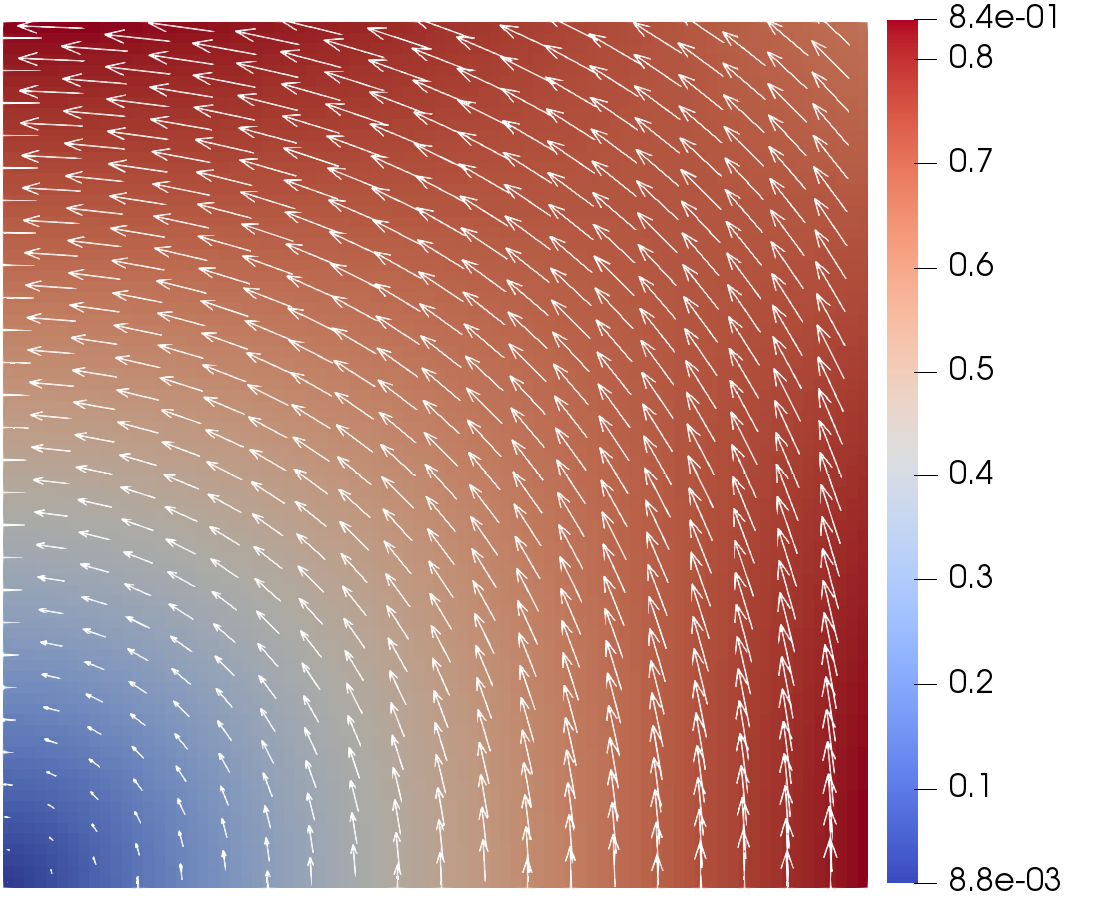
\includegraphics[width=0.5\textwidth]{sincos_exact_v_report.png}}
	\subfloat{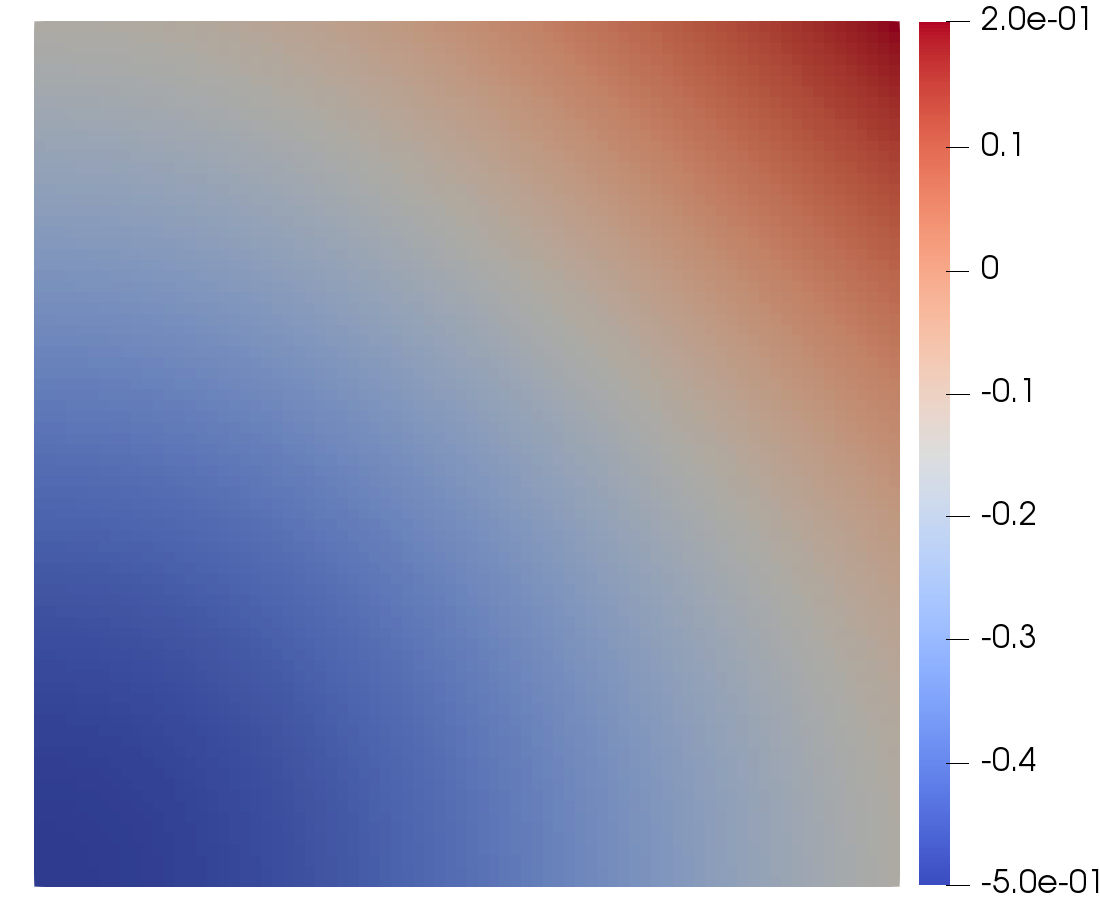
\includegraphics[width=0.5\textwidth]{sincos_exact_p_report.png}}
	\caption[Exact solution of the Sin-Cos test]{Exact solution of the Sin-Cos 
	test \eqref{eq:uexsin}--\eqref{eq:pexsin}. On the left the magnitude of the 
	velocity field, on the right the 
	pressure field.}
	\label{fig:sincosexact}
\end{figure}

The problem is solved over a sequence of five uniform grids, starting from 
$\num{4x4}$ cells and each time halving their size. Both the cases of $\nu=1$ 
and $\nu=\num{e-3}$ are considered, that correspond to $Re=1$ and $Re=\num{e3}$ 
respectively. In Figure~\ref{fig:sin_err} the errors computed are reported 
depending on the square root of the number of cells, while in 
Tables~\ref{tab:sin_lre}--\ref{tab:sin_hre} we can compare directly the 
convergence orders for the different differencing schemes.
\begin{figure}
	\centering
	\subfloat[Upwind, $Re = 1$]{
		% This file was created by matlab2tikz.
%
\definecolor{mycolor1}{rgb}{0.00000,0.44700,0.74100}%
\definecolor{mycolor2}{rgb}{0.85000,0.32500,0.09800}%
\definecolor{mycolor3}{rgb}{0.92900,0.69400,0.12500}%
%
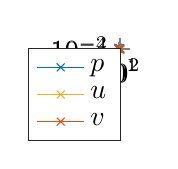
\begin{tikzpicture}

\begin{axis}[%
width=0.951\figwidth,
height=0.75\figwidth,
at={(0\figwidth,0\figwidth)},
scale only axis,
xmode=log,
xmin=4,
xmax=100,
xminorticks=true,
ymode=log,
ymin=1e-05,
ymax=0.1,
yminorticks=true,
axis background/.style={fill=white},
legend style={at={(0.97,0.97)}, anchor=north east, legend cell align=left, align=left, draw=white!15!black}
]
\addplot [color=mycolor1, mark=x, mark options={solid, mycolor1}]
  table[row sep=crcr]{%
4	0.0377253281\\
8	0.016292839\\
16	0.00647505826\\
32	0.00277859939\\
64	0.00131783073\\
};
\addlegendentry{$p$}

\addplot [color=mycolor2, mark=x, mark options={solid, mycolor2}]
  table[row sep=crcr]{%
4	0.00100309389\\
8	0.000409725552\\
16	0.000134946447\\
32	5.06672786e-05\\
64	2.29407924e-05\\
};
\addlegendentry{$u$}

\addplot [color=mycolor3, mark=x, mark options={solid, mycolor3}]
  table[row sep=crcr]{%
4	0.000631316968\\
8	0.000278812074\\
16	0.00010907144\\
32	4.76177485e-05\\
64	2.28652417e-05\\
};
\addlegendentry{$v$}

\addplot [color=white!70!black, forget plot]
  table[row sep=crcr]{%
4	0.00025\\
100	1e-05\\
};
\addplot [color=white!70!black, forget plot]
  table[row sep=crcr]
	\subfloat[Upwind, $Re = \num{e3}$]{
		% This file was created by matlab2tikz.
%
\definecolor{mycolor1}{rgb}{0.00000,0.44700,0.74100}%
\definecolor{mycolor2}{rgb}{0.85000,0.32500,0.09800}%
\definecolor{mycolor3}{rgb}{0.92900,0.69400,0.12500}%
%
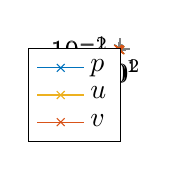
\begin{tikzpicture}

\begin{axis}[%
width=0.951\figwidth,
height=0.75\figwidth,
at={(0\figwidth,0\figwidth)},
scale only axis,
xmode=log,
xmin=4,
xmax=100,
xminorticks=true,
ymode=log,
ymin=0.00266295649,
ymax=0.1,
yminorticks=true,
axis background/.style={fill=white},
legend style={at={(0.97,0.97)}, anchor=north east, legend cell align=left, align=left}
]
\addplot [color=mycolor1, mark=x, mark options={solid, mycolor1}]
  table[row sep=crcr]{%
4	0.0596083589\\
8	0.0364982308\\
16	0.0196434526\\
32	0.00962257784\\
64	0.00434161729\\
};
\addlegendentry{$p$}

\addplot [color=mycolor2, mark=x, mark options={solid, mycolor2}]
  table[row sep=crcr]{%
4	0.0339372138\\
8	0.0206751686\\
16	0.011131246\\
32	0.00559430586\\
64	0.00266295649\\
};
\addlegendentry{$u$}

\addplot [color=mycolor3, mark=x, mark options={solid, mycolor3}]
  table[row sep=crcr]{%
4	0.0347600515\\
8	0.0213374017\\
16	0.0114856296\\
32	0.00577467407\\
64	0.00275450966\\
};
\addlegendentry{$v$}

\addplot [color=white!70!black, forget plot]
  table[row sep=crcr]{%
4	0.06657391225\\
100	0.00266295649\\
};
\addplot [color=white!70!black, forget plot]
  table[row sep=crcr]\\
	\subfloat[Min-Mod, $Re = 1$]{
		% This file was created by matlab2tikz.
%
\definecolor{mycolor1}{rgb}{0.00000,0.44700,0.74100}%
\definecolor{mycolor2}{rgb}{0.85000,0.32500,0.09800}%
\definecolor{mycolor3}{rgb}{0.92900,0.69400,0.12500}%
%
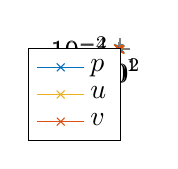
\begin{tikzpicture}

\begin{axis}[%
width=0.951\figwidth,
height=0.75\figwidth,
at={(0\figwidth,0\figwidth)},
scale only axis,
xmode=log,
xmin=4,
xmax=100,
xminorticks=true,
ymode=log,
ymin=1e-05,
ymax=0.1,
yminorticks=true,
axis background/.style={fill=white},
legend style={at={(0.97,0.97)}, anchor=north east, legend cell align=left, align=left}
]
\addplot [color=mycolor1, mark=x, mark options={solid, mycolor1}]
  table[row sep=crcr]{%
4	0.0201961443\\
8	0.00658170291\\
16	0.00181646151\\
32	0.000558641084\\
64	0.000188245776\\
};
\addlegendentry{$p$}

\addplot [color=mycolor2, mark=x, mark options={solid, mycolor2}]
  table[row sep=crcr]{%
4	0.00148598782\\
8	0.00053497283\\
16	0.000150385476\\
32	3.95894587e-05\\
64	1.01636468e-05\\
};
\addlegendentry{$u$}

\addplot [color=mycolor3, mark=x, mark options={solid, mycolor3}]
  table[row sep=crcr]{%
4	0.00119526142\\
8	0.00045470553\\
16	0.000138075359\\
32	3.80865907e-05\\
64	1.00057526e-05\\
};
\addlegendentry{$v$}

\addplot [color=white!70!black, forget plot]
  table[row sep=crcr]{%
4	0.00025\\
100	1e-05\\
};
\addplot [color=white!70!black, forget plot]
  table[row sep=crcr]
	\subfloat[Min-Mod, $Re = \num{e3}$]{
		% This file was created by matlab2tikz.
%
\definecolor{mycolor1}{rgb}{0.00000,0.44700,0.74100}%
\definecolor{mycolor2}{rgb}{0.85000,0.32500,0.09800}%
\definecolor{mycolor3}{rgb}{0.92900,0.69400,0.12500}%
%
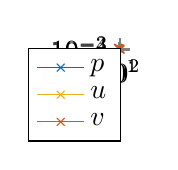
\begin{tikzpicture}

\begin{axis}[%
width=0.951\figwidth,
height=0.75\figwidth,
at={(0\figwidth,0\figwidth)},
scale only axis,
xmode=log,
xmin=4,
xmax=100,
xminorticks=true,
ymode=log,
ymin=0.0001,
ymax=0.0206930353,
yminorticks=true,
axis background/.style={fill=white},
legend style={at={(0.97,0.97)}, anchor=north east, legend cell align=left, align=left}
]
\addplot [color=mycolor1, mark=x, mark options={solid, mycolor1}]
  table[row sep=crcr]{%
4	0.0206930353\\
8	0.0102262223\\
16	0.00364544433\\
32	0.000812298263\\
64	0.000257143964\\
};
\addlegendentry{$p$}

\addplot [color=mycolor2, mark=x, mark options={solid, mycolor2}]
  table[row sep=crcr]{%
4	0.0130268788\\
8	0.00605072242\\
16	0.00243635311\\
32	0.000918041806\\
64	0.000338134479\\
};
\addlegendentry{$u$}

\addplot [color=mycolor3, mark=x, mark options={solid, mycolor3}]
  table[row sep=crcr]{%
4	0.0129926934\\
8	0.00750558766\\
16	0.0037160882\\
32	0.00148526754\\
64	0.000512917943\\
};
\addlegendentry{$v$}

\addplot [color=white!70!black, forget plot]
  table[row sep=crcr]{%
4	0.0025\\
100	0.0001\\
};
\addplot [color=white!70!black, forget plot]
  table[row sep=crcr]\\
	\subfloat[Van Leer, $Re = 1$]{
		% This file was created by matlab2tikz.
%
\definecolor{mycolor1}{rgb}{0.00000,0.44700,0.74100}%
\definecolor{mycolor2}{rgb}{0.85000,0.32500,0.09800}%
\definecolor{mycolor3}{rgb}{0.92900,0.69400,0.12500}%
%
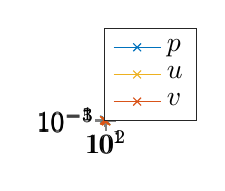
\begin{tikzpicture}

\begin{axis}[%
width=0.951\figwidth,
height=0.75\figwidth,
at={(0\figwidth,0\figwidth)},
scale only axis,
xmode=log,
xmin=4,
xmax=100,
xminorticks=true,
ymode=log,
ymin=8.63199669e-06,
ymax=0.1,
yminorticks=true,
axis background/.style={fill=white},
legend style={at={(0.03,0.03)}, anchor=south west, legend cell align=left, align=left, draw=white!15!black}
]
\addplot [color=mycolor1, mark=x, mark options={solid, mycolor1}]
  table[row sep=crcr]{%
4	0.017335487\\
8	0.0062618753\\
16	0.00193371119\\
32	0.000605597659\\
64	0.000196206927\\
};
\addlegendentry{$p$}

\addplot [color=mycolor2, mark=x, mark options={solid, mycolor2}]
  table[row sep=crcr]{%
4	0.00136409678\\
8	0.000476275877\\
16	0.000131606902\\
32	3.41242821e-05\\
64	8.66824542e-06\\
};
\addlegendentry{$u$}

\addplot [color=mycolor3, mark=x, mark options={solid, mycolor3}]
  table[row sep=crcr]{%
4	0.00114596769\\
8	0.000417513208\\
16	0.000122988533\\
32	3.32359157e-05\\
64	8.63199669e-06\\
};
\addlegendentry{$v$}

\addplot [color=white!70!black, forget plot]
  table[row sep=crcr]{%
4	0.00021579991725\\
100	8.63199669e-06\\
};
\addplot [color=white!70!black, forget plot]
  table[row sep=crcr]
	\subfloat[Van Leer, $Re = \num{e3}$]{
		% This file was created by matlab2tikz.
%
\definecolor{mycolor1}{rgb}{0.00000,0.44700,0.74100}%
\definecolor{mycolor2}{rgb}{0.85000,0.32500,0.09800}%
\definecolor{mycolor3}{rgb}{0.92900,0.69400,0.12500}%
%
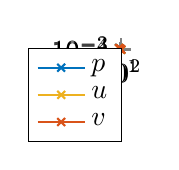
\begin{tikzpicture}

\begin{axis}[%
width=0.951\figwidth,
height=0.75\figwidth,
at={(0\figwidth,0\figwidth)},
scale only axis,
xmode=log,
xmin=4,
xmax=100,
xminorticks=true,
ymode=log,
ymin=0.0001,
ymax=0.01454297,
yminorticks=true,
axis background/.style={fill=white},
legend style={at={(0.97,0.97)}, anchor=north east, legend cell align=left, align=left}
]
\addplot [color=white!70!black, forget plot, line width=0.75pt]
  table[row sep=crcr]{%
4	0.0025\\
100	0.0001\\
};
\addplot [color=white!70!black, forget plot, line width=0.75pt]
  table[row sep=crcr]{%
4	0.0625\\
100	0.0001\\
};
\addplot [color=mycolor1, mark=x, mark options={solid, mycolor1}, line width=0.75pt]
  table[row sep=crcr]{%
4	0.01454297\\
8	0.00653869074\\
16	0.00224775854\\
32	0.0005196908\\
64	0.000249600967\\
};
\addlegendentry{$p$}

\addplot [color=mycolor2, mark=x, mark options={solid, mycolor2}, line width=0.75pt]
  table[row sep=crcr]{%
4	0.0107200353\\
8	0.00466675248\\
16	0.00177426299\\
32	0.000645881865\\
64	0.000238530337\\
};
\addlegendentry{$u$}

\addplot [color=mycolor3, mark=x, mark options={solid, mycolor3}, line width=0.75pt]
  table[row sep=crcr]
	\caption[$L^2$-errors for the Sin-Cos test]{$L^2$-errors for the Sin-Cos 
	test depending on the square root of the number of cells in the grid. 
	The grey lines are the reference lines for the first-order and second-order 
	convergence.}
	\label{fig:sin_err}
\end{figure}

\begin{table}
	\centering
	\[
	\begin{array}{c|ccc}
	\toprule
	& \text{Upwind} & \text{Min-Mod} & \text{Van Leer} \\ 
	\midrule
	p & 1.008 & 1.569 & 1.626\\
	v_x & 1.143 & 1.962 & 1.977\\
	v_y & 1.058 & 1.928 & 1.945\\
	\bottomrule
	\end{array}
	\]
	\caption[Convergence orders with $Re = 1$ for the Sin-Cos 
	test]{Convergence orders with $Re = 1$ for the Sin-Cos test. They are 
	computed considering the last two refinements of the grid.}
	\label{tab:sin_lre}
	\[
	\begin{array}{c|ccc}
	\toprule
	& \text{Upwind} & \text{Min-Mod} & \text{Van Leer} \\ 
	\midrule
	p & 1.148 & 1.659 & 1.058\\
	v_x & 1.071 & 1.441 & 1.437\\
	v_y & 1.068 & 1.533 & 1.560\\
	\bottomrule
	\end{array}
	\]
	\caption[Convergence orders with $Re = \num{e3}$ for the Sin-Cos 
	test]{Convergence orders with $Re = \num{e3}$ for the Sin-Cos test. 
	They are computed considering the last two refinements of the grid.}
	\label{tab:sin_hre}
\end{table}

We observe, as expected, a better behaviour of the TVD methods with respect to 
the upwind method. In Table~\ref{tab:sin_lre} we can see that at $Re=1$ the 
formers show a full second order convergence for the velocity, while for the 
rate is a bit lower; the latter instead shows a first for all the variables. At 
$Re=\num{e3}$ a slight decrease of the rates of the TVD methods occurs also for 
the velocities, but they remain higher then the ones of the upwind method. In 
Table~\ref{tab:sin_hre} we observe a convergence order of 1 for the pressure 
using the Van Leer flux limiter, but looking at Figure~\ref{fig:sin_err} we can 
see that the global trend indicates a convergence of higher order. Moreover it 
can be observed how, thanks to the faster convergence, on the same grid the 
absolute values of the errors reach smaller values using the TVD methods. 
Between the Min-Mod and Van Leer flux limiter it is hard to say which performs 
better, the results are very similar.

Analogous tests with other analytical solutions are reported in the 
Appendix~\ref{app:conv}. They show always a better convergence of the TVD 
methods with respect to the upwind method, but in some cases the convergence 
order of pressure and velocity behave differently.
%
\subsection{Time convergence}
We test the time convergence of the $L^\infty(0,T;L^2(\Omega))$ norm of the 
error of the solution of the Navier-Stokes equations, comparing the results 
obtained with the BE method \eqref{eq:be} and the BDF2 method \eqref{eq:bdf2}.\\
We consider the unsteady version of the 
equations~\eqref{eq:nssteadymass}--\eqref{eq:nssteadymom}:
\begin{align}
	\label{eq:nsunsteadymass} \nabla \cdot \mathbf{v} -h = 0&\\
	\label{eq:nsunsteadymom} \frac{\partial \mathbf{v}}{\partial t} +\nabla 
	\cdot (\mathbf{v} \mathbf{v}^\mathrm{T}) - 
	\nabla \cdot (\nu \nabla \mathbf{v}) + \frac{1}{\varrho}\nabla p  
	-\mathbf{f} = \mathbf{0}&
\end{align}
Again the gravity is neglected and two possible sources $h$ and $\mathbf{f}$ 
are taken into account, moreover all the quantities are considered to be 
non-dimensional.
%
\subsubsection{Unsteady Sin-Cos test}
Let us solve the equations~\eqref{eq:nsunsteadymass}--\eqref{eq:nsunsteadymom} 
over a two dimensional unit domain $\Omega=(0,1)^2$ and in the time interval 
$(0,T)$, with $T=1$. We use the following source terms:
\begin{align}
h &= 0,\\
\mathbf{f} &= 2\Big(\frac{\cos(2t)}{\varrho} + \nu \sin(2t)\Big)[- \cos(x) 
\sin(y), \; 
\cos(y) \sin(x)]^\mathrm{T},
\end{align}
so that, choosing $\varrho=1$, the analytical solution is given by
\begin{align}
\label{eq:uexunssin}	u_\text{ex}(x,y) &= -\cos(x)\sin(y)\sin(2t)\\
v_\text{ex}(x,y) &= \sin(x)\cos(y)\sin(2t)\\
\label{eq:pexunssin}	p_\text{ex}(x,y) &= 
-\frac{\cos(2x)+\sin(2y)}{4}\sin^2(2t),
\end{align}
so it is equal to \eqref{eq:uexsin}--\eqref{eq:pexsin}, used in the steady test 
for the space convergence, except for the modulation over time. We choose 
$\nu=0.1$, so that $Re=10$. Dirichlet boundary conditions for the velocity are 
applied on the whole boundary $\partial \Omega$ using the exact solution. 
Pressure is again fixed  at one point in order to match the exact solution 
\eqref{eq:pexunssin}.

The problem is solved seven times subdividing the time interval $(0,T)$ into 
uniform time-steps and each time time doubling their number, starting from a 
single time-step. Uniform grids of $\num{40x40}$ and $\num{80x80}$ cells are 
employed and as a differencing scheme the TVD method with the Van Leer flux 
limiter \eqref{eq:vl} is used. From Figure~\ref{fig:timeerr} we observe that, 
as expected, the BE method shows a first-order convergence, while the BDF2 
method is of second order. Moreover we notice that, with a grid of 
$\num{40x40}$ cells, in the last refinement the error with the BDF2 method does 
not decrease anymore. This happens because the spatial error becomes 
dominant, indeed refining the grid the convergence order is restored entirely 
for the pressure and almost for the velocity.
\begin{figure}
	\centering
	\subfloat{% This file was created by matlab2tikz.
%
\definecolor{mycolor1}{rgb}{0.00000,0.44700,0.74100}%
\definecolor{mycolor2}{rgb}{0.85000,0.32500,0.09800}%
\definecolor{mycolor3}{rgb}{0.92900,0.69400,0.12500}%
%
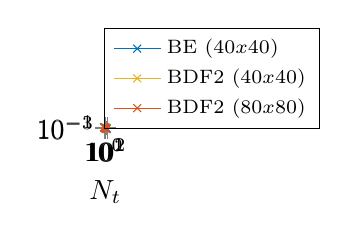
\begin{tikzpicture}

\begin{axis}[%
width=0.99\figwidth,
height=0.8\figwidth,
at={(0\figwidth,0\figwidth)},
scale only axis,
xmode=log,
xmin=1,
xmax=100,
xminorticks=true,
xlabel={$N_t$},
ymode=log,
ymin=0.0001,
ymax=1,
yminorticks=true,
%ylabel style={font=\scriptsize},
%ylabel={$L^\infty$-error},
axis background/.style={fill=white},
legend style={at={(0.03,0.03)}, anchor=south west, legend cell align=left, fill=none,
align=left, font=\scriptsize}
]
\addplot [color=mycolor1, mark=x, mark options={solid, mycolor1}]
  table[row sep=crcr]{%
1	2.91e-1\\
2	1.619e-1\\
4	8.07e-2\\
8	4.17e-2\\
16	2.1e-2\\
32	1.054e-2\\
64	5.31e-3\\
};
\addlegendentry{BE ($\num{40x40}$)}

\addplot [color=mycolor2, mark=x, mark options={solid, mycolor2}]
  table[row sep=crcr]{%
1	2.91e-1\\
2	1e-1\\
4	2.686e-2\\
8	6.81e-3\\
16	1.7e-3\\
32	4.23e-4\\
64	3.816e-4\\
};
\addlegendentry{BDF2 ($\num{40x40}$)}

\addplot [color=mycolor3, mark=x, mark options={solid, mycolor3}]
  table[row sep=crcr]{%
1	2.91e-1\\
2	1e-1\\
4	2.686e-2\\
8	6.814e-3\\
16	1.704e-3\\
32	4.258e-4\\
64	1.347e-4\\
};
\addlegendentry{BDF2 ($\num{80x80}$)}

\addplot [color=white!70!black, forget plot]
  table[row sep=crcr]{%
1	1\\
100	0.01\\
};
\addplot [color=white!70!black, forget plot]
  table[row sep=crcr]
	\subfloat{% This file was created by matlab2tikz.
%
\definecolor{mycolor1}{rgb}{0.00000,0.44700,0.74100}%
\definecolor{mycolor2}{rgb}{0.85000,0.32500,0.09800}%
\definecolor{mycolor3}{rgb}{0.92900,0.69400,0.12500}%
%
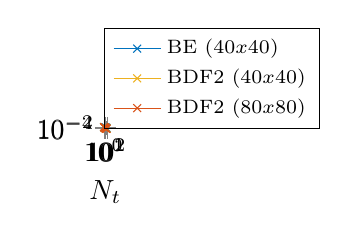
\begin{tikzpicture}

\begin{axis}[%
width=0.99\figwidth,
height=0.8\figwidth,
at={(0\figwidth,0\figwidth)},
scale only axis,
xmode=log,
xmin=1,
xmax=100,
xminorticks=true,
xlabel={$N_t$},
ymode=log,
ymin=1e-5,
ymax=1e-1,
yminorticks=true,
%ylabel style={font=\scriptsize},
%ylabel={$L^\infty$-error},
axis background/.style={fill=white},
legend style={at={(0.03,0.03)}, anchor=south west, legend cell align=left, fill=none,
align=left, font=\scriptsize}
]
\addplot [color=mycolor1, mark=x, mark options={solid, mycolor1}]
  table[row sep=crcr]{%
1	5.516e-2\\
2	3.043e-2\\
4	1.607e-2\\
8	8.216e-3\\
16	4.12e-3\\
32	2.03e-3\\
64	9.712e-4\\
};
\addlegendentry{BE ($\num{40x40}$)}

\addplot [color=mycolor2, mark=x, mark options={solid, mycolor2}]
  table[row sep=crcr]{%
1	5.516e-2\\
2	1.645e-2\\
4	4.8e-3\\
8	1.21e-3\\
16	2.85e-4\\
32	1.3e-4\\
64	1.278e-4\\
};
\addlegendentry{BDF2 ($\num{40x40}$)}

\addplot [color=mycolor3, mark=x, mark options={solid, mycolor3}]
  table[row sep=crcr]{%
1	5.42e-2\\
2	1.647e-2\\
4	4.83e-3\\
8	1.231e-3\\
16	3.024e-4\\
32	7.061e-5\\
64	3.6e-5\\
};
\addlegendentry{BDF2 ($\num{80x80}$)}

\addplot [color=white!70!black, forget plot]
  table[row sep=crcr]{%
1	0.1\\
100	0.001\\
};
\addplot [color=white!70!black, forget plot]
  table[row sep=crcr]
	\caption[$L^\infty(0,T;L^2(\Omega))$-errors for the unsteady Sin-Cos 
	test]{$L^\infty(0,T;L^2(\Omega))$-errors for the unsteady Sin-Cos test 
	depending on the number of time-steps. On the left the errors for the 
	pressure, on the right the error for the magnitude of the velocity. The 
	grey lines are the reference lines for the first-order and second-order 
	convergence.}
	\label{fig:timeerr}
\end{figure}
%
\subsection{Rough channel test} \label{subsec:roughchannel}
We test the behaviour of the TVD methods compared to the upwind method solving 
the unsteady Navier-Stokes equations \eqref{eq:nsmass}--\eqref{eq:nsmom} in 
a two-dimensional channel with a rough (i.e. non-flat) lower boundary. The 
roughness consists of small evenly spaced cavities. Two different 
configurations are studied, one with shallow cavities, depicted in 
Figure~\ref{fig:roughdom}, and another with deeper cavities, depicted in 
Figure~\ref{fig:roughdomdeep}.

On the left boundary $\Gamma_\text{in}$ we set inflow boundary conditions 
\eqref{eq:inflow}, specifying an horizontal velocity
\begin{equation}
	\mathbf{v} = \mathbf{v}_\text{in} = [u_\text{in}, 0]^\mathrm{T}, \quad 
	u_\text{in} = \SI{1}{m/s}.
\end{equation}
On the lower and upper boundaries $\Gamma_w$ we set no-slip boundary conditions 
\eqref{eq:noslip}, while on the right boundary $\Gamma_\text{out}$ we set 
outflow boundary conditions \eqref{eq:outflow}, fixing the value of the pressure
\begin{equation}
	p = p_\text{ext} = \SI{1.1e5}{\pascal}.
\end{equation}
As initial conditions the velocity is set to zero everywhere, while the 
pressure is set to $p_\text{ext}$ everywhere. The density is 
$\varrho=\SI{1}{kg/m^3}$. The gravity contribution in \eqref{eq:nsmom} is 
neglected.
%
\subsubsection{Shallow cavities}
In the case of shallow cavities we use the domain in Figure~\ref{fig:roughdom} 
and we employ a uniform grid of $\num{95x50}$ cells. The problem is then solved 
over the time interval [$0,T$], with $T=\SI{10}{s}$; the initial time-step is 
$\Delta t=\SI{5e-3}{s}$, then it is adapted as explained in 
Section~\ref{sec:algeq}, allowing a maximum time-step of $\SI{0.1}{s}$. 
At first we set $\nu=\SI{5e-4}{m^2/s}$, so that $Re=\num{2e3}$. Since we do not 
have an analytical solution for this problem, we compute a \emph{reference 
solution} using the upwind method over a grid six times finer.

In Figure~\ref{fig:linecompshallow} we compare the profiles of the magnitude 
of the velocity along a section near the end of the channel, at 
$x=\SI{8.75}{m}$, i.e. at the middle of the last cavity.  The TVD solutions 
match the reference one, while the upwind solution shows a small shift, 
especially in the lower part of the channel, above the cavity. So, on a coarse 
grid, we obtain a solution that is the one we would obtain with the upwind 
method on a finer grid. In Table~\ref{tab:errshallow} we can see the $L^2$-norm 
of the errors between the coarse solutions and the reference one, computed 
along the section. As expected, the one related to the upwind method is at 
least one order of magnitude larger than the others. 
\begin{figure}
	\centering
	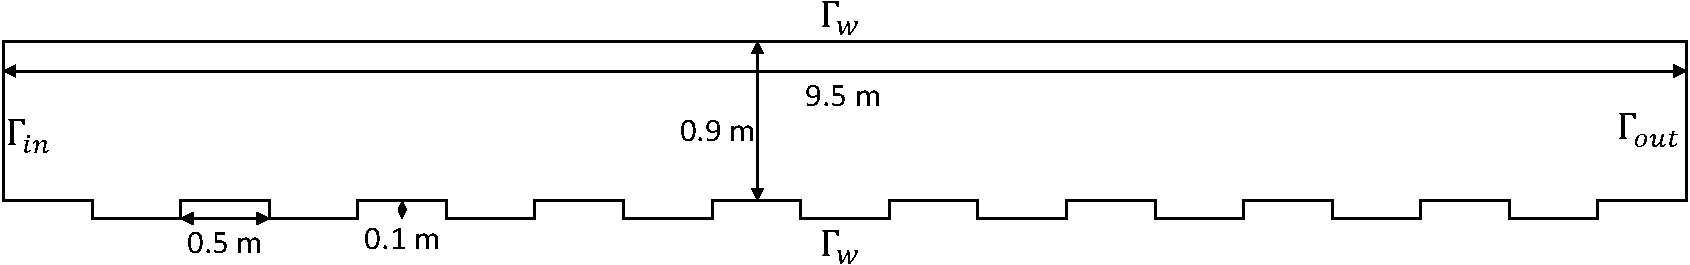
\includegraphics[width=\textwidth]{rough_domain2.pdf}
	\caption[Domain of the rough channel test with shallow cavities]{Domain of 
	the rough channel test with shallow cavities.}
	\label{fig:roughdom}
\end{figure}
\begin{figure}
	\centering
	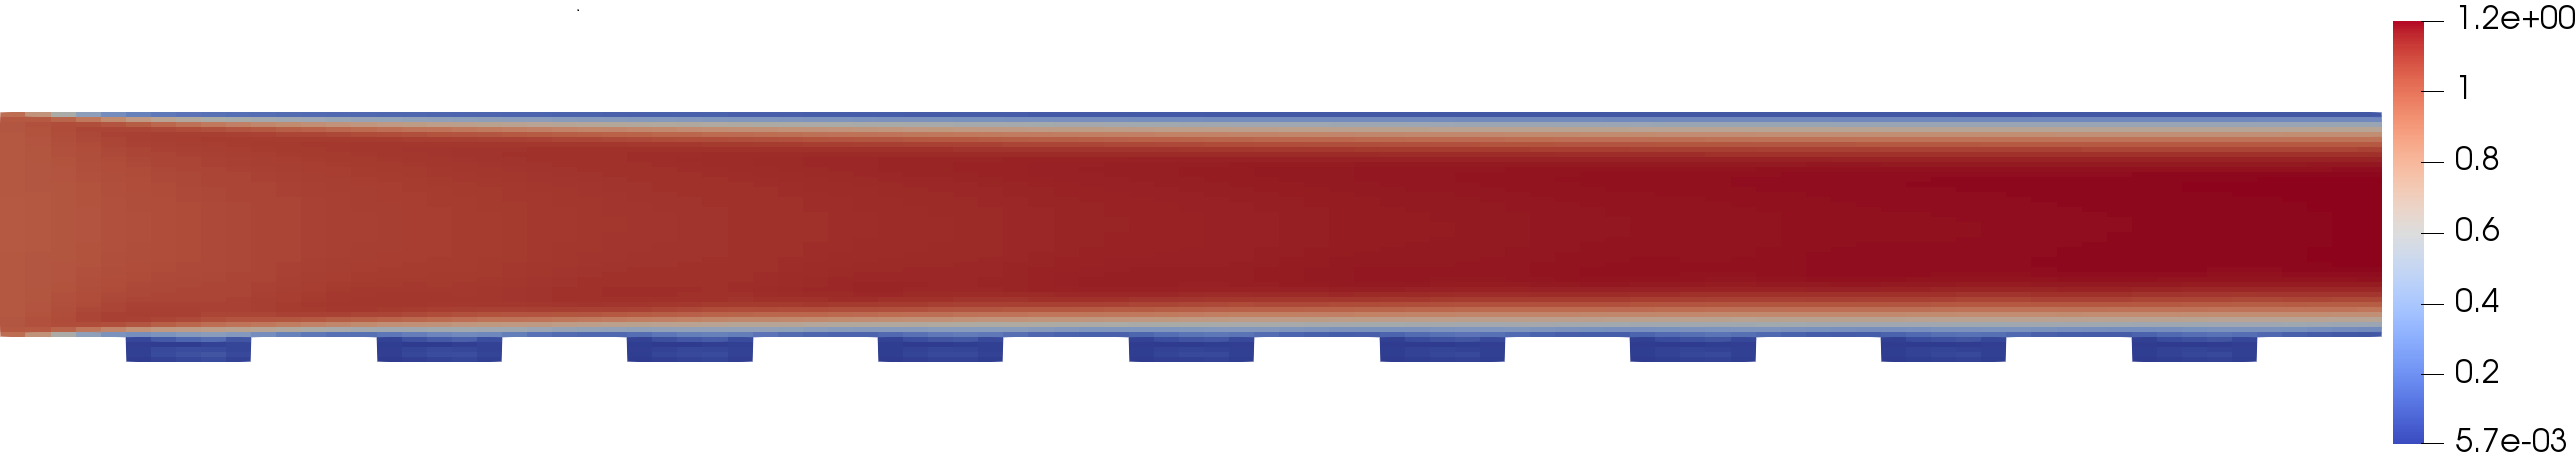
\includegraphics[width=\textwidth]{rough_channel_vl_report.png}
	\caption[Magnitude of the velocity magnitude in the rough channel test with 
	shallow cavities]{Magnitude of the velocity magnitude $[\si{m/s}]$ in the 
	rough channel test with shallow cavities at $t=\SI{10}{s}$. $Re=\num{2e3}$, 
	Van Leer flux limiter.}
	\label{fig:roughchannelvl}
\end{figure}
\begin{figure}
	\centering
	% This file was created by matlab2tikz.
%
\definecolor{mycolor1}{rgb}{0.00000,0.44700,0.74100}%
\definecolor{mycolor2}{rgb}{0.85000,0.32500,0.09800}%
\definecolor{mycolor3}{rgb}{0.92900,0.69400,0.12500}%
\definecolor{mycolor4}{rgb}{0.49400,0.18400,0.55600}%
%
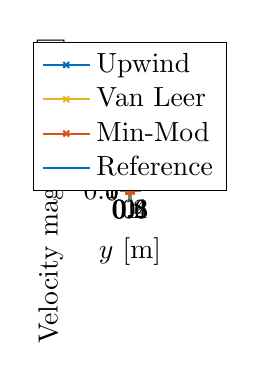
\begin{tikzpicture}

\begin{axis}[%
width=0.951\roughwidth,
height=0.75\roughheight,
at={(0\roughwidth,0\roughheight)},
scale only axis,
xmin=0,
xmax=1,
xlabel={$y$ [m]},
ymin=0,
ymax=1.25,
ylabel={Velocity magnitude [m/s]},
axis background/.style={fill=white},
legend style={at={(0.5,0.03)}, anchor=south, legend cell align=left, align=left}
]
\addplot [color=mycolor1, mark size=1.5pt, mark=x, mark options={solid, mycolor1}, line width=0.75pt]
  table[row sep=crcr]{%
0	0\\
0.01	0.0293662\\
0.03	0.050586\\
0.05	0.0374104\\
0.07	0.00830816\\
0.09	0.0878588\\
0.11	0.203537\\
0.13	0.350154\\
0.15	0.504986\\
0.17	0.648407\\
0.19	0.773425\\
0.21	0.879108\\
0.23	0.965875\\
0.25	1.0347\\
0.27	1.08726\\
0.29	1.12581\\
0.31	1.15286\\
0.33	1.17097\\
0.35	1.18249\\
0.37	1.18938\\
0.39	1.19321\\
0.41	1.19513\\
0.43	1.19595\\
0.45	1.19618\\
0.47	1.19615\\
0.49	1.19606\\
0.51	1.19602\\
0.53	1.19608\\
0.55	1.19627\\
0.57	1.19661\\
0.59	1.19708\\
0.61	1.1977\\
0.63	1.19842\\
0.65	1.19918\\
0.67	1.19986\\
0.69	1.20024\\
0.71	1.19994\\
0.73	1.19831\\
0.75	1.19437\\
0.77	1.18669\\
0.79	1.17327\\
0.81	1.15154\\
0.83	1.11834\\
0.85	1.07018\\
0.87	1.00343\\
0.89	0.914856\\
0.91	0.802051\\
0.93	0.663892\\
0.95	0.500819\\
0.97	0.314904\\
0.99	0.109749\\
1	0\\
};
\addlegendentry{Upwind}

\addplot [color=mycolor2, mark size=1.5pt, mark=x, mark options={solid, mycolor2}, line width=0.75pt]
  table[row sep=crcr]{%
0	0\\
0.01	0.0271697\\
0.03	0.0500789\\
0.05	0.0401093\\
0.07	0.00567534\\
0.09	0.0811925\\
0.11	0.199174\\
0.13	0.35443\\
0.15	0.52202\\
0.17	0.675188\\
0.19	0.804904\\
0.21	0.91139\\
0.23	0.996051\\
0.25	1.06075\\
0.27	1.10807\\
0.29	1.14103\\
0.31	1.16275\\
0.33	1.17616\\
0.35	1.18381\\
0.37	1.1877\\
0.39	1.18933\\
0.41	1.18969\\
0.43	1.18942\\
0.45	1.18894\\
0.47	1.18845\\
0.49	1.18804\\
0.51	1.18779\\
0.53	1.1877\\
0.55	1.18779\\
0.57	1.18804\\
0.59	1.18848\\
0.61	1.18909\\
0.63	1.18985\\
0.65	1.19073\\
0.67	1.19161\\
0.69	1.19229\\
0.71	1.1924\\
0.73	1.19132\\
0.75	1.18802\\
0.77	1.181\\
0.79	1.16815\\
0.81	1.14675\\
0.83	1.11359\\
0.85	1.06512\\
0.87	0.997859\\
0.89	0.908818\\
0.91	0.795828\\
0.93	0.657971\\
0.95	0.495791\\
0.97	0.311428\\
0.99	0.10845\\
1	0\\
};
\addlegendentry{Van Leer}

\addplot [color=mycolor3, mark size=1.5pt, mark=x, mark options={solid, mycolor3}, line width=0.75pt]
  table[row sep=crcr]{%
0	0\\
0.01	0.0272093\\
0.03	0.0494723\\
0.05	0.0389859\\
0.07	0.00595636\\
0.09	0.0812851\\
0.11	0.198804\\
0.13	0.353914\\
0.15	0.5204\\
0.17	0.672249\\
0.19	0.801321\\
0.21	0.907555\\
0.23	0.992249\\
0.25	1.05727\\
0.27	1.10509\\
0.29	1.13867\\
0.31	1.16106\\
0.33	1.17513\\
0.35	1.18335\\
0.37	1.18771\\
0.39	1.18968\\
0.41	1.19029\\
0.43	1.19022\\
0.45	1.18987\\
0.47	1.18946\\
0.49	1.18912\\
0.51	1.18891\\
0.53	1.18887\\
0.55	1.18899\\
0.57	1.18928\\
0.59	1.18974\\
0.61	1.19035\\
0.63	1.19112\\
0.65	1.19197\\
0.67	1.19282\\
0.69	1.19344\\
0.71	1.19347\\
0.73	1.19226\\
0.75	1.18881\\
0.77	1.18163\\
0.79	1.16863\\
0.81	1.14714\\
0.83	1.11395\\
0.85	1.06554\\
0.87	0.998402\\
0.89	0.90948\\
0.91	0.796585\\
0.93	0.658719\\
0.95	0.496437\\
0.97	0.311872\\
0.99	0.108614\\
1	0\\
};
\addlegendentry{Min-Mod}

\addplot [color=mycolor4, line width=0.75pt]
  table[row sep=crcr]{%
0	0\\
0.00166667	0.00492427\\
0.005	0.0138838\\
0.00833333	0.0219483\\
0.0116667	0.0291114\\
0.015	0.0353663\\
0.0183333	0.0407062\\
0.0216667	0.0451241\\
0.025	0.0486134\\
0.0283333	0.051167\\
0.0316667	0.0527786\\
0.035	0.0534416\\
0.0383333	0.0531503\\
0.0416667	0.0518985\\
0.045	0.0496806\\
0.0483333	0.0464911\\
0.0516667	0.042324\\
0.055	0.037174\\
0.0583333	0.0310358\\
0.0616667	0.0239061\\
0.065	0.0157914\\
0.0683333	0.00678684\\
0.0716667	0.00421506\\
0.075	0.0150977\\
0.0783333	0.0273447\\
0.0816667	0.0407005\\
0.085	0.0551595\\
0.0883333	0.0707355\\
0.0916667	0.0874415\\
0.095	0.105279\\
0.0983333	0.124233\\
0.101667	0.144291\\
0.105	0.165438\\
0.108333	0.187646\\
0.111667	0.210875\\
0.115	0.23507\\
0.118333	0.260158\\
0.121667	0.286047\\
0.125	0.312628\\
0.128333	0.33978\\
0.131667	0.367367\\
0.135	0.395245\\
0.138333	0.42327\\
0.141667	0.451298\\
0.145	0.479192\\
0.148333	0.506829\\
0.151667	0.534103\\
0.155	0.560921\\
0.158333	0.587212\\
0.161667	0.612919\\
0.165	0.638002\\
0.168333	0.662436\\
0.171667	0.686204\\
0.175	0.7093\\
0.178333	0.731723\\
0.181667	0.753476\\
0.185	0.774566\\
0.188333	0.795\\
0.191667	0.814784\\
0.195	0.833928\\
0.198333	0.852438\\
0.201667	0.870321\\
0.205	0.887585\\
0.208333	0.904234\\
0.211667	0.920276\\
0.215	0.935716\\
0.218333	0.950561\\
0.221667	0.964818\\
0.225	0.978495\\
0.228333	0.991598\\
0.231667	1.00414\\
0.235	1.01612\\
0.238333	1.02756\\
0.241667	1.03847\\
0.245	1.04885\\
0.248333	1.05871\\
0.251667	1.06808\\
0.255	1.07696\\
0.258333	1.08537\\
0.261667	1.09332\\
0.265	1.10082\\
0.268333	1.10789\\
0.271667	1.11454\\
0.275	1.12079\\
0.278333	1.12664\\
0.281667	1.13213\\
0.285	1.13725\\
0.288333	1.14203\\
0.291667	1.14648\\
0.295	1.15062\\
0.298333	1.15445\\
0.301667	1.158\\
0.305	1.16127\\
0.308333	1.16429\\
0.311667	1.16706\\
0.315	1.1696\\
0.318333	1.17192\\
0.321667	1.17404\\
0.325	1.17597\\
0.328333	1.17771\\
0.331667	1.17929\\
0.335	1.18071\\
0.338333	1.18198\\
0.341667	1.18311\\
0.345	1.18412\\
0.348333	1.18501\\
0.351667	1.18579\\
0.355	1.18647\\
0.358333	1.18706\\
0.361667	1.18757\\
0.365	1.188\\
0.368333	1.18836\\
0.371667	1.18866\\
0.375	1.1889\\
0.378333	1.18908\\
0.381667	1.18923\\
0.385	1.18933\\
0.388333	1.18939\\
0.391667	1.18942\\
0.395	1.18942\\
0.398333	1.1894\\
0.401667	1.18935\\
0.405	1.18928\\
0.408333	1.1892\\
0.411667	1.18911\\
0.415	1.189\\
0.418333	1.18888\\
0.421667	1.18876\\
0.425	1.18863\\
0.428333	1.18849\\
0.431667	1.18836\\
0.435	1.18822\\
0.438333	1.18808\\
0.441667	1.18794\\
0.445	1.1878\\
0.448333	1.18766\\
0.451667	1.18753\\
0.455	1.1874\\
0.458333	1.18727\\
0.461667	1.18715\\
0.465	1.18703\\
0.468333	1.18691\\
0.471667	1.1868\\
0.475	1.1867\\
0.478333	1.1866\\
0.481667	1.18651\\
0.485	1.18642\\
0.488333	1.18634\\
0.491667	1.18626\\
0.495	1.18619\\
0.498333	1.18613\\
0.501667	1.18607\\
0.505	1.18601\\
0.508333	1.18597\\
0.511667	1.18593\\
0.515	1.18589\\
0.518333	1.18586\\
0.521667	1.18584\\
0.525	1.18582\\
0.528333	1.18581\\
0.531667	1.1858\\
0.535	1.1858\\
0.538333	1.18581\\
0.541667	1.18582\\
0.545	1.18584\\
0.548333	1.18586\\
0.551667	1.18589\\
0.555	1.18593\\
0.558333	1.18597\\
0.561667	1.18602\\
0.565	1.18607\\
0.568333	1.18613\\
0.571667	1.18619\\
0.575	1.18626\\
0.578333	1.18634\\
0.581667	1.18642\\
0.585	1.18651\\
0.588333	1.1866\\
0.591667	1.1867\\
0.595	1.18681\\
0.598333	1.18692\\
0.601667	1.18703\\
0.605	1.18716\\
0.608333	1.18729\\
0.611667	1.18742\\
0.615	1.18756\\
0.618333	1.18771\\
0.621667	1.18786\\
0.625	1.18802\\
0.628333	1.18819\\
0.631667	1.18835\\
0.635	1.18853\\
0.638333	1.18871\\
0.641667	1.18889\\
0.645	1.18908\\
0.648333	1.18927\\
0.651667	1.18947\\
0.655	1.18967\\
0.658333	1.18987\\
0.661667	1.19007\\
0.665	1.19028\\
0.668333	1.19048\\
0.671667	1.19068\\
0.675	1.19089\\
0.678333	1.19108\\
0.681667	1.19128\\
0.685	1.19147\\
0.688333	1.19165\\
0.691667	1.19182\\
0.695	1.19197\\
0.698333	1.19212\\
0.701667	1.19224\\
0.705	1.19235\\
0.708333	1.19243\\
0.711667	1.19249\\
0.715	1.19252\\
0.718333	1.19251\\
0.721667	1.19246\\
0.725	1.19237\\
0.728333	1.19223\\
0.731667	1.19204\\
0.735	1.19178\\
0.738333	1.19146\\
0.741667	1.19107\\
0.745	1.19059\\
0.748333	1.19003\\
0.751667	1.18937\\
0.755	1.1886\\
0.758333	1.18772\\
0.761667	1.18671\\
0.765	1.18557\\
0.768333	1.18428\\
0.771667	1.18283\\
0.775	1.18122\\
0.778333	1.17942\\
0.781667	1.17743\\
0.785	1.17523\\
0.788333	1.17282\\
0.791667	1.17016\\
0.795	1.16726\\
0.798333	1.16409\\
0.801667	1.16064\\
0.805	1.15689\\
0.808333	1.15283\\
0.811667	1.14845\\
0.815	1.14372\\
0.818333	1.13862\\
0.821667	1.13315\\
0.825	1.12728\\
0.828333	1.12101\\
0.831667	1.1143\\
0.835	1.10714\\
0.838333	1.09953\\
0.841667	1.09143\\
0.845	1.08284\\
0.848333	1.07374\\
0.851667	1.06411\\
0.855	1.05394\\
0.858333	1.04321\\
0.861667	1.0319\\
0.865	1.02002\\
0.868333	1.00753\\
0.871667	0.994433\\
0.875	0.980713\\
0.878333	0.96636\\
0.881667	0.951363\\
0.885	0.935712\\
0.888333	0.919401\\
0.891667	0.90242\\
0.895	0.884765\\
0.898333	0.866428\\
0.901667	0.847407\\
0.905	0.827698\\
0.908333	0.807298\\
0.911667	0.786206\\
0.915	0.764423\\
0.918333	0.74195\\
0.921667	0.718789\\
0.925	0.694943\\
0.928333	0.670418\\
0.931667	0.645219\\
0.935	0.619353\\
0.938333	0.592828\\
0.941667	0.565653\\
0.945	0.537839\\
0.948333	0.509397\\
0.951667	0.48034\\
0.955	0.45068\\
0.958333	0.420433\\
0.961667	0.389615\\
0.965	0.358241\\
0.968333	0.326328\\
0.971667	0.293895\\
0.975	0.260961\\
0.978333	0.227546\\
0.981667	0.193668\\
0.985	0.15935\\
0.988333	0.124612\\
0.991667	0.0894758\\
0.995	0.0539638\\
0.998333	0.0180982\\
1	0\\
};
\addlegendentry{Reference}
\addplot [color=black, dashed, line width=0.75pt]
  table[row sep=crcr]{%
0.1	0\\
0.1 1.25\\
};
\end{axis}
\end{tikzpicture}%
	\caption[Profile of the magnitude of the velocity in the rough channel with 
	shallow cavities at $Re=\num{2e3}$]{Profile of the magnitude of the 
	velocity $[\si{m/s}]$ in the rough channel with shallow cavities along the 
	section $x=\SI{8.75}{m}$, at $t=\SI{10}{s}$. $Re=\num{2e3}$. The region on 
	the left of the dashed line is inside the cavity.}
	\label{fig:linecompshallow}
\end{figure}
\begin{table}
	\centering
	\[
	\begin{array}{ccc}
	\toprule
	\text{Upwind} & \text{Van Leer} & \text{Van Alabada} \\
	\midrule
	\num{1.708e-4} & \num{9.556e-6} & \num{1.119e-5} \\
	\midrule
	\text{Min-Mod} & \text{Superbee} & \text{MC Limiter} \\
	\midrule
	\num{1.537e-5} &  \SI{8.335e-6} & \num{8.659e-6}\\
	\bottomrule
	\end{array}
	\]
	\caption[$L^2$-errors for the profile of the magnitude of the velocity in 
	the rough channel with shallow cavities at $Re=\num{2e3}$]{$L^2$-errors for 
	the profile of the magnitude of the velocity along a section at 
	$x=\SI{8.75}{m}$ and $t=\SI{10}{s}$ in the rough channel with shallow 
	cavities. $Re = \num{2e3}$.}
	\label{tab:errshallow}
\end{table}

We repeat the test choosing $\nu=\SI{1}{m^2/s}$, so that $Re=1$. In 
Figure~\ref{fig:linecompshallowlre} we see that all the solutions have the same 
profile, moreover in the cavity there is no recirculation. In 
Table~\ref{tab:errshallow_lre} the $L^2$-errors are reported; the upwind one is 
the bigger, but they are all very similar. So, in this situation of low $Re$, 
the benefit of using a high-resolution scheme is reduced.
\begin{figure}
	\centering
	% This file was created by matlab2tikz.
%
\definecolor{mycolor1}{rgb}{0.00000,0.44700,0.74100}%
\definecolor{mycolor2}{rgb}{0.85000,0.32500,0.09800}%
\definecolor{mycolor3}{rgb}{0.92900,0.69400,0.12500}%
\definecolor{mycolor4}{rgb}{0.49400,0.18400,0.55600}%
%
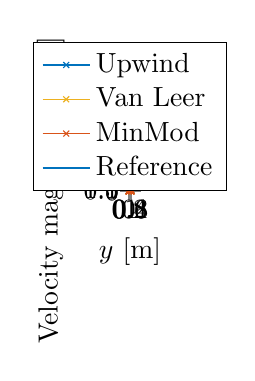
\begin{tikzpicture}

\begin{axis}[%
width=0.951\roughwidth,
height=0.75\roughheight,
at={(0\roughwidth,0\roughheight)},
scale only axis,
xmin=0,
xmax=1,
xlabel={$y$ [m]},
ymin=0,
ymax=1.5,
ylabel={Velocity magnitude [m/s]},
axis background/.style={fill=white},
legend style={at={(0.5,0.03)}, anchor=south, legend cell align=left, align=left}
]
\addplot [color=mycolor1, mark size=1.5pt, mark=x, mark options={solid, mycolor1}]
  table[row sep=crcr]{%
0	0\\
0.01	0.0254229\\
0.03	0.0771412\\
0.05	0.131431\\
0.07	0.189545\\
0.09	0.252263\\
0.11	0.319795\\
0.13	0.391594\\
0.15	0.466634\\
0.17	0.543711\\
0.19	0.621626\\
0.21	0.699267\\
0.23	0.775657\\
0.25	0.849957\\
0.27	0.921463\\
0.29	0.989594\\
0.31	1.05388\\
0.33	1.11392\\
0.35	1.16942\\
0.37	1.22012\\
0.39	1.26583\\
0.41	1.3064\\
0.43	1.34169\\
0.45	1.37161\\
0.47	1.39609\\
0.49	1.41506\\
0.51	1.42849\\
0.53	1.43632\\
0.55	1.43854\\
0.57	1.43512\\
0.59	1.42606\\
0.61	1.41134\\
0.63	1.39096\\
0.65	1.36491\\
0.67	1.3332\\
0.69	1.29582\\
0.71	1.25279\\
0.73	1.2041\\
0.75	1.14977\\
0.77	1.0898\\
0.79	1.02421\\
0.81	0.953007\\
0.83	0.876208\\
0.85	0.79383\\
0.87	0.705892\\
0.89	0.612418\\
0.91	0.513432\\
0.93	0.408963\\
0.95	0.299044\\
0.97	0.183712\\
0.99	0.063011\\
1	0\\
};
\addlegendentry{Upwind}

\addplot [color=mycolor2, mark size=1.5pt, mark=x, mark options={solid, mycolor2}]
  table[row sep=crcr]{%
0	0\\
0.01	0.0256098\\
0.03	0.0776368\\
0.05	0.132183\\
0.07	0.190504\\
0.09	0.253384\\
0.11	0.321031\\
0.13	0.392898\\
0.15	0.467961\\
0.17	0.54502\\
0.19	0.62289\\
0.21	0.700459\\
0.23	0.77675\\
0.25	0.850931\\
0.27	0.922307\\
0.29	0.990298\\
0.31	1.05443\\
0.33	1.11433\\
0.35	1.16969\\
0.37	1.22025\\
0.39	1.26584\\
0.41	1.30628\\
0.43	1.34146\\
0.45	1.37129\\
0.47	1.39566\\
0.49	1.41456\\
0.51	1.42791\\
0.53	1.43568\\
0.55	1.43786\\
0.57	1.4344\\
0.59	1.42531\\
0.61	1.41057\\
0.63	1.39018\\
0.65	1.36413\\
0.67	1.33242\\
0.69	1.29505\\
0.71	1.25203\\
0.73	1.20336\\
0.75	1.14905\\
0.77	1.08912\\
0.79	1.02356\\
0.81	0.952393\\
0.83	0.875636\\
0.85	0.793306\\
0.87	0.70542\\
0.89	0.612002\\
0.91	0.513077\\
0.93	0.408675\\
0.95	0.298828\\
0.97	0.183576\\
0.99	0.0629624\\
1	0\\
};
\addlegendentry{Van Leer}

\addplot [color=mycolor3, mark size=1.5pt, mark=x, mark options={solid, mycolor3}]
  table[row sep=crcr]{%
0	0\\
0.01	0.0255838\\
0.03	0.0775663\\
0.05	0.132074\\
0.07	0.190362\\
0.09	0.253217\\
0.11	0.320848\\
0.13	0.392711\\
0.15	0.467774\\
0.17	0.544841\\
0.19	0.622723\\
0.21	0.70031\\
0.23	0.776621\\
0.25	0.850825\\
0.27	0.92222\\
0.29	0.990231\\
0.31	1.05439\\
0.33	1.1143\\
0.35	1.16968\\
0.37	1.22026\\
0.39	1.26586\\
0.41	1.30632\\
0.43	1.34151\\
0.45	1.37134\\
0.47	1.39573\\
0.49	1.41463\\
0.51	1.42799\\
0.53	1.43577\\
0.55	1.43795\\
0.57	1.4345\\
0.59	1.42541\\
0.61	1.41067\\
0.63	1.39028\\
0.65	1.36422\\
0.67	1.33251\\
0.69	1.29514\\
0.71	1.25212\\
0.73	1.20345\\
0.75	1.14914\\
0.77	1.08919\\
0.79	1.02363\\
0.81	0.952462\\
0.83	0.8757\\
0.85	0.793364\\
0.87	0.705472\\
0.89	0.612048\\
0.91	0.513116\\
0.93	0.408706\\
0.95	0.298851\\
0.97	0.183591\\
0.99	0.0629675\\
1	0\\
};
\addlegendentry{MinMod}

\addplot [color=mycolor4]
  table[row sep=crcr]{%
0	0\\
0.00166667	0.00452198\\
0.005	0.0135298\\
0.00833333	0.0225133\\
0.0116667	0.0314839\\
0.015	0.0404525\\
0.0183333	0.0494296\\
0.0216667	0.0584251\\
0.025	0.0674484\\
0.0283333	0.0765086\\
0.0316667	0.0856141\\
0.035	0.0947727\\
0.0383333	0.103992\\
0.0416667	0.113279\\
0.045	0.122639\\
0.0483333	0.13208\\
0.0516667	0.141606\\
0.055	0.151223\\
0.0583333	0.160933\\
0.0616667	0.170742\\
0.065	0.180653\\
0.0683333	0.190669\\
0.0716667	0.200792\\
0.075	0.211024\\
0.0783333	0.221367\\
0.0816667	0.231823\\
0.085	0.242391\\
0.0883333	0.253073\\
0.0916667	0.263866\\
0.095	0.274774\\
0.0983333	0.285794\\
0.101667	0.296923\\
0.105	0.308161\\
0.108333	0.319508\\
0.111667	0.330959\\
0.115	0.342513\\
0.118333	0.354168\\
0.121667	0.365919\\
0.125	0.377765\\
0.128333	0.3897\\
0.131667	0.401723\\
0.135	0.413829\\
0.138333	0.426013\\
0.141667	0.438273\\
0.145	0.450603\\
0.148333	0.462999\\
0.151667	0.475457\\
0.155	0.487973\\
0.158333	0.50054\\
0.161667	0.513155\\
0.165	0.525812\\
0.168333	0.538508\\
0.171667	0.551237\\
0.175	0.563993\\
0.178333	0.576772\\
0.181667	0.58957\\
0.185	0.602381\\
0.188333	0.615201\\
0.191667	0.628024\\
0.195	0.640846\\
0.198333	0.653662\\
0.201667	0.666468\\
0.205	0.679258\\
0.208333	0.69203\\
0.211667	0.704776\\
0.215	0.717494\\
0.218333	0.730179\\
0.221667	0.742827\\
0.225	0.755434\\
0.228333	0.767995\\
0.231667	0.780507\\
0.235	0.792966\\
0.238333	0.805369\\
0.241667	0.81771\\
0.245	0.829988\\
0.248333	0.842198\\
0.251667	0.854338\\
0.255	0.866403\\
0.258333	0.878391\\
0.261667	0.890298\\
0.265	0.902123\\
0.268333	0.913861\\
0.271667	0.925509\\
0.275	0.937066\\
0.278333	0.948529\\
0.281667	0.959895\\
0.285	0.971162\\
0.288333	0.982327\\
0.291667	0.993388\\
0.295	1.00434\\
0.298333	1.01519\\
0.301667	1.02593\\
0.305	1.03655\\
0.308333	1.04706\\
0.311667	1.05746\\
0.315	1.06773\\
0.318333	1.07789\\
0.321667	1.08792\\
0.325	1.09784\\
0.328333	1.10763\\
0.331667	1.1173\\
0.335	1.12684\\
0.338333	1.13625\\
0.341667	1.14553\\
0.345	1.15468\\
0.348333	1.1637\\
0.351667	1.17258\\
0.355	1.18133\\
0.358333	1.18995\\
0.361667	1.19843\\
0.365	1.20677\\
0.368333	1.21498\\
0.371667	1.22305\\
0.375	1.23097\\
0.378333	1.23876\\
0.381667	1.24641\\
0.385	1.25391\\
0.388333	1.26127\\
0.391667	1.26849\\
0.395	1.27556\\
0.398333	1.28249\\
0.401667	1.28927\\
0.405	1.29591\\
0.408333	1.3024\\
0.411667	1.30875\\
0.415	1.31495\\
0.418333	1.321\\
0.421667	1.3269\\
0.425	1.33266\\
0.428333	1.33826\\
0.431667	1.34372\\
0.435	1.34902\\
0.438333	1.35417\\
0.441667	1.35918\\
0.445	1.36403\\
0.448333	1.36873\\
0.451667	1.37328\\
0.455	1.37768\\
0.458333	1.38191\\
0.461667	1.38601\\
0.465	1.38995\\
0.468333	1.39373\\
0.471667	1.39737\\
0.475	1.40085\\
0.478333	1.40417\\
0.481667	1.40735\\
0.485	1.41036\\
0.488333	1.41323\\
0.491667	1.41594\\
0.495	1.41849\\
0.498333	1.42089\\
0.501667	1.42313\\
0.505	1.42522\\
0.508333	1.42716\\
0.511667	1.42894\\
0.515	1.43056\\
0.518333	1.43202\\
0.521667	1.43334\\
0.525	1.43449\\
0.528333	1.43549\\
0.531667	1.43633\\
0.535	1.43702\\
0.538333	1.43755\\
0.541667	1.43792\\
0.545	1.43814\\
0.548333	1.4382\\
0.551667	1.4381\\
0.555	1.43785\\
0.558333	1.43744\\
0.561667	1.43687\\
0.565	1.43615\\
0.568333	1.43527\\
0.571667	1.43423\\
0.575	1.43304\\
0.578333	1.43168\\
0.581667	1.43017\\
0.585	1.4285\\
0.588333	1.42668\\
0.591667	1.4247\\
0.595	1.42256\\
0.598333	1.42026\\
0.601667	1.41781\\
0.605	1.4152\\
0.608333	1.41243\\
0.611667	1.40951\\
0.615	1.40642\\
0.618333	1.40319\\
0.621667	1.39979\\
0.625	1.39623\\
0.628333	1.39252\\
0.631667	1.38865\\
0.635	1.38462\\
0.638333	1.38044\\
0.641667	1.3761\\
0.645	1.3716\\
0.648333	1.36694\\
0.651667	1.36213\\
0.655	1.35715\\
0.658333	1.35202\\
0.661667	1.34674\\
0.665	1.34129\\
0.668333	1.33569\\
0.671667	1.32993\\
0.675	1.32402\\
0.678333	1.31794\\
0.681667	1.31171\\
0.685	1.30532\\
0.688333	1.29878\\
0.691667	1.29207\\
0.695	1.28521\\
0.698333	1.2782\\
0.701667	1.27102\\
0.705	1.26369\\
0.708333	1.2562\\
0.711667	1.24855\\
0.715	1.24075\\
0.718333	1.23279\\
0.721667	1.22467\\
0.725	1.2164\\
0.728333	1.20797\\
0.731667	1.19938\\
0.735	1.19064\\
0.738333	1.18174\\
0.741667	1.17268\\
0.745	1.16346\\
0.748333	1.15409\\
0.751667	1.14456\\
0.755	1.13488\\
0.758333	1.12504\\
0.761667	1.11504\\
0.765	1.10489\\
0.768333	1.09458\\
0.771667	1.08411\\
0.775	1.07349\\
0.778333	1.06271\\
0.781667	1.05177\\
0.785	1.04068\\
0.788333	1.02943\\
0.791667	1.01803\\
0.795	1.00647\\
0.798333	0.994758\\
0.801667	0.982888\\
0.805	0.970862\\
0.808333	0.958681\\
0.811667	0.946344\\
0.815	0.933851\\
0.818333	0.921203\\
0.821667	0.9084\\
0.825	0.895442\\
0.828333	0.882328\\
0.831667	0.86906\\
0.835	0.855636\\
0.838333	0.842058\\
0.841667	0.828325\\
0.845	0.814438\\
0.848333	0.800395\\
0.851667	0.786198\\
0.855	0.771847\\
0.858333	0.757342\\
0.861667	0.742682\\
0.865	0.727868\\
0.868333	0.712901\\
0.871667	0.697779\\
0.875	0.682504\\
0.878333	0.667075\\
0.881667	0.651492\\
0.885	0.635756\\
0.888333	0.619867\\
0.891667	0.603825\\
0.895	0.587629\\
0.898333	0.571281\\
0.901667	0.55478\\
0.905	0.538126\\
0.908333	0.521319\\
0.911667	0.504361\\
0.915	0.48725\\
0.918333	0.469987\\
0.921667	0.452572\\
0.925	0.435005\\
0.928333	0.417287\\
0.931667	0.399417\\
0.935	0.381396\\
0.938333	0.363224\\
0.941667	0.344901\\
0.945	0.326427\\
0.948333	0.307803\\
0.951667	0.289028\\
0.955	0.270103\\
0.958333	0.251028\\
0.961667	0.231803\\
0.965	0.212428\\
0.968333	0.192904\\
0.971667	0.173231\\
0.975	0.153409\\
0.978333	0.133438\\
0.981667	0.113319\\
0.985	0.0930514\\
0.988333	0.0726357\\
0.991667	0.0520722\\
0.995	0.0313611\\
0.998333	0.0105027\\
1	0\\
};
\addlegendentry{Reference}
\addplot [color=black, dashed]
  table[row sep=crcr]{%
0.1	0\\
0.1 1.5\\
};
\end{axis}
\end{tikzpicture}%
	\caption[Profile of the magnitude of the velocity in the rough channel with 
	shallow cavities at $Re=1$]{Profile of the magnitude of the velocity 
	$[\si{m/s}]$ in the rough channel with shallow cavities along the section 
	$x=\SI{8.75}{m}$, at $t=\SI{5}{s}$. $Re=1$. The region on the left of the 
	dashed line is inside the cavity.}
	\label{fig:linecompshallowlre}
\end{figure}
\begin{table}
	\centering
	\[
	\begin{array}{ccc}
	\toprule
	\text{Upwind} & \text{Van Leer} & \text{Van Alabada}\\
	\midrule
	\num{3.431e-6} & \num{2.917e-6} & \num{2.937e-6}\\
	\midrule
	\text{Min-Mod} & \text{Superbee} & \text{MC Limiter} \\ 
	\midrule
	\num{2.956e-6} & \num{2.899e-6} & \num{2.902e-6}\\
	\bottomrule
	\end{array}
	\]
	\caption[$L^2$-errors for the profile of the magnitude of the velocity in 
	the rough channel with shallow cavities at $Re=1$]{$L^2$-errors for the 
	profile of the magnitude of the velocity along a section at 
	$x=\SI{8.75}{m}$ and $t=\SI{5}{s}$ in the rough channel with shallow 
	cavities. $Re = 1$.}
	\label{tab:errshallow_lre}
\end{table}
%
\subsubsection{Deep cavities}
In the case of deep cavities we use the domain in Figure~\ref{fig:roughdomdeep} 
and we employ a uniform grid of $\num{95x70}$ cells. Again we solve until 
$T=\SI{10}{s}$, starting from an initial time-step of $\SI{e-3}{s}$. We set 
$\nu=\SI{5e-4}{m^2/s}$, so that $Re=\num{2.8e3}$. As before we compute a 
reference solution over a grid six times finer.

In Figure~\ref{fig:linecompdeep} we compare the profiles of the magnitude of 
the velocity along the section at $x=\SI{8.75}{m}$. Now the biggest differences 
are in the region inside the cavity, where the recirculation occurs. The upwind 
method, with its numerical diffusion, smooths the profile, while the TVD 
methods produce a more accurate result, even if they do not match exactly the 
reference solution. Indeed, looking at the $L^2$-errors reported in 
Table~\ref{tab:errdeep}, we see that the upwind has again the largest error, 
but the difference with the other schemes is reduced with respect to the 
previous case of shallow cavities.
\begin{figure}
	\centering
	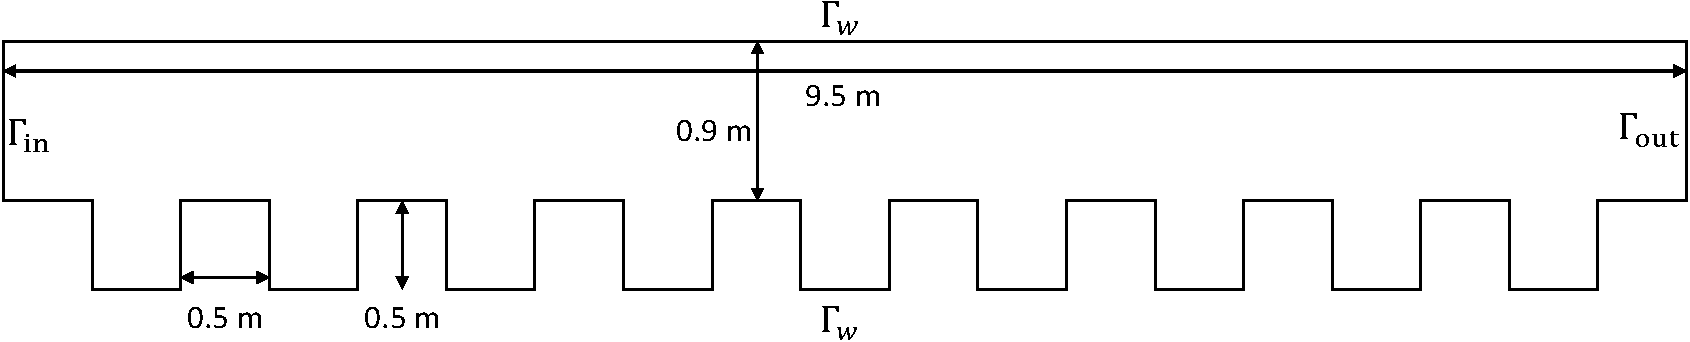
\includegraphics[width=\textwidth]{rough_domain_highstep2.pdf}
	\caption[Domain of the rough channel test with deep cavities]{Domain of the 
	rough channel test with deep cavities.}
	\label{fig:roughdomdeep}
\end{figure}
\begin{figure}
	\centering
	% This file was created by matlab2tikz.
%
\definecolor{mycolor1}{rgb}{0.00000,0.44700,0.74100}%
\definecolor{mycolor2}{rgb}{0.85000,0.32500,0.09800}%
\definecolor{mycolor3}{rgb}{0.92900,0.69400,0.12500}%
\definecolor{mycolor4}{rgb}{0.49400,0.18400,0.55600}%
%
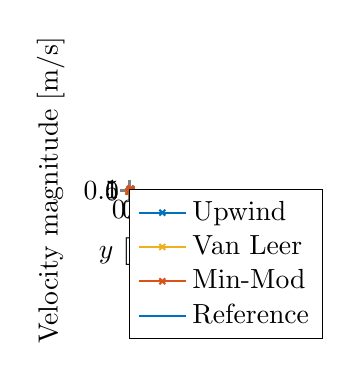
\begin{tikzpicture}

\begin{axis}[%
width=0.951\roughwidth,
height=0.75\roughheight,
at={(0\roughwidth,0\roughheight)},
scale only axis,
xmin=0,
xmax=1.4,
xlabel={$y$ [m]},
ymin=0,
ymax=1.25,
ylabel={Velocity magnitude [m/s]},
axis background/.style={fill=white},
legend style={at={(0.03,0.97)}, anchor=north west, legend cell align=left, align=left}
]

\addplot [color=mycolor1, mark size=1.5pt, mark=x, mark options={solid, mycolor1}, line width=0.75pt]
  table[row sep=crcr]{%
0	0\\
0.01	0.00885222\\
0.03	0.0227802\\
0.05	0.0327807\\
0.07	0.0393192\\
0.09	0.043122\\
0.11	0.0448784\\
0.13	0.0451341\\
0.15	0.0442874\\
0.17	0.0426208\\
0.19	0.0403378\\
0.21	0.037597\\
0.23	0.0345472\\
0.25	0.0313691\\
0.27	0.0283253\\
0.29	0.0258075\\
0.31	0.0243184\\
0.33	0.024277\\
0.35	0.0257093\\
0.37	0.0283224\\
0.39	0.0319839\\
0.41	0.0370173\\
0.43	0.044611\\
0.45	0.0576046\\
0.47	0.0818451\\
0.49	0.128213\\
0.51	0.214615\\
0.53	0.35431\\
0.55	0.509962\\
0.57	0.654372\\
0.59	0.77967\\
0.61	0.885193\\
0.63	0.971543\\
0.65	1.03985\\
0.67	1.0919\\
0.69	1.12994\\
0.71	1.15654\\
0.73	1.17426\\
0.75	1.18543\\
0.77	1.19201\\
0.79	1.19557\\
0.81	1.19723\\
0.83	1.1978\\
0.85	1.19779\\
0.87	1.19754\\
0.89	1.19723\\
0.91	1.19698\\
0.93	1.19685\\
0.95	1.19686\\
0.97	1.19703\\
0.99	1.19736\\
1.01	1.19783\\
1.03	1.19841\\
1.05	1.19906\\
1.07	1.19964\\
1.09	1.19992\\
1.11	1.19953\\
1.13	1.19783\\
1.15	1.19384\\
1.17	1.1861\\
1.19	1.17264\\
1.21	1.15086\\
1.23	1.11762\\
1.25	1.06938\\
1.27	1.00254\\
1.29	0.913831\\
1.31	0.800848\\
1.33	0.662508\\
1.35	0.499366\\
1.37	0.313659\\
1.39	0.109156\\
1.4	0\\
};
\addlegendentry{Upwind}

\addplot [color=mycolor2, mark size=1.5pt, mark=x, mark options={solid, mycolor2}, line width=0.75pt]
  table[row sep=crcr]{%
0	0\\
0.01	0.0122335\\
0.03	0.0324848\\
0.05	0.0480886\\
0.07	0.0588624\\
0.09	0.0654371\\
0.11	0.0686113\\
0.13	0.0688211\\
0.15	0.0669287\\
0.17	0.0627025\\
0.19	0.0563737\\
0.21	0.0484432\\
0.23	0.0398216\\
0.25	0.0319033\\
0.27	0.0265586\\
0.29	0.0256695\\
0.31	0.0288832\\
0.33	0.0340499\\
0.35	0.0396606\\
0.37	0.0450472\\
0.39	0.0499693\\
0.41	0.0545328\\
0.43	0.0595794\\
0.45	0.0677895\\
0.47	0.0859627\\
0.49	0.128135\\
0.51	0.214164\\
0.53	0.35562\\
0.55	0.519342\\
0.57	0.670222\\
0.59	0.798895\\
0.61	0.905422\\
0.63	0.991025\\
0.65	1.05726\\
0.67	1.10635\\
0.69	1.14101\\
0.71	1.16412\\
0.73	1.17855\\
0.75	1.18688\\
0.77	1.19113\\
0.79	1.19289\\
0.81	1.19325\\
0.83	1.1929\\
0.85	1.19227\\
0.87	1.19163\\
0.89	1.19106\\
0.91	1.19067\\
0.93	1.19044\\
0.95	1.19037\\
0.97	1.1905\\
0.99	1.19084\\
1.01	1.19135\\
1.03	1.19204\\
1.05	1.19284\\
1.07	1.19365\\
1.09	1.19427\\
1.11	1.19434\\
1.13	1.19322\\
1.15	1.1899\\
1.17	1.18285\\
1.19	1.16996\\
1.21	1.14851\\
1.23	1.11525\\
1.25	1.06662\\
1.27	0.999152\\
1.29	0.909811\\
1.31	0.796478\\
1.33	0.658286\\
1.35	0.495815\\
1.37	0.311267\\
1.39	0.108298\\
1.4	0\\
};
\addlegendentry{Van Leer}

\addplot [color=mycolor3, mark size=1.5pt, mark=x, mark options={solid, mycolor3}, line width=0.75pt]
  table[row sep=crcr]{%
0	0\\
0.01	0.0113419\\
0.03	0.0297822\\
0.05	0.0438459\\
0.07	0.0535293\\
0.09	0.0594514\\
0.11	0.0623285\\
0.13	0.0627341\\
0.15	0.0613312\\
0.17	0.0581295\\
0.19	0.0533229\\
0.21	0.0472654\\
0.23	0.040544\\
0.25	0.0340756\\
0.27	0.0291588\\
0.29	0.0272168\\
0.31	0.0284915\\
0.33	0.0317763\\
0.35	0.0359173\\
0.37	0.0402998\\
0.39	0.0446982\\
0.41	0.0493064\\
0.43	0.0551453\\
0.45	0.0648297\\
0.47	0.0848545\\
0.49	0.128268\\
0.51	0.214524\\
0.53	0.355773\\
0.55	0.518594\\
0.57	0.668691\\
0.59	0.796856\\
0.61	0.903066\\
0.63	0.988544\\
0.65	1.05485\\
0.67	1.10418\\
0.69	1.13918\\
0.71	1.16273\\
0.73	1.17764\\
0.75	1.1864\\
0.77	1.19104\\
0.79	1.19311\\
0.81	1.19369\\
0.83	1.19352\\
0.85	1.19301\\
0.87	1.19243\\
0.89	1.19193\\
0.91	1.19158\\
0.93	1.19138\\
0.95	1.19133\\
0.97	1.19148\\
0.99	1.19181\\
1.01	1.19232\\
1.03	1.19298\\
1.05	1.19375\\
1.07	1.19452\\
1.09	1.19508\\
1.11	1.19505\\
1.13	1.19379\\
1.15	1.1903\\
1.17	1.18309\\
1.19	1.17005\\
1.21	1.14852\\
1.23	1.11526\\
1.25	1.06673\\
1.27	0.999415\\
1.29	0.910241\\
1.31	0.797042\\
1.33	0.658892\\
1.35	0.496348\\
1.37	0.311635\\
1.39	0.108434\\
1.4	0\\
};
\addlegendentry{Min-Mod}

\addplot [color=mycolor4, line width=0.75pt]
  table[row sep=crcr]{%
0	0\\
0.00166667	0.00162965\\
0.005	0.00480799\\
0.00833333	0.00790634\\
0.0116667	0.0109252\\
0.015	0.013865\\
0.0183333	0.0167258\\
0.0216667	0.019508\\
0.025	0.022212\\
0.0283333	0.0248383\\
0.0316667	0.0273878\\
0.035	0.0298613\\
0.0383333	0.03226\\
0.0416667	0.0345853\\
0.045	0.0368385\\
0.0483333	0.0390211\\
0.0516667	0.0411348\\
0.055	0.0431809\\
0.0583333	0.045161\\
0.0616667	0.0470764\\
0.065	0.0489283\\
0.0683333	0.0507176\\
0.0716667	0.0524452\\
0.075	0.0541115\\
0.0783333	0.055717\\
0.0816667	0.0572619\\
0.085	0.0587457\\
0.0883333	0.0601683\\
0.0916667	0.0615291\\
0.095	0.0628271\\
0.0983333	0.0640617\\
0.101667	0.0652316\\
0.105	0.0663357\\
0.108333	0.0673728\\
0.111667	0.0683414\\
0.115	0.0692403\\
0.118333	0.070068\\
0.121667	0.0708231\\
0.125	0.0715044\\
0.128333	0.0721104\\
0.131667	0.0726401\\
0.135	0.0730923\\
0.138333	0.0734658\\
0.141667	0.0737601\\
0.145	0.0739741\\
0.148333	0.0741073\\
0.151667	0.0741594\\
0.155	0.0741298\\
0.158333	0.0740188\\
0.161667	0.0738262\\
0.165	0.0735523\\
0.168333	0.0731975\\
0.171667	0.0727624\\
0.175	0.0722478\\
0.178333	0.0716544\\
0.181667	0.0709837\\
0.185	0.0702367\\
0.188333	0.0694149\\
0.191667	0.0685199\\
0.195	0.0675533\\
0.198333	0.0665172\\
0.201667	0.0654135\\
0.205	0.0642444\\
0.208333	0.0630124\\
0.211667	0.0617197\\
0.215	0.0603692\\
0.218333	0.0589636\\
0.221667	0.0575058\\
0.225	0.055999\\
0.228333	0.0544466\\
0.231667	0.0528522\\
0.235	0.0512197\\
0.238333	0.0495534\\
0.241667	0.0478579\\
0.245	0.0461384\\
0.248333	0.0444006\\
0.251667	0.042651\\
0.255	0.0408971\\
0.258333	0.0391474\\
0.261667	0.0374118\\
0.265	0.0357016\\
0.268333	0.0340304\\
0.271667	0.032414\\
0.275	0.0308707\\
0.278333	0.0294217\\
0.281667	0.0280915\\
0.285	0.026907\\
0.288333	0.025897\\
0.291667	0.0250911\\
0.295	0.0245166\\
0.298333	0.0241958\\
0.301667	0.0241434\\
0.305	0.024363\\
0.308333	0.0248475\\
0.311667	0.0255795\\
0.315	0.0265348\\
0.318333	0.0276856\\
0.321667	0.0290029\\
0.325	0.0304586\\
0.328333	0.0320267\\
0.331667	0.0336841\\
0.335	0.0354105\\
0.338333	0.0371883\\
0.341667	0.0390024\\
0.345	0.0408399\\
0.348333	0.0426898\\
0.351667	0.0445425\\
0.355	0.04639\\
0.358333	0.048225\\
0.361667	0.0500416\\
0.365	0.0518343\\
0.368333	0.0535986\\
0.371667	0.0553303\\
0.375	0.0570259\\
0.378333	0.0586824\\
0.381667	0.060297\\
0.385	0.0618676\\
0.388333	0.0633923\\
0.391667	0.0648697\\
0.395	0.0662986\\
0.398333	0.0676785\\
0.401667	0.0690093\\
0.405	0.0702916\\
0.408333	0.0715265\\
0.411667	0.072716\\
0.415	0.0738628\\
0.418333	0.0749713\\
0.421667	0.076047\\
0.425	0.0770969\\
0.428333	0.0781306\\
0.431667	0.0791597\\
0.435	0.0801992\\
0.438333	0.0812674\\
0.441667	0.0823869\\
0.445	0.0835853\\
0.448333	0.084896\\
0.451667	0.0863585\\
0.455	0.08802\\
0.458333	0.0899355\\
0.461667	0.0921692\\
0.465	0.0947941\\
0.468333	0.0978929\\
0.471667	0.101558\\
0.475	0.105891\\
0.478333	0.111\\
0.481667	0.117001\\
0.485	0.124015\\
0.488333	0.13216\\
0.491667	0.141554\\
0.495	0.152307\\
0.498333	0.164518\\
0.501667	0.178267\\
0.505	0.193612\\
0.508333	0.210581\\
0.511667	0.229172\\
0.515	0.249346\\
0.518333	0.271026\\
0.521667	0.294097\\
0.525	0.318416\\
0.528333	0.3438\\
0.531667	0.370031\\
0.535	0.396864\\
0.538333	0.42408\\
0.541667	0.451482\\
0.545	0.478885\\
0.548333	0.506133\\
0.551667	0.533085\\
0.555	0.559629\\
0.558333	0.585678\\
0.561667	0.611162\\
0.565	0.636036\\
0.568333	0.660269\\
0.571667	0.683845\\
0.575	0.706758\\
0.578333	0.729008\\
0.581667	0.750601\\
0.585	0.771545\\
0.588333	0.79185\\
0.591667	0.811525\\
0.595	0.83058\\
0.598333	0.849024\\
0.601667	0.866863\\
0.605	0.884107\\
0.608333	0.900759\\
0.611667	0.916826\\
0.615	0.932313\\
0.618333	0.947225\\
0.621667	0.961569\\
0.625	0.975348\\
0.628333	0.988573\\
0.631667	1.00125\\
0.635	1.01338\\
0.638333	1.02498\\
0.641667	1.03605\\
0.645	1.04661\\
0.648333	1.05667\\
0.651667	1.06623\\
0.655	1.07531\\
0.658333	1.08392\\
0.661667	1.09207\\
0.665	1.09978\\
0.668333	1.10705\\
0.671667	1.11391\\
0.675	1.12035\\
0.678333	1.12641\\
0.681667	1.13209\\
0.685	1.1374\\
0.688333	1.14237\\
0.691667	1.147\\
0.695	1.15131\\
0.698333	1.15531\\
0.701667	1.15901\\
0.705	1.16244\\
0.708333	1.1656\\
0.711667	1.16851\\
0.715	1.17118\\
0.718333	1.17363\\
0.721667	1.17586\\
0.725	1.17789\\
0.728333	1.17974\\
0.731667	1.18141\\
0.735	1.18291\\
0.738333	1.18425\\
0.741667	1.18546\\
0.745	1.18653\\
0.748333	1.18747\\
0.751667	1.18831\\
0.755	1.18903\\
0.758333	1.18966\\
0.761667	1.1902\\
0.765	1.19066\\
0.768333	1.19104\\
0.771667	1.19135\\
0.775	1.19161\\
0.778333	1.19181\\
0.781667	1.19195\\
0.785	1.19206\\
0.788333	1.19212\\
0.791667	1.19214\\
0.795	1.19214\\
0.798333	1.19211\\
0.801667	1.19205\\
0.805	1.19197\\
0.808333	1.19188\\
0.811667	1.19177\\
0.815	1.19164\\
0.818333	1.19151\\
0.821667	1.19136\\
0.825	1.19121\\
0.828333	1.19106\\
0.831667	1.1909\\
0.835	1.19073\\
0.838333	1.19057\\
0.841667	1.19041\\
0.845	1.19025\\
0.848333	1.19009\\
0.851667	1.18993\\
0.855	1.18977\\
0.858333	1.18962\\
0.861667	1.18947\\
0.865	1.18933\\
0.868333	1.18919\\
0.871667	1.18906\\
0.875	1.18893\\
0.878333	1.18881\\
0.881667	1.18869\\
0.885	1.18858\\
0.888333	1.18847\\
0.891667	1.18838\\
0.895	1.18828\\
0.898333	1.1882\\
0.901667	1.18812\\
0.905	1.18804\\
0.908333	1.18797\\
0.911667	1.18791\\
0.915	1.18786\\
0.918333	1.18781\\
0.921667	1.18776\\
0.925	1.18773\\
0.928333	1.1877\\
0.931667	1.18767\\
0.935	1.18765\\
0.938333	1.18764\\
0.941667	1.18763\\
0.945	1.18763\\
0.948333	1.18764\\
0.951667	1.18765\\
0.955	1.18767\\
0.958333	1.18769\\
0.961667	1.18772\\
0.965	1.18776\\
0.968333	1.1878\\
0.971667	1.18785\\
0.975	1.1879\\
0.978333	1.18797\\
0.981667	1.18803\\
0.985	1.18811\\
0.988333	1.18818\\
0.991667	1.18827\\
0.995	1.18836\\
0.998333	1.18846\\
1.00167	1.18856\\
1.005	1.18867\\
1.00833	1.18879\\
1.01167	1.18891\\
1.015	1.18904\\
1.01833	1.18917\\
1.02167	1.18931\\
1.025	1.18946\\
1.02833	1.18961\\
1.03167	1.18977\\
1.035	1.18993\\
1.03833	1.1901\\
1.04167	1.19027\\
1.045	1.19045\\
1.04833	1.19063\\
1.05167	1.19081\\
1.055	1.191\\
1.05833	1.19119\\
1.06167	1.19139\\
1.065	1.19158\\
1.06833	1.19177\\
1.07167	1.19197\\
1.075	1.19216\\
1.07833	1.19235\\
1.08167	1.19253\\
1.085	1.19271\\
1.08833	1.19288\\
1.09167	1.19305\\
1.095	1.1932\\
1.09833	1.19333\\
1.10167	1.19345\\
1.105	1.19355\\
1.10833	1.19362\\
1.11167	1.19367\\
1.115	1.19369\\
1.11833	1.19368\\
1.12167	1.19363\\
1.125	1.19353\\
1.12833	1.19338\\
1.13167	1.19319\\
1.135	1.19293\\
1.13833	1.1926\\
1.14167	1.1922\\
1.145	1.19172\\
1.14833	1.19115\\
1.15167	1.19049\\
1.155	1.18971\\
1.15833	1.18883\\
1.16167	1.18782\\
1.165	1.18667\\
1.16833	1.18538\\
1.17167	1.18393\\
1.175	1.18231\\
1.17833	1.18051\\
1.18167	1.17852\\
1.185	1.17632\\
1.18833	1.17389\\
1.19167	1.17123\\
1.195	1.16832\\
1.19833	1.16515\\
1.20167	1.1617\\
1.205	1.15794\\
1.20833	1.15388\\
1.21167	1.14949\\
1.215	1.14475\\
1.21833	1.13965\\
1.22167	1.13417\\
1.225	1.12829\\
1.22833	1.12201\\
1.23167	1.11529\\
1.235	1.10812\\
1.23833	1.1005\\
1.24167	1.09239\\
1.245	1.08378\\
1.24833	1.07466\\
1.25167	1.06502\\
1.255	1.05483\\
1.25833	1.04408\\
1.26167	1.03276\\
1.265	1.02085\\
1.26833	1.00835\\
1.27167	0.995228\\
1.275	0.981485\\
1.27833	0.967108\\
1.28167	0.952085\\
1.285	0.936409\\
1.28833	0.92007\\
1.29167	0.903062\\
1.295	0.885377\\
1.29833	0.867011\\
1.30167	0.847959\\
1.305	0.828218\\
1.30833	0.807786\\
1.31167	0.786662\\
1.315	0.764846\\
1.31833	0.742339\\
1.32167	0.719144\\
1.325	0.695264\\
1.32833	0.670704\\
1.33167	0.645471\\
1.335	0.619571\\
1.33833	0.593012\\
1.34167	0.565805\\
1.345	0.537959\\
1.34833	0.509487\\
1.35167	0.480401\\
1.355	0.450714\\
1.35833	0.420443\\
1.36167	0.389601\\
1.365	0.358207\\
1.36833	0.326277\\
1.37167	0.29383\\
1.375	0.260885\\
1.37833	0.227463\\
1.38167	0.193583\\
1.385	0.159268\\
1.38833	0.124538\\
1.39167	0.0894149\\
1.395	0.0539223\\
1.39833	0.0180823\\
1.4	0\\
};
\addlegendentry{Reference}
\addplot [color=black, dashed, line width=0.75pt]
  table[row sep=crcr]{%
0.5	0\\
0.5 1.25\\
};
\end{axis}
\end{tikzpicture}%
	\caption[Profile of the magnitude of the velocity in the rough channel with 
	deep cavities at $Re=\num{2.8e3}$]{Profile of the magnitude of the velocity 
		$[\si{m/s}]$ in the rough channel with deep cavities along the section 
		$x=\SI{8.75}{m}$, at $t=\SI{10}{s}$. $Re=\num{2.8e3}$. The region on 
		the 
		left of the dashed line is inside the cavity.}
	\label{fig:linecompdeep}
\end{figure}
\begin{table}
	\centering
	\[
	\begin{array}{ccc}
	\toprule
	\text{Upwind} & \text{Van Leer} & \text{Van Alabada}\\
	\midrule
	\num{3.180e-4} & \num{5.862e-5} & \num{6.900e-5}\\
	\midrule
	\text{Min-Mod} & \text{Superbee} & \text{MC Limiter} \\
	\midrule
	\num{8.579e-5} & \num{7.883e-5} & \num{5.584e-5}\\
	\bottomrule
	\end{array}
	\]
	\caption[$L^2$-errors for the profile of the magnitude of the velocity in 
	the rough channel with deep cavities]{$L^2$-errors for the profile of the 
	magnitude of the velocity along a section at $x=\SI{8.75}{m}$ and 
	$t=\SI{10}{s}$ in the rough channel with deep cavities. $Re = \num{2.8e3}$.}
	\label{tab:errdeep}
\end{table}
%
\section{RANS test}
\subsection{Backward facing step}
The backward facing step is a widely-used test configuration, in which a turbulent flow in a channel incurs separation because of a sudden enlargement in the flow domain. As we can see in Figure~\ref{fig:bfsarrows}, there is a big recirculation after the step, a corner eddy and a very small eddy precisely at the corner. We want to use this test in order to compare the results that we obtain using the TVD method, with the Van Leer flux limiter \eqref{eq:vl}, and the $k\text{-}\omega$ turbulence model with the numerical results from \cite{web:nasa}, computed using the NASA CFL3D code, and the experimental results from \cite{bfs:driver}.

In the domain $\Omega$, depicted in Figure~\ref{fig:bfsdomain}, with a step height $H=\SI{1}{m}$, we solve the RANS equations \eqref{eq:ransmass}-\eqref{eq:ransmom}-\eqref{eq:komegak}-\eqref{eq:komegaomega}, imposing inflow boundary conditions on the left boundary $\Gamma_\text{in}$
\begin{equation}
	\mathbf{v} = \mathbf{v}_\text{in} = [u_\text{in}, 0]^\mathrm{T}, \quad u_\text{in} = \SI{44.2}{m/s},
\end{equation} no-slip boundary conditions on the lower and upper boundaries $\Gamma_w$ and outflow boundary conditions on the right boundary $\Gamma_\text{out}$, fixing the value of pressure
\begin{equation}
	p = p_\text{ext} = \SI{1.1e5}{\pascal}.
\end{equation}
\begin{figure}
	\centering
%	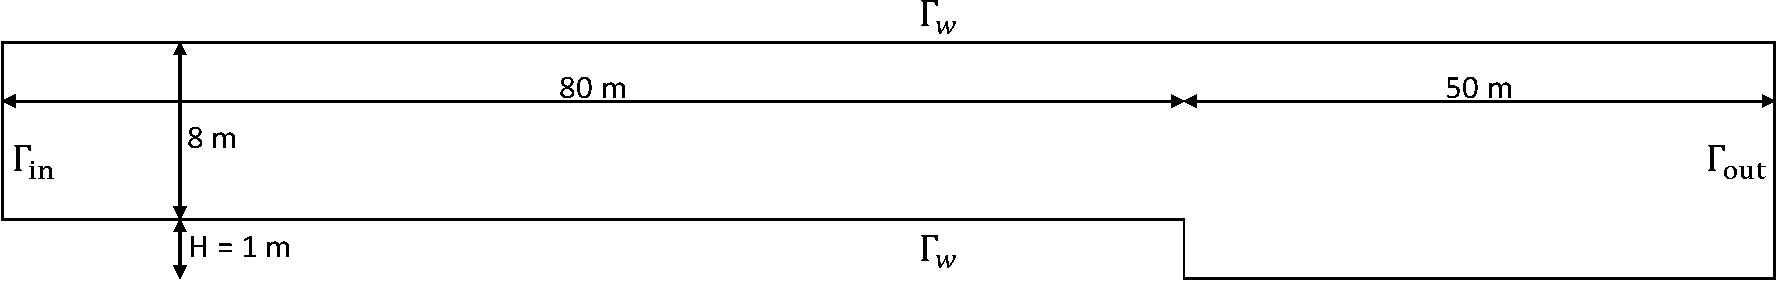
\includegraphics[width=\textwidth]{bfs_domain.pdf}
	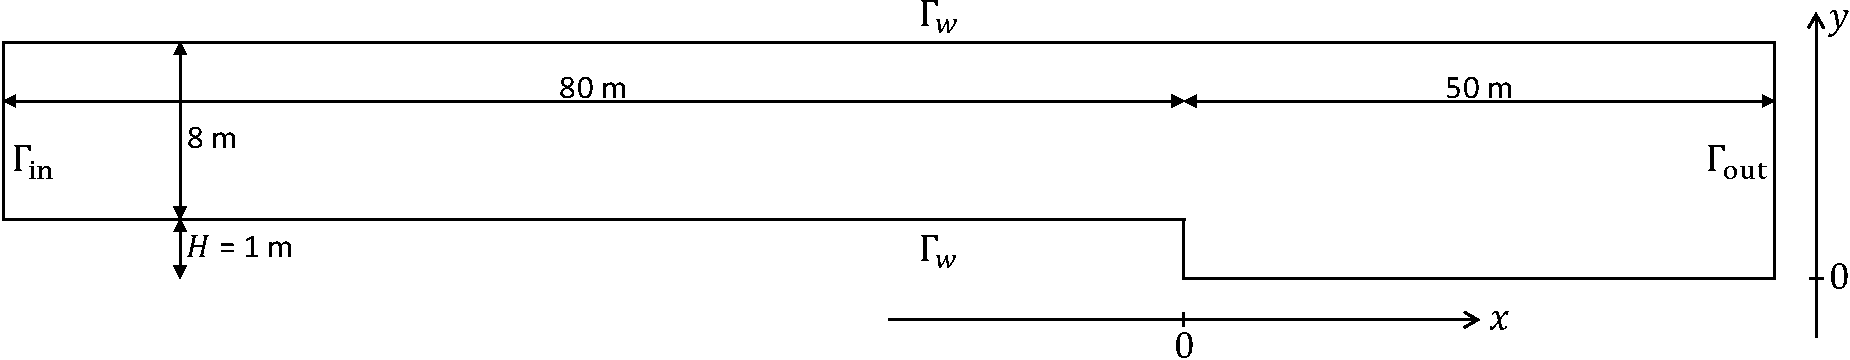
\includegraphics[width=\textwidth]{bfs_domain_axis.pdf}
	\caption[Domain of the backward facing step test]{Domain $\Omega$ of the backward facing step test. For convenience, we set the position $x=0$ at the step and the position $y=0$ at the bottom of the channel.}
	\label{fig:bfsdomain}
\end{figure}
The density is $\varrho = \SI{1}{kg/m^3}$ and the viscosity is $\nu=\SI{1.228e-3}{m^2/s}$, so that, in order to match \cite{web:nasa}, the Reynolds number based on the step height results
\begin{equation}
	Re_H = \frac{u_\text{in}H}{\nu} \simeq \num{3.6e4}.
\end{equation}

The domain sizes are chosen according to \cite{web:nasa}, with the only exception of the channel length before the step. Indeed, in \cite{web:nasa}, a small portion of the horizontal boundary near $\Gamma_\text{in}$ uses symmetry boundary conditions, but we simplify the model employing no-slip boundary conditions on the whole horizontal boundaries. As a consequence, we shorten the channel length in order to match as good as possible the profile of the $u$ component of the velocity along the section at the position $x/H=-4$, with a boundary layer thickness of approximately $1.5H$ (see Figure~\ref{fig:bfscomp}).

According to \cite{web:nasa}, CFL3D is a code for compressible fluids, but it was used at ``essentially incompressible'' conditions, such that the influence of compressibility should be very small. Moreover it is reported that, running unsteady simulations, the solution settles down and becomes reasonably steady (quasi-steady); in \cite{bfs:cfl3d} it is explained that implicit methods for ad advancement in time are used.

Thus we employ the BDF2 method for non-constant time-steps \eqref{eq:bdf2gen}, starting from $\Delta t = \SI{e-5}{s}$ and simulating until $T_\text{end} = \SI{30}{s}$. It can be observed that after approximately $t=\SI{20}{s}$ the solution stabilizes at a steady state. As initial conditions we set
\begin{equation}
p=p_\text{ext} \quad \forall \mathbf{x} \in \Omega, \quad \mathbf{v} = [u_\text{init},0]^\mathrm{T} \quad u_\text{init} = \begin{cases}
u_\text{in} \quad&\text{if $x\leq 0$}\\
\frac{8}{9}u_\text{in} \quad&\text{if $x>0$}
\end{cases}
\end{equation}
The factor $8/9$ ensures that the discharge at $\Gamma_\text{in}$ and at $\Gamma_\text{out}$ is the same. For $k$ and $\omega$ we set in the whole domain the values estimated with \eqref{eq:koic}.

According to \cite{web:nasa}, a key indicator for the reliability of a simulation is the prediction of the \emph{reattachment length} $l_\text{rea}$, i.e. the distance after the step at which the recirculation finishes and thus the $u$ component of the velocity at the bottom of the channel becomes positive. We analyse this length computing the \emph{friction coefficient} $C_f$, that is a non-dimensional form of the stress at the wall, and it is defined by:
\begin{equation}
C_f = \frac{\tau_w}{\frac{1}{2}\varrho U_\text{ref}^2}, \quad \tau_w = \mu \frac{\partial u}{\partial y} \Big|_{y=0}.
\end{equation}
$U_\text{ref}$ is the $u$ component of the velocity at $x/H=-4$ and it is the characteristic value that we use to produce non-dimensional results. In our case when $C_f<0$ the flow is recirculating, then at $x=l_{rea}$ it becomes positive. The numerical results from \cite{web:nasa} predict $l_\text{rea}/H \simeq 6.8$, while the experimental results from \cite{bfs:driver} predict $l_\text{rea}/H = 6.26 \pm 0.10$, as it can be seen in Figure~\ref{fig:bfscf}.

Performing a sensitivity analysis in order to choose a suitable grid, we observed that
\begin{itemize}
	\item with a coarse mesh the reattachment length decreases, in particular a refinement of the smallest cell in the $y$-direction in effective.
	\item too stretched cells increase the number of Newton iteration needed to get the convergence of the problem.
	\item the cells in portion of the channel after the step can be coarsened in the $x$-direction without a great influence on the solution.
	\item too refined cells in the $y$-direction in the area with the recirculation do not improve in a relevant way the solution.
\end{itemize}
So, for the following analysis, we choose a grid made of $\num{119x70}$ cells, employing gradings up to 1.25 in order to have small cells near the walls.

\begin{figure}[p] %mettere in paraview frecce 2d
	\centering
	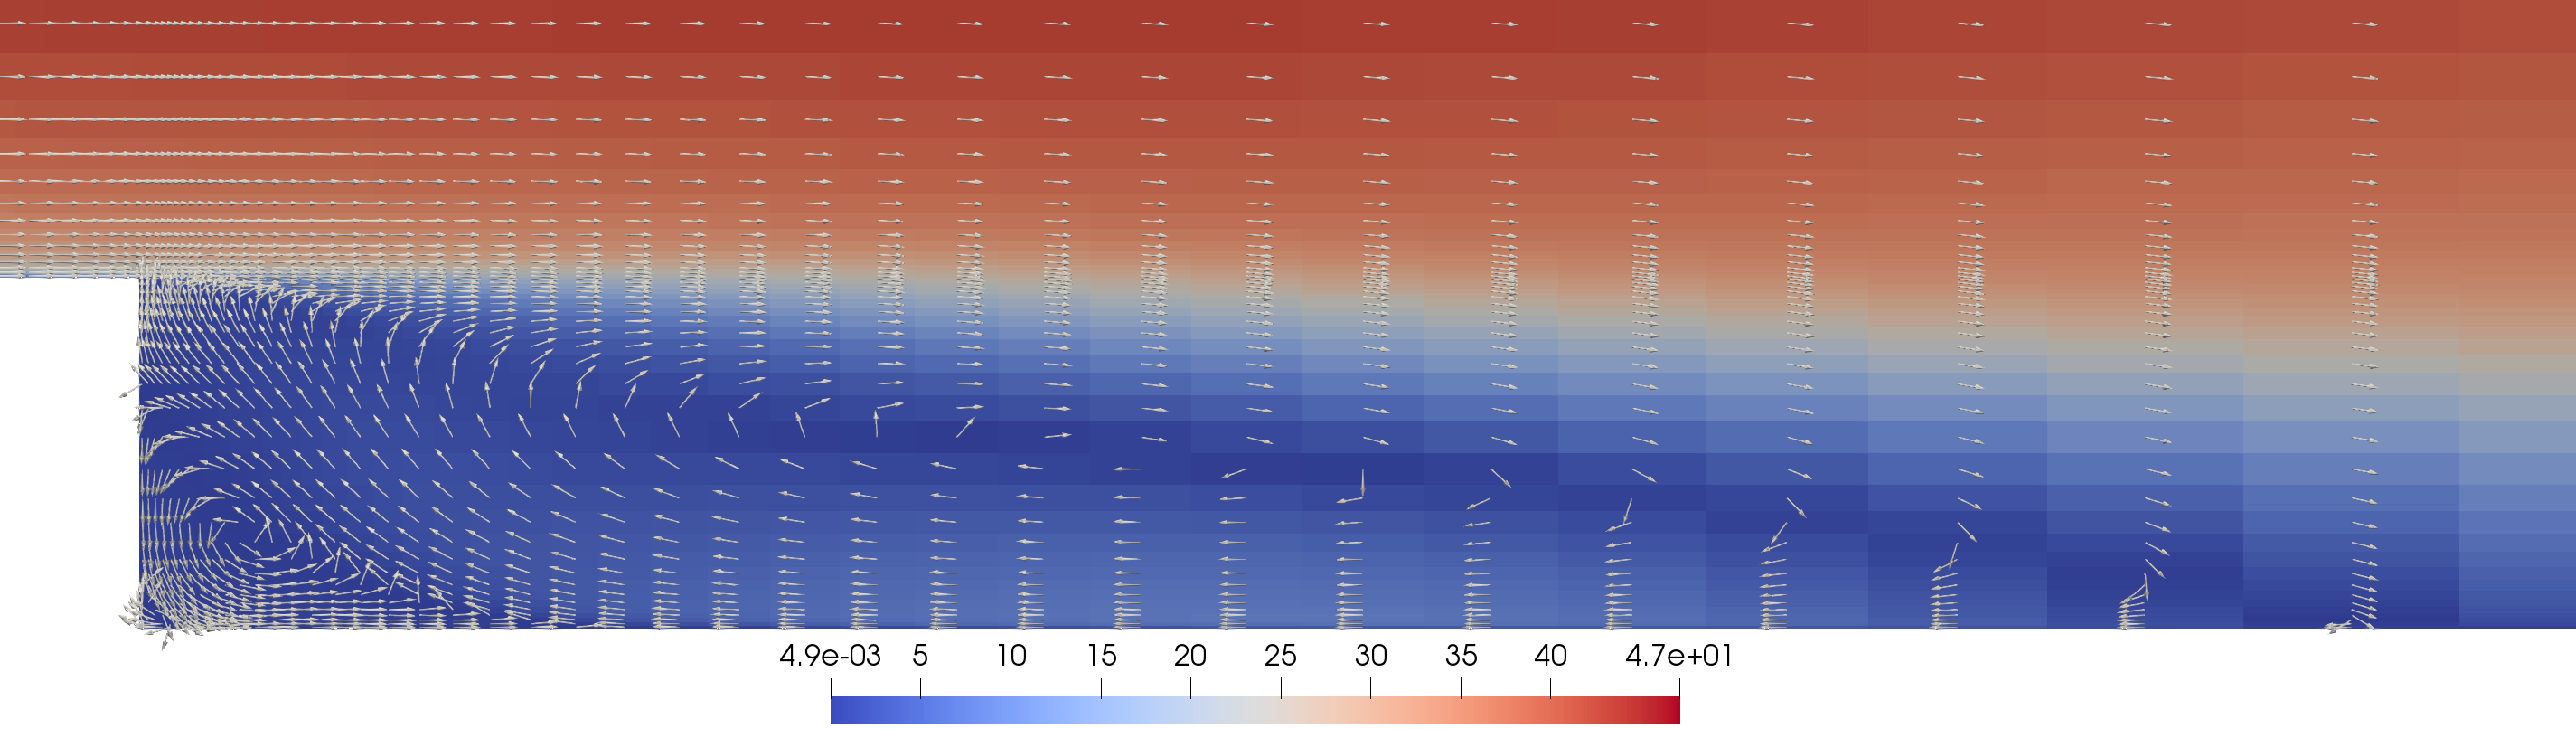
\includegraphics[width=\textwidth]{bfs_glimphs2.png}
	\caption[Velocity field after the backward facing step]{Velocity field $[\si{m/s}]$ after the backward facing step. $Re_H=\num{3.6e4}$. The arrows are not scaled.}
	\label{fig:bfsarrows}
\end{figure}
\begin{figure}[p]
	\centering
	% This file was created by matlab2tikz.
%
\definecolor{mycolor4}{rgb}{0.00000,0.44700,0.74100}%
\definecolor{mycolor3}{rgb}{0.85000,0.32500,0.09800}%
\definecolor{mycolor2}{rgb}{0.92900,0.69400,0.12500}%
\definecolor{mycolor1}{rgb}{0.49400,0.18400,0.55600}%
%
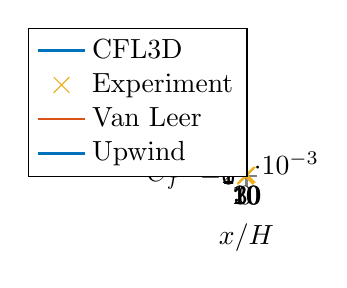
\begin{tikzpicture}

\begin{axis}[%
width=0.921\roughwidth,
height=0.75\roughwidth,
at={(0\roughwidth,0\roughwidth)},
scale only axis,
xmin=0,
xmax=30,
xlabel={$x/H$},
ymin=-0.0015,
ymax=0.0025,
ylabel style={rotate=-90},
ylabel={$C_f$},
axis background/.style={fill=white},
legend style={at={(0.97,0.03)}, anchor=south east, legend cell align=left, align=left}
]
\addplot [color=mycolor1, line width=1.0pt]
  table[row sep=crcr]{%
-0.0208296124	0.00578542007\\
0.020833334	-4.52145832e-06\\
0.0416666679	-3.42311e-06\\
0.0625	-2.00077451e-07\\
0.0833333358	3.064677e-06\\
0.104166664	6.23515825e-06\\
0.125	9.51022503e-06\\
0.145833328	1.28798602e-05\\
0.166666672	1.63185905e-05\\
0.1875	1.97527006e-05\\
0.208333328	2.31022077e-05\\
0.229166672	2.62824415e-05\\
0.25	2.92147524e-05\\
0.270833343	3.183015e-05\\
0.291666657	3.40725564e-05\\
0.3125	3.59014593e-05\\
0.333333343	3.72919931e-05\\
0.354166657	3.82353537e-05\\
0.375	3.87377113e-05\\
0.395833343	3.88185836e-05\\
0.416666657	3.85091626e-05\\
0.4375	3.78495461e-05\\
0.458333343	3.68872243e-05\\
0.479166657	3.56738892e-05\\
0.5	3.42642124e-05\\
0.520833313	3.27134367e-05\\
0.541666687	3.10765463e-05\\
0.5625	2.93949488e-05\\
0.583333313	2.7688493e-05\\
0.604166687	2.59886419e-05\\
0.625	2.43557133e-05\\
0.645833313	2.28589433e-05\\
0.666666687	2.15681812e-05\\
0.6875	2.05509914e-05\\
0.708333313	1.98652106e-05\\
0.729166687	1.95579523e-05\\
0.75	1.96612782e-05\\
0.770833313	2.01880248e-05\\
0.791666687	2.11330134e-05\\
0.8125	2.24741361e-05\\
0.833333313	2.41739781e-05\\
0.854166687	2.61832392e-05\\
0.875	2.84460075e-05\\
0.895833313	3.09032985e-05\\
0.916666687	3.34949291e-05\\
0.9375	3.61627681e-05\\
0.958333313	3.88550434e-05\\
0.979166687	4.15276518e-05\\
1	4.41418997e-05\\
1.02083337	4.66661986e-05\\
1.04166663	4.90807761e-05\\
1.0625	5.13741543e-05\\
1.08333337	5.35380932e-05\\
1.10416663	5.55709266e-05\\
1.125	5.74828264e-05\\
1.14583337	5.92902179e-05\\
1.16666663	6.09998388e-05\\
1.1875	6.26017063e-05\\
1.20833337	6.4070824e-05\\
1.22916663	6.53640236e-05\\
1.25	6.64146573e-05\\
1.27083337	6.71293965e-05\\
1.29166663	6.7386005e-05\\
1.3125	6.70321242e-05\\
1.33333337	6.58876452e-05\\
1.35416663	6.37520934e-05\\
1.375	6.04171473e-05\\
1.39583337	5.56824234e-05\\
1.41666663	4.9373255e-05\\
1.4375	4.13576272e-05\\
1.45833337	3.15600082e-05\\
1.47916663	1.99701608e-05\\
1.5	6.6458897e-06\\
1.52083337	-8.28979046e-06\\
1.54166663	-2.46563213e-05\\
1.5625	-4.22275407e-05\\
1.58333337	-6.07469265e-05\\
1.60416663	-7.99442714e-05\\
1.625	-9.95522205e-05\\
1.64583337	-0.000119321041\\
1.66666663	-0.000139030541\\
1.6875	-0.000158498267\\
1.70833337	-0.000177583803\\
1.72916663	-0.000196188877\\
1.75	-0.000214254105\\
1.77083337	-0.000231753453\\
1.79166663	-0.000248687546\\
1.8125	-0.000265076727\\
1.83333337	-0.000280954264\\
1.85416663	-0.000296360726\\
1.875	-0.000311339449\\
1.89583337	-0.000325933564\\
1.91666663	-0.000340183906\\
1.9375	-0.000354128017\\
1.95833337	-0.000367799483\\
1.97916663	-0.000381228165\\
2	-0.000394440343\\
2.02083325	-0.000407459156\\
2.04166675	-0.000420304859\\
2.0625	-0.000432995177\\
2.08333325	-0.000445545651\\
2.10416675	-0.000457969873\\
2.125	-0.000470279716\\
2.14583325	-0.000482485397\\
2.16666675	-0.000494595675\\
2.1875	-0.00050661806\\
2.20833325	-0.000518559013\\
2.22916675	-0.000530423771\\
2.25	-0.000542216934\\
2.27083325	-0.000553941994\\
2.29166675	-0.000565602095\\
2.3125	-0.000577199622\\
2.33333325	-0.000588736671\\
2.35416675	-0.00060021464\\
2.375	-0.000611634809\\
2.39583325	-0.000622998108\\
2.41666675	-0.000634305296\\
2.4375	-0.000645556778\\
2.45833325	-0.000656752964\\
2.47916675	-0.00066789391\\
2.5	-0.000678979675\\
2.52083325	-0.000690010027\\
2.54166675	-0.000700984732\\
2.5625	-0.000711903209\\
2.58333325	-0.000722764933\\
2.60416675	-0.000733568973\\
2.625	-0.00074431434\\
2.64583325	-0.00075499987\\
2.66666675	-0.000765624165\\
2.6875	-0.000776185654\\
2.70833325	-0.000786682649\\
2.72916675	-0.000797113054\\
2.75	-0.000807474891\\
2.77083325	-0.000817765831\\
2.79166675	-0.000827983546\\
2.8125	-0.000838125416\\
2.83333325	-0.000848188938\\
2.85416675	-0.000858171319\\
2.875	-0.000868069939\\
2.89583325	-0.000877882005\\
2.91666675	-0.00088760478\\
2.9375	-0.000897235645\\
2.95833325	-0.000906771864\\
2.97916675	-0.000916210993\\
3	-0.000925550528\\
3.02083325	-0.000934788026\\
3.04166675	-0.000943921274\\
3.0625	-0.000952948001\\
3.08333325	-0.000961866172\\
3.10416675	-0.000970673631\\
3.125	-0.000979368459\\
3.14583325	-0.000987948733\\
3.16666675	-0.000996412593\\
3.1875	-0.00100475841\\
3.20833325	-0.0010129842\\
3.22916675	-0.00102108845\\
3.25	-0.0010290693\\
3.27083325	-0.00103692524\\
3.29166675	-0.00104465452\\
3.3125	-0.00105225539\\
3.33333325	-0.00105972611\\
3.35416675	-0.00106706505\\
3.375	-0.00107427035\\
3.39583325	-0.00108134025\\
3.41666675	-0.00108827266\\
3.4375	-0.00109506585\\
3.45833325	-0.00110171793\\
3.47916675	-0.00110822672\\
3.5	-0.00111459021\\
3.52083325	-0.00112080644\\
3.54166675	-0.00112687331\\
3.5625	-0.00113278872\\
3.58333325	-0.00113855058\\
3.60416675	-0.00114415679\\
3.625	-0.00114960549\\
3.64583325	-0.00115489447\\
3.66666675	-0.00116002187\\
3.6875	-0.0011649857\\
3.70833325	-0.00116978423\\
3.72916675	-0.00117441558\\
3.75	-0.00117887824\\
3.77083325	-0.00118317036\\
3.79166675	-0.00118729053\\
3.8125	-0.00119123724\\
3.83333325	-0.00119500922\\
3.85416675	-0.00119860494\\
3.875	-0.00120202336\\
3.89583325	-0.00120526319\\
3.91666675	-0.00120832329\\
3.9375	-0.0012112027\\
3.95833325	-0.0012139004\\
3.97916675	-0.0012164152\\
4	-0.0012187463\\
4.02083349	-0.00122089253\\
4.04166651	-0.0012228532\\
4.0625	-0.00122462725\\
4.08333349	-0.00122621353\\
4.10416651	-0.00122761144\\
4.125	-0.00122881972\\
4.14583349	-0.00122983754\\
4.16666651	-0.00123066397\\
4.1875	-0.00123129797\\
4.20833349	-0.0012317386\\
4.22916651	-0.00123198493\\
4.25	-0.00123203604\\
4.27083349	-0.00123189087\\
4.29166651	-0.00123154873\\
4.3125	-0.00123100856\\
4.33333349	-0.00123026955\\
4.35416651	-0.00122933101\\
4.375	-0.00122819201\\
4.39583349	-0.00122685195\\
4.41666651	-0.00122531026\\
4.4375	-0.00122356624\\
4.45833349	-0.00122161943\\
4.47916651	-0.00121946924\\
4.5	-0.00121711555\\
4.52083349	-0.00121455779\\
4.54166651	-0.00121179584\\
4.5625	-0.00120882946\\
4.58333349	-0.00120565866\\
4.60416651	-0.00120228331\\
4.625	-0.00119870342\\
4.64583349	-0.00119491923\\
4.66666651	-0.00119093072\\
4.6875	-0.00118673826\\
4.70833349	-0.00118234218\\
4.72916651	-0.00117774261\\
4.75	-0.00117294013\\
4.77083349	-0.0011679352\\
4.79166651	-0.00116272818\\
4.8125	-0.00115731987\\
4.83333349	-0.00115171087\\
4.85416651	-0.00114590186\\
4.875	-0.00113989355\\
4.89583349	-0.00113368686\\
4.91666651	-0.00112728262\\
4.9375	-0.00112068199\\
4.95833349	-0.0011138859\\
4.97916651	-0.00110689562\\
5	-0.00109971222\\
5.02083349	-0.00109233696\\
5.04166651	-0.00108477136\\
5.0625	-0.0010770167\\
5.08333349	-0.00106907473\\
5.10416651	-0.00106094684\\
5.125	-0.00105263491\\
5.14583349	-0.00104414055\\
5.16666651	-0.00103546574\\
5.1875	-0.00102661236\\
5.20833349	-0.00101758237\\
5.22916651	-0.00100837788\\
5.25	-0.000999001088\\
5.27083349	-0.000989454216\\
5.29166651	-0.000979739358\\
5.3125	-0.000969859073\\
5.33333349	-0.000959815574\\
5.35416651	-0.000949611305\\
5.375	-0.000939248886\\
5.39583349	-0.000928730704\\
5.41666651	-0.000918059377\\
5.4375	-0.000907237467\\
5.45833349	-0.000896267651\\
5.47916651	-0.000885152607\\
5.5	-0.000873894955\\
5.52083349	-0.000862497487\\
5.54166651	-0.000850962882\\
5.5625	-0.000839293993\\
5.58333349	-0.000827493554\\
5.60416651	-0.000815564359\\
5.625	-0.000803509203\\
5.64583349	-0.000791331055\\
5.66666651	-0.000779032591\\
5.6875	-0.000766616839\\
5.70833349	-0.00075408665\\
5.72916651	-0.000741444877\\
5.75	-0.000728694431\\
5.77083349	-0.00071583828\\
5.79166651	-0.000702879392\\
5.8125	-0.000689820619\\
5.83333349	-0.000676664989\\
5.85416651	-0.000663415354\\
5.875	-0.000650074857\\
5.89583349	-0.000636646291\\
5.91666651	-0.000623132684\\
5.9375	-0.000609537063\\
5.95833349	-0.000595862279\\
5.97916651	-0.000582111359\\
6	-0.000568287272\\
6.02083349	-0.000554392929\\
6.04166651	-0.000540431298\\
6.0625	-0.000526405289\\
6.08333349	-0.000512317813\\
6.10416651	-0.000498171838\\
6.125	-0.000483970158\\
6.14583349	-0.000469715713\\
6.16666651	-0.000455411355\\
6.1875	-0.000441059936\\
6.20833349	-0.000426664308\\
6.22916651	-0.000412227295\\
6.25	-0.00039775169\\
6.27083349	-0.000383240316\\
6.29166651	-0.00036869591\\
6.3125	-0.000354121235\\
6.33333349	-0.000339519058\\
6.35416651	-0.000324892113\\
6.375	-0.000310243078\\
6.39583349	-0.00029557466\\
6.41666651	-0.000280889537\\
6.4375	-0.000266190385\\
6.45833349	-0.000251479767\\
6.47916651	-0.000236760374\\
6.5	-0.000222034723\\
6.52083349	-0.00020730542\\
6.54166651	-0.000192574982\\
6.5625	-0.000177845926\\
6.58333349	-0.000163120698\\
6.60416651	-0.000148401756\\
6.625	-0.00013369153\\
6.64583349	-0.000118992386\\
6.66666651	-0.000104306666\\
6.6875	-8.9636691e-05\\
6.70833349	-7.49847459e-05\\
6.72916651	-6.03530607e-05\\
6.75	-4.57438473e-05\\
6.77083349	-3.11592739e-05\\
6.79166651	-1.66014652e-05\\
6.8125	-2.07251423e-06\\
6.83333349	1.24255303e-05\\
6.85416651	2.68906606e-05\\
6.875	4.13209091e-05\\
6.89583349	5.57143467e-05\\
6.91666651	7.00690798e-05\\
6.9375	8.4383275e-05\\
6.95833349	9.86551095e-05\\
6.97916651	0.00011288283\\
7	0.000127064704\\
7.02083349	0.000141199023\\
7.04166651	0.000155284171\\
7.0625	0.000169318519\\
7.08333349	0.000183300508\\
7.10416651	0.000197228583\\
7.125	0.000211101244\\
7.14583349	0.00022491705\\
7.16666651	0.000238674562\\
7.1875	0.000252372382\\
7.20833349	0.000266009156\\
7.22916651	0.000279583532\\
7.25	0.000293094228\\
7.27083349	0.000306539936\\
7.29166651	0.000319919433\\
7.3125	0.000333231408\\
7.33333349	0.00034647467\\
7.35416651	0.000359647966\\
7.375	0.000372750073\\
7.39583349	0.000385779713\\
7.41666651	0.000398735632\\
7.4375	0.000411616522\\
7.45833349	0.000424421014\\
7.47916651	0.000437147653\\
7.5	0.000449794927\\
7.52083349	0.000462361146\\
7.54166651	0.000474844506\\
7.5625	0.000487243\\
7.58333349	0.000499554328\\
7.60416651	0.000511775957\\
7.625	0.000523904979\\
7.64583349	0.000535938016\\
7.66666651	0.000547871226\\
7.6875	0.000559699663\\
7.70833349	0.000571417506\\
7.72916651	0.000583016896\\
7.75	0.000594487821\\
7.77083349	0.00060581672\\
7.79166651	0.000616987527\\
7.8125	0.000627978356\\
7.83333349	0.000638775527\\
7.85416651	0.000649344816\\
7.875	0.000659732206\\
7.89583349	0.000669804227\\
7.91666651	0.000679981546\\
7.9375	0.000689163571\\
7.95833349	0.000700129895\\
7.97916651	0.000703911763\\
8.02083778	0.000720021199\\
8.04170799	0.000736109505\\
8.06264305	0.000746689155\\
8.08367729	0.000759218005\\
8.10484314	0.00077105721\\
8.12617397	0.000783165509\\
8.14770222	0.000795124448\\
8.16946316	0.000807045843\\
8.19149113	0.000818875851\\
8.2138195	0.000830641133\\
8.23648357	0.000842353154\\
8.25951958	0.000854035665\\
8.28296375	0.000865710492\\
8.30685234	0.000877400045\\
8.33122349	0.000889124814\\
8.35611534	0.000900904008\\
8.38156605	0.000912755087\\
8.40761757	0.000924694061\\
8.43430901	0.000936735712\\
8.46168327	0.000948893605\\
8.48978329	0.000961180194\\
8.51865292	0.000973607064\\
8.54833794	0.000986184808\\
8.57888508	0.000998923322\\
8.61034203	0.00101183145\\
8.64275837	0.00102491723\\
8.67618465	0.00103818811\\
8.71067333	0.00105165015\\
8.74627972	0.00106530928\\
8.78305912	0.0010791698\\
8.82106876	0.00109323568\\
8.86036873	0.0011075096\\
8.90102196	0.00112199329\\
8.94309044	0.00113668793\\
8.98664188	0.00115159305\\
9.031744	0.00116670749\\
9.07846737	0.00118202891\\
9.12688637	0.00119755394\\
9.17707634	0.00121327781\\
9.22911549	0.00122919504\\
9.28308773	0.00124529866\\
9.33907604	0.00126158085\\
9.39716911	0.00127803243\\
9.4574585	0.0012946428\\
9.5200386	0.00131140009\\
9.58500767	0.00132829195\\
9.65246773	0.00134530477\\
9.7225256	0.00136242353\\
9.79529095	0.00137963158\\
9.87087727	0.00139691227\\
9.94940472	0.00141424872\\
10.0309963	0.00143162115\\
10.1157799	0.00144901045\\
10.2038889	0.00146639836\\
10.2954617	0.00148376392\\
10.3906431	0.00150108722\\
10.4895811	0.0015183494\\
10.592433	0.00153552997\\
10.6993589	0.00155261008\\
10.8105278	0.00156957074\\
10.9261141	0.00158639357\\
11.0462999	0.0016030618\\
11.1712732	0.00161955832\\
11.3012314	0.0016358674\\
11.4363775	0.00165197439\\
11.5769253	0.0016678652\\
11.7230959	0.00168352807\\
11.8751173	0.0016989531\\
12.0332298	0.00171413017\\
12.1976814	0.00172905205\\
12.3687305	0.00174371328\\
12.5466471	0.00175810675\\
12.7317095	0.00177222933\\
12.9242086	0.00178607856\\
13.1244478	0.00179964968\\
13.3327408	0.00181294058\\
13.5494156	0.00182595244\\
13.7748137	0.00183868664\\
14.0092878	0.00185114262\\
14.2532063	0.00186331989\\
14.5069542	0.00187521882\\
14.7709293	0.00188683881\\
15.0455465	0.00189817743\\
15.3312378	0.00190922979\\
15.6284523	0.00191998936\\
15.9376564	0.00193044927\\
16.2593365	0.00194060185\\
16.593998	0.00195043813\\
16.9421673	0.0019599488\\
17.3043919	0.00196912582\\
17.6812401	0.00197796384\\
18.073307	0.00198646192\\
18.481205	0.00199462124\\
18.9055767	0.00200244761\\
19.3470898	0.00200995617\\
19.8064365	0.00201716716\\
20.2843418	0.00202410598\\
20.7815533	0.0020308001\\
21.2988548	0.00203728001\\
21.8370609	0.00204357714\\
22.3970127	0.00204972457\\
22.9795952	0.00205575\\
23.5857201	0.00206167158\\
24.2163429	0.00206749956\\
24.8724537	0.0020732386\\
25.5550842	0.0020788915\\
26.2653065	0.00208445569\\
27.0042381	0.00208992814\\
27.7730389	0.00209530792\\
28.5729198	0.0021005962\\
29.4051342	0.00210579601\\
30.2709942	0.00211091153\\
31.1718578	0.00211594626\\
32.1091423	0.00212090067\\
33.0843201	0.00212577032\\
34.0989227	0.00213054521\\
35.1545486	0.00213520718\\
36.2528534	0.00213972898\\
37.395565	0.00214405521\\
38.5844803	0.00214811601\\
39.8214684	0.00215172442\\
41.1084671	0.00215476262\\
42.4475098	0.00215645414\\
43.8406906	0.00215760223\\
45.2902069	0.0021544348\\
46.798336	0.00215237797\\
48.3674431	0.00214179186\\
};
\addlegendentry{CFL3D}

\addplot [color=mycolor2, draw=none, mark=x, mark size=4pt, mark options={solid, mycolor2}, only marks]
  table[row sep=crcr]{%
-3.956	0.00288\\
-1.804	0.00285\\
-0.804	0.00311\\
0.484	9e-05\\
1.804	-0.00011\\
2.804	-0.00052\\
3.804	-0.00102\\
4.804	-0.00082\\
5.882	-0.00022\\
7.09	0.00045\\
7.978	0.00102\\
9.196	0.00118\\
11.196	0.00154\\
13.196	0.00173\\
16.196	0.00191\\
20.196	0.00202\\
24.136	0.00204\\
28.13	0.00205\\
32.196	0.00212\\
35.994	0.0023\\
};
\addlegendentry{Experiment}

\addplot [color=mycolor3, line width=1.0pt]
  table[row sep=crcr]{%
0	0\\
0.05	-2.73642133427827e-06\\
0.1	8.60199744470485e-07\\
0.15	1.63031249997315e-05\\
0.2	3.14838415922525e-05\\
0.25	4.07366468242058e-05\\
0.3	4.37922492100848e-05\\
0.35	4.26059031041435e-05\\
0.4	3.95874241105936e-05\\
0.45	3.66285027896292e-05\\
0.5	3.52610799930467e-05\\
0.55	3.60409383067227e-05\\
0.6	3.88150438903365e-05\\
0.65	4.42444067871579e-05\\
0.7	5.08983074813096e-05\\
0.75	5.82407269195218e-05\\
0.8	6.54942104610032e-05\\
0.85	7.23842052473773e-05\\
0.9	7.7101279746057e-05\\
0.95	8.11437233884541e-05\\
1	8.05628357746715e-05\\
1.05	7.99819481608889e-05\\
1.1	6.96490925794473e-05\\
1.15	5.8358773965633e-05\\
1.2	3.96306902225167e-05\\
1.25	1.25891566107557e-05\\
1.3	-1.44524304159583e-05\\
1.35	-5.06798403235744e-05\\
1.4	-8.93519992146586e-05\\
1.45	-0.000128024158105743\\
1.5	-0.000167843937261849\\
1.55	-0.000207883518949516\\
1.6	-0.000247922833562418\\
1.65	-0.000285088957853907\\
1.7	-0.000320286741127658\\
1.75	-0.00035548452440141\\
1.8	-0.000390562124030931\\
1.85	-0.000420570644621558\\
1.9	-0.000450579165212185\\
1.95	-0.000480587685802812\\
2	-0.000510254350694294\\
2.05	-0.000536708106163337\\
2.1	-0.000563161861632379\\
2.15	-0.000589612946353772\\
2.2	-0.000616066701822814\\
2.25	-0.000640690995151898\\
2.3	-0.000664789151194015\\
2.35	-0.000688884636488483\\
2.4	-0.0007129827925306\\
2.45	-0.000737032875115025\\
2.5	-0.000759234800325944\\
2.55	-0.000781436725536863\\
2.6	-0.000803638650747781\\
2.65	-0.00082584324670635\\
2.7	-0.000848045171917268\\
2.75	-0.000868358878539938\\
2.8	-0.000888194521333333\\
2.85	-0.000908030164126728\\
2.9	-0.000927865806920123\\
2.95	-0.000947701449713518\\
3	-0.000967371506152639\\
3.05	-0.000983711140272741\\
3.1	-0.00100004810364519\\
3.15	-0.00101638773776529\\
3.2	-0.00103272737188539\\
3.25	-0.0010490670060055\\
3.3	-0.0010654066401256\\
3.35	-0.0010779324466021\\
3.4	-0.00108899735411429\\
3.45	-0.00110006226162648\\
3.5	-0.00111112983988632\\
3.55	-0.00112219474739852\\
3.6	-0.00113325965491071\\
3.65	-0.00114432723317054\\
3.7	-0.0011496153135167\\
3.75	-0.00115313802966649\\
3.8	-0.00115666074581628\\
3.85	-0.00116018346196607\\
3.9	-0.00116370884886351\\
3.95	-0.0011672315650133\\
4	-0.00117075428116309\\
4.05	-0.00117324074722485\\
4.1	-0.00116759745744129\\
4.15	-0.00116195416765774\\
4.2	-0.00115631087787419\\
4.25	-0.00115066758809064\\
4.3	-0.00114502429830708\\
4.35	-0.00113938100852353\\
4.4	-0.00113373771873998\\
4.45	-0.00112809442895643\\
4.5	-0.00111578762378718\\
4.55	-0.00110055902068931\\
4.6	-0.00108533041759143\\
4.65	-0.00107010181449355\\
4.7	-0.00105487054064802\\
4.75	-0.00103964193755014\\
4.8	-0.00102441333445227\\
4.85	-0.00100918473135439\\
4.9	-0.000993956128256511\\
4.95	-0.000975049905645168\\
5	-0.000951371056984034\\
5.05	-0.0009276922083229\\
5.1	-0.000904010688914117\\
5.15	-0.000880331840252983\\
5.2	-0.000856652991591849\\
5.25	-0.000832971472183066\\
5.3	-0.000809292623521932\\
5.35	-0.000785613774860798\\
5.4	-0.000761934926199664\\
5.45	-0.000736902008480196\\
5.5	-0.000707790859099826\\
5.55	-0.000678679709719456\\
5.6	-0.000649568560339086\\
5.65	-0.000620457410958716\\
5.7	-0.000591346261578346\\
5.75	-0.000562235112197977\\
5.8	-0.000533123962817607\\
5.85	-0.000504012813437237\\
5.9	-0.000474901664056867\\
5.95	-0.000445790514676497\\
6	-0.000416612596604888\\
6.05	-0.000385987133307209\\
6.1	-0.00035535899926188\\
6.15	-0.000324733535964201\\
6.2	-0.000294105401918873\\
6.25	-0.000263480205695958\\
6.3	-0.000232853407024455\\
6.35	-0.000202227142502481\\
6.4	-0.000171600610905742\\
6.45	-0.000140974346383768\\
6.5	-0.000110347814787029\\
6.55	-7.97210161155254e-05\\
6.6	-4.90947515935515e-05\\
6.65	-1.98156121860233e-05\\
6.7	8.93728310463253e-06\\
6.75	3.76903920551003e-05\\
6.8	6.64436612504271e-05\\
6.85	9.5196396296224e-05\\
6.9	0.000123949665491551\\
6.95	0.000152702667612113\\
7	0.000181455669732674\\
7.05	0.000210208938928001\\
7.1	0.000238961941048563\\
7.15	0.00026771574439342\\
7.2	0.000296469013588747\\
7.25	0.000325222282784073\\
7.3	0.000353273145347562\\
7.35	0.00037767843736938\\
7.4	0.000402086400138848\\
7.45	0.000426494362908316\\
7.5	0.000450902325677784\\
7.55	0.000475310288447252\\
7.6	0.00049971825121672\\
7.65	0.000524126213986188\\
7.7	0.000548534176755656\\
7.75	0.000572942139525124\\
7.8	0.000597350102294591\\
7.85	0.000621758065064059\\
7.9	0.000646166027833527\\
7.95	0.000670573990602995\\
8	0.000694981953372463\\
8.05	0.0007180144811024\\
8.1	0.000736885983994298\\
8.15	0.000755757486886197\\
8.2	0.000774628989778095\\
8.25	0.000793503163417643\\
8.3	0.000812374666309542\\
8.35	0.00083124616920144\\
8.4	0.000850117672093339\\
8.45	0.000868989174985237\\
8.5	0.000887863348624785\\
8.55	0.000906734851516684\\
8.6	0.000925606354408582\\
8.65	0.000944477857300481\\
8.7	0.000963349360192379\\
8.75	0.000982223533831927\\
8.8	0.00100109503672383\\
8.85	0.00101996653961572\\
8.9	0.00103434851570869\\
8.95	0.00104789988928263\\
9	0.00106145126285658\\
9.05	0.00107500263643052\\
9.1	0.00108855401000447\\
9.15	0.00110210538357841\\
9.2	0.00111565675715235\\
9.25	0.0011292081307263\\
9.3	0.00114275950430024\\
9.35	0.00115631087787419\\
9.4	0.00116986225144813\\
9.45	0.00118341362502208\\
9.5	0.00119696499859602\\
9.55	0.00121051637216997\\
9.6	0.00122406774574391\\
9.65	0.00123761911931786\\
9.7	0.0012511704928918\\
9.75	0.00126472186646575\\
9.8	0.00127482530482409\\
9.85	0.00128405807944867\\
9.9	0.0012932935248209\\
9.95	0.00130252629944548\\
10	0.00131176174481771\\
10.05	0.0013209945194423\\
10.1	0.00133022996481453\\
10.15	0.00133946273943911\\
10.2	0.00134869818481134\\
10.25	0.00135793095943592\\
10.3	0.00136716640480815\\
10.35	0.00137639917943273\\
10.4	0.00138563462480496\\
10.45	0.00139486739942955\\
10.5	0.00140410284480178\\
10.55	0.00141333561942636\\
10.6	0.00142257106479859\\
10.65	0.00143180383942317\\
10.7	0.0014410392847954\\
10.75	0.00145027205941998\\
10.8	0.00145654297490119\\
10.85	0.00146265364552341\\
10.9	0.00146876164539799\\
10.95	0.00147487231602022\\
11	0.0014809803158948\\
11.05	0.00148709098651703\\
11.1	0.00149319898639161\\
11.15	0.00149930965701383\\
11.2	0.00150541765688841\\
11.25	0.00151152565676299\\
11.3	0.00151763632738522\\
11.35	0.0015237443272598\\
11.4	0.00152985499788203\\
11.45	0.0015359629977566\\
11.5	0.00154207366837883\\
11.55	0.00154818166825341\\
11.6	0.00155429233887564\\
11.65	0.00156040033875022\\
11.7	0.0015665083386248\\
11.75	0.00157261900924702\\
11.8	0.0015787270091216\\
11.85	0.00158459731245537\\
11.9	0.00158861678766798\\
11.95	0.00159263359213294\\
12	0.0015966503965979\\
12.05	0.00160066720106286\\
12.1	0.00160468400552782\\
12.15	0.00160870080999279\\
12.2	0.00161271761445775\\
12.25	0.00161673708967036\\
12.3	0.00162075389413532\\
12.35	0.00162477069860028\\
12.4	0.00162878750306524\\
12.45	0.0016328043075302\\
12.5	0.00163682111199516\\
12.55	0.00164083791646012\\
12.6	0.00164485739167274\\
12.65	0.0016488741961377\\
12.7	0.00165289100060266\\
12.75	0.00165690780506762\\
12.8	0.00166092460953258\\
12.85	0.00166494141399754\\
12.9	0.0016689582184625\\
12.95	0.00167297769367511\\
13	0.00167699449814007\\
13.05	0.00168088310671786\\
13.1	0.00168355919586273\\
13.15	0.00168623795575525\\
13.2	0.00168891404490013\\
13.25	0.001691590134045\\
13.3	0.00169426889393753\\
13.35	0.0016969449830824\\
13.4	0.00169962374297493\\
13.45	0.0017022998321198\\
13.5	0.00170497859201232\\
13.55	0.0017076546811572\\
13.6	0.00171033077030207\\
13.65	0.0017130095301946\\
13.7	0.00171568561933947\\
13.75	0.00171836437923199\\
13.8	0.00172104046837687\\
13.85	0.00172371655752174\\
13.9	0.00172639531741427\\
13.95	0.00172907140655914\\
14	0.00173175016645166\\
14.05	0.00173442625559654\\
14.1	0.00173710501548906\\
14.15	0.00173978110463394\\
14.2	0.00174245719377881\\
14.25	0.00174513595367134\\
14.3	0.00174781204281621\\
14.35	0.00175049080270873\\
14.4	0.0017525900103613\\
14.45	0.00175441146025831\\
14.5	0.00175623291015532\\
14.55	0.00175805703079998\\
14.6	0.00175987848069699\\
14.65	0.001761699930594\\
14.7	0.00176352138049101\\
14.75	0.00176534550113567\\
14.8	0.00176716695103268\\
14.85	0.00176898840092969\\
14.9	0.00177081252157435\\
14.95	0.00177263397147136\\
15	0.00177445542136837\\
15.05	0.00177627687126538\\
15.1	0.00177810099191004\\
15.15	0.00177992244180705\\
15.2	0.00178174389170406\\
15.25	0.00178356801234872\\
15.3	0.00178538946224573\\
15.35	0.00178721091214274\\
15.4	0.00178903236203975\\
15.45	0.00179085648268441\\
15.5	0.00179267793258142\\
15.55	0.00179449938247843\\
15.6	0.00179632350312309\\
15.65	0.0017981449530201\\
15.7	0.00179996640291712\\
15.75	0.00180178785281413\\
15.8	0.00180361197345879\\
15.85	0.0018050942384043\\
15.9	0.0018063655142855\\
15.95	0.0018076367901667\\
16	0.00180890806604789\\
16.05	0.00181017934192909\\
16.1	0.00181145061781029\\
16.15	0.00181272189369149\\
16.2	0.00181399316957268\\
16.25	0.00181526444545388\\
16.3	0.00181653572133508\\
16.35	0.00181780699721628\\
16.4	0.00181907827309748\\
16.45	0.00182034954897867\\
16.5	0.00182162082485987\\
16.55	0.00182289210074107\\
16.6	0.00182416337662227\\
16.65	0.00182543465250346\\
16.7	0.00182670592838466\\
16.75	0.00182797720426586\\
16.8	0.00182924848014706\\
16.85	0.00183051975602826\\
16.9	0.00183179103190945\\
16.95	0.00183306230779065\\
17	0.00183433358367185\\
17.05	0.00183560485955305\\
17.1	0.00183687613543425\\
17.15	0.00183814741131544\\
17.2	0.00183941868719664\\
17.25	0.00184068996307784\\
17.3	0.00184196123895904\\
17.35	0.00184323251484023\\
17.4	0.00184450379072143\\
17.45	0.00184554538230477\\
17.5	0.00184646411949622\\
17.55	0.00184738018594002\\
17.6	0.00184829625238383\\
17.65	0.00184921231882763\\
17.7	0.00185013105601909\\
17.75	0.00185104712246289\\
17.8	0.0018519631889067\\
17.85	0.00185288192609815\\
17.9	0.00185379799254195\\
17.95	0.00185471405898576\\
18	0.00185563012542956\\
18.05	0.00185654886262102\\
18.1	0.00185746492906482\\
18.15	0.00185838099550862\\
18.2	0.00185929973270008\\
18.25	0.00186021579914388\\
18.3	0.00186113186558769\\
18.35	0.00186204793203149\\
18.4	0.00186296666922295\\
18.45	0.00186388273566675\\
18.5	0.00186479880211055\\
18.55	0.00186571753930201\\
18.6	0.00186663360574581\\
18.65	0.00186754967218962\\
18.7	0.00186846840938107\\
18.75	0.00186938447582487\\
18.8	0.00187030054226868\\
18.85	0.00187121660871248\\
18.9	0.00187213534590394\\
18.95	0.00187305141234774\\
19	0.00187396747879155\\
19.05	0.001874886215983\\
19.1	0.0018758022824268\\
19.15	0.00187671834887061\\
19.2	0.00187752758540843\\
19.25	0.00187821663830202\\
19.3	0.00187890569119561\\
19.35	0.00187959741483685\\
19.4	0.00188028646773044\\
19.45	0.00188097552062403\\
19.5	0.00188166724426527\\
19.55	0.00188235629715886\\
19.6	0.0018830480208001\\
19.65	0.00188373707369369\\
19.7	0.00188442612658728\\
19.75	0.00188511785022852\\
19.8	0.00188580690312211\\
19.85	0.00188649862676335\\
19.9	0.00188718767965694\\
19.95	0.00188787673255053\\
20	0.00188856845619177\\
20.05	0.00188925750908536\\
20.1	0.0018899492327266\\
20.15	0.00189063828562019\\
20.2	0.00189132733851378\\
20.25	0.00189201906215502\\
20.3	0.00189270811504861\\
20.35	0.00189339716794221\\
20.4	0.00189408889158345\\
20.45	0.00189477794447704\\
20.5	0.00189546966811828\\
20.55	0.00189615872101187\\
20.6	0.00189684777390546\\
20.65	0.0018975394975467\\
20.7	0.00189822855044029\\
20.75	0.00189892027408153\\
20.8	0.00189960932697512\\
20.85	0.00190029837986871\\
20.9	0.00190099010350995\\
20.95	0.00190167915640354\\
21	0.00190237088004478\\
21.05	0.00190305993293837\\
21.1	0.00190374898583196\\
21.15	0.00190432052582897\\
21.2	0.00190486535834948\\
21.25	0.00190540752012234\\
21.3	0.00190594968189521\\
21.35	0.00190649184366807\\
21.4	0.00190703400544094\\
21.45	0.0019075761672138\\
21.5	0.00190811832898666\\
21.55	0.00190866049075953\\
21.6	0.00190920265253239\\
21.65	0.00190974481430526\\
21.7	0.00191028697607812\\
21.75	0.00191082913785098\\
21.8	0.00191137129962385\\
21.85	0.00191191346139671\\
21.9	0.00191245562316957\\
21.95	0.00191300045569009\\
22	0.00191354261746295\\
22.05	0.00191408477923581\\
22.1	0.00191462694100868\\
22.15	0.00191516910278154\\
22.2	0.00191571126455441\\
22.25	0.00191625342632727\\
22.3	0.00191679558810013\\
22.35	0.001917337749873\\
22.4	0.00191787991164586\\
22.45	0.00191842207341872\\
22.5	0.00191896423519159\\
22.55	0.00191950639696445\\
22.6	0.00192004855873732\\
22.65	0.00192059072051018\\
22.7	0.00192113555303069\\
22.75	0.00192167771480356\\
22.8	0.00192221987657642\\
22.85	0.00192276203834928\\
22.9	0.00192330420012215\\
22.95	0.00192384636189501\\
23	0.00192438852366788\\
23.05	0.00192493068544074\\
23.1	0.0019254728472136\\
23.15	0.00192601500898647\\
23.2	0.00192655717075933\\
23.25	0.00192707529580335\\
23.3	0.00192751863991318\\
23.35	0.00192795931327536\\
23.4	0.00192840265738519\\
23.45	0.00192884600149502\\
23.5	0.00192928934560485\\
23.55	0.00192973001896703\\
23.6	0.00193017336307686\\
23.65	0.00193061670718669\\
23.7	0.00193105738054887\\
23.75	0.00193150072465869\\
23.8	0.00193194406876852\\
23.85	0.00193238741287835\\
23.9	0.00193282808624053\\
23.95	0.00193327143035036\\
24	0.00193371477446019\\
24.05	0.00193415544782237\\
24.1	0.0019345987919322\\
24.15	0.00193504213604203\\
24.2	0.00193548548015186\\
24.25	0.00193592615351404\\
24.3	0.00193636949762387\\
24.35	0.0019368128417337\\
24.4	0.00193725618584353\\
24.45	0.00193769685920571\\
24.5	0.00193814020331554\\
24.55	0.00193858354742537\\
24.6	0.00193902422078755\\
24.65	0.00193946756489738\\
24.7	0.00193991090900721\\
24.75	0.00194035425311704\\
24.8	0.00194079492647922\\
24.85	0.00194123827058905\\
24.9	0.00194168161469888\\
24.95	0.00194212228806105\\
25	0.00194256563217089\\
25.05	0.00194300897628071\\
25.1	0.00194345232039054\\
25.15	0.00194389299375272\\
25.2	0.00194433633786255\\
25.25	0.00194477968197238\\
25.3	0.00194522302608221\\
25.35	0.00194566369944439\\
25.4	0.00194610704355422\\
25.45	0.00194655038766405\\
25.5	0.00194699106102623\\
25.55	0.00194743440513606\\
25.6	0.00194784570027409\\
25.65	0.00194821693419739\\
25.7	0.00194859083886833\\
25.75	0.00194896207279162\\
25.8	0.00194933330671491\\
25.85	0.00194970721138585\\
25.9	0.00195007844530914\\
25.95	0.00195044967923243\\
26	0.00195082358390337\\
26.05	0.00195119481782666\\
26.1	0.00195156605174995\\
26.15	0.00195193728567324\\
26.2	0.00195231119034418\\
26.25	0.00195268242426748\\
26.3	0.00195305365819077\\
26.35	0.00195342756286171\\
26.4	0.001953798796785\\
26.45	0.00195417003070829\\
26.5	0.00195454393537923\\
26.55	0.00195491516930252\\
26.6	0.00195528640322581\\
26.65	0.00195566030789675\\
26.7	0.00195603154182004\\
26.75	0.00195640277574333\\
26.8	0.00195677400966663\\
26.85	0.00195714791433757\\
26.9	0.00195751914826086\\
26.95	0.00195789038218415\\
27	0.00195826428685509\\
27.05	0.00195863552077838\\
27.1	0.00195900675470167\\
27.15	0.00195938065937261\\
27.2	0.0019597518932959\\
27.25	0.00196012312721919\\
27.3	0.00196049436114248\\
27.35	0.00196086826581342\\
27.4	0.00196123949973672\\
27.45	0.00196161073366001\\
27.5	0.00196198463833095\\
27.55	0.00196235587225424\\
27.6	0.00196272710617753\\
27.65	0.00196310101084847\\
27.7	0.00196347224477176\\
27.75	0.00196384347869505\\
27.8	0.00196421738336599\\
27.85	0.00196458861728928\\
27.9	0.00196495985121257\\
27.95	0.00196533108513586\\
28	0.0019657049898068\\
28.05	0.0019660762237301\\
28.1	0.00196644745765339\\
28.15	0.00196682136232433\\
28.2	0.00196713918129463\\
28.25	0.00196745700026493\\
28.3	0.00196777481923523\\
28.35	0.00196809263820553\\
28.4	0.00196841045717582\\
28.45	0.00196872827614612\\
28.5	0.00196904609511642\\
28.55	0.00196936391408672\\
28.6	0.00196968173305702\\
28.65	0.00196999955202732\\
28.7	0.00197031737099762\\
28.75	0.00197063251922027\\
28.8	0.00197095033819057\\
28.85	0.00197126815716087\\
28.9	0.00197158597613117\\
28.95	0.00197190379510147\\
29	0.00197222161407177\\
29.05	0.00197253943304207\\
29.1	0.00197285725201237\\
29.15	0.00197317507098267\\
29.2	0.00197349288995297\\
29.25	0.00197381070892327\\
29.3	0.00197412585714592\\
29.35	0.00197444367611621\\
29.4	0.00197476149508651\\
29.45	0.00197507931405681\\
29.5	0.00197539713302711\\
29.55	0.00197571495199741\\
29.6	0.00197603277096771\\
29.65	0.00197635058993801\\
29.7	0.00197666840890831\\
29.75	0.00197698622787861\\
29.8	0.00197730404684891\\
29.85	0.00197762186581921\\
29.9	0.00197793701404186\\
29.95	0.00197825483301216\\
30	0.00197857265198246\\
30.05	0.00197889047095276\\
30.1	0.00197920828992306\\
30.15	0.00197952610889336\\
30.2	0.00197984392786366\\
30.25	0.00198016174683396\\
30.3	0.00198047956580425\\
30.35	0.00198079738477455\\
30.4	0.00198111520374485\\
30.45	0.0019814303519675\\
30.5	0.0019817481709378\\
30.55	0.0019820659899081\\
30.6	0.0019823838088784\\
30.65	0.0019827016278487\\
30.7	0.001983019446819\\
30.75	0.0019833372657893\\
30.8	0.0019836550847596\\
30.85	0.0019839729037299\\
30.9	0.0019842907227002\\
30.95	0.0019846085416705\\
31	0.0019849103361549\\
31.05	0.00198518275241516\\
31.1	0.00198545249792776\\
31.15	0.00198572491418802\\
31.2	0.00198599733044828\\
31.25	0.00198626707596088\\
31.3	0.00198653949222114\\
31.35	0.0019868119084814\\
31.4	0.001987081653994\\
31.45	0.00198735407025426\\
31.5	0.00198762648651452\\
31.55	0.00198789623202713\\
31.6	0.00198816864828738\\
31.65	0.00198844106454764\\
31.7	0.00198871081006025\\
31.75	0.0019889832263205\\
31.8	0.00198925564258076\\
31.85	0.00198952538809337\\
31.9	0.00198979780435362\\
31.95	0.00199007022061388\\
32	0.00199034263687414\\
32.05	0.00199061238238674\\
32.1	0.001990884798647\\
32.15	0.00199115721490726\\
32.2	0.00199142696041986\\
32.25	0.00199169937668012\\
32.3	0.00199197179294038\\
32.35	0.00199224153845298\\
32.4	0.00199251395471324\\
32.45	0.0019927863709735\\
32.5	0.0019930561164861\\
32.55	0.00199332853274636\\
32.6	0.00199360094900662\\
32.65	0.00199387069451923\\
32.7	0.00199414311077948\\
32.75	0.00199441552703974\\
32.8	0.00199468527255235\\
32.85	0.0019949576888126\\
32.9	0.00199523010507286\\
32.95	0.00199550252133312\\
33	0.00199577226684572\\
33.05	0.00199604468310598\\
33.1	0.00199631709936624\\
33.15	0.00199658684487884\\
33.2	0.0019968592611391\\
33.25	0.00199713167739936\\
33.3	0.00199740142291196\\
33.35	0.00199767383917222\\
33.4	0.00199794625543248\\
33.45	0.00199821600094508\\
33.5	0.00199848841720534\\
33.55	0.0019987608334656\\
33.6	0.0019990305789782\\
33.65	0.00199930299523846\\
33.7	0.00199957541149872\\
33.75	0.00199984515701133\\
33.8	0.00200011757327158\\
33.85	0.00200038998953184\\
33.9	0.00200065973504445\\
33.95	0.0020009321513047\\
34	0.00200120456756496\\
34.05	0.00200147698382522\\
34.1	0.00200174672933782\\
34.15	0.00200197641363569\\
34.2	0.0020022087686812\\
34.25	0.00200243845297906\\
34.3	0.00200267080802457\\
34.35	0.00200290316307009\\
34.4	0.00200313284736795\\
34.45	0.00200336520241346\\
34.5	0.00200359488671133\\
34.55	0.00200382724175684\\
34.6	0.00200405959680235\\
34.65	0.00200428928110022\\
34.7	0.00200452163614573\\
34.75	0.00200475132044359\\
34.8	0.00200498367548911\\
34.85	0.00200521335978697\\
34.9	0.00200544571483248\\
34.95	0.002005678069878\\
35	0.00200590775417586\\
35.05	0.00200614010922137\\
35.1	0.00200636979351924\\
35.15	0.00200660214856475\\
35.2	0.00200683183286261\\
35.25	0.00200706418790813\\
35.3	0.00200729654295364\\
35.35	0.0020075262272515\\
35.4	0.00200775858229702\\
35.45	0.00200798826659488\\
35.5	0.00200822062164039\\
35.55	0.00200845297668591\\
35.6	0.00200868266098377\\
35.65	0.00200891501602928\\
35.7	0.00200914470032715\\
35.75	0.00200937705537266\\
35.8	0.00200960673967052\\
35.85	0.00200983909471604\\
35.9	0.00201007144976155\\
35.95	0.00201030113405941\\
36	0.00201053348910493\\
36.05	0.00201076317340279\\
36.1	0.0020109955284483\\
36.15	0.00201122521274616\\
36.2	0.00201145756779168\\
36.25	0.00201168992283719\\
36.3	0.00201191960713505\\
36.35	0.00201215196218057\\
36.4	0.00201238164647843\\
36.45	0.00201261400152394\\
36.5	0.00201284635656946\\
36.55	0.00201307604086732\\
36.6	0.00201330839591283\\
36.65	0.0020135380802107\\
36.7	0.00201377043525621\\
36.75	0.00201400011955407\\
36.8	0.00201423247459959\\
36.85	0.0020144648296451\\
36.9	0.00201469451394296\\
36.95	0.00201492686898848\\
37	0.00201515655328634\\
37.05	0.00201538890833185\\
37.1	0.00201561859262972\\
37.15	0.00201585094767523\\
37.2	0.00201608330272074\\
37.25	0.00201631298701861\\
37.3	0.00201654534206412\\
37.35	0.00201677502636198\\
37.4	0.00201700738140749\\
37.45	0.00201723973645301\\
37.5	0.00201746942075087\\
37.55	0.00201767773906754\\
37.6	0.00201786736215066\\
37.65	0.00201805431448613\\
37.7	0.0020182412668216\\
37.75	0.00201843088990472\\
37.8	0.00201861784224019\\
37.85	0.00201880479457566\\
37.9	0.00201899441765878\\
37.95	0.00201918136999425\\
38	0.00201936832232972\\
38.05	0.00201955527466519\\
38.1	0.00201974489774831\\
38.15	0.00201993185008378\\
38.2	0.00202011880241925\\
38.25	0.00202030842550237\\
38.3	0.00202049537783784\\
38.35	0.00202068233017331\\
38.4	0.00202086928250878\\
38.45	0.0020210589055919\\
38.5	0.00202124585792737\\
38.55	0.00202143281026284\\
38.6	0.00202162243334596\\
38.65	0.00202180938568143\\
38.7	0.0020219963380169\\
38.75	0.00202218329035237\\
38.8	0.00202237291343549\\
38.85	0.00202255986577096\\
38.9	0.00202274681810643\\
38.95	0.00202293644118955\\
39	0.00202312339352502\\
39.05	0.00202331034586049\\
39.1	0.00202349996894361\\
39.15	0.00202368692127908\\
39.2	0.00202387387361455\\
39.25	0.00202406082595002\\
39.3	0.00202425044903314\\
39.35	0.00202443740136861\\
39.4	0.00202462435370408\\
39.45	0.0020248139767872\\
39.5	0.00202500092912267\\
39.55	0.00202518788145814\\
39.6	0.00202537483379361\\
39.65	0.00202556445687673\\
39.7	0.0020257514092122\\
39.75	0.00202593836154767\\
39.8	0.00202612798463079\\
39.85	0.00202631493696626\\
39.9	0.00202650188930174\\
39.95	0.00202668884163721\\
40	0.00202687846472032\\
40.05	0.0020270654170558\\
40.1	0.00202725236939127\\
40.15	0.00202744199247438\\
40.2	0.00202762894480986\\
40.25	0.00202781589714533\\
40.3	0.00202800552022845\\
40.35	0.00202819247256392\\
40.4	0.00202837942489939\\
40.45	0.00202856637723486\\
40.5	0.00202875600031798\\
40.55	0.00202894295265345\\
40.6	0.00202912990498892\\
40.65	0.00202931952807204\\
40.7	0.00202950648040751\\
40.75	0.00202969343274298\\
40.8	0.00202988038507845\\
40.85	0.00203007000816157\\
40.9	0.00203025696049704\\
40.95	0.00203044391283251\\
41	0.00203063353591563\\
41.05	0.0020308204882511\\
41.1	0.00203100744058657\\
41.15	0.00203119439292204\\
41.2	0.00203138401600516\\
41.25	0.00203157096834063\\
41.3	0.00203175524992845\\
41.35	0.00203190481179683\\
41.4	0.00203205704441285\\
41.45	0.00203220660628123\\
41.5	0.00203235883889725\\
41.55	0.00203251107151328\\
41.6	0.00203266063338166\\
41.65	0.00203281286599768\\
41.7	0.00203296242786606\\
41.75	0.00203311466048208\\
41.8	0.00203326689309811\\
41.85	0.00203341645496648\\
41.9	0.00203356868758251\\
41.95	0.00203371824945089\\
42	0.00203387048206691\\
42.05	0.00203402271468294\\
42.1	0.00203417227655131\\
42.15	0.00203432450916734\\
42.2	0.00203447407103572\\
42.25	0.00203462630365174\\
42.3	0.00203477853626777\\
42.35	0.00203492809813614\\
42.4	0.00203508033075217\\
42.45	0.00203522989262055\\
42.5	0.00203538212523657\\
42.55	0.0020355343578526\\
42.6	0.00203568391972097\\
42.65	0.002035836152337\\
42.7	0.00203598571420538\\
42.75	0.0020361379468214\\
42.8	0.00203629017943743\\
42.85	0.0020364397413058\\
42.9	0.00203659197392183\\
42.95	0.00203674153579021\\
43	0.00203689376840623\\
43.05	0.00203704600102226\\
43.1	0.00203719556289063\\
43.15	0.00203734779550666\\
43.2	0.00203749735737504\\
43.25	0.00203764958999106\\
43.3	0.00203780182260709\\
43.35	0.00203795138447546\\
43.4	0.00203810361709149\\
43.45	0.00203825317895987\\
43.5	0.00203840541157589\\
43.55	0.00203855764419192\\
43.6	0.00203870720606029\\
43.65	0.00203885943867632\\
43.7	0.0020390090005447\\
43.75	0.00203916123316072\\
43.8	0.00203931346577675\\
43.85	0.00203946302764512\\
43.9	0.00203961526026115\\
43.95	0.00203976482212953\\
44	0.00203991705474555\\
44.05	0.00204006928736158\\
44.1	0.00204021884922995\\
44.15	0.00204037108184598\\
44.2	0.00204052064371435\\
44.25	0.00204067287633038\\
44.3	0.00204082510894641\\
44.35	0.00204097467081478\\
44.4	0.00204112690343081\\
44.45	0.00204127646529918\\
44.5	0.00204142869791521\\
44.55	0.00204158093053124\\
44.6	0.00204173049239961\\
44.65	0.00204188272501564\\
44.7	0.00204203228688401\\
44.75	0.00204218451950004\\
44.8	0.00204233675211607\\
44.85	0.00204248631398444\\
44.9	0.00204263854660047\\
44.95	0.00204278810846884\\
45	0.00204294034108487\\
45.05	0.00204308990295325\\
45.1	0.00204324213556927\\
45.15	0.0020433943681853\\
45.2	0.00204354393005367\\
45.25	0.0020436961626697\\
45.3	0.00204384572453808\\
45.35	0.0020439979571541\\
45.4	0.00204415018977013\\
45.45	0.00204428372715261\\
45.5	0.0020443478250962\\
45.55	0.00204441459378744\\
45.6	0.00204448136247868\\
45.65	0.00204454813116991\\
45.7	0.00204461489986115\\
45.75	0.00204467899780474\\
45.8	0.00204474576649598\\
45.85	0.00204481253518722\\
45.9	0.00204487930387846\\
45.95	0.00204494340182205\\
46	0.00204501017051329\\
46.05	0.00204507693920453\\
46.1	0.00204514370789577\\
46.15	0.00204520780583936\\
46.2	0.0020452745745306\\
46.25	0.00204534134322184\\
46.3	0.00204540811191308\\
46.35	0.00204547488060432\\
46.4	0.00204553897854791\\
46.45	0.00204560574723915\\
46.5	0.00204567251593039\\
46.55	0.00204573928462162\\
46.6	0.00204580338256521\\
46.65	0.00204587015125645\\
46.7	0.00204593691994769\\
46.75	0.00204600368863893\\
46.8	0.00204607045733017\\
46.85	0.00204613455527376\\
46.9	0.002046201323965\\
46.95	0.00204626809265624\\
47	0.00204633486134748\\
47.05	0.00204639895929107\\
47.1	0.00204646572798231\\
47.15	0.00204653249667355\\
47.2	0.00204659926536479\\
47.25	0.00204666336330838\\
47.3	0.00204673013199962\\
47.35	0.00204679690069086\\
47.4	0.0020468636693821\\
47.45	0.00204693043807334\\
47.5	0.00204699453601693\\
47.55	0.00204706130470816\\
47.6	0.0020471280733994\\
47.65	0.00204719484209064\\
47.7	0.00204725894003423\\
47.75	0.00204732570872547\\
47.8	0.00204739247741671\\
47.85	0.00204745924610795\\
47.9	0.00204752601479919\\
47.95	0.00204759011274278\\
48	0.00204765688143402\\
48.05	0.00204772365012526\\
48.1	0.0020477904188165\\
48.15	0.00204785451676009\\
48.2	0.00204792128545133\\
48.25	0.00204798805414257\\
48.3	0.00204805482283381\\
48.35	0.00204812159152505\\
48.4	0.00204818568946864\\
48.45	0.00204825245815988\\
48.5	0.00204831922685111\\
48.55	0.00204838599554235\\
48.6	0.00204845009348594\\
48.65	0.00204851686217718\\
48.7	0.00204858363086842\\
48.75	0.00204865039955966\\
48.8	0.00204871449750325\\
48.85	0.00204878126619449\\
48.9	0.00204884803488573\\
48.95	0.00204891480357697\\
49	0.00204898157226821\\
49.05	0.0020490456702118\\
49.1	0.00204911243890304\\
49.15	0.00204917920759428\\
49.2	0.00204924597628552\\
49.25	0.00204931007422911\\
49.3	0.00204937684292035\\
49.35	0.00204944361161159\\
49.4	0.00204951038030283\\
49.45	0.00204957447824641\\
49.5	0.00204964124693765\\
49.55	0.00204970801562889\\
49.6	0.00204977478432013\\
49.65	0.00204984155301137\\
49.7	0.00204990565095496\\
49.75	0.0020499724196462\\
49.8	0.00205003918833744\\
49.85	0.00205010595702868\\
49.9	0.00205017005497227\\
49.95	0.00205023682366351\\
50	0.00205030359235475\\
};
\addlegendentry{Van Leer}

\addplot [color=mycolor4, line width=1.0pt]
  table[row sep=crcr]{%
0	0\\
0.05	8.03165909257777e-06\\
0.1	3.12571927642706e-05\\
0.15	4.39560957162116e-05\\
0.2	4.750739320054e-05\\
0.25	4.8223641484852e-05\\
0.3	4.95695145207708e-05\\
0.35	5.27705748821247e-05\\
0.4	5.74944983369617e-05\\
0.45	6.23863217255604e-05\\
0.5	6.66883564933334e-05\\
0.55	7.00701499044055e-05\\
0.6	7.24172733414995e-05\\
0.65	7.00701499044055e-05\\
0.7	6.33426562208885e-05\\
0.75	5.2199768578651e-05\\
0.8	3.36144757514967e-05\\
0.85	1.31974962425022e-05\\
0.9	-1.285391629843e-05\\
0.95	-3.93923188542462e-05\\
1	-6.78075111473573e-05\\
1.05	-9.66034192138392e-05\\
1.1	-0.000125373928404991\\
1.15	-0.00015411984079056\\
1.2	-0.000182866020532711\\
1.25	-0.000210986051158826\\
1.3	-0.000239065176227832\\
1.35	-0.000267121041274166\\
1.4	-0.000294913025373648\\
1.45	-0.000322704742116548\\
1.5	-0.000350496458859448\\
1.55	-0.000378774764582359\\
1.6	-0.000407101194490105\\
1.65	-0.000435427624397852\\
1.7	-0.000464267378943851\\
1.75	-0.000493914550368769\\
1.8	-0.000523561721793686\\
1.85	-0.00055320621965278\\
1.9	-0.000583676849351561\\
1.95	-0.000615032429338163\\
2	-0.000646385335758941\\
2.05	-0.000677740915745544\\
2.1	-0.000709291666037315\\
2.15	-0.000741997396765155\\
2.2	-0.000774705801058819\\
2.25	-0.000807414205352483\\
2.3	-0.000840119936080323\\
2.35	-0.000872790910452448\\
2.4	-0.000905392372113143\\
2.45	-0.000937993833773838\\
2.5	-0.000970595295434533\\
2.55	-0.0010031940835294\\
2.6	-0.0010357955451901\\
2.65	-0.00106546945227326\\
2.7	-0.0010951086030007\\
2.75	-0.00112474775372815\\
2.8	-0.00115438423088977\\
2.85	-0.00118402338161721\\
2.9	-0.00121326417103685\\
2.95	-0.00123574618605282\\
3	-0.00125823087463462\\
3.05	-0.00128071556321642\\
3.1	-0.00130319757823239\\
3.15	-0.00132568226681419\\
3.2	-0.00134816695539599\\
3.25	-0.00136515746620899\\
3.3	-0.00137598808136295\\
3.35	-0.00138681869651692\\
3.4	-0.00139764663810506\\
3.45	-0.00140847725325903\\
3.5	-0.001419307868413\\
3.55	-0.00143013848356696\\
3.6	-0.0014385388273867\\
3.65	-0.00143445896593892\\
3.7	-0.00143037910449115\\
3.75	-0.00142629924304337\\
3.8	-0.00142222205516141\\
3.85	-0.00141814219371363\\
3.9	-0.00141406233226585\\
3.95	-0.00140998247081807\\
4	-0.00140511390745215\\
4.05	-0.00138544715724909\\
4.1	-0.00136578040704603\\
4.15	-0.00134611365684298\\
4.2	-0.00132644690663992\\
4.25	-0.00130677748287104\\
4.3	-0.00128711073266798\\
4.35	-0.00126744398246493\\
4.4	-0.00124777723226187\\
4.45	-0.00122750090905089\\
4.5	-0.00119459198732041\\
4.55	-0.00116168306558992\\
4.6	-0.00112877414385944\\
4.65	-0.00109586522212896\\
4.7	-0.0010629589739643\\
4.75	-0.00103005005223382\\
4.8	-0.00099714113050334\\
4.85	-0.000964232208772859\\
4.9	-0.000931323287042377\\
4.95	-0.000897965206253425\\
5	-0.000856212128776381\\
5.05	-0.000814459051299337\\
5.1	-0.000772703300256469\\
5.15	-0.000730950222779425\\
5.2	-0.000689197145302381\\
5.25	-0.000647441394259513\\
5.3	-0.00060568831678247\\
5.35	-0.000563935239305426\\
5.4	-0.000522179488262558\\
5.45	-0.000480426410785514\\
5.5	-0.000438670659742646\\
5.55	-0.00039697907427956\\
5.6	-0.000355290162382298\\
5.65	-0.000313601250485036\\
5.7	-0.000271912338587773\\
5.75	-0.000230222089907599\\
5.8	-0.000188532643297172\\
5.85	-0.000146843464043328\\
5.9	-0.000105154017432901\\
5.95	-6.34648381790559e-05\\
6	-2.1775284625996e-05\\
6.05	1.99142421914058e-05\\
6.1	6.16035016522251e-05\\
6.15	9.73958641241418e-05\\
6.2	0.000129882629810977\\
6.25	0.000162369395497812\\
6.3	0.00019485642854123\\
6.35	0.000227342926871483\\
6.4	0.0002598299599149\\
6.45	0.000292316992958318\\
6.5	0.000324803491288571\\
6.55	0.000357289989618824\\
6.6	0.000389776487949077\\
6.65	0.00042226298627933\\
6.7	0.000454749484609582\\
6.75	0.000487238656505659\\
6.8	0.000519725154835912\\
6.85	0.000542319459616504\\
6.9	0.000564616998590605\\
6.95	0.000586917211130531\\
7	0.000609217423670457\\
7.05	0.000631514962644559\\
7.1	0.000653815175184484\\
7.15	0.00067611538772441\\
7.2	0.000698412926698512\\
7.25	0.000720713139238438\\
7.3	0.000743013351778364\\
7.35	0.000765310890752465\\
7.4	0.000787611103292391\\
7.45	0.000809908642266493\\
7.5	0.000832208854806418\\
7.55	0.000854509067346344\\
7.6	0.000871058439798345\\
7.65	0.000886145371744491\\
7.7	0.000901234977256461\\
7.75	0.000916321909202607\\
7.8	0.000931411514714577\\
7.85	0.000946498446660722\\
7.9	0.000961588052172692\\
7.95	0.000976677657684662\\
8	0.000991764589630808\\
8.05	0.00100685419514278\\
8.1	0.00102194112708892\\
8.15	0.00103703073260089\\
8.2	0.00105211766454704\\
8.25	0.00106720727005901\\
8.3	0.00108229420200516\\
8.35	0.00109738380751713\\
8.4	0.00111247073946327\\
8.45	0.00112270782300426\\
8.5	0.00113271497988436\\
8.55	0.00114271946319864\\
8.6	0.00115272662007874\\
8.65	0.00116273377695885\\
8.7	0.00117274093383895\\
8.75	0.00118274541715323\\
8.8	0.00119275257403333\\
8.85	0.00120275973091344\\
8.9	0.00121276688779354\\
8.95	0.00122277137110782\\
9	0.00123277852798792\\
9.05	0.00124278568486803\\
9.1	0.00125279284174813\\
9.15	0.00126279999862823\\
9.2	0.00127280448194251\\
9.25	0.00128281163882262\\
9.3	0.00129281879570272\\
9.35	0.0013019516965583\\
9.4	0.00130859818119734\\
9.45	0.00131524466583638\\
9.5	0.00132189115047543\\
9.55	0.00132853763511447\\
9.6	0.00133518411975351\\
9.65	0.00134183060439255\\
9.7	0.00134847976259742\\
9.75	0.00135512624723646\\
9.8	0.00136177273187551\\
9.85	0.00136841921651455\\
9.9	0.00137506570115359\\
9.95	0.00138171218579264\\
10	0.00138835867043168\\
10.05	0.00139500515507072\\
10.1	0.00140165163970976\\
10.15	0.00140829812434881\\
10.2	0.00141494460898785\\
10.25	0.00142159109362689\\
10.3	0.00142823757826593\\
10.35	0.00143488406290498\\
10.4	0.00144045042695103\\
10.45	0.00144497410032563\\
10.5	0.00144949777370023\\
10.55	0.00145402144707484\\
10.6	0.00145854244688361\\
10.65	0.00146306612025822\\
10.7	0.00146758979363282\\
10.75	0.0014721107934416\\
10.8	0.0014766344668162\\
10.85	0.0014811581401908\\
10.9	0.0014856818135654\\
10.95	0.00149020281337418\\
11	0.00149472648674878\\
11.05	0.00149925016012338\\
11.1	0.00150377115993216\\
11.15	0.00150829483330676\\
11.2	0.00151281850668136\\
11.25	0.00151734218005597\\
11.3	0.00152186317986474\\
11.35	0.00152638685323935\\
11.4	0.00153091052661395\\
11.45	0.00153543152642273\\
11.5	0.00153995519979733\\
11.55	0.00154384523807159\\
11.6	0.00154703212853407\\
11.65	0.00155021634543073\\
11.7	0.00155340323589322\\
11.75	0.0015565901263557\\
11.8	0.00155977701681819\\
11.85	0.00156296123371485\\
11.9	0.00156614812417734\\
11.95	0.00156933501463982\\
12	0.00157251923153648\\
12.05	0.00157570612199897\\
12.1	0.00157889301246145\\
12.15	0.00158207990292394\\
12.2	0.0015852641198206\\
12.25	0.00158845101028309\\
12.3	0.00159163790074557\\
12.35	0.00159482479120806\\
12.4	0.00159800900810472\\
12.45	0.0016011958985672\\
12.5	0.00160438278902969\\
12.55	0.00160756700592635\\
12.6	0.00161075389638884\\
12.65	0.00161394078685132\\
12.7	0.00161712767731381\\
12.75	0.00162031189421047\\
12.8	0.00162349878467295\\
12.85	0.00162590232034894\\
12.9	0.00162822297548437\\
12.95	0.00163054630418563\\
13	0.00163286695932107\\
13.05	0.00163519028802232\\
13.1	0.00163751094315776\\
13.15	0.00163983427185902\\
13.2	0.00164215492699445\\
13.25	0.00164447558212988\\
13.3	0.00164679891083114\\
13.35	0.00164911956596658\\
13.4	0.00165144289466783\\
13.45	0.00165376354980327\\
13.5	0.00165608687850453\\
13.55	0.00165840753363996\\
13.6	0.00166073086234122\\
13.65	0.00166305151747665\\
13.7	0.00166537484617791\\
13.75	0.00166769550131335\\
13.8	0.00167001615644878\\
13.85	0.00167233948515004\\
13.9	0.00167466014028547\\
13.95	0.00167698346898673\\
14	0.00167930412412217\\
14.05	0.00168162745282342\\
14.1	0.00168394810795886\\
14.15	0.00168627143666012\\
14.2	0.00168859209179555\\
14.25	0.00169060796042702\\
14.3	0.0016923484517786\\
14.35	0.00169408894313017\\
14.4	0.00169582943448175\\
14.45	0.0016975672522675\\
14.5	0.00169930774361907\\
14.55	0.00170104823497065\\
14.6	0.0017027860527564\\
14.65	0.00170452654410798\\
14.7	0.00170626703545955\\
14.75	0.0017080048532453\\
14.8	0.00170974534459688\\
14.85	0.00171148583594846\\
14.9	0.00171322365373421\\
14.95	0.00171496414508578\\
15	0.00171670463643736\\
15.05	0.00171844245422311\\
15.1	0.00172018294557469\\
15.15	0.00172192343692626\\
15.2	0.00172366392827784\\
15.25	0.00172540174606359\\
15.3	0.00172714223741516\\
15.35	0.00172888272876674\\
15.4	0.00173062054655249\\
15.45	0.00173236103790407\\
15.5	0.00173410152925564\\
15.55	0.00173583934704139\\
15.6	0.00173757983839297\\
15.65	0.00173932032974454\\
15.7	0.00174105814753029\\
15.75	0.00174279863888187\\
15.8	0.00174452843597015\\
15.85	0.00174585987175062\\
15.9	0.00174719130753108\\
15.95	0.00174852274331155\\
16	0.00174985417909202\\
16.05	0.00175118294130666\\
16.1	0.00175251437708713\\
16.15	0.0017538458128676\\
16.2	0.00175517724864807\\
16.25	0.00175650601086271\\
16.3	0.00175783744664318\\
16.35	0.00175916888242365\\
16.4	0.00176050031820412\\
16.45	0.00176183175398458\\
16.5	0.00176316051619923\\
16.55	0.0017644919519797\\
16.6	0.00176582338776016\\
16.65	0.00176715482354063\\
16.7	0.0017684862593211\\
16.75	0.00176981502153574\\
16.8	0.00177114645731621\\
16.85	0.00177247789309668\\
16.9	0.00177380932887715\\
16.95	0.00177513809109179\\
17	0.00177646952687226\\
17.05	0.00177780096265273\\
17.1	0.00177913239843319\\
17.15	0.00178046383421366\\
17.2	0.00178179259642831\\
17.25	0.00178312403220877\\
17.3	0.00178445546798924\\
17.35	0.00178578690376971\\
17.4	0.00178711833955018\\
17.45	0.00178844710176482\\
17.5	0.00178977853754529\\
17.55	0.00179109393193081\\
17.6	0.00179212860190479\\
17.65	0.00179316327187877\\
17.7	0.00179419794185275\\
17.75	0.0017952299382609\\
17.8	0.00179626460823488\\
17.85	0.00179729927820886\\
17.9	0.00179833394818283\\
17.95	0.00179936861815681\\
18	0.00180040328813079\\
18.05	0.00180143795810477\\
18.1	0.00180247262807875\\
18.15	0.00180350729805272\\
18.2	0.0018045419680267\\
18.25	0.00180557396443486\\
18.3	0.00180660863440883\\
18.35	0.00180764330438281\\
18.4	0.00180867797435679\\
18.45	0.00180971264433077\\
18.5	0.00181074731430475\\
18.55	0.00181178198427872\\
18.6	0.0018128166542527\\
18.65	0.00181385132422668\\
18.7	0.00181488599420066\\
18.75	0.00181591799060881\\
18.8	0.00181695266058279\\
18.85	0.00181798733055677\\
18.9	0.00181902200053075\\
18.95	0.00182005667050473\\
19	0.0018210913404787\\
19.05	0.00182212601045268\\
19.1	0.00182316068042666\\
19.15	0.00182419535040064\\
19.2	0.00182522734680879\\
19.25	0.00182626201678277\\
19.3	0.00182729668675675\\
19.35	0.00182833135673073\\
19.4	0.0018293660267047\\
19.45	0.00183040069667868\\
19.5	0.00183138189533618\\
19.55	0.00183219465934674\\
19.6	0.00183300742335731\\
19.65	0.00183382018736788\\
19.7	0.00183463295137844\\
19.75	0.00183544571538901\\
19.8	0.00183625847939958\\
19.85	0.00183707124341014\\
19.9	0.00183788668098653\\
19.95	0.0018386994449971\\
20	0.00183951220900767\\
20.05	0.00184032497301823\\
20.1	0.0018411377370288\\
20.15	0.00184195050103937\\
20.2	0.00184276326504993\\
20.25	0.0018435760290605\\
20.3	0.00184438879307107\\
20.35	0.00184520155708164\\
20.4	0.0018460143210922\\
20.45	0.00184682708510277\\
20.5	0.00184763984911334\\
20.55	0.0018484526131239\\
20.6	0.00184926537713447\\
20.65	0.00185008081471086\\
20.7	0.00185089357872143\\
20.75	0.00185170634273199\\
20.8	0.00185251910674256\\
20.85	0.00185333187075313\\
20.9	0.00185414463476369\\
20.95	0.00185495739877426\\
21	0.00185577016278483\\
21.05	0.00185658292679539\\
21.1	0.00185739569080596\\
21.15	0.00185820845481653\\
21.2	0.00185902121882709\\
21.25	0.00185983398283766\\
21.3	0.00186064674684823\\
21.35	0.00186146218442462\\
21.4	0.00186227494843519\\
21.45	0.00186308771244575\\
21.5	0.00186390047645632\\
21.55	0.00186471324046689\\
21.6	0.00186552600447745\\
21.65	0.00186631203282978\\
21.7	0.00186695636219342\\
21.75	0.00186759801799123\\
21.8	0.00186823967378905\\
21.85	0.00186888400315269\\
21.9	0.0018695256589505\\
21.95	0.00187016998831415\\
22	0.00187081164411196\\
22.05	0.0018714559734756\\
22.1	0.00187209762927342\\
22.15	0.00187274195863706\\
22.2	0.00187338361443487\\
22.25	0.00187402794379851\\
22.3	0.00187466959959633\\
22.35	0.00187531392895997\\
22.4	0.00187595558475779\\
22.45	0.00187659991412143\\
22.5	0.00187724156991924\\
22.55	0.00187788589928288\\
22.6	0.0018785275550807\\
22.65	0.00187917188444434\\
22.7	0.00187981354024215\\
22.75	0.00188045519603997\\
22.8	0.00188109952540361\\
22.85	0.00188174118120142\\
22.9	0.00188238551056507\\
22.95	0.00188302716636288\\
23	0.00188367149572652\\
23.05	0.00188431315152434\\
23.1	0.00188495748088798\\
23.15	0.00188559913668579\\
23.2	0.00188624346604943\\
23.25	0.00188688512184725\\
23.3	0.00188752945121089\\
23.35	0.0018881711070087\\
23.4	0.00188881543637234\\
23.45	0.00188945709217016\\
23.5	0.0018901014215338\\
23.55	0.00189074307733162\\
23.6	0.00189138740669526\\
23.65	0.00189202906249307\\
23.7	0.00189267339185671\\
23.75	0.00189331504765453\\
23.8	0.00189395670345234\\
23.85	0.00189460103281598\\
23.9	0.0018952426886138\\
23.95	0.00189588701797744\\
24	0.00189652867377526\\
24.05	0.00189712755251988\\
24.1	0.00189763820359231\\
24.15	0.00189814885466474\\
24.2	0.00189865683217135\\
24.25	0.00189916748324377\\
24.3	0.0018996781343162\\
24.35	0.00190018611182281\\
24.4	0.00190069676289524\\
24.45	0.00190120741396766\\
24.5	0.00190171539147427\\
24.55	0.0019022260425467\\
24.6	0.00190273669361913\\
24.65	0.00190324467112573\\
24.7	0.00190375532219816\\
24.75	0.00190426597327059\\
24.8	0.00190477395077719\\
24.85	0.00190528460184962\\
24.9	0.00190579525292205\\
24.95	0.00190630590399448\\
25	0.00190681388150108\\
25.05	0.00190732453257351\\
25.1	0.00190783518364594\\
25.15	0.00190834316115254\\
25.2	0.00190885381222497\\
25.25	0.0019093644632974\\
25.3	0.001909872440804\\
25.35	0.00191038309187643\\
25.4	0.00191089374294886\\
25.45	0.00191140172045546\\
25.5	0.00191191237152789\\
25.55	0.00191242302260032\\
25.6	0.00191293100010692\\
25.65	0.00191344165117935\\
25.7	0.00191395230225178\\
25.75	0.00191446027975839\\
25.8	0.00191497093083081\\
25.85	0.00191548158190324\\
25.9	0.00191598955940985\\
25.95	0.00191650021048228\\
26	0.0019170108615547\\
26.05	0.00191751883906131\\
26.1	0.00191802949013374\\
26.15	0.00191854014120617\\
26.2	0.00191905079227859\\
26.25	0.0019195587697852\\
26.3	0.00192006942085763\\
26.35	0.00192058007193005\\
26.4	0.00192108804943666\\
26.45	0.00192159870050909\\
26.5	0.00192210935158152\\
26.55	0.00192261732908812\\
26.6	0.00192312798016055\\
26.65	0.00192363863123298\\
26.7	0.00192412254664716\\
26.75	0.00192452625508662\\
26.8	0.00192492996352608\\
26.85	0.00192533367196554\\
26.9	0.001925737380405\\
26.95	0.00192614376241028\\
27	0.00192654747084974\\
27.05	0.0019269511792892\\
27.1	0.00192735488772866\\
27.15	0.00192776126973394\\
27.2	0.0019281649781734\\
27.25	0.00192856868661286\\
27.3	0.00192897239505232\\
27.35	0.00192937877705761\\
27.4	0.00192978248549706\\
27.45	0.00193018619393652\\
27.5	0.00193059257594181\\
27.55	0.00193099628438127\\
27.6	0.00193139999282073\\
27.65	0.00193180370126018\\
27.7	0.00193221008326547\\
27.75	0.00193261379170493\\
27.8	0.00193301750014439\\
27.85	0.00193342120858385\\
27.9	0.00193382759058913\\
27.95	0.00193423129902859\\
28	0.00193463500746805\\
28.05	0.00193503871590751\\
28.1	0.00193544242434697\\
28.15	0.00193584880635225\\
28.2	0.00193625251479171\\
28.25	0.00193665622323117\\
28.3	0.00193705993167063\\
28.35	0.00193746631367591\\
28.4	0.00193787002211537\\
28.45	0.00193827373055483\\
28.5	0.00193868011256011\\
28.55	0.00193908382099957\\
28.6	0.00193948752943903\\
28.65	0.00193989123787849\\
28.7	0.00194029761988377\\
28.75	0.00194070132832323\\
28.8	0.00194110503676269\\
28.85	0.00194150874520215\\
28.9	0.00194191512720743\\
28.95	0.00194231883564689\\
29	0.00194272254408635\\
29.05	0.00194312625252581\\
29.1	0.00194353263453109\\
29.15	0.00194393634297055\\
29.2	0.00194434005141001\\
29.25	0.00194474375984947\\
29.3	0.00194515014185475\\
29.35	0.00194555385029421\\
29.4	0.00194595755873367\\
29.45	0.00194636126717313\\
29.5	0.00194676764917842\\
29.55	0.00194717135761787\\
29.6	0.00194757506605733\\
29.65	0.00194795203883855\\
29.7	0.00194827286673746\\
29.75	0.00194859369463637\\
29.8	0.00194891184896945\\
29.85	0.00194923267686836\\
29.9	0.00194955350476727\\
29.95	0.00194987433266617\\
30	0.00195019248699926\\
30.05	0.00195051331489817\\
30.1	0.00195083414279707\\
30.15	0.00195115497069598\\
30.2	0.00195147579859489\\
30.25	0.00195179395292797\\
30.3	0.00195211478082688\\
30.35	0.00195243560872579\\
30.4	0.0019527564366247\\
30.45	0.00195307459095778\\
30.5	0.00195339541885669\\
30.55	0.0019537162467556\\
30.6	0.0019540370746545\\
30.65	0.00195435790255341\\
30.7	0.0019546760568865\\
30.75	0.0019549968847854\\
30.8	0.00195531771268431\\
30.85	0.00195563854058322\\
30.9	0.00195595936848213\\
30.95	0.00195627752281521\\
31	0.00195659835071412\\
31.05	0.00195691917861303\\
31.1	0.00195724000651194\\
31.15	0.00195755816084502\\
31.2	0.00195787898874393\\
31.25	0.00195819981664283\\
31.3	0.00195852064454174\\
31.35	0.00195883879887483\\
31.4	0.00195915962677373\\
31.45	0.00195948045467264\\
31.5	0.00195980128257155\\
31.55	0.00196012211047046\\
31.6	0.00196044026480354\\
31.65	0.00196076109270245\\
31.7	0.00196108192060136\\
31.75	0.00196140274850027\\
31.8	0.00196172357639917\\
31.85	0.00196204173073226\\
31.9	0.00196236255863117\\
31.95	0.00196268338653007\\
32	0.00196300421442898\\
32.05	0.00196332236876206\\
32.1	0.00196364319666097\\
32.15	0.00196396402455988\\
32.2	0.00196428485245879\\
32.25	0.0019646056803577\\
32.3	0.00196492383469078\\
32.35	0.00196524466258969\\
32.4	0.0019655654904886\\
32.45	0.0019658863183875\\
32.5	0.00196620447272059\\
32.55	0.0019665253006195\\
32.6	0.0019668461285184\\
32.65	0.00196716695641731\\
32.7	0.00196748778431622\\
32.75	0.0019678059386493\\
32.8	0.00196812676654821\\
32.85	0.00196844759444712\\
32.9	0.00196876842234603\\
32.95	0.00196902508466515\\
33	0.00196927907341845\\
33.05	0.00196953038860593\\
33.1	0.00196978170379341\\
33.15	0.00197003569254671\\
33.2	0.00197028700773419\\
33.25	0.00197054099648749\\
33.3	0.00197079231167497\\
33.35	0.00197104630042827\\
33.4	0.00197129761561575\\
33.45	0.00197155160436905\\
33.5	0.00197180291955653\\
33.55	0.00197205423474401\\
33.6	0.00197230822349731\\
33.65	0.00197255953868479\\
33.7	0.00197281352743809\\
33.75	0.00197306484262557\\
33.8	0.00197331883137887\\
33.85	0.00197357014656635\\
33.9	0.00197382413531965\\
33.95	0.00197407545050713\\
34	0.00197432943926043\\
34.05	0.00197458075444791\\
34.1	0.00197483206963539\\
34.15	0.00197508605838869\\
34.2	0.00197533737357617\\
34.25	0.00197559136232947\\
34.3	0.00197584267751695\\
34.35	0.00197609666627025\\
34.4	0.00197634798145773\\
34.45	0.00197660197021103\\
34.5	0.00197685328539851\\
34.55	0.00197710460058598\\
34.6	0.00197735858933929\\
34.65	0.00197760990452677\\
34.7	0.00197786389328007\\
34.75	0.00197811520846754\\
34.8	0.00197836919722085\\
34.85	0.00197862051240832\\
34.9	0.00197887450116163\\
34.95	0.00197912581634911\\
35	0.00197937713153658\\
35.05	0.00197963112028988\\
35.1	0.00197988243547736\\
35.15	0.00198013642423066\\
35.2	0.00198038773941814\\
35.25	0.00198064172817144\\
35.3	0.00198089304335892\\
35.35	0.00198114703211222\\
35.4	0.0019813983472997\\
35.45	0.001981652336053\\
35.5	0.00198190365124048\\
35.55	0.00198215496642796\\
35.6	0.00198240895518126\\
35.65	0.00198266027036874\\
35.7	0.00198291425912204\\
35.75	0.00198316557430952\\
35.8	0.00198341956306282\\
35.85	0.0019836708782503\\
35.9	0.0019839248670036\\
35.95	0.00198417618219108\\
36	0.00198442749737856\\
36.05	0.00198468148613186\\
36.1	0.00198493280131934\\
36.15	0.00198518679007264\\
36.2	0.00198543810526012\\
36.25	0.00198569209401342\\
36.3	0.0019859434092009\\
36.35	0.0019861973979542\\
36.4	0.00198644871314168\\
36.45	0.00198670002832916\\
36.5	0.00198695401708246\\
36.55	0.00198718661730917\\
36.6	0.00198737911404851\\
36.65	0.00198757161078786\\
36.7	0.0019877641075272\\
36.75	0.00198795660426655\\
36.8	0.00198814910100589\\
36.85	0.00198834159774524\\
36.9	0.00198853409448458\\
36.95	0.00198872659122392\\
37	0.00198891641439745\\
37.05	0.00198910891113679\\
37.1	0.00198930140787613\\
37.15	0.00198949390461548\\
37.2	0.00198968640135482\\
37.25	0.00198987889809417\\
37.3	0.00199007139483351\\
37.35	0.00199026389157286\\
37.4	0.0019904563883122\\
37.45	0.00199064888505155\\
37.5	0.00199084138179089\\
37.55	0.00199103387853024\\
37.6	0.00199122637526958\\
37.65	0.0019914161984431\\
37.7	0.00199160869518245\\
37.75	0.00199180119192179\\
37.8	0.00199199368866114\\
37.85	0.00199218618540048\\
37.9	0.00199237868213983\\
37.95	0.00199257117887917\\
38	0.00199276367561852\\
38.05	0.00199295617235786\\
38.1	0.00199314866909721\\
38.15	0.00199334116583655\\
38.2	0.0019935336625759\\
38.25	0.00199372615931524\\
38.3	0.00199391865605459\\
38.35	0.00199410847922811\\
38.4	0.00199430097596745\\
38.45	0.00199449347270679\\
38.5	0.00199468596944614\\
38.55	0.00199487846618549\\
38.6	0.00199507096292483\\
38.65	0.00199526345966417\\
38.7	0.00199545595640352\\
38.75	0.00199564845314286\\
38.8	0.00199584094988221\\
38.85	0.00199603344662155\\
38.9	0.0019962259433609\\
38.95	0.00199641844010024\\
39	0.00199660826327376\\
39.05	0.00199680076001311\\
39.1	0.00199699325675245\\
39.15	0.0019971857534918\\
39.2	0.00199737825023114\\
39.25	0.00199757074697049\\
39.3	0.00199776324370983\\
39.35	0.00199795574044918\\
39.4	0.00199814823718852\\
39.45	0.00199834073392787\\
39.5	0.00199853323066721\\
39.55	0.00199872572740656\\
39.6	0.0019989182241459\\
39.65	0.00199910804731942\\
39.7	0.00199930054405877\\
39.75	0.00199949304079811\\
39.8	0.00199968553753746\\
39.85	0.0019998780342768\\
39.9	0.00200007053101614\\
39.95	0.00200026302775549\\
40	0.00200045552449483\\
40.05	0.00200064802123418\\
40.1	0.00200084051797352\\
40.15	0.00200103301471287\\
40.2	0.00200122551145221\\
40.25	0.00200141800819156\\
40.3	0.0020016105049309\\
40.35	0.00200180032810442\\
40.4	0.00200199282484377\\
40.45	0.00200218532158311\\
40.5	0.00200237781832246\\
40.55	0.0020025703150618\\
40.6	0.00200271736118214\\
40.65	0.00200284836590752\\
40.7	0.00200297937063291\\
40.75	0.0020031103753583\\
40.8	0.00200324138008368\\
40.85	0.0020033750583749\\
40.9	0.00200350606310028\\
40.95	0.00200363706782567\\
41	0.00200376807255106\\
41.05	0.00200389907727645\\
41.1	0.00200403008200183\\
41.15	0.00200416108672722\\
41.2	0.00200429209145261\\
41.25	0.002004423096178\\
41.3	0.00200455410090338\\
41.35	0.00200468510562877\\
41.4	0.00200481611035416\\
41.45	0.00200494711507955\\
41.5	0.00200508079337076\\
41.55	0.00200521179809614\\
41.6	0.00200534280282153\\
41.65	0.00200547380754692\\
41.7	0.00200560481227231\\
41.75	0.00200573581699769\\
41.8	0.00200586682172308\\
41.85	0.00200599782644847\\
41.9	0.00200612883117386\\
41.95	0.00200625983589924\\
42	0.00200639084062463\\
42.05	0.00200652184535002\\
42.1	0.00200665285007541\\
42.15	0.00200678385480079\\
42.2	0.002006917533092\\
42.25	0.00200704853781739\\
42.3	0.00200717954254278\\
42.35	0.00200731054726817\\
42.4	0.00200744155199355\\
42.45	0.00200757255671894\\
42.5	0.00200770356144433\\
42.55	0.00200783456616972\\
42.6	0.0020079655708951\\
42.65	0.00200809657562049\\
42.7	0.00200822758034588\\
42.75	0.00200835858507127\\
42.8	0.00200848958979665\\
42.85	0.00200862059452204\\
42.9	0.00200875427281325\\
42.95	0.00200888527753864\\
43	0.00200901628226403\\
43.05	0.00200914728698942\\
43.1	0.0020092782917148\\
43.15	0.00200940929644019\\
43.2	0.00200954030116558\\
43.25	0.00200967130589096\\
43.3	0.00200980231061635\\
43.35	0.00200993331534174\\
43.4	0.00201006432006713\\
43.45	0.00201019532479251\\
43.5	0.0020103263295179\\
43.55	0.00201045733424329\\
43.6	0.0020105910125345\\
43.65	0.00201072201725989\\
43.7	0.00201085302198528\\
43.75	0.00201098402671066\\
43.8	0.00201111503143605\\
43.85	0.00201124603616144\\
43.9	0.00201137704088683\\
43.95	0.00201150804561221\\
44	0.0020116390503376\\
44.05	0.00201177005506299\\
44.1	0.00201190105978837\\
44.15	0.00201203206451376\\
44.2	0.00201216306923915\\
44.25	0.00201229407396454\\
44.3	0.00201242775225575\\
44.35	0.00201255875698114\\
44.4	0.00201268976170652\\
44.45	0.00201282076643191\\
44.5	0.0020129517711573\\
44.55	0.00201308277588269\\
44.6	0.00201321378060807\\
44.65	0.00201334478533346\\
44.7	0.00201347579005885\\
44.75	0.00201360679478424\\
44.8	0.00201373779950962\\
44.85	0.00201386880423501\\
44.9	0.0020139998089604\\
44.95	0.00201413081368579\\
45	0.002014264491977\\
45.05	0.00201437143460997\\
45.1	0.0020144195587948\\
45.15	0.00201446768297964\\
45.2	0.00201451580716447\\
45.25	0.00201456393134931\\
45.3	0.00201461205553415\\
45.35	0.00201466017971898\\
45.4	0.00201470830390382\\
45.45	0.00201475642808866\\
45.5	0.00201480455227349\\
45.55	0.00201485267645833\\
45.6	0.00201490080064316\\
45.65	0.002014948924828\\
45.7	0.00201499704901284\\
45.75	0.00201504517319767\\
45.8	0.00201509329738251\\
45.85	0.00201514142156735\\
45.9	0.00201518954575218\\
45.95	0.00201523766993702\\
46	0.00201528579412185\\
46.05	0.00201533391830669\\
46.1	0.00201538204249153\\
46.15	0.00201543016667636\\
46.2	0.0020154782908612\\
46.25	0.00201552641504603\\
46.3	0.00201557453923087\\
46.35	0.00201562266341571\\
46.4	0.00201567078760054\\
46.45	0.00201571891178538\\
46.5	0.00201576703597022\\
46.55	0.00201581516015505\\
46.6	0.00201586328433989\\
46.65	0.00201591140852472\\
46.7	0.00201595953270956\\
46.75	0.0020160076568944\\
46.8	0.00201605578107923\\
46.85	0.00201610390526407\\
46.9	0.0020161520294489\\
46.95	0.00201620015363374\\
47	0.00201624827781858\\
47.05	0.00201629640200341\\
47.1	0.00201634452618825\\
47.15	0.00201639265037309\\
47.2	0.00201644077455792\\
47.25	0.00201648889874276\\
47.3	0.00201653702292759\\
47.35	0.00201658514711243\\
47.4	0.00201663327129727\\
47.45	0.0020166813954821\\
47.5	0.00201672951966694\\
47.55	0.00201677764385178\\
47.6	0.00201682576803661\\
47.65	0.00201687389222145\\
47.7	0.00201692201640628\\
47.75	0.00201697014059112\\
47.8	0.00201701826477596\\
47.85	0.00201706638896079\\
47.9	0.00201711451314563\\
47.95	0.00201716263733046\\
48	0.0020172107615153\\
48.05	0.00201725888570014\\
48.1	0.00201730700988497\\
48.15	0.00201735780763563\\
48.2	0.00201740325825465\\
48.25	0.00201745405600531\\
48.3	0.00201750218019014\\
48.35	0.00201755030437498\\
48.4	0.00201759842855982\\
48.45	0.00201764655274465\\
48.5	0.00201769467692949\\
48.55	0.00201774280111432\\
48.6	0.00201779092529916\\
48.65	0.002017839049484\\
48.7	0.00201788717366883\\
48.75	0.00201793529785367\\
48.8	0.0020179834220385\\
48.85	0.00201803154622334\\
48.9	0.00201807967040818\\
48.95	0.00201812779459301\\
49	0.00201817591877785\\
49.05	0.00201822404296269\\
49.1	0.00201827216714752\\
49.15	0.00201832029133236\\
49.2	0.00201836841551719\\
49.25	0.00201841653970203\\
49.3	0.00201846466388687\\
49.35	0.0020185127880717\\
49.4	0.00201856091225654\\
49.45	0.00201860903644137\\
49.5	0.00201865716062621\\
49.55	0.00201870528481105\\
49.6	0.00201875340899588\\
49.65	0.00201880153318072\\
49.7	0.00201884965736556\\
49.75	0.00201889778155039\\
49.8	0.00201894590573523\\
49.85	0.00201899402992006\\
49.9	0.0020190421541049\\
49.95	0.00201909027828974\\
50	0.00201913840247457\\
};
\addlegendentry{Upwind}
\addplot [color=black, dashed]
  table[row sep=crcr]{%
0	0\\
30	0\\
};
\end{axis}
\end{tikzpicture}%
	\caption[Friction coefficient in the backward facing step test]{Friction coefficient at the bottom of the channel after the backward facing step. The reattachment length is the distance at which it becomes positive after its global minimum.}
	\label{fig:bfscf}
\end{figure}

Fo what concerns the reattachment length, we obtain a good agreement with the CFL3D code, indeed, looking at Figure~\ref{fig:bfscf}, with the Van Leer flux limiter we predict $l_\text{rea} /H \simeq 6.67$. Moreover, in the whole recirculating region, the pattern is very similar, also compared the experimental data from \cite{bfs:driver}. Using the first order upwind methods, instead, it is $l_\text{rea} /H \simeq 6.02$, so approximately a 10\% underestimation occurs. From the profile is seems that the whole recirculation is slightly smaller. Looking at the value near the end of the channel instead both the Van Leer and the upwind show a lower value with respect to the CFL3D code. Comparing in Figure~\ref{fig:bfscomp} the profiles of the $u$ component of the velocity along some section downstream with respect to the step, we obtain in a similarly a good agreement between the Van Leer result and the one from the CFL3D code, while the result from the upwind method presents a small shift, in particular in the cases $x/H=4$ and $x/H=10$. Along the section at $x/H=1$ the velocity at the wall is positive for the Van Leer and the CFL3D, since we are in correspondence of the corner eddy. For the upwind method, instead, the velocity is negative, as we are already in the bigger eddy because the whole pattern is anticipated.
\begin{figure}[ht]
	\centering
	\subfloat[$x/H=-4$]{% This file was created by matlab2tikz.
%
\definecolor{mycolor4}{rgb}{0.00000,0.44700,0.74100}%
\definecolor{mycolor3}{rgb}{0.85000,0.32500,0.09800}%
\definecolor{mycolor2}{rgb}{0.92900,0.69400,0.12500}%
\definecolor{mycolor1}{rgb}{0.49400,0.18400,0.55600}%
%
\begin{tikzpicture}

\begin{axis}[%
width=0.958\bfshalfwidth,
height=0.75\bfsheight,
at={(0\bfshalfwidth,0\bfsheight)},
scale only axis,
xmin=0,
xmax=1.2,
xlabel={$u/U_\text{ref}$},
ymin=1,
ymax=4,
ytick distance=1,
ylabel style={rotate=-90},
ylabel={$\dfrac{y}{H}$},
axis background/.style={fill=white},
legend style={at={(0.03,0.97)}, anchor=north west, legend cell align=left, align=left, font=\footnotesize}
]
\addplot [color=mycolor1]
  table[row sep=crcr]{%
0.003994483035	1\\
0.008116972633	1.000150442\\
0.01663493924	1.000310659\\
0.0257113874	1.000481486\\
0.03538273647	1.000663638\\
0.04568762332	1.000857592\\
0.05666682497	1.00106442\\
0.06836281717	1.001284838\\
0.08081879467	1.001519799\\
0.09407651424	1.001770139\\
0.1081723496	1.002037048\\
0.123130694	1.002321362\\
0.1389538944	1.002624512\\
0.1556090117	1.00294745\\
0.1730137467	1.003291726\\
0.1910268217	1.003658652\\
0.2094493508	1.004049659\\
0.2280419767	1.004466295\\
0.2465548515	1.00491035\\
0.2647606432	1.005383611\\
0.282478869	1.005887985\\
0.2995863259	1.0064255\\
0.3160139918	1.006998301\\
0.331736654	1.007608771\\
0.3467606306	1.008259177\\
0.3611122668	1.008952498\\
0.3748295009	1.009691119\\
0.387955904	1.010478377\\
0.4005365372	1.011317253\\
0.4126155972	1.012211084\\
0.4242353439	1.013163567\\
0.4354348779	1.014178634\\
0.4462505281	1.0152601\\
0.4567151964	1.016412497\\
0.4668590128	1.017640352\\
0.4767090976	1.018948674\\
0.4862900376	1.020342588\\
0.4956241548	1.021827817\\
0.5047315359	1.023410201\\
0.5136304498	1.025096059\\
0.5223373771	1.026892185\\
0.5308673382	1.028805614\\
0.5392340422	1.030843973\\
0.5474497676	1.03301537\\
0.5555259585	1.035328388\\
0.5634730458	1.037792325\\
0.5713005066	1.040416718\\
0.5790169835	1.043212056\\
0.586630702	1.046189189\\
0.5941489339	1.049359918\\
0.6015787125	1.052736521\\
0.6089264154	1.05633235\\
0.6161980033	1.060161352\\
0.6233990192	1.06423831\\
0.6305348277	1.068579078\\
0.6376101971	1.073200345\\
0.6446298957	1.078119993\\
0.6515982151	1.083356857\\
0.6585193276	1.088930845\\
0.6653971076	1.094863057\\
0.6722354293	1.101176143\\
0.6790377498	1.107893705\\
0.6858073473	1.115041018\\
0.6925476193	1.122644544\\
0.6992616653	1.130732656\\
0.7059524059	1.139334917\\
0.7126229405	1.1484828\\
0.719276011	1.158209562\\
0.7259144783	1.168550134\\
0.7325410843	1.179541588\\
0.7391585112	1.191222668\\
0.7457693219	1.203634501\\
0.7523762584	1.216820002\\
0.7589818835	1.230824709\\
0.7655887604	1.245695949\\
0.7721994519	1.261483788\\
0.7788166404	1.278240323\\
0.7854428291	1.296020389\\
0.792080462	1.314881086\\
0.7987324595	1.33488214\\
0.8054010868	1.356085658\\
0.8120889664	1.378556371\\
0.8187987804	1.402361393\\
0.8255328536	1.427570581\\
0.8322937489	1.454256058\\
0.8390839696	1.48249197\\
0.8459054232	1.512355208\\
0.8527605534	1.543924451\\
0.8596510291	1.577280402\\
0.8665785193	1.612505317\\
0.8735439181	1.649683237\\
0.8805480599	1.688899159\\
0.8875908256	1.730238795\\
0.8946713805	1.773788691\\
0.9017875791	1.819635034\\
0.9089363217	1.867863655\\
0.916113019	1.918559432\\
0.9233118892	1.971805573\\
0.9305261374	2.02768302\\
0.9377582073	2.086269379\\
0.9451208711	2.147638798\\
0.9528451562	2.211860657\\
0.9610195756	2.278998852\\
0.9694645405	2.349110603\\
0.9778408408	2.422245979\\
0.9857334495	2.498446703\\
0.9926292896	2.577744484\\
0.9976097345	2.660161495\\
0.999725163	2.745707989\\
0.9999220371	2.834381342\\
0.999802053	2.926166773\\
0.9996836782	3.021034241\\
0.9995575547	3.118939638\\
0.9994264245	3.219822168\\
0.9992892146	3.323605776\\
0.9991465807	3.430197716\\
0.9989984632	3.539488077\\
0.998845458	3.65135026\\
0.9986877441	3.765640974\\
0.9985261559	3.882200718\\
0.9983609319	4.000854015\\
0.998192668	4.12141037\\
0.9980221391	4.243665218\\
0.997849822	4.3674016\\
0.9976763725	4.492391109\\
0.997502625	4.618394852\\
0.9973291755	4.745166302\\
0.9971565604	4.87245369\\
0.9969855547	5\\
0.9968168736	5.12754631\\
0.9966509342	5.254833698\\
0.9964883924	5.381605148\\
0.9963296652	5.507608891\\
0.9961752892	5.6325984\\
0.9960257411	5.756334782\\
0.9958810806	5.87858963\\
0.9957417846	5.999145985\\
0.9956079125	6.117799282\\
0.995480001	6.234358788\\
0.9953578115	6.348649502\\
0.9952415228	6.460511684\\
0.9951311946	6.569802284\\
0.9950268269	6.676393986\\
0.9949280024	6.78017807\\
0.9948350191	6.8810606\\
0.9947482347	6.978965759\\
0.9946722388	7.073832989\\
0.9946001172	7.16561842\\
0.9939549565	7.254292011\\
0.9911464453	7.339838505\\
0.9855794907	7.422255516\\
0.9782565236	7.501553535\\
0.9700331688	7.577754021\\
0.9614095688	7.650889397\\
0.9527845979	7.721001148\\
0.9444637299	7.788139343\\
0.9365931749	7.852361202\\
0.9290957451	7.913730621\\
0.9217606187	7.972317219\\
0.9144515395	8.028194427\\
0.9071487188	8.081440926\\
0.8998649716	8.132136345\\
0.8926087618	8.180364609\\
0.8853859305	8.226211548\\
0.8782002926	8.269761086\\
0.8710537553	8.31110096\\
0.8639472723	8.350317001\\
0.856880784	8.387495041\\
0.8498535156	8.422719955\\
0.8428639174	8.456075668\\
0.8359103203	8.487645149\\
0.8289906979	8.517508507\\
0.8221028447	8.545743942\\
0.8152442575	8.572429657\\
0.8084125519	8.59763813\\
0.8016052842	8.621443748\\
0.7948197126	8.643914223\\
0.7880535126	8.665118217\\
0.7813039422	8.685118675\\
0.7745687366	8.703979492\\
0.7678452134	8.721759796\\
0.7611309886	8.738515854\\
0.7544237971	8.754303932\\
0.747721076	8.769175529\\
0.7410206199	8.783180237\\
0.7343199849	8.796365738\\
0.7276168466	8.808777809\\
0.7209088206	8.820458412\\
0.7141935229	8.831449509\\
0.7074686885	8.841790199\\
0.7007317543	8.851517677\\
0.6939802766	8.860665321\\
0.6872118711	8.869267464\\
0.680423677	8.877355576\\
0.673613131	8.884959221\\
0.6667771935	8.892106056\\
0.659913063	8.898823738\\
0.6530176401	8.905137062\\
0.6460875869	8.911068916\\
0.6391192675	8.916643143\\
0.6321092248	8.921879768\\
0.6250534058	8.926799774\\
0.6179476976	8.93142128\\
0.6107875705	8.935761452\\
0.6035683155	8.939838409\\
0.5962848067	8.943667412\\
0.5889317393	8.947263718\\
0.5815031528	8.950639725\\
0.5739928484	8.953810692\\
0.5663939118	8.956788063\\
0.5586990118	8.959583282\\
0.5509002209	8.962207794\\
0.5429887772	8.964671135\\
0.5349552035	8.966984749\\
0.5267891884	8.969156265\\
0.5184792876	8.971194267\\
0.5100132227	8.973108292\\
0.5013773441	8.97490406\\
0.4925565124	8.976590157\\
0.4835344255	8.978172302\\
0.4742927849	8.979657173\\
0.4648114443	8.981051445\\
0.4550682902	8.982359886\\
0.4450387657	8.983587265\\
0.4346958101	8.984740257\\
0.4240095019	8.985821724\\
0.4129472077	8.986836433\\
0.4014729857	8.987789154\\
0.3895481527	8.988682747\\
0.3771312535	8.98952198\\
0.3641789854	8.990308762\\
0.3506478369	8.991047859\\
0.3364962935	8.99174118\\
0.3216893077	8.992391586\\
0.3062043786	8.993001938\\
0.290040642	8.993574142\\
0.273229748	8.994112015\\
0.2558479309	8.994616508\\
0.2380252481	8.995089531\\
0.2199462056	8.995533943\\
0.2018374801	8.995950699\\
0.1839422286	8.996341705\\
0.1664877385	8.996707916\\
0.1496582329	8.997052193\\
0.1335808486	8.997375488\\
0.1183264032	8.997678757\\
0.1039199308	8.997962952\\
0.09035436064	8.99822998\\
0.07760301977	8.998479843\\
0.06562872231	8.998715401\\
0.05438984558	8.998935699\\
0.04384382069	8.999142647\\
0.03394903243	8.999336243\\
0.02466563508	8.999518394\\
0.0159559641	8.999689102\\
0.007784577087	8.999849319\\
0.003827746492	9\\
};
\addlegendentry{CFL3D}

\addplot [color=mycolor2, draw=none, mark=x, mark options={solid, mycolor2}, only marks]
  table[row sep=crcr]{%
0.657	1.1\\
0.696	1.15\\
0.719	1.2\\
0.76	1.3\\
0.79	1.4\\
0.818	1.5\\
0.87	1.7\\
0.926	2\\
0.982	2.4\\
1.003	2.8\\
1.003	3.2\\
1	3.6\\
1.001	4\\
1.001	5\\
1	6\\
1.001	7.5\\
0.943	8.2\\
};
\addlegendentry{Experiment}

\addplot [color=mycolor3]
  table[row sep=crcr]{%
0	1\\
0.300948715366103	1.00800002\\
0.389110453441799	1.016\\
0.460850222124119	1.024\\
0.501908360138953	1.0319999\\
0.53336362136249	1.04\\
0.557386885997716	1.048\\
0.578956391667077	1.056\\
0.594561870085785	1.064\\
0.610165205483562	1.072\\
0.623619090887661	1.08\\
0.634439203567701	1.0880001\\
0.645259316247742	1.096\\
0.656081571948713	1.104\\
0.664220765444216	1.112\\
0.672059936009395	1.12\\
0.679896963553643	1.128\\
0.687733991097891	1.136\\
0.694660234746513	1.144\\
0.700519253971554	1.152\\
0.706376130175663	1.16\\
0.712235149400704	1.168\\
0.718092025604814	1.176\\
0.723948901808924	1.184\\
0.728558539831259	1.192\\
0.733046025660533	1.2\\
0.737533511489807	1.208\\
0.742020997319081	1.216\\
0.746506340127424	1.224\\
0.750993825956698	1.232\\
0.755481311785972	1.24\\
0.759015153301002	1.248\\
0.762523278564862	1.256\\
0.766031403828721	1.264\\
0.769541672113512	1.272\\
0.773049797377371	1.28\\
0.77655792264123	1.288\\
0.780068190926021	1.296\\
0.78357631618988	1.304\\
0.786865853318789	1.312\\
0.789658209591733	1.32\\
0.792452708885608	1.328\\
0.795245065158551	1.336\\
0.798037421431495	1.344\\
0.800829777704439	1.352\\
0.803624276998314	1.36\\
0.806416633271257	1.368\\
0.809208989544201	1.376\\
0.812001345817145	1.384\\
0.814795845111019	1.392\\
0.817337467935049	1.4\\
0.819596211996203	1.408\\
0.821854956057356	1.416\\
0.824113700118509	1.424\\
0.826372444179662	1.432\\
0.828631188240815	1.44\\
0.830889932301969	1.448\\
0.833148676363122	1.456\\
0.835407420424275	1.464\\
0.837668307506359	1.472\\
0.839927051567513	1.48\\
0.842185795628666	1.488\\
0.844444539689819	1.496\\
0.846703283750972	1.504\\
0.84858485612829	1.512\\
0.850436426212575	1.52\\
0.852285853275929	1.528\\
0.854137423360214	1.536\\
0.855988993444499	1.544\\
0.857838420507853	1.552\\
0.859689990592138	1.56\\
0.861539417655492	1.568\\
0.863390987739777	1.576\\
0.865242557824062	1.584\\
0.867091984887416	1.592\\
0.868943554971702	1.6\\
0.870792982035056	1.608\\
0.872644552119341	1.616\\
0.874496122203625	1.624\\
0.87634554926698	1.632\\
0.878197119351265	1.64\\
0.879729379316848	1.648\\
0.881257353240569	1.656\\
0.88278532716429	1.664\\
0.884313301088012	1.672\\
0.885841275011733	1.68\\
0.887369248935454	1.688\\
0.888897222859176	1.696\\
0.890425196782897	1.704\\
0.891953170706618	1.712\\
0.89348114463034	1.72\\
0.895009118554061	1.728\\
0.896537092477782	1.736\\
0.898065066401504	1.744\\
0.899593040325225	1.752\\
0.901121014248946	1.76\\
0.902648988172667	1.768\\
0.904176962096389	1.776\\
0.90570493602011	1.784\\
0.907232909943831	1.792\\
0.908760883867553	1.8\\
0.910288857791274	1.808\\
0.911602529621907	1.816\\
0.912871198012991	1.824\\
0.914137723383144	1.832\\
0.915404248753298	1.84\\
0.916670774123451	1.848\\
0.917939442514535	1.856\\
0.919205967884688	1.864\\
0.920472493254842	1.872\\
0.921739018624995	1.88\\
0.923007687016079	1.888\\
0.924274212386232	1.896\\
0.925540737756386	1.904\\
0.92680940614747	1.912\\
0.928075931517623	1.92\\
0.929342456887776	1.928\\
0.93060898225793	1.936\\
0.931877650649014	1.944\\
0.933144176019167	1.952\\
0.93441070138932	1.96\\
0.935677226759474	1.968\\
0.936945895150558	1.976\\
0.938212420520711	1.984\\
0.939478945890864	1.992\\
0.940747614281949	2\\
0.942014139652102	2.008\\
0.943280665022255	2.016\\
0.944444325387726	2.024\\
0.945427971995002	2.032\\
0.946409475581348	2.04\\
0.947390979167693	2.048\\
0.94837462577497	2.056\\
0.949356129361316	2.064\\
0.950339775968592	2.072\\
0.951321279554937	2.08\\
0.952302783141283	2.088\\
0.953286429748559	2.096\\
0.954267933334905	2.104\\
0.955251579942181	2.112\\
0.956233083528527	2.12\\
0.957214587114872	2.128\\
0.958198233722149	2.136\\
0.959179737308494	2.144\\
0.960163383915771	2.152\\
0.961144887502116	2.16\\
0.962126391088462	2.168\\
0.963110037695738	2.176\\
0.964091541282084	2.184\\
0.96507518788936	2.192\\
0.966056691475706	2.2\\
0.967038195062051	2.208\\
0.968021841669328	2.216\\
0.969003345255673	2.224\\
0.969986991862949	2.232\\
0.970968495449295	2.24\\
0.97194999903564	2.248\\
0.972933645642917	2.256\\
0.973915149229263	2.264\\
0.974898795836539	2.272\\
0.975880299422884	2.28\\
0.976724649669653	2.288\\
0.977228259588411	2.296\\
0.97773186950717	2.304\\
0.978235479425928	2.312\\
0.978741232365617	2.32\\
0.979244842284375	2.328\\
0.979748452203133	2.336\\
0.980252062121891	2.344\\
0.98075781506158	2.352\\
0.981261424980338	2.36\\
0.981765034899096	2.368\\
0.982268644817854	2.376\\
0.982774397757543	2.384\\
0.983278007676301	2.392\\
0.983781617595059	2.4\\
0.984285227513817	2.408\\
0.984790980453506	2.416\\
0.985294590372264	2.424\\
0.985798200291022	2.432\\
0.98630181020978	2.44\\
0.986807563149469	2.448\\
0.987311173068227	2.456\\
0.987814782986985	2.464\\
0.988318392905744	2.472\\
0.988824145845432	2.48\\
0.989327755764191	2.488\\
0.989831365682949	2.496\\
0.990334975601707	2.504\\
0.990840728541396	2.512\\
0.991344338460154	2.52\\
0.991847948378912	2.528\\
0.99235155829767	2.536\\
0.992857311237359	2.544\\
0.993360921156117	2.552\\
0.993864531074875	2.56\\
0.994368140993633	2.568\\
0.994871750912391	2.576\\
0.99537750385208	2.584\\
0.995881113770838	2.592\\
0.996384723689596	2.6\\
0.996888333608354	2.608\\
0.997394086548043	2.616\\
0.997520524782966	2.624\\
0.99762767582951	2.632\\
0.997734826876054	2.64\\
0.997841977922598	2.648\\
0.997946985948212	2.656\\
0.998054136994756	2.664\\
0.9981612880413	2.672\\
0.998268439087844	2.68\\
0.998375590134389	2.688\\
0.998482741180933	2.696\\
0.998587749206546	2.704\\
0.998694900253091	2.712\\
0.998802051299635	2.72\\
0.998909202346179	2.728\\
0.999016353392724	2.736\\
0.999121361418337	2.744\\
0.999228512464881	2.752\\
0.999335663511426	2.76\\
0.99944281455797	2.768\\
0.999549965604514	2.776\\
0.999654973630127	2.784\\
0.999762124676672	2.792\\
0.999869275723216	2.8\\
0.99997642676976	2.808\\
1.0000835778163	2.816\\
1.00019072886285	2.824\\
1.00029573688846	2.832\\
1.00040288793501	2.84\\
1.00051003898155	2.848\\
1.00061719002809	2.856\\
1.00072434107464	2.864\\
1.00082934910025	2.872\\
1.0009365001468	2.88\\
1.00104365119334	2.888\\
1.00115080223989	2.896\\
1.00125795328643	2.904\\
1.00136510433297	2.912\\
1.00147011235859	2.92\\
1.00157726340513	2.928\\
1.00168441445168	2.936\\
1.00179156549822	2.944\\
1.00189871654476	2.952\\
1.00200372457038	2.96\\
1.00211087561692	2.968\\
1.00221802666347	2.976\\
1.00232517771001	2.984\\
1.00243232875656	2.992\\
1.00253733678217	3\\
1.00264448782871	3.008\\
1.00275163887526	3.016\\
1.0028587899218	3.024\\
1.00293379565438	3.032\\
1.00292736659159	3.04\\
1.00291879450787	3.048\\
1.00291022242414	3.056\\
1.00290165034042	3.064\\
1.00289522127763	3.072\\
1.0028866491939	3.08\\
1.00287807711018	3.088\\
1.00287164804739	3.096\\
1.00286307596366	3.104\\
1.00285450387994	3.112\\
1.00284807481715	3.12\\
1.00283950273342	3.128\\
1.0028309306497	3.136\\
1.00282235856598	3.144\\
1.00281592950318	3.152\\
1.00280735741946	3.16\\
1.00279878533574	3.168\\
1.00279235627294	3.176\\
1.00278378418922	3.184\\
1.0027752121055	3.192\\
1.0027687830427	3.2\\
1.00276021095898	3.208\\
1.00275163887526	3.216\\
1.00274520981246	3.224\\
1.00273663772874	3.232\\
1.00272806564502	3.24\\
1.00271949356129	3.248\\
1.0027130644985	3.256\\
1.00270449241478	3.264\\
1.00269592033105	3.272\\
1.00268949126826	3.28\\
1.00268091918454	3.288\\
1.00267234710081	3.296\\
1.00266591803802	3.304\\
1.0026573459543	3.312\\
1.00264877387057	3.32\\
1.00264020178685	3.328\\
1.00263377272406	3.336\\
1.00262520064033	3.344\\
1.00261662855661	3.352\\
1.00261019949382	3.36\\
1.00260162741009	3.368\\
1.00259305532637	3.376\\
1.00258662626358	3.384\\
1.00257805417986	3.392\\
1.00256948209613	3.4\\
1.00256091001241	3.408\\
1.00255448094962	3.416\\
1.00254590886589	3.424\\
1.00253733678217	3.432\\
1.00253090771938	3.44\\
1.00252233563565	3.448\\
1.00251376355193	3.456\\
1.00250733448914	3.464\\
1.00249876240541	3.472\\
1.00249019032169	3.48\\
1.0024837612589	3.488\\
1.00247518917517	3.496\\
1.00246661709145	3.504\\
1.00245804500773	3.512\\
1.00245161594493	3.52\\
1.00244304386121	3.528\\
1.00243447177749	3.536\\
1.00242804271469	3.544\\
1.00241518458911	3.552\\
1.00239804042166	3.56\\
1.00238303927514	3.568\\
1.00236803812863	3.576\\
1.00235303698211	3.584\\
1.0023380358356	3.592\\
1.00232303468908	3.6\\
1.00230589052163	3.608\\
1.00229088937512	3.616\\
1.0022758882286	3.624\\
1.00226088708208	3.632\\
1.00224588593557	3.64\\
1.00222874176812	3.648\\
1.0022137406216	3.656\\
1.00219873947509	3.664\\
1.00218373832857	3.672\\
1.00216873718206	3.68\\
1.00215159301461	3.688\\
1.00213659186809	3.696\\
1.00212159072158	3.704\\
1.00210658957506	3.712\\
1.00209158842854	3.72\\
1.00207658728203	3.728\\
1.00205944311458	3.736\\
1.00204444196806	3.744\\
1.00202944082155	3.752\\
1.00201443967503	3.76\\
1.00199943852852	3.768\\
1.00198229436107	3.776\\
1.00196729321455	3.784\\
1.00195229206804	3.792\\
1.00193729092152	3.8\\
1.001922289775	3.808\\
1.00190514560756	3.816\\
1.00189014446104	3.824\\
1.00187514331452	3.832\\
1.00186014216801	3.84\\
1.00184514102149	3.848\\
1.00183013987498	3.856\\
1.00181299570753	3.864\\
1.00179799456101	3.872\\
1.0017829934145	3.88\\
1.00176799226798	3.888\\
1.00175299112146	3.896\\
1.00173584695402	3.904\\
1.0017208458075	3.912\\
1.00170584466098	3.92\\
1.00169084351447	3.928\\
1.00167584236795	3.936\\
1.00166084122144	3.944\\
1.00164369705399	3.952\\
1.00162869590747	3.96\\
1.00161369476096	3.968\\
1.00159869361444	3.976\\
1.00158369246792	3.984\\
1.00156654830048	3.992\\
1.00155154715396	4\\
1.00153654600744	4.008\\
1.00152154486093	4.016\\
1.00150654371441	4.024\\
1.00148939954697	4.032\\
1.00147439840045	4.04\\
1.00145939725393	4.048\\
1.00144439610742	4.056\\
1.0014293949609	4.064\\
1.00141439381438	4.072\\
1.00139724964694	4.08\\
1.00138224850042	4.088\\
1.0013672473539	4.096\\
1.00135224620739	4.104\\
1.00133724506087	4.112\\
1.00132010089343	4.12\\
1.00130509974691	4.128\\
1.00129009860039	4.136\\
1.00127509745388	4.144\\
1.00126009630736	4.152\\
1.00124295213991	4.16\\
1.0012279509934	4.168\\
1.00121294984688	4.176\\
1.00119794870037	4.184\\
1.00118294755385	4.192\\
1.00117008942826	4.2\\
1.00115937432361	4.208\\
1.00114651619802	4.216\\
1.00113580109337	4.224\\
1.00112294296778	4.232\\
1.00111222786313	4.24\\
1.00109936973754	4.248\\
1.00108865463289	4.256\\
1.0010757965073	4.264\\
1.00106508140265	4.272\\
1.00105222327706	4.28\\
1.00104150817241	4.288\\
1.00103079306776	4.296\\
1.00101793494217	4.304\\
1.00100721983752	4.312\\
1.00099436171193	4.32\\
1.00098364660728	4.328\\
1.00097078848169	4.336\\
1.00096007337704	4.344\\
1.00094721525145	4.352\\
1.0009365001468	4.36\\
1.00092364202121	4.368\\
1.00091292691656	4.376\\
1.00090006879097	4.384\\
1.00088935368632	4.392\\
1.00087863858166	4.4\\
1.00086578045608	4.408\\
1.00085506535142	4.416\\
1.00084220722584	4.424\\
1.00083149212118	4.432\\
1.0008186339956	4.44\\
1.00080791889094	4.448\\
1.00079506076536	4.456\\
1.0007843456607	4.464\\
1.00077148753512	4.472\\
1.00076077243046	4.48\\
1.00074791430488	4.488\\
1.00073719920022	4.496\\
1.00072648409557	4.504\\
1.00071362596998	4.512\\
1.00070291086533	4.52\\
1.00069005273975	4.528\\
1.00067933763509	4.536\\
1.00066647950951	4.544\\
1.00065576440485	4.552\\
1.00064290627927	4.56\\
1.00063219117461	4.568\\
1.00061933304903	4.576\\
1.00060861794437	4.584\\
1.00059575981879	4.592\\
1.00058504471413	4.6\\
1.00057218658855	4.608\\
1.00056147148389	4.616\\
1.00055075637924	4.624\\
1.00053789825365	4.632\\
1.000527183149	4.64\\
1.00051432502341	4.648\\
1.00050360991876	4.656\\
1.00049075179317	4.664\\
1.00048003668852	4.672\\
1.00046717856293	4.68\\
1.00045646345828	4.688\\
1.00044360533269	4.696\\
1.00043289022804	4.704\\
1.00042003210245	4.712\\
1.0004093169978	4.72\\
1.00039860189314	4.728\\
1.00038574376756	4.736\\
1.0003750286629	4.744\\
1.00036217053732	4.752\\
1.00035145543267	4.76\\
1.00033859730708	4.768\\
1.00032788220243	4.776\\
1.00031502407684	4.784\\
1.00030430897219	4.792\\
1.0002914508466	4.8\\
1.00028073574195	4.808\\
1.00026787761636	4.816\\
1.00025716251171	4.824\\
1.00024430438612	4.832\\
1.00023358928147	4.84\\
1.00022287417681	4.848\\
1.00021001605123	4.856\\
1.00019930094657	4.864\\
1.00018644282099	4.872\\
1.00017572771633	4.88\\
1.00016286959075	4.888\\
1.00015215448609	4.896\\
1.00013929636051	4.904\\
1.00012858125585	4.912\\
1.00011572313027	4.92\\
1.00010500802561	4.928\\
1.00009214990003	4.936\\
1.00008143479537	4.944\\
1.00007071969072	4.952\\
1.00005786156513	4.96\\
1.00004714646048	4.968\\
1.00003428833489	4.976\\
1.00002357323024	4.984\\
1.00001071510465	4.992\\
1	5\\
0.999991427916276	5.008\\
0.999982855832553	5.016\\
0.99997642676976	5.024\\
0.999967854686037	5.032\\
0.999959282602313	5.04\\
0.99995071051859	5.048\\
0.999944281455797	5.056\\
0.999935709372073	5.064\\
0.99992713728835	5.072\\
0.999918565204626	5.08\\
0.999912136141834	5.088\\
0.99990356405811	5.096\\
0.999894991974387	5.104\\
0.999886419890663	5.112\\
0.99987999082787	5.12\\
0.999871418744147	5.128\\
0.999862846660423	5.136\\
0.9998542745767	5.144\\
0.999847845513907	5.152\\
0.999839273430184	5.16\\
0.99983070134646	5.168\\
0.999824272283667	5.176\\
0.999815700199944	5.184\\
0.99980712811622	5.192\\
0.999798556032497	5.2\\
0.999792126969704	5.208\\
0.999783554885981	5.216\\
0.999774982802257	5.224\\
0.999766410718533	5.232\\
0.999759981655741	5.24\\
0.999751409572017	5.248\\
0.999742837488294	5.256\\
0.99973426540457	5.264\\
0.999727836341778	5.272\\
0.999719264258054	5.28\\
0.999710692174331	5.288\\
0.999702120090607	5.296\\
0.999695691027814	5.304\\
0.999687118944091	5.312\\
0.999678546860367	5.32\\
0.999672117797574	5.328\\
0.999663545713851	5.336\\
0.999654973630127	5.344\\
0.999646401546404	5.352\\
0.999639972483611	5.36\\
0.999631400399888	5.368\\
0.999622828316164	5.376\\
0.999614256232441	5.384\\
0.999607827169648	5.392\\
0.999599255085924	5.4\\
0.999590683002201	5.408\\
0.999582110918477	5.416\\
0.999575681855685	5.424\\
0.999567109771961	5.432\\
0.999558537688238	5.44\\
0.999549965604514	5.448\\
0.999543536541721	5.456\\
0.999534964457998	5.464\\
0.999526392374274	5.472\\
0.999517820290551	5.48\\
0.999511391227758	5.488\\
0.999502819144034	5.496\\
0.999494247060311	5.504\\
0.999487817997518	5.512\\
0.999479245913795	5.52\\
0.999470673830071	5.528\\
0.999462101746348	5.536\\
0.999455672683555	5.544\\
0.999447100599832	5.552\\
0.999438528516108	5.56\\
0.999429956432384	5.568\\
0.999423527369592	5.576\\
0.999414955285868	5.584\\
0.999406383202145	5.592\\
0.999397811118421	5.6\\
0.999391382055629	5.608\\
0.999382809971905	5.616\\
0.999374237888181	5.624\\
0.999365665804458	5.632\\
0.999359236741665	5.64\\
0.999350664657942	5.648\\
0.999342092574218	5.656\\
0.999335663511426	5.664\\
0.999327091427702	5.672\\
0.999318519343979	5.68\\
0.999309947260255	5.688\\
0.999303518197462	5.696\\
0.999294946113739	5.704\\
0.999286374030015	5.712\\
0.999277801946292	5.72\\
0.999271372883499	5.728\\
0.999262800799775	5.736\\
0.999254228716052	5.744\\
0.999245656632328	5.752\\
0.999239227569536	5.76\\
0.999230655485812	5.768\\
0.999222083402089	5.776\\
0.999213511318365	5.784\\
0.999207082255572	5.792\\
0.999198510171849	5.8\\
0.999189938088125	5.808\\
0.999185652046264	5.816\\
0.999181366004402	5.824\\
0.99917707996254	5.832\\
0.999170650899747	5.84\\
0.999166364857886	5.848\\
0.999162078816024	5.856\\
0.999157792774162	5.864\\
0.999151363711369	5.872\\
0.999147077669508	5.88\\
0.999142791627646	5.888\\
0.999138505585784	5.896\\
0.999132076522991	5.904\\
0.99912779048113	5.912\\
0.999123504439268	5.92\\
0.999119218397406	5.928\\
0.999112789334613	5.936\\
0.999108503292752	5.944\\
0.99910421725089	5.952\\
0.999099931209028	5.96\\
0.999093502146235	5.968\\
0.999089216104374	5.976\\
0.999084930062512	5.984\\
0.99908064402065	5.992\\
0.999074214957858	6\\
0.999069928915996	6.008\\
0.999065642874134	6.016\\
0.999061356832272	6.024\\
0.99905492776948	6.032\\
0.999050641727618	6.04\\
0.999046355685756	6.048\\
0.999042069643894	6.056\\
0.999037783602032	6.064\\
0.99903135453924	6.072\\
0.999027068497378	6.08\\
0.999022782455516	6.088\\
0.999018496413654	6.096\\
0.999012067350862	6.104\\
0.999007781309	6.112\\
0.999003495267138	6.12\\
0.998999209225277	6.128\\
0.998992780162484	6.136\\
0.998988494120622	6.144\\
0.99898420807876	6.152\\
0.998979922036898	6.16\\
0.998973492974106	6.168\\
0.998969206932244	6.176\\
0.998964920890382	6.184\\
0.998960634848521	6.192\\
0.998954205785728	6.2\\
0.998949919743866	6.208\\
0.998945633702004	6.216\\
0.998941347660143	6.224\\
0.99893491859735	6.232\\
0.998930632555488	6.24\\
0.998926346513626	6.248\\
0.998922060471765	6.256\\
0.998915631408972	6.264\\
0.99891134536711	6.272\\
0.998907059325248	6.28\\
0.998902773283387	6.288\\
0.998896344220594	6.296\\
0.998892058178732	6.304\\
0.99888777213687	6.312\\
0.998883486095009	6.32\\
0.998877057032216	6.328\\
0.998872770990354	6.336\\
0.998868484948493	6.344\\
0.998864198906631	6.352\\
0.998857769843838	6.36\\
0.998853483801976	6.368\\
0.998849197760114	6.376\\
0.998844911718253	6.384\\
0.99883848265546	6.392\\
0.998834196613598	6.4\\
0.998829910571737	6.408\\
0.998825624529875	6.416\\
0.998819195467082	6.424\\
0.99881490942522	6.432\\
0.998810623383359	6.44\\
0.998806337341497	6.448\\
0.998797765257773	6.456\\
0.998787050153119	6.464\\
0.998774192027533	6.472\\
0.998763476922879	6.48\\
0.998750618797294	6.488\\
0.998739903692639	6.496\\
0.998727045567054	6.504\\
0.9987163304624	6.512\\
0.998703472336814	6.52\\
0.99869275723216	6.528\\
0.998679899106575	6.536\\
0.99866918400192	6.544\\
0.998656325876335	6.552\\
0.99864561077168	6.56\\
0.998632752646095	6.568\\
0.998622037541441	6.576\\
0.998609179415855	6.584\\
0.998598464311201	6.592\\
0.998585606185616	6.6\\
0.998574891080961	6.608\\
0.998562032955376	6.616\\
0.998551317850721	6.624\\
0.998538459725136	6.632\\
0.998527744620482	6.64\\
0.998514886494896	6.648\\
0.998504171390242	6.656\\
0.998491313264657	6.664\\
0.998480598160002	6.672\\
0.998467740034417	6.68\\
0.998457024929762	6.688\\
0.998444166804177	6.696\\
0.998433451699523	6.704\\
0.998420593573937	6.712\\
0.998409878469283	6.72\\
0.998397020343698	6.728\\
0.998386305239043	6.736\\
0.998373447113458	6.744\\
0.998362732008804	6.752\\
0.998349873883218	6.76\\
0.998339158778564	6.768\\
0.998326300652978	6.776\\
0.998313442527393	6.784\\
0.998302727422739	6.792\\
0.998289869297153	6.8\\
0.998279154192499	6.808\\
0.998266296066914	6.816\\
0.998255580962259	6.824\\
0.998242722836674	6.832\\
0.998232007732019	6.84\\
0.998219149606434	6.848\\
0.99820843450178	6.856\\
0.998195576376194	6.864\\
0.99818486127154	6.872\\
0.998172003145955	6.88\\
0.9981612880413	6.888\\
0.998148429915715	6.896\\
0.998137714811061	6.904\\
0.998124856685475	6.912\\
0.998114141580821	6.92\\
0.998101283455236	6.928\\
0.998090568350581	6.936\\
0.998077710224996	6.944\\
0.998066995120341	6.952\\
0.998054136994756	6.96\\
0.998043421890102	6.968\\
0.99794269990635	6.976\\
0.997809832608635	6.984\\
0.997674822289989	6.992\\
0.997541954992274	7\\
0.997409087694559	7.008\\
0.997276220396845	7.016\\
0.99714335309913	7.024\\
0.997008342780484	7.032\\
0.996875475482769	7.04\\
0.996742608185054	7.048\\
0.996609740887339	7.056\\
0.996474730568694	7.064\\
0.996341863270979	7.072\\
0.996208995973264	7.08\\
0.996076128675549	7.088\\
0.995941118356903	7.096\\
0.995808251059188	7.104\\
0.995675383761473	7.112\\
0.995542516463758	7.12\\
0.995409649166043	7.128\\
0.995274638847398	7.136\\
0.995141771549683	7.144\\
0.995008904251968	7.152\\
0.994876036954253	7.16\\
0.994741026635607	7.168\\
0.994608159337892	7.176\\
0.994475292040177	7.184\\
0.994342424742462	7.192\\
0.994207414423817	7.2\\
0.994074547126102	7.208\\
0.993941679828387	7.216\\
0.993808812530672	7.224\\
0.993675945232957	7.232\\
0.993540934914311	7.24\\
0.993408067616596	7.248\\
0.993275200318882	7.256\\
0.993142333021167	7.264\\
0.993007322702521	7.272\\
0.992874455404806	7.28\\
0.992741588107091	7.288\\
0.992608720809376	7.296\\
0.992475853511661	7.304\\
0.992340843193016	7.312\\
0.992207975895301	7.32\\
0.992075108597586	7.328\\
0.991942241299871	7.336\\
0.991807230981225	7.344\\
0.99167436368351	7.352\\
0.991541496385795	7.36\\
0.99140862908808	7.368\\
0.991273618769434	7.376\\
0.991119321262411	7.384\\
0.990581423008759	7.392\\
0.990041381734175	7.4\\
0.989501340459592	7.408\\
0.98896344220594	7.416\\
0.988423400931357	7.424\\
0.987883359656774	7.432\\
0.987345461403122	7.44\\
0.986805420128538	7.448\\
0.986265378853955	7.456\\
0.985727480600303	7.464\\
0.98518743932572	7.472\\
0.984647398051137	7.48\\
0.984109499797485	7.488\\
0.983569458522901	7.496\\
0.983029417248318	7.504\\
0.982491518994666	7.512\\
0.981951477720083	7.52\\
0.9814114364455	7.528\\
0.980873538191848	7.536\\
0.980333496917264	7.544\\
0.979795598663612	7.552\\
0.979255557389029	7.56\\
0.978715516114446	7.568\\
0.978177617860794	7.576\\
0.977637576586211	7.584\\
0.977097535311627	7.592\\
0.976559637057975	7.6\\
0.976019595783392	7.608\\
0.975479554508809	7.616\\
0.974941656255157	7.624\\
0.974401614980574	7.632\\
0.97386157370599	7.64\\
0.973323675452338	7.648\\
0.972783634177755	7.656\\
0.972243592903172	7.664\\
0.97170569464952	7.672\\
0.971165653374936	7.68\\
0.970625612100353	7.688\\
0.970087713846701	7.696\\
0.969547672572118	7.704\\
0.969007631297535	7.712\\
0.968133278757734	7.72\\
0.967119629857425	7.728\\
0.966105980957116	7.736\\
0.965094475077738	7.744\\
0.964080826177429	7.752\\
0.963069320298051	7.76\\
0.962055671397743	7.768\\
0.961042022497434	7.776\\
0.960030516618056	7.784\\
0.959016867717747	7.792\\
0.958005361838369	7.8\\
0.95699171293806	7.808\\
0.955978064037751	7.816\\
0.954966558158374	7.824\\
0.953952909258065	7.832\\
0.952941403378687	7.84\\
0.951927754478378	7.848\\
0.950916248599	7.856\\
0.949902599698691	7.864\\
0.948888950798383	7.872\\
0.947877444919004	7.88\\
0.946863796018696	7.888\\
0.945852290139318	7.896\\
0.944838641239009	7.904\\
0.9438249923387	7.912\\
0.942813486459322	7.92\\
0.941799837559013	7.928\\
0.940788331679636	7.936\\
0.939774682779327	7.944\\
0.938761033879018	7.952\\
0.93774952799964	7.96\\
0.936735879099331	7.968\\
0.935724373219953	7.976\\
0.934534996603312	7.984\\
0.933244898002919	7.992\\
0.931956942423457	8\\
0.930666843823064	8.008\\
0.929378888243601	8.016\\
0.928088789643208	8.024\\
0.926800834063746	8.032\\
0.925512878484284	8.04\\
0.924222779883891	8.048\\
0.922934824304429	8.056\\
0.921644725704036	8.064\\
0.920356770124574	8.072\\
0.919066671524181	8.08\\
0.917778715944719	8.088\\
0.916488617344326	8.096\\
0.915200661764863	8.104\\
0.91391056316447	8.112\\
0.912622607585008	8.12\\
0.911332508984615	8.128\\
0.910044553405153	8.136\\
0.908756597825691	8.144\\
0.907466499225298	8.152\\
0.906178543645836	8.16\\
0.904888445045443	8.168\\
0.903600489465981	8.176\\
0.902310390865588	8.184\\
0.900975288825646	8.192\\
0.899425884692616	8.2\\
0.897878623580516	8.208\\
0.896329219447486	8.216\\
0.894781958335387	8.224\\
0.893232554202357	8.232\\
0.891683150069327	8.24\\
0.890135888957227	8.248\\
0.888586484824197	8.256\\
0.887037080691167	8.264\\
0.885489819579068	8.272\\
0.883940415446038	8.28\\
0.882391011313007	8.288\\
0.880843750200908	8.296\\
0.879294346067878	8.304\\
0.877744941934848	8.312\\
0.876197680822749	8.32\\
0.874648276689718	8.328\\
0.873101015577619	8.336\\
0.871551611444589	8.344\\
0.870002207311559	8.352\\
0.868450660157598	8.36\\
0.866575516843073	8.368\\
0.864700373528548	8.376\\
0.862825230214023	8.384\\
0.860950086899499	8.392\\
0.859074943584974	8.4\\
0.857199800270449	8.408\\
0.855324656955925	8.416\\
0.853451656662331	8.424\\
0.851576513347806	8.432\\
0.849701370033281	8.44\\
0.847826226718756	8.448\\
0.845951083404232	8.456\\
0.844075940089707	8.464\\
0.842200796775182	8.472\\
0.840325653460657	8.48\\
0.838452653167064	8.488\\
0.836543221517644	8.496\\
0.83425661818439	8.504\\
0.831967871830204	8.512\\
0.829681268496949	8.52\\
0.827394665163695	8.528\\
0.825105918809509	8.536\\
0.822819315476254	8.544\\
0.820530569122069	8.552\\
0.818243965788814	8.56\\
0.815955219434628	8.568\\
0.813668616101373	8.576\\
0.811379869747188	8.584\\
0.809093266413933	8.592\\
0.806804520059747	8.6\\
0.804230751921754	8.608\\
0.801401964292985	8.616\\
0.798575319685147	8.624\\
0.79574867507731	8.632\\
0.792919887448541	8.64\\
0.790093242840703	8.648\\
0.787264455211934	8.656\\
0.784437810604096	8.664\\
0.781611165996258	8.672\\
0.77878237836749	8.68\\
0.775955733759652	8.688\\
0.772627622253987	8.696\\
0.76907877959244	8.704\\
0.765529936930894	8.712\\
0.761981094269348	8.72\\
0.758434394628732	8.728\\
0.754885551967186	8.736\\
0.75133670930564	8.744\\
0.747787866644094	8.752\\
0.744215450752308	8.76\\
0.739685104504416	8.768\\
0.735156901277455	8.776\\
0.730626555029563	8.784\\
0.726098351802602	8.792\\
0.72156800555471	8.8\\
0.717037659306819	8.808\\
0.712387303886797	8.816\\
0.706491853305931	8.824\\
0.700596402725065	8.832\\
0.6947009521442	8.84\\
0.688805501563334	8.848\\
0.682910050982468	8.856\\
0.675955948061745	8.864\\
0.66810177635005	8.872\\
0.660245461617424	8.88\\
0.652389146884798	8.888\\
0.644234952242779	8.896\\
0.63344269883484	8.904\\
0.622650445426901	8.912\\
0.611856048998031	8.92\\
0.598481455368375	8.928\\
0.582998129142727	8.936\\
0.56751480291708	8.944\\
0.546189601633839	8.952\\
0.522464216908006	8.96\\
0.491435416849716	8.968\\
0.450979467716461	8.976\\
0.380364785022855	8.984\\
0.293626012845267	8.992\\
0	9\\
};
\addlegendentry{Van Leer}

\addplot [color=mycolor4]
  table[row sep=crcr]{%
0	1\\
0.302170953182457	1.00800002\\
0.390621482251788	1.016\\
0.462602785252527	1.024\\
0.503811228920313	1.0319999\\
0.535381712533636	1.04\\
0.559492693804475	1.048\\
0.581144333544175	1.056\\
0.596803070424649	1.064\\
0.612463951456415	1.072\\
0.625961383835243	1.08\\
0.636817221823172	1.0880001\\
0.6476730598111	1.096\\
0.658528897799029	1.104\\
0.666693825916357	1.112\\
0.674554284550318	1.12\\
0.682414743184279	1.128\\
0.69027520181824	1.136\\
0.69722010785081	1.144\\
0.703095082389013	1.152\\
0.708967912775925	1.16\\
0.714842887314129	1.168\\
0.720715717701041	1.176\\
0.726590692239244	1.184\\
0.731211338272029	1.192\\
0.735711911832499	1.2\\
0.740212485392969	1.208\\
0.74471305895344	1.216\\
0.749211488362619	1.224\\
0.753712061923089	1.232\\
0.75821263548356	1.24\\
0.761756917568104	1.248\\
0.765275469837152	1.256\\
0.768796166257491	1.264\\
0.772314718526539	1.272\\
0.775835414946879	1.28\\
0.779356111367218	1.288\\
0.782874663636266	1.296\\
0.786395360056605	1.304\\
0.78969520889394	1.312\\
0.792497614631688	1.32\\
0.795300020369437	1.328\\
0.798102426107186	1.336\\
0.800906975996226	1.344\\
0.803709381733975	1.352\\
0.806511787471724	1.36\\
0.809314193209473	1.368\\
0.812116598947222	1.376\\
0.814919004684971	1.384\\
0.81772141042272	1.392\\
0.820272950459384	1.4\\
0.822539318374304	1.408\\
0.824805686289225	1.416\\
0.827072054204145	1.424\\
0.829338422119065	1.432\\
0.831606934185276	1.44\\
0.833873302100196	1.448\\
0.836139670015116	1.456\\
0.838406037930036	1.464\\
0.840672405844957	1.472\\
0.842938773759876	1.48\\
0.845205141674797	1.488\\
0.847471509589717	1.496\\
0.849737877504637	1.504\\
0.851624730640994	1.512\\
0.853481565659273	1.52\\
0.85533625652626	1.528\\
0.857190947393248	1.536\\
0.859047782411527	1.544\\
0.860902473278515	1.552\\
0.862757164145502	1.56\\
0.864613999163781	1.568\\
0.866468690030769	1.576\\
0.868323380897756	1.584\\
0.870180215916035	1.592\\
0.872034906783023	1.6\\
0.87388959765001	1.608\\
0.875746432668289	1.616\\
0.877601123535277	1.624\\
0.879455814402264	1.632\\
0.881312649420543	1.64\\
0.882843573442542	1.648\\
0.88437235331325	1.656\\
0.885898989032666	1.664\\
0.887425624752082	1.672\\
0.88895440462279	1.68\\
0.890481040342207	1.688\\
0.892009820212914	1.696\\
0.893536455932331	1.704\\
0.895065235803038	1.712\\
0.896591871522455	1.72\\
0.898120651393162	1.728\\
0.899647287112579	1.736\\
0.901176066983286	1.744\\
0.902702702702703	1.752\\
0.90423148257341	1.76\\
0.905758118292827	1.768\\
0.907286898163534	1.776\\
0.908813533882951	1.784\\
0.910342313753658	1.792\\
0.911868949473075	1.8\\
0.913397729343782	1.808\\
0.914701373328902	1.816\\
0.915955701834321	1.824\\
0.917210030339741	1.832\\
0.918466502996451	1.84\\
0.919720831501871	1.848\\
0.92097516000729	1.856\\
0.922231632664001	1.864\\
0.92348596116942	1.872\\
0.924740289674839	1.88\\
0.92599676233155	1.888\\
0.92725109083697	1.896\\
0.928505419342389	1.904\\
0.929759747847808	1.912\\
0.931016220504519	1.92\\
0.932270549009938	1.928\\
0.933524877515358	1.936\\
0.934781350172068	1.944\\
0.936035678677487	1.952\\
0.937290007182907	1.96\\
0.938546479839617	1.968\\
0.939800808345037	1.976\\
0.941055136850456	1.984\\
0.942311609507167	1.992\\
0.943565938012586	2\\
0.944820266518005	2.008\\
0.946076739174716	2.016\\
0.947219571812987	2.024\\
0.94816943083504	2.032\\
0.949119289857092	2.04\\
0.950067004727854	2.048\\
0.951016863749906	2.056\\
0.951966722771959	2.064\\
0.952916581794011	2.072\\
0.953864296664773	2.08\\
0.954814155686825	2.088\\
0.955764014708878	2.096\\
0.956711729579639	2.104\\
0.957661588601692	2.112\\
0.958611447623744	2.12\\
0.959561306645797	2.128\\
0.960509021516558	2.136\\
0.961458880538611	2.144\\
0.962408739560663	2.152\\
0.963358598582716	2.16\\
0.964306313453477	2.168\\
0.96525617247553	2.176\\
0.966206031497582	2.184\\
0.967153746368344	2.192\\
0.968103605390396	2.2\\
0.969053464412449	2.208\\
0.970003323434502	2.216\\
0.970951038305263	2.224\\
0.971900897327315	2.232\\
0.972850756349368	2.24\\
0.973800615371421	2.248\\
0.974748330242182	2.256\\
0.975698189264234	2.264\\
0.976648048286287	2.272\\
0.977595763157048	2.28\\
0.978410540647748	2.288\\
0.978890830537003	2.296\\
0.979373264577548	2.304\\
0.979853554466803	2.312\\
0.980333844356058	2.32\\
0.980816278396604	2.328\\
0.981296568285858	2.336\\
0.981776858175113	2.344\\
0.982259292215659	2.352\\
0.982739582104913	2.36\\
0.983219871994168	2.368\\
0.983702306034714	2.376\\
0.984182595923968	2.384\\
0.984662885813223	2.392\\
0.985145319853769	2.4\\
0.985625609743023	2.408\\
0.986108043783569	2.416\\
0.986588333672824	2.424\\
0.987068623562079	2.432\\
0.987551057602624	2.44\\
0.988031347491879	2.448\\
0.988511637381134	2.456\\
0.988994071421679	2.464\\
0.989474361310934	2.472\\
0.989954651200189	2.48\\
0.990437085240735	2.488\\
0.990917375129989	2.496\\
0.991397665019244	2.504\\
0.99188009905979	2.512\\
0.992360388949044	2.52\\
0.99284282298959	2.528\\
0.993323112878845	2.536\\
0.993803402768099	2.544\\
0.994285836808645	2.552\\
0.9947661266979	2.56\\
0.995246416587154	2.568\\
0.9957288506277	2.576\\
0.996209140516955	2.584\\
0.996689430406209	2.592\\
0.997171864446755	2.6\\
0.99765215433601	2.608\\
0.998132444225265	2.616\\
0.998258949151452	2.624\\
0.998361868413435	2.632\\
0.99846693182671	2.64\\
0.998571995239984	2.648\\
0.998677058653259	2.656\\
0.998782122066533	2.664\\
0.998887185479807	2.672\\
0.998992248893082	2.68\\
0.999095168155065	2.688\\
0.999200231568339	2.696\\
0.999305294981614	2.704\\
0.999410358394888	2.712\\
0.999515421808163	2.72\\
0.999620485221437	2.728\\
0.999725548634712	2.736\\
0.999830612047986	2.744\\
0.999933531309969	2.752\\
1.00003859472324	2.76\\
1.00014365813652	2.768\\
1.00024872154979	2.776\\
1.00035378496307	2.784\\
1.00045884837634	2.792\\
1.00056391178962	2.8\\
1.0006668310516	2.808\\
1.00077189446487	2.816\\
1.00087695787815	2.824\\
1.00098202129142	2.832\\
1.0010870847047	2.84\\
1.00119214811797	2.848\\
1.00129721153125	2.856\\
1.00140013079323	2.864\\
1.0015051942065	2.872\\
1.00161025761978	2.88\\
1.00171532103305	2.888\\
1.00182038444633	2.896\\
1.0019254478596	2.904\\
1.00203051127288	2.912\\
1.00213343053486	2.92\\
1.00223849394813	2.928\\
1.00234355736141	2.936\\
1.00244862077468	2.944\\
1.00255368418796	2.952\\
1.00265874760123	2.96\\
1.00276381101451	2.968\\
1.00286673027649	2.976\\
1.00297179368976	2.984\\
1.00307685710304	2.992\\
1.00318192051631	3\\
1.00328698392959	3.008\\
1.00339204734286	3.016\\
1.00349711075614	3.024\\
1.00357001190004	3.032\\
1.00356143529487	3.04\\
1.00355285868971	3.048\\
1.00354213793325	3.056\\
1.00353356132809	3.064\\
1.00352498472292	3.072\\
1.00351640811776	3.08\\
1.0035056873613	3.088\\
1.00349711075614	3.096\\
1.00348853415097	3.104\\
1.0034799575458	3.112\\
1.00346923678935	3.12\\
1.00346066018418	3.128\\
1.00345208357902	3.136\\
1.00344350697385	3.144\\
1.0034327862174	3.152\\
1.00342420961223	3.16\\
1.00341563300706	3.168\\
1.0034070564019	3.176\\
1.00339633564544	3.184\\
1.00338775904028	3.192\\
1.00337918243511	3.2\\
1.00337060582995	3.208\\
1.00335988507349	3.216\\
1.00335130846833	3.224\\
1.00334273186316	3.232\\
1.00333415525799	3.24\\
1.00332343450154	3.248\\
1.00331485789637	3.256\\
1.00330628129121	3.264\\
1.00329770468604	3.272\\
1.00328698392959	3.28\\
1.00327840732442	3.288\\
1.00326983071926	3.296\\
1.00326125411409	3.304\\
1.00325053335763	3.312\\
1.00324195675247	3.32\\
1.0032333801473	3.328\\
1.00322480354214	3.336\\
1.00321622693697	3.344\\
1.00320550618052	3.352\\
1.00319692957535	3.36\\
1.00318835297019	3.368\\
1.00317977636502	3.376\\
1.00316905560856	3.384\\
1.0031604790034	3.392\\
1.00315190239823	3.4\\
1.00314332579307	3.408\\
1.00313260503661	3.416\\
1.00312402843145	3.424\\
1.00311545182628	3.432\\
1.00310687522112	3.44\\
1.00309615446466	3.448\\
1.00308757785949	3.456\\
1.00307900125433	3.464\\
1.00307042464916	3.472\\
1.00305970389271	3.48\\
1.00305112728754	3.488\\
1.00304255068238	3.496\\
1.00303397407721	3.504\\
1.00302325332075	3.512\\
1.00301467671559	3.52\\
1.00300610011042	3.528\\
1.00299752350526	3.536\\
1.0029868027488	3.544\\
1.00297179368976	3.552\\
1.00295249632814	3.56\\
1.00293534311781	3.568\\
1.00291604575619	3.576\\
1.00289674839457	3.584\\
1.00287745103294	3.592\\
1.00286029782261	3.6\\
1.00284100046099	3.608\\
1.00282170309937	3.616\\
1.00280240573775	3.624\\
1.00278525252742	3.632\\
1.0027659551658	3.64\\
1.00274665780417	3.648\\
1.00272736044255	3.656\\
1.00271020723222	3.664\\
1.0026909098706	3.672\\
1.00267161250898	3.68\\
1.00265231514736	3.688\\
1.00263516193703	3.696\\
1.0026158645754	3.704\\
1.00259656721378	3.712\\
1.00257726985216	3.72\\
1.00256011664183	3.728\\
1.00254081928021	3.736\\
1.00252152191859	3.744\\
1.00250222455696	3.752\\
1.00248292719534	3.76\\
1.00246577398501	3.768\\
1.00244647662339	3.776\\
1.00242717926177	3.784\\
1.00240788190015	3.792\\
1.00239072868982	3.8\\
1.00237143132819	3.808\\
1.00235213396657	3.816\\
1.00233283660495	3.824\\
1.00231568339462	3.832\\
1.002296386033	3.84\\
1.00227708867138	3.848\\
1.00225779130975	3.856\\
1.00224063809942	3.864\\
1.0022213407378	3.872\\
1.00220204337618	3.88\\
1.00218274601456	3.888\\
1.00216559280423	3.896\\
1.00214629544261	3.904\\
1.00212699808098	3.912\\
1.00210770071936	3.92\\
1.00209054750903	3.928\\
1.00207125014741	3.936\\
1.00205195278579	3.944\\
1.00203265542417	3.952\\
1.00201550221384	3.96\\
1.00199620485221	3.968\\
1.00197690749059	3.976\\
1.00195761012897	3.984\\
1.00194045691864	3.992\\
1.00192115955702	4\\
1.0019018621954	4.008\\
1.00188256483377	4.016\\
1.00186541162344	4.024\\
1.00184611426182	4.032\\
1.0018268169002	4.04\\
1.00180751953858	4.048\\
1.00179036632825	4.056\\
1.00177106896663	4.064\\
1.001751771605	4.072\\
1.00173247424338	4.08\\
1.00171532103305	4.088\\
1.00169602367143	4.096\\
1.00167672630981	4.104\\
1.00165742894819	4.112\\
1.00164027573786	4.12\\
1.00162097837623	4.128\\
1.00160168101461	4.136\\
1.00158238365299	4.144\\
1.00156523044266	4.152\\
1.00154593308104	4.16\\
1.00152663571942	4.168\\
1.00150733835779	4.176\\
1.00149018514746	4.184\\
1.00147088778584	4.192\\
1.0014558787268	4.2\\
1.00144086966776	4.208\\
1.00142586060872	4.216\\
1.00141299570098	4.224\\
1.00139798664194	4.232\\
1.0013829775829	4.24\\
1.00136796852386	4.248\\
1.00135295946482	4.256\\
1.00134009455707	4.264\\
1.00132508549803	4.272\\
1.00131007643899	4.28\\
1.00129506737995	4.288\\
1.00128005832092	4.296\\
1.00126719341317	4.304\\
1.00125218435413	4.312\\
1.00123717529509	4.32\\
1.00122216623605	4.328\\
1.00120715717701	4.336\\
1.00119429226926	4.344\\
1.00117928321022	4.352\\
1.00116427415118	4.36\\
1.00114926509214	4.368\\
1.00113425603311	4.376\\
1.00112139112536	4.384\\
1.00110638206632	4.392\\
1.00109137300728	4.4\\
1.00107636394824	4.408\\
1.00106349904049	4.416\\
1.00104848998145	4.424\\
1.00103348092241	4.432\\
1.00101847186337	4.44\\
1.00100346280434	4.448\\
1.00099059789659	4.456\\
1.00097558883755	4.464\\
1.00096057977851	4.472\\
1.00094557071947	4.48\\
1.00093056166043	4.488\\
1.00091769675268	4.496\\
1.00090268769364	4.504\\
1.0008876786346	4.512\\
1.00087266957557	4.52\\
1.00085766051653	4.528\\
1.00084479560878	4.536\\
1.00082978654974	4.544\\
1.0008147774907	4.552\\
1.00079976843166	4.56\\
1.00078475937262	4.568\\
1.00077189446487	4.576\\
1.00075688540583	4.584\\
1.0007418763468	4.592\\
1.00072686728776	4.6\\
1.00071400238001	4.608\\
1.00069899332097	4.616\\
1.00068398426193	4.624\\
1.00066897520289	4.632\\
1.00065396614385	4.64\\
1.0006411012361	4.648\\
1.00062609217706	4.656\\
1.00061108311802	4.664\\
1.00059607405899	4.672\\
1.00058106499995	4.68\\
1.0005682000922	4.688\\
1.00055319103316	4.696\\
1.00053818197412	4.704\\
1.00052317291508	4.712\\
1.00050816385604	4.72\\
1.00049529894829	4.728\\
1.00048028988925	4.736\\
1.00046528083022	4.744\\
1.00045027177118	4.752\\
1.00043526271214	4.76\\
1.00042239780439	4.768\\
1.00040738874535	4.776\\
1.00039237968631	4.784\\
1.00037737062727	4.792\\
1.00036450571952	4.8\\
1.00034949666048	4.808\\
1.00033448760145	4.816\\
1.00031947854241	4.824\\
1.00030446948337	4.832\\
1.00029160457562	4.84\\
1.00027659551658	4.848\\
1.00026158645754	4.856\\
1.0002465773985	4.864\\
1.00023156833946	4.872\\
1.00021870343171	4.88\\
1.00020369437268	4.888\\
1.00018868531364	4.896\\
1.0001736762546	4.904\\
1.00015866719556	4.912\\
1.00014580228781	4.92\\
1.00013079322877	4.928\\
1.00011578416973	4.936\\
1.00010077511069	4.944\\
1.00008576605165	4.952\\
1.0000729011439	4.96\\
1.00005789208487	4.968\\
1.00004288302583	4.976\\
1.00002787396679	4.984\\
1.00001500905904	4.992\\
1	5\\
0.999989279243543	5.008\\
0.999978558487087	5.016\\
0.999969981881922	5.024\\
0.999959261125465	5.032\\
0.999948540369008	5.04\\
0.999939963763843	5.048\\
0.999929243007387	5.056\\
0.99991852225093	5.064\\
0.999909945645765	5.072\\
0.999899224889308	5.08\\
0.999888504132852	5.088\\
0.999879927527686	5.096\\
0.99986920677123	5.104\\
0.999858486014773	5.112\\
0.999849909409608	5.12\\
0.999839188653151	5.128\\
0.999828467896695	5.136\\
0.999819891291529	5.144\\
0.999809170535073	5.152\\
0.999798449778616	5.16\\
0.999789873173451	5.168\\
0.999779152416995	5.176\\
0.999768431660538	5.184\\
0.999759855055373	5.192\\
0.999749134298916	5.2\\
0.99973841354246	5.208\\
0.999729836937294	5.216\\
0.999719116180838	5.224\\
0.999708395424381	5.232\\
0.999699818819216	5.24\\
0.999689098062759	5.248\\
0.999678377306303	5.256\\
0.999669800701138	5.264\\
0.999659079944681	5.272\\
0.999648359188224	5.28\\
0.999639782583059	5.288\\
0.999629061826602	5.296\\
0.999618341070146	5.304\\
0.999609764464981	5.312\\
0.999599043708524	5.32\\
0.999588322952068	5.328\\
0.999579746346902	5.336\\
0.999569025590446	5.344\\
0.999558304833989	5.352\\
0.999549728228824	5.36\\
0.999539007472367	5.368\\
0.999528286715911	5.376\\
0.999519710110745	5.384\\
0.999508989354289	5.392\\
0.999498268597832	5.4\\
0.999489691992667	5.408\\
0.99947897123621	5.416\\
0.999468250479754	5.424\\
0.999459673874589	5.432\\
0.999448953118132	5.44\\
0.999438232361675	5.448\\
0.99942965575651	5.456\\
0.999418935000054	5.464\\
0.999408214243597	5.472\\
0.999399637638432	5.48\\
0.999388916881975	5.488\\
0.999378196125519	5.496\\
0.999369619520353	5.504\\
0.999358898763897	5.512\\
0.99934817800744	5.52\\
0.999339601402275	5.528\\
0.999328880645818	5.536\\
0.999318159889362	5.544\\
0.999309583284197	5.552\\
0.99929886252774	5.56\\
0.999288141771283	5.568\\
0.999279565166118	5.576\\
0.999268844409661	5.584\\
0.999258123653205	5.592\\
0.99924954704804	5.6\\
0.999238826291583	5.608\\
0.999228105535127	5.616\\
0.999219528929961	5.624\\
0.999208808173505	5.632\\
0.999198087417048	5.64\\
0.999189510811883	5.648\\
0.999178790055426	5.656\\
0.99916806929897	5.664\\
0.999159492693804	5.672\\
0.999148771937348	5.68\\
0.999138051180891	5.688\\
0.999129474575726	5.696\\
0.99911875381927	5.704\\
0.999108033062813	5.712\\
0.999099456457648	5.72\\
0.999088735701191	5.728\\
0.999078014944734	5.736\\
0.999069438339569	5.744\\
0.999058717583113	5.752\\
0.999047996826656	5.76\\
0.999039420221491	5.768\\
0.999028699465034	5.776\\
0.999017978708578	5.784\\
0.999007257952121	5.792\\
0.998998681346956	5.8\\
0.998987960590499	5.808\\
0.998981528136625	5.816\\
0.998975095682751	5.824\\
0.998968663228877	5.832\\
0.998962230775003	5.84\\
0.998955798321129	5.848\\
0.998949365867256	5.856\\
0.998942933413382	5.864\\
0.998936500959508	5.872\\
0.998930068505634	5.88\\
0.99892363605176	5.888\\
0.998917203597886	5.896\\
0.998910771144012	5.904\\
0.998902194538847	5.912\\
0.998895762084973	5.92\\
0.998889329631099	5.928\\
0.998882897177225	5.936\\
0.998876464723351	5.944\\
0.998870032269477	5.952\\
0.998863599815603	5.96\\
0.998857167361729	5.968\\
0.998850734907855	5.976\\
0.998844302453981	5.984\\
0.998837870000107	5.992\\
0.998831437546233	6\\
0.998825005092359	6.008\\
0.998818572638485	6.016\\
0.998812140184612	6.024\\
0.998805707730737	6.032\\
0.998797131125572	6.04\\
0.998790698671698	6.048\\
0.998784266217824	6.056\\
0.99877783376395	6.064\\
0.998771401310076	6.072\\
0.998764968856202	6.08\\
0.998758536402328	6.088\\
0.998752103948455	6.096\\
0.998745671494581	6.104\\
0.998739239040707	6.112\\
0.998732806586833	6.12\\
0.998726374132959	6.128\\
0.998719941679085	6.136\\
0.998713509225211	6.144\\
0.998707076771337	6.152\\
0.998700644317463	6.16\\
0.998692067712298	6.168\\
0.998685635258424	6.176\\
0.99867920280455	6.184\\
0.998672770350676	6.192\\
0.998666337896802	6.2\\
0.998659905442928	6.208\\
0.998653472989054	6.216\\
0.99864704053518	6.224\\
0.998640608081306	6.232\\
0.998634175627432	6.24\\
0.998627743173558	6.248\\
0.998621310719684	6.256\\
0.99861487826581	6.264\\
0.998608445811936	6.272\\
0.998602013358063	6.28\\
0.998595580904189	6.288\\
0.998589148450315	6.296\\
0.998580571845149	6.304\\
0.998574139391275	6.312\\
0.998567706937401	6.32\\
0.998561274483527	6.328\\
0.998554842029654	6.336\\
0.99854840957578	6.344\\
0.998541977121906	6.352\\
0.998535544668032	6.36\\
0.998529112214158	6.368\\
0.998522679760284	6.376\\
0.99851624730641	6.384\\
0.998509814852536	6.392\\
0.998503382398662	6.4\\
0.998496949944788	6.408\\
0.998490517490914	6.416\\
0.99848408503704	6.424\\
0.998475508431875	6.432\\
0.998469075978001	6.44\\
0.998462643524127	6.448\\
0.998454066918962	6.456\\
0.99843476955734	6.464\\
0.998417616347009	6.472\\
0.998400463136679	6.48\\
0.998381165775057	6.488\\
0.998364012564727	6.496\\
0.998346859354396	6.504\\
0.998327561992774	6.512\\
0.998310408782444	6.52\\
0.998293255572113	6.528\\
0.998273958210491	6.536\\
0.998256805000161	6.544\\
0.99823965178983	6.552\\
0.998220354428208	6.56\\
0.998203201217878	6.568\\
0.998186048007547	6.576\\
0.998166750645926	6.584\\
0.998149597435595	6.592\\
0.998132444225265	6.6\\
0.998113146863643	6.608\\
0.998095993653312	6.616\\
0.998078840442982	6.624\\
0.99805954308136	6.632\\
0.998042389871029	6.64\\
0.998025236660699	6.648\\
0.998005939299077	6.656\\
0.997988786088746	6.664\\
0.997971632878416	6.672\\
0.997952335516794	6.68\\
0.997935182306464	6.688\\
0.997918029096133	6.696\\
0.997898731734511	6.704\\
0.997881578524181	6.712\\
0.99786442531385	6.72\\
0.997845127952228	6.728\\
0.997827974741898	6.736\\
0.997810821531567	6.744\\
0.997791524169945	6.752\\
0.997774370959615	6.76\\
0.997757217749284	6.768\\
0.997737920387663	6.776\\
0.997720767177332	6.784\\
0.997703613967001	6.792\\
0.99768431660538	6.8\\
0.997667163395049	6.808\\
0.997650010184719	6.816\\
0.997630712823097	6.824\\
0.997613559612766	6.832\\
0.997596406402436	6.84\\
0.997577109040814	6.848\\
0.997559955830483	6.856\\
0.997542802620153	6.864\\
0.997523505258531	6.872\\
0.9975063520482	6.88\\
0.99748919883787	6.888\\
0.997469901476248	6.896\\
0.997452748265918	6.904\\
0.997435595055587	6.912\\
0.997416297693965	6.92\\
0.997399144483635	6.928\\
0.997381991273304	6.936\\
0.997362693911682	6.944\\
0.997345540701352	6.952\\
0.997328387491021	6.96\\
0.9973090901294	6.968\\
0.997201882564834	6.976\\
0.997062512730898	6.984\\
0.996920998745672	6.992\\
0.996781628911736	7\\
0.996640114926509	7.008\\
0.996500745092574	7.016\\
0.996359231107347	7.024\\
0.996219861273412	7.032\\
0.996078347288185	7.04\\
0.995938977454249	7.048\\
0.995797463469022	7.056\\
0.995658093635087	7.064\\
0.99551657964986	7.072\\
0.995377209815925	7.08\\
0.995235695830698	7.088\\
0.995094181845471	7.096\\
0.994954812011535	7.104\\
0.994813298026309	7.112\\
0.994673928192373	7.12\\
0.994532414207146	7.128\\
0.994393044373211	7.136\\
0.994251530387984	7.144\\
0.994112160554049	7.152\\
0.993970646568822	7.16\\
0.993831276734886	7.168\\
0.99368976274966	7.176\\
0.993550392915724	7.184\\
0.993408878930497	7.192\\
0.993269509096562	7.2\\
0.993127995111335	7.208\\
0.9929886252774	7.216\\
0.992847111292173	7.224\\
0.992707741458237	7.232\\
0.99256622747301	7.24\\
0.992426857639075	7.248\\
0.992285343653848	7.256\\
0.992145973819913	7.264\\
0.992004459834686	7.272\\
0.99186509000075	7.28\\
0.991723576015524	7.288\\
0.991584206181588	7.296\\
0.991442692196361	7.304\\
0.991301178211135	7.312\\
0.991161808377199	7.32\\
0.991020294391972	7.328\\
0.990880924558037	7.336\\
0.99073941057281	7.344\\
0.990600040738875	7.352\\
0.990458526753648	7.36\\
0.990319156919712	7.368\\
0.990177642934485	7.376\\
0.990018975738928	7.384\\
0.989495802823847	7.392\\
0.988974774060058	7.4\\
0.988453745296268	7.408\\
0.987930572381187	7.416\\
0.987409543617398	7.424\\
0.986888514853608	7.432\\
0.986367486089818	7.44\\
0.985844313174738	7.448\\
0.985323284410948	7.456\\
0.984802255647158	7.464\\
0.984281226883369	7.472\\
0.983758053968288	7.48\\
0.983237025204498	7.488\\
0.982715996440709	7.496\\
0.982194967676919	7.504\\
0.981671794761838	7.512\\
0.981150765998049	7.52\\
0.980629737234259	7.528\\
0.98010870847047	7.536\\
0.979585535555389	7.544\\
0.979064506791599	7.552\\
0.97854347802781	7.56\\
0.97802244926402	7.568\\
0.977499276348939	7.576\\
0.97697824758515	7.584\\
0.97645721882136	7.592\\
0.97593619005757	7.6\\
0.97541301714249	7.608\\
0.9748919883787	7.616\\
0.97437095961491	7.624\\
0.973849930851121	7.632\\
0.97332675793604	7.64\\
0.97280572917225	7.648\\
0.972284700408461	7.656\\
0.971763671644671	7.664\\
0.97124049872959	7.672\\
0.970719469965801	7.68\\
0.970198441202011	7.688\\
0.969677412438222	7.696\\
0.969154239523141	7.704\\
0.968633210759351	7.712\\
0.96778412684799	7.72\\
0.966799961405277	7.728\\
0.965815795962563	7.736\\
0.964833774671141	7.744\\
0.963849609228427	7.752\\
0.962865443785713	7.76\\
0.961881278343	7.768\\
0.960899257051578	7.776\\
0.959915091608864	7.784\\
0.95893092616615	7.792\\
0.957948904874728	7.8\\
0.956964739432014	7.808\\
0.955980573989301	7.816\\
0.954998552697878	7.824\\
0.954014387255165	7.832\\
0.953030221812451	7.84\\
0.952048200521029	7.848\\
0.951064035078315	7.856\\
0.950079869635601	7.864\\
0.949097848344179	7.872\\
0.948113682901466	7.88\\
0.947129517458752	7.888\\
0.94614749616733	7.896\\
0.945163330724616	7.904\\
0.944179165281902	7.912\\
0.94319714399048	7.92\\
0.942212978547766	7.928\\
0.941228813105053	7.936\\
0.94024679181363	7.944\\
0.939262626370917	7.952\\
0.938278460928203	7.96\\
0.937296439636781	7.968\\
0.936312274194067	7.976\\
0.935137279286426	7.984\\
0.93385507681422	7.992\\
0.932570730190722	8\\
0.931288527718516	8.008\\
0.930004181095018	8.016\\
0.928721978622812	8.024\\
0.927437631999314	8.032\\
0.926155429527107	8.04\\
0.924873227054901	8.048\\
0.923588880431403	8.056\\
0.922306677959197	8.064\\
0.921022331335699	8.072\\
0.919740128863493	8.08\\
0.918455782239995	8.088\\
0.917173579767788	8.096\\
0.915889233144291	8.104\\
0.914607030672084	8.112\\
0.913322684048586	8.12\\
0.91204048157638	8.128\\
0.910758279104174	8.136\\
0.909473932480676	8.144\\
0.908191730008469	8.152\\
0.906907383384972	8.16\\
0.905625180912765	8.168\\
0.904340834289267	8.176\\
0.903058631817061	8.184\\
0.901727113865154	8.192\\
0.900172604178951	8.2\\
0.898618094492747	8.208\\
0.897063584806544	8.216\\
0.895509075120341	8.224\\
0.893954565434137	8.232\\
0.892400055747933	8.24\\
0.89084554606173	8.248\\
0.889291036375527	8.256\\
0.887736526689323	8.264\\
0.88618201700312	8.272\\
0.884627507316916	8.28\\
0.883072997630713	8.288\\
0.881518487944509	8.296\\
0.879963978258306	8.304\\
0.878409468572102	8.312\\
0.876854958885899	8.32\\
0.875300449199696	8.328\\
0.873745939513492	8.336\\
0.872191429827289	8.344\\
0.870636920141085	8.352\\
0.869078122152299	8.36\\
0.867191269015942	8.368\\
0.865304415879584	8.376\\
0.863417562743227	8.384\\
0.86153070960687	8.392\\
0.859646000621804	8.4\\
0.857759147485447	8.408\\
0.855872294349089	8.416\\
0.853985441212732	8.424\\
0.852098588076375	8.432\\
0.850213879091309	8.44\\
0.848327025954951	8.448\\
0.846440172818594	8.456\\
0.844553319682237	8.464\\
0.842666466545879	8.472\\
0.840779613409522	8.48\\
0.838894904424456	8.488\\
0.836973744867438	8.496\\
0.834670926380565	8.504\\
0.832368107893693	8.512\\
0.830065289406821	8.52\\
0.827764615071239	8.528\\
0.825461796584367	8.536\\
0.823158978097495	8.544\\
0.820856159610622	8.552\\
0.81855334112375	8.56\\
0.816250522636877	8.568\\
0.813947704150005	8.576\\
0.811644885663132	8.584\\
0.80934206717626	8.592\\
0.807039248689387	8.6\\
0.804446969778188	8.608\\
0.801603825165904	8.616\\
0.798758536402329	8.624\\
0.795913247638753	8.632\\
0.79307010302647	8.64\\
0.790224814262894	8.648\\
0.787379525499319	8.656\\
0.784536380887035	8.664\\
0.78169109212346	8.672\\
0.778845803359885	8.68\\
0.776002658747601	8.688\\
0.772655638581858	8.696\\
0.769089914984401	8.704\\
0.765522047235653	8.712\\
0.761956323638196	8.72\\
0.758390600040739	8.728\\
0.75482273229199	8.736\\
0.751257008694533	8.744\\
0.747689140945785	8.752\\
0.744097687532832	8.76\\
0.739552086795244	8.768\\
0.735004341906365	8.776\\
0.730456597017486	8.784\\
0.725908852128606	8.792\\
0.721363251391018	8.8\\
0.716815506502139	8.808\\
0.712147689140946	8.816\\
0.706234119879499	8.824\\
0.700324838920634	8.832\\
0.694411269659187	8.84\\
0.688499844549031	8.848\\
0.682588419438876	8.856\\
0.675619927742101	8.864\\
0.667750892502975	8.872\\
0.659881857263849	8.88\\
0.652012822024722	8.888\\
0.643845749756103	8.896\\
0.633043515550457	8.904\\
0.622241281344812	8.912\\
0.611439047139166	8.92\\
0.59805954308136	8.928\\
0.582574482455482	8.936\\
0.567089421829604	8.944\\
0.545772269691349	8.952\\
0.522053668106822	8.96\\
0.491042807980531	8.968\\
0.450610547080202	8.976\\
0.380037951477856	8.984\\
0.293354203072569	8.992\\
0	9\\
};
\addlegendentry{Upwind}

\end{axis}
\end{tikzpicture}%}
	\subfloat[$x/H=1$]{% This file was created by matlab2tikz.
%
\definecolor{mycolor4}{rgb}{0.00000,0.44700,0.74100}%
\definecolor{mycolor3}{rgb}{0.85000,0.32500,0.09800}%
\definecolor{mycolor2}{rgb}{0.92900,0.69400,0.12500}%
\definecolor{mycolor1}{rgb}{0.49400,0.18400,0.55600}%
%
\begin{tikzpicture}

\begin{axis}[%
width=0.958\bfshalfwidth,
height=0.75\bfsheight,
at={(0\bfshalfwidth,0\bfsheight)},
scale only axis,
xmin=-0.2,
xmax=1.2,
xlabel={$u/U_\text{ref}$},
ymin=0,
ymax=2,
ytick distance=1,
ylabel style={rotate=-90},
ylabel={$\dfrac{y}{H}$},
axis background/.style={fill=white},
legend style={at={(0.03,0.97)}, anchor=north west, legend cell align=left, align=left, font=\footnotesize, fill=none}
]
\addplot [color=mycolor1, line width=0.75pt]
  table[row sep=crcr]{%
0	0\\
0.0001201796986	0.0001500749349\\
0.0002449547756	0.0003087310179\\
0.0003762734123	0.0004765522899\\
0.0005145065952	0.0006541581242\\
0.0006600376801	0.0008422057144\\
0.000813261373	0.001041392214\\
0.0009745839634	0.00125245715\\
0.001144421869	0.001476185862\\
0.001323200529	0.001713411068\\
0.001511353068	0.001965016825\\
0.001709318836	0.002231941791\\
0.001917539747	0.002515181201\\
0.00213646004	0.002815792104\\
0.002366520697	0.003134895815\\
0.002608157694	0.003473682096\\
0.002861796878	0.003833413823\\
0.003127847333	0.004215430468\\
0.003406698816	0.004621152766\\
0.003698710818	0.005052087829\\
0.004004209302	0.005509833805\\
0.0043234732	0.005996085238\\
0.004656726494	0.006512639113\\
0.005004127044	0.007061398588\\
0.005365749821	0.007644380908\\
0.005741576198	0.008263722993\\
0.006131470203	0.008921687491\\
0.00653516734	0.009620669298\\
0.006952241063	0.0103632044\\
0.007382081822	0.01115197316\\
0.007823864929	0.0119898105\\
0.008276509121	0.0128797153\\
0.008738632314	0.01382485218\\
0.00920849666	0.0148285646\\
0.009683942422	0.01589438133\\
0.01016229764	0.01702602394\\
0.01064029057	0.0182274133\\
0.01111392584	0.01950268447\\
0.01157834847	0.02085618302\\
0.01202771906	0.02229248732\\
0.01245508343	0.023816403\\
0.01285232976	0.02543297783\\
0.01321025286	0.02714750916\\
0.01351886801	0.02896554396\\
0.013767967	0.03089288995\\
0.01394800935	0.03293561935\\
0.01405109838	0.03510007635\\
0.01407186221	0.03739286959\\
0.01400783751	0.03982088342\\
0.01385922916	0.04239127785\\
0.01362809725	0.04511147365\\
0.01331724878	0.04798916727\\
0.01292915177	0.05103230849\\
0.01246509328	0.05424910039\\
0.01192465518	0.0576479882\\
0.01130547561	0.0612376295\\
0.01060321368	0.06502689421\\
0.009811639786	0.06902483106\\
0.008922834881	0.07324063778\\
0.007927447557	0.07768364996\\
0.006814987864	0.08236327022\\
0.005573913921	0.08728893846\\
0.004191290587	0.09247011691\\
0.00265187677	0.09791619331\\
0.0009385751327	0.1036364213\\
-0.000963122875	0.1096399054\\
-0.003060560208	0.1159354597\\
-0.005352776032	0.1225315928\\
-0.00783053413	0.1294363886\\
-0.01047685929	0.1366574168\\
-0.01326751336	0.1442016512\\
-0.01617241837	0.1520753801\\
-0.01915765554	0.1602840871\\
-0.02218494006	0.1688323319\\
-0.02521179989	0.1777237058\\
-0.02819362469	0.1869606376\\
-0.03108495846	0.1965443641\\
-0.0338409096	0.2064747959\\
-0.03641942516	0.2167504281\\
-0.03878329694	0.2273682207\\
-0.04090159386	0.2383235991\\
-0.04275062308	0.249610275\\
-0.04431445152	0.2612203062\\
-0.04558489099	0.2731439471\\
-0.04656100646	0.2853696942\\
-0.04724829271	0.2978843451\\
-0.04765757173	0.3106728196\\
-0.0478037782	0.323718369\\
-0.04770476744	0.3370026648\\
-0.04738013446	0.3505057096\\
-0.04685027897	0.3642061055\\
-0.04613560811	0.3780810535\\
-0.04525596648	0.3921067119\\
-0.04423021153	0.4062580764\\
-0.04307601228	0.4205094278\\
-0.04180970788	0.4348344207\\
-0.04044631869	0.4492062032\\
-0.0389995873	0.4635978639\\
-0.03748202324	0.4779824615\\
-0.0359050557	0.492333293\\
-0.03427907825	0.5066241622\\
-0.03261359036	0.520829618\\
-0.03091723472	0.5349249244\\
-0.02919791639	0.5488865972\\
-0.02746286616	0.5626922846\\
-0.02571871504	0.5763211846\\
-0.02397154085	0.5897538066\\
-0.02222687751	0.6029724479\\
-0.02048963681	0.615961194\\
-0.01876389422	0.6287056804\\
-0.01705254801	0.6411936283\\
-0.01535683684	0.6534144878\\
-0.01367580146	0.6653595567\\
-0.01200577244	0.6770219207\\
-0.01033997722	0.6883966327\\
-0.008668510243	0.6994803548\\
-0.006978513673	0.7102713585\\
-0.005254388321	0.7207696438\\
-0.003478127997	0.7309766412\\
-0.001629842911	0.7408953309\\
0.0003117911983	0.7505297661\\
0.002369261347	0.7598854303\\
0.004565290641	0.7689688206\\
0.0069238469	0.7777875066\\
0.009470882826	0.7863498926\\
0.01223075204	0.794665277\\
0.0152295148	0.8027436137\\
0.01849941164	0.8105954528\\
0.02206458524	0.8182319403\\
0.02592881024	0.8256042004\\
0.0300907474	0.8326897025\\
0.03455769271	0.8394981027\\
0.03933769464	0.8460389972\\
0.04443381354	0.8523222208\\
0.04984596372	0.8583575487\\
0.0555716306	0.8641546965\\
0.06160631776	0.8697232008\\
0.06794383377	0.8750725389\\
0.07457635552	0.8802121878\\
0.08149473369	0.8851511478\\
0.08868864924	0.8898984194\\
0.09614694118	0.8944627047\\
0.1038577408	0.8988524675\\
0.1118080467	0.9030758739\\
0.1199838817	0.9071409106\\
0.1283706129	0.9110552073\\
0.1369528472	0.9148262739\\
0.1457143724	0.918461144\\
0.154637903	0.9219666123\\
0.1637056172	0.9253494143\\
0.1728995144	0.9286156893\\
0.1822014153	0.9317715764\\
0.1915930361	0.9348228574\\
0.2010559142	0.9377749562\\
0.2105716169	0.9406331778\\
0.2201218307	0.9434025884\\
0.2296884507	0.9460878968\\
0.2392538488	0.9486937523\\
0.2488009483	0.9512243867\\
0.2583136857	0.953684032\\
0.2677771151	0.9560765624\\
0.277177304	0.9584057331\\
0.286501348	0.9606750607\\
0.295737803	0.9628879428\\
0.3048765957	0.9650474787\\
0.3139089346	0.9671568274\\
0.3228273988	0.9692187309\\
0.3316257298	0.9712360501\\
0.3402987123	0.9732112885\\
0.3488423824	0.9751468897\\
0.3572541475	0.9770451784\\
0.3655327559	0.9789084196\\
0.3736785948	0.9807386398\\
0.3816936612	0.982537806\\
0.3895806074	0.9843078852\\
0.3973421156	0.9860506058\\
0.4049801826	0.9877676368\\
0.4124955237	0.9894605279\\
0.4198876917	0.9911309481\\
0.4271561205	0.9927802086\\
0.4343010783	0.9944097996\\
0.4413248301	0.9960208535\\
0.4482325017	0.9976147413\\
0.4550318718	0.9991925955\\
0.4617332518	1.000755548\\
0.4683483839	1.002304673\\
0.4748881757	1.003840923\\
0.4813614488	1.005365252\\
0.4877739847	1.006878734\\
0.4941294789	1.008381963\\
0.5004304647	1.009876132\\
0.506678462	1.011361718\\
0.5128827095	1.012839675\\
0.5190678239	1.014318705\\
0.5252566934	1.015807629\\
0.5314542055	1.017307401\\
0.537656188	1.018818736\\
0.5438578725	1.02034235\\
0.5500535369	1.021879435\\
0.5562369227	1.023430705\\
0.5624008775	1.024997234\\
0.5685377121	1.026580215\\
0.5746390224	1.02818048\\
0.5806956887	1.029799461\\
0.5866978765	1.031438231\\
0.5926355124	1.033098221\\
0.5984978676	1.034780741\\
0.6042742729	1.036487222\\
0.6099542379	1.038219213\\
0.6155272126	1.039978385\\
0.6209841967	1.041766405\\
0.6263165474	1.043585062\\
0.6315172315	1.045436382\\
0.6365810037	1.047322392\\
0.6415042877	1.049245119\\
0.6462858915	1.051206946\\
0.6509258747	1.053210378\\
0.6554266214	1.055257797\\
0.6597916484	1.057352066\\
0.6640262008	1.059496045\\
0.6681365371	1.061692715\\
0.6721298695	1.063945413\\
0.6760143042	1.066257596\\
0.6797982454	1.068632841\\
0.6834904552	1.071074963\\
0.6870999336	1.073588252\\
0.6906355023	1.076176882\\
0.6941058636	1.078845739\\
0.6975193024	1.081599474\\
0.7008841038	1.08444345\\
0.7042078376	1.08738327\\
0.707497716	1.090424657\\
0.7107604742	1.093573928\\
0.7140023708	1.096837759\\
0.7172290087	1.100223184\\
0.7204455137	1.103737593\\
0.723656714	1.107388973\\
0.7268668413	1.111185789\\
0.7300795913	1.115136862\\
0.7332985401	1.119251847\\
0.7365266085	1.123540759\\
0.739766717	1.128014207\\
0.743021071	1.132683516\\
0.7462921739	1.137560844\\
0.7495819926	1.142658949\\
0.7528924346	1.14799118\\
0.7562254667	1.153571963\\
0.7595828772	1.159416676\\
0.7629670501	1.165541291\\
0.7663809061	1.171962857\\
0.7698261142	1.178699493\\
0.7733042836	1.185770392\\
0.7768170238	1.19319582\\
0.7803665996	1.200997233\\
0.7839553952	1.209197283\\
0.7875868678	1.217820168\\
0.791264832	1.226891041\\
0.794998765	1.236445308\\
0.7988060117	1.246588945\\
0.8026977181	1.257356644\\
0.8066765666	1.268784761\\
0.8107457757	1.280911565\\
0.814909339	1.293777347\\
0.8191700578	1.307424188\\
0.8235276937	1.321896553\\
0.8279781342	1.337240696\\
0.8325152397	1.353505373\\
0.83713305	1.37074101\\
0.8418268561	1.389000773\\
0.8465935588	1.408339858\\
0.8514311314	1.428815722\\
0.8563382626	1.45048821\\
0.8613141775	1.473419428\\
0.866358161	1.497673512\\
0.8714694977	1.523316979\\
0.8766474724	1.550418496\\
0.8818910122	1.579048634\\
0.8871990442	1.60927999\\
0.8925704956	1.641186953\\
0.898003757	1.674845338\\
0.9034971595	1.710332632\\
0.9090492129	1.747727394\\
0.9146580696	1.787108898\\
0.9203218818	1.828557253\\
0.9260393381	1.872152448\\
0.931809783	1.917974591\\
0.9376343489	1.966102839\\
0.9435166121	2.016615391\\
0.949464798	2.069588423\\
0.9554941058	2.125096083\\
0.9616293311	2.183209419\\
0.9679220319	2.243995428\\
0.9744608402	2.30751729\\
0.9812601209	2.373832703\\
0.9880837798	2.442992687\\
0.9944391251	2.515042067\\
0.9997528195	2.590017557\\
1.003531337	2.667947292\\
1.005473375	2.74884963\\
1.005714655	2.832732677\\
1.004964709	2.919592857\\
1.004065752	3.009414673\\
1.003312945	3.102169275\\
1.002584815	3.197814703\\
1.001843572	3.296294689\\
1.001107931	3.39753747\\
1.00037539	3.501456976\\
0.9996489286	3.607951164\\
0.9989302754	3.716902971\\
0.9982210994	3.828179598\\
0.9975233078	3.941633224\\
0.9968384504	4.05710125\\
0.9961681962	4.174407482\\
0.9955137372	4.293362617\\
0.9948765039	4.413764\\
0.9942575097	4.535399437\\
0.993657887	4.658046722\\
0.9930784106	4.781475544\\
0.9925195575	4.90544939\\
0.9919822216	5.029727459\\
0.9914666414	5.154065132\\
0.9909728169	5.278218746\\
0.9905010462	5.40194416\\
0.9900514483	5.525001526\\
0.9896235466	5.647155285\\
0.9892175198	5.768176556\\
0.9888327122	5.887844563\\
0.988468945	6.005949974\\
0.9881252646	6.122292519\\
0.9878017902	6.236685753\\
0.9874976873	6.348957539\\
0.9872118831	6.458948612\\
0.9869410992	6.566515446\\
0.9866840839	6.671530724\\
0.9864527583	6.773881435\\
0.9862836599	6.873472214\\
0.9861841798	6.970221519\\
0.9859330058	7.06406498\\
0.9848447442	7.154951572\\
0.9819204807	7.242846489\\
0.9765970707	7.327727318\\
0.9693519473	7.409585476\\
0.9611264467	7.488424301\\
0.952534914	7.564259052\\
0.9439306259	7.637114048\\
0.9355815053	7.707024574\\
0.9276411533	7.774034023\\
0.9201068878	7.83819294\\
0.9128187895	7.899559498\\
0.9055902958	7.958196163\\
0.8983525634	8.0141716\\
0.891115427	8.067558289\\
0.8838909268	8.118432045\\
0.8766872883	8.166871071\\
0.869509697	8.212956429\\
0.8623616695	8.25676918\\
0.8552448153	8.298392296\\
0.8481599689	8.337908745\\
0.8411070108	8.375400543\\
0.8340851665	8.410949707\\
0.827093184	8.444638252\\
0.8201296926	8.476546288\\
0.8131930828	8.506752014\\
0.8062813878	8.53533268\\
0.7993926406	8.562361717\\
0.7925251722	8.587914467\\
0.7856765985	8.612060547\\
0.7788453698	8.634868622\\
0.7720292807	8.656404495\\
0.7652266026	8.676732063\\
0.758435607	8.695914268\\
0.7516543269	8.714008331\\
0.7448812127	8.731071472\\
0.7381145954	8.747159004\\
0.7313529253	8.762321472\\
0.7245946527	8.776609421\\
0.7178381681	8.79006958\\
0.7110818624	8.802747726\\
0.7043243647	8.814686775\\
0.6975641251	8.825927734\\
0.6907993555	8.836508751\\
0.6840286255	8.846467972\\
0.6772500873	8.855840683\\
0.6704618931	8.864658356\\
0.6636622548	8.872954369\\
0.6568490267	8.880758286\\
0.6500199437	8.888097763\\
0.6431726217	8.894999504\\
0.6363046169	8.901489258\\
0.6294131279	8.90759182\\
0.6224950552	8.913328171\\
0.6155471802	8.918721199\\
0.6085661054	8.923790932\\
0.6015481949	8.928555489\\
0.5944893956	8.93303299\\
0.5873852968	8.937240601\\
0.5802314878	8.941195488\\
0.5730227828	8.944911003\\
0.565753758	8.948401451\\
0.5584187508	8.951682091\\
0.5510112643	8.954763412\\
0.5435245633	8.957657814\\
0.5359511375	8.960377693\\
0.5282828808	8.962932587\\
0.5205109715	8.965332031\\
0.5126258731	8.967585564\\
0.504617095	8.969702721\\
0.4964732528	8.971691132\\
0.48818174	8.973558426\\
0.4797289073	8.975313187\\
0.4710996747	8.976960182\\
0.4622774124	8.978507042\\
0.4532440007	8.979959488\\
0.4439793527	8.981324196\\
0.434461236	8.98260498\\
0.424665451	8.983808517\\
0.4145650268	8.984937668\\
0.4041306078	8.985999107\\
0.3933300376	8.986994743\\
0.3821282983	8.987930298\\
0.3704878986	8.988808632\\
0.358369261	8.98963356\\
0.3457316458	8.990407944\\
0.3325349689	8.991134644\\
0.3187426925	8.991817474\\
0.3043266535	8.992458344\\
0.2892735004	8.993061066\\
0.2735939324	8.993625641\\
0.25733307	8.994156837\\
0.2405813336	8.994654655\\
0.2234797478	8.99512291\\
0.2062170506	8.9955616\\
0.1890131831	8.995974541\\
0.1720929593	8.996361732\\
0.1556569785	8.996725082\\
0.1398601979	8.997066498\\
0.1248037815	8.997386932\\
0.1105391756	8.99768734\\
0.09707921743	8.997969627\\
0.08441054076	8.998234749\\
0.07250424474	8.998484612\\
0.06132347509	8.998718262\\
0.05082828552	8.998937607\\
0.04097843543	8.9991436\\
0.03173483163	8.999337196\\
0.02306023054	8.999519348\\
0.01491948031	8.999689102\\
0.007279536221	8.999849319\\
0	9\\
};
\addlegendentry{CFL3D}

\addplot [color=mycolor2, draw=none, mark=x, mark options={solid, mycolor2}, only marks]
  table[row sep=crcr]{%
-0.008	0.1\\
-0.017	0.15\\
-0.027	0.2\\
-0.035	0.3\\
-0.035	0.4\\
-0.035	0.5\\
-0.027	0.6\\
-0.005	0.7\\
0.081	0.8\\
0.292	0.9\\
0.519	1\\
0.704	1.1\\
0.74	1.15\\
0.762	1.2\\
0.793	1.3\\
0.827	1.4\\
0.851	1.5\\
0.891	1.7\\
0.942	2\\
0.99	2.4\\
1.009	2.8\\
1.003	3.2\\
1.002	3.6\\
1	4\\
0.997	5\\
0.994	6\\
0.993	7.5\\
0.919	8.2\\
};
\addlegendentry{Experiment}

\addplot [color=mycolor3, line width=0.75pt]
  table[row sep=crcr]{%
0	0\\
0.00912534743726842	0.009\\
0.00909328784414237	0.018\\
0.0024880687309673	0.027\\
-0.00577625575668998	0.036\\
-0.0148990529990506	0.045\\
-0.0229067507302344	0.054\\
-0.0308380711954414	0.063\\
-0.0367688816216668	0.072\\
-0.0426996920478922	0.081\\
-0.0472199660974089	0.09\\
-0.0510786895855612	0.099\\
-0.0549374130737135	0.108\\
-0.0572450180120909	0.117\\
-0.0593376779511005	0.126\\
-0.0614303378901102	0.135\\
-0.0628387312458881	0.144\\
-0.0636037897182142	0.153\\
-0.0643690624926334	0.162\\
-0.0651343352670525	0.171\\
-0.0654656463029674	0.18\\
-0.0653272071508322	0.189\\
-0.0651887679986971	0.198\\
-0.0650505431486549	0.207\\
-0.0649121039965197	0.216\\
-0.0644138516300889	0.225\\
-0.0637109407647584	0.234\\
-0.0630082442015211	0.243\\
-0.0623055476382838	0.252\\
-0.0616026367729534	0.261\\
-0.060899940209716	0.27\\
-0.0599038640810405	0.279\\
-0.0588462832516485	0.288\\
-0.0577887024222566	0.297\\
-0.0567313358949577	0.306\\
-0.0556737550655657	0.315\\
-0.0546161742361738	0.324\\
-0.0535585934067818	0.333\\
-0.052293353849187	0.342\\
-0.0509923258420465	0.351\\
-0.049691297834906	0.36\\
-0.0483902698277654	0.369\\
-0.0470892418206249	0.378\\
-0.0457882138134843	0.387\\
-0.0444869715042507	0.396\\
-0.0431859434971101	0.405\\
-0.041837554727397	0.414\\
-0.0404390192679012	0.423\\
-0.0390404838084054	0.432\\
-0.0376419483489095	0.441\\
-0.0362434128894137	0.45\\
-0.0348450917320109	0.459\\
-0.0334465562725151	0.468\\
-0.0320480208130193	0.477\\
-0.0306494853535234	0.486\\
-0.0292509498940276	0.495\\
-0.0277881238066052	0.504\\
-0.0262453630384608	0.513\\
-0.0247023879682233	0.522\\
-0.0231596272000789	0.531\\
-0.0216166521298413	0.54\\
-0.0200738699314876	0.549\\
-0.0185310020122967	0.558\\
-0.0169881340931057	0.567\\
-0.015445287604124	0.576\\
-0.0139024196849331	0.585\\
-0.0122419213468458	0.594\\
-0.0104072811279148	0.603\\
-0.00857266233919307	0.612\\
-0.00673802212026205	0.621\\
-0.00490338190133103	0.63\\
-0.00306874168240001	0.639\\
-0.0012340950344062	0.648\\
0.000600545184524817	0.657\\
0.0024481442510249	0.666\\
0.00464949821164903	0.675\\
0.00685085217227317	0.684\\
0.0090522061328973	0.693\\
0.0112535600935214	0.702\\
0.0134549140541456	0.711\\
0.015656289444979	0.72\\
0.0179007824169419	0.729\\
0.0207970752050335	0.738\\
0.0236934537139624	0.747\\
0.0265897465020541	0.756\\
0.0294860392901457	0.765\\
0.0323823320782374	0.774\\
0.0356165792671297	0.783\\
0.0398580462935382	0.792\\
0.0440995133199466	0.801\\
0.0483411946484481	0.81\\
0.0525826616748566	0.819\\
0.0577955600892354	0.828\\
0.0644136373279958	0.837\\
0.0710319288688493	0.846\\
0.0776500061076097	0.855\\
0.0855815408749097	0.864\\
0.0957180298779978	0.873\\
0.105854304578993	0.882\\
0.116035797021629	0.891\\
0.130474614845563	0.9\\
0.144913218367404	0.909\\
0.160301823067906	0.918\\
0.179305061172532	0.927\\
0.198308299277159	0.936\\
0.221256196009266	0.945\\
0.244780136767596	0.954\\
0.272251522080616	0.963\\
0.301205877877809	0.972\\
0.332826151713024	0.981\\
0.367903118309757	0.99\\
0.408114763056891	0.999\\
0.450120116323176	1.008\\
0.490747507130902	1.017\\
0.528526823121481	1.026\\
0.564274555269581	1.035\\
0.591998817052446	1.044\\
0.619262329335171	1.053\\
0.638112341443239	1.062\\
0.656287301958078	1.071\\
0.671852062979099	1.08\\
0.683507953822185	1.089\\
0.695163844665271	1.098\\
0.705906808591799	1.107\\
0.713810269784905	1.116\\
0.721715873998941	1.125\\
0.729619335192047	1.134\\
0.73688846218961	1.143\\
0.742651045472761	1.152\\
0.748415771776843	1.161\\
0.754178355059994	1.17\\
0.759943081364076	1.179\\
0.765214912854054	1.188\\
0.769631678992609	1.197\\
0.774048445131164	1.206\\
0.778467354290649	1.215\\
0.782884120429204	1.224\\
0.78730302958869	1.233\\
0.791533352906258	1.242\\
0.795015761918947	1.251\\
0.798498170931635	1.26\\
0.801980579944324	1.269\\
0.805462988957013	1.278\\
0.808945397969702	1.287\\
0.812427806982391	1.296\\
0.81591021599508	1.305\\
0.819051884679758	1.314\\
0.821844240952701	1.323\\
0.824636597225645	1.332\\
0.827426810477658	1.341\\
0.830219166750602	1.35\\
0.833011523023545	1.359\\
0.835801736275558	1.368\\
0.838594092548502	1.377\\
0.841384305800515	1.386\\
0.844176662073458	1.395\\
0.846516840929985	1.404\\
0.848784157074862	1.413\\
0.851051473219739	1.422\\
0.853316646343685	1.431\\
0.855583962488562	1.44\\
0.857851278633438	1.449\\
0.860116451757384	1.458\\
0.862383767902261	1.467\\
0.864651084047138	1.476\\
0.866918400192015	1.485\\
0.869183573315961	1.494\\
0.871450889460837	1.503\\
0.873386037361427	1.512\\
0.875246179529436	1.521\\
0.877106321697444	1.53\\
0.878968606886383	1.539\\
0.880828749054392	1.548\\
0.882688891222401	1.557\\
0.88455117641134	1.566\\
0.886411318579349	1.575\\
0.888271460747357	1.584\\
0.890133745936297	1.593\\
0.891993888104305	1.602\\
0.893854030272314	1.611\\
0.895716315461253	1.62\\
0.897576457629262	1.629\\
0.89943659979727	1.638\\
0.901054580600089	1.647\\
0.902595412649395	1.656\\
0.904138387719633	1.665\\
0.90568136278987	1.674\\
0.907222194839177	1.683\\
0.908765169909414	1.692\\
0.910308144979652	1.701\\
0.911851120049889	1.71\\
0.913391952099196	1.719\\
0.914934927169434	1.728\\
0.916477902239671	1.737\\
0.918018734288978	1.746\\
0.919561709359215	1.755\\
0.921104684429453	1.764\\
0.922645516478759	1.773\\
0.924188491548997	1.782\\
0.925731466619234	1.791\\
0.927272298668541	1.8\\
0.928815273738779	1.809\\
0.930107515360102	1.818\\
0.931386898855841	1.827\\
0.93266628235158	1.836\\
0.933945665847318	1.845\\
0.935225049343057	1.854\\
0.936504432838796	1.863\\
0.937783816334534	1.872\\
0.939065342851204	1.881\\
0.940344726346942	1.89\\
0.941624109842681	1.899\\
0.942903493338419	1.908\\
0.944182876834158	1.917\\
0.945462260329897	1.926\\
0.946741643825635	1.935\\
0.948021027321374	1.944\\
0.949300410817112	1.953\\
0.950579794312851	1.962\\
0.95185917780859	1.971\\
0.953138561304328	1.98\\
0.954417944800067	1.989\\
0.955697328295805	1.998\\
0.956976711791544	2.007\\
0.958256095287283	2.016\\
0.959402611485306	2.025\\
0.960373399966997	2.034\\
0.961342045427758	2.043\\
0.962312833909449	2.052\\
0.96328362239114	2.061\\
0.964254410872831	2.07\\
0.965223056333591	2.079\\
0.966193844815282	2.088\\
0.967164633296973	2.097\\
0.968135421778665	2.106\\
0.969104067239425	2.115\\
0.970074855721116	2.124\\
0.971045644202807	2.133\\
0.972016432684498	2.142\\
0.972985078145258	2.151\\
0.973955866626949	2.16\\
0.97492665510864	2.169\\
0.975897443590332	2.178\\
0.976866089051092	2.187\\
0.977836877532783	2.196\\
0.978807666014474	2.205\\
0.979778454496165	2.214\\
0.980747099956925	2.223\\
0.981717888438616	2.232\\
0.982688676920307	2.241\\
0.983659465401999	2.25\\
0.984628110862759	2.259\\
0.98559889934445	2.268\\
0.986569687826141	2.277\\
0.987521189119454	2.286\\
0.987999082787042	2.295\\
0.988476976454629	2.304\\
0.988954870122217	2.313\\
0.989432763789804	2.322\\
0.989910657457391	2.331\\
0.990388551124979	2.34\\
0.990866444792566	2.349\\
0.991344338460154	2.358\\
0.991822232127741	2.367\\
0.992300125795329	2.376\\
0.992778019462916	2.385\\
0.993255913130504	2.394\\
0.993733806798091	2.403\\
0.994211700465678	2.412\\
0.994689594133266	2.421\\
0.995167487800853	2.43\\
0.995645381468441	2.439\\
0.996123275136028	2.448\\
0.996601168803616	2.457\\
0.997079062471203	2.466\\
0.997556956138791	2.475\\
0.998034849806378	2.484\\
0.998512743473965	2.493\\
0.998990637141553	2.502\\
0.99946853080914	2.511\\
0.999946424476728	2.52\\
1.00042431814432	2.529\\
1.0009022118119	2.538\\
1.00138010547949	2.547\\
1.00185799914708	2.556\\
1.00233589281467	2.565\\
1.00281378648225	2.574\\
1.00329168014984	2.583\\
1.00376957381743	2.592\\
1.00424746748502	2.601\\
1.0047253611526	2.61\\
1.00508324564806	2.619\\
1.00514753627599	2.628\\
1.00520968388298	2.637\\
1.00527397451091	2.646\\
1.00533826513884	2.655\\
1.00540041274583	2.664\\
1.00546470337376	2.673\\
1.00552685098075	2.682\\
1.00559114160868	2.691\\
1.00565328921568	2.7\\
1.0057175798436	2.709\\
1.0057797274506	2.718\\
1.00584401807852	2.727\\
1.00590830870645	2.736\\
1.00597045631345	2.745\\
1.00603474694137	2.754\\
1.00609689454837	2.763\\
1.0061611851763	2.772\\
1.00622333278329	2.781\\
1.00628762341122	2.79\\
1.00634977101821	2.799\\
1.00641406164614	2.808\\
1.00647835227407	2.817\\
1.00654049988106	2.826\\
1.00660479050899	2.835\\
1.00666693811598	2.844\\
1.00673122874391	2.853\\
1.00679337635091	2.862\\
1.00685766697883	2.871\\
1.00691981458583	2.88\\
1.00698410521376	2.889\\
1.00704839584168	2.898\\
1.00711054344868	2.907\\
1.0071748340766	2.916\\
1.0072369816836	2.925\\
1.00730127231153	2.934\\
1.00736341991852	2.943\\
1.00742771054645	2.952\\
1.00748985815344	2.961\\
1.00755414878137	2.97\\
1.0076184394093	2.979\\
1.00768058701629	2.988\\
1.00774487764422	2.997\\
1.00780702525122	3.006\\
1.00787131587914	3.015\\
1.00793346348614	3.024\\
1.00795275067452	3.033\\
1.00788846004659	3.042\\
1.00782202639773	3.051\\
1.00775773576981	3.06\\
1.00769344514188	3.069\\
1.00762915451395	3.078\\
1.00756486388603	3.087\\
1.0075005732581	3.096\\
1.00743628263017	3.105\\
1.00736984898131	3.114\\
1.00730555835339	3.123\\
1.00724126772546	3.132\\
1.00717697709754	3.141\\
1.00711268646961	3.15\\
1.00704839584168	3.159\\
1.00698196219282	3.168\\
1.0069176715649	3.177\\
1.00685338093697	3.186\\
1.00678909030905	3.195\\
1.00672479968112	3.204\\
1.00666050905319	3.213\\
1.00659621842527	3.222\\
1.00652978477641	3.231\\
1.00646549414848	3.24\\
1.00640120352055	3.249\\
1.00633691289263	3.258\\
1.0062726222647	3.267\\
1.00620833163678	3.276\\
1.00614189798792	3.285\\
1.00607760735999	3.294\\
1.00601331673206	3.303\\
1.00594902610414	3.312\\
1.00588473547621	3.321\\
1.00582044484828	3.33\\
1.00575401119943	3.339\\
1.0056897205715	3.348\\
1.00562542994357	3.357\\
1.00556113931565	3.366\\
1.00549684868772	3.375\\
1.00543255805979	3.384\\
1.00536826743187	3.393\\
1.00530183378301	3.402\\
1.00523754315508	3.411\\
1.00517325252716	3.42\\
1.00510896189923	3.429\\
1.0050446712713	3.438\\
1.00498038064338	3.447\\
1.00491394699452	3.456\\
1.00484965636659	3.465\\
1.00478536573867	3.474\\
1.00472107511074	3.483\\
1.00465678448281	3.492\\
1.00459249385489	3.501\\
1.00452820322696	3.51\\
1.0044617695781	3.519\\
1.00439747895018	3.528\\
1.00433318832225	3.537\\
1.00426889769432	3.546\\
1.0042046070664	3.555\\
1.0041424594594	3.564\\
1.00408031185241	3.573\\
1.00401816424541	3.582\\
1.00395387361748	3.591\\
1.00389172601049	3.6\\
1.00382957840349	3.609\\
1.00376528777557	3.618\\
1.00370314016857	3.627\\
1.00364099256157	3.636\\
1.00357670193365	3.645\\
1.00351455432665	3.654\\
1.00345240671966	3.663\\
1.00338811609173	3.672\\
1.00332596848473	3.681\\
1.00326382087774	3.69\\
1.00319953024981	3.699\\
1.00313738264282	3.708\\
1.00307523503582	3.717\\
1.00301094440789	3.726\\
1.0029487968009	3.735\\
1.0028866491939	3.744\\
1.00282235856598	3.753\\
1.00276021095898	3.762\\
1.00269806335198	3.771\\
1.00263377272406	3.78\\
1.00257162511706	3.789\\
1.00250947751007	3.798\\
1.00244518688214	3.807\\
1.00238303927514	3.816\\
1.00232089166815	3.825\\
1.00225660104022	3.834\\
1.00219445343323	3.843\\
1.00213230582623	3.852\\
1.0020680151983	3.861\\
1.00200586759131	3.87\\
1.00194371998431	3.879\\
1.00188157237732	3.888\\
1.00181728174939	3.897\\
1.0017551341424	3.906\\
1.0016929865354	3.915\\
1.00162869590747	3.924\\
1.00156654830048	3.933\\
1.00150440069348	3.942\\
1.00144011006556	3.951\\
1.00137796245856	3.96\\
1.00131581485156	3.969\\
1.00125152422364	3.978\\
1.00118937661664	3.987\\
1.00112722900965	3.996\\
1.00106293838172	4.005\\
1.00100079077472	4.014\\
1.00093864316773	4.023\\
1.0008743525398	4.032\\
1.00081220493281	4.041\\
1.00075005732581	4.05\\
1.00068576669788	4.059\\
1.00062361909089	4.068\\
1.00056147148389	4.077\\
1.00049718085597	4.086\\
1.00043503324897	4.095\\
1.00037288564197	4.104\\
1.00030859501405	4.113\\
1.00024644740705	4.122\\
1.00018429980006	4.131\\
1.00012000917213	4.14\\
1.00005786156513	4.149\\
0.999995713958138	4.158\\
0.999931423330212	4.167\\
0.999869275723216	4.176\\
0.99980712811622	4.185\\
0.999747123530155	4.194\\
0.999702120090607	4.203\\
0.999659259671989	4.212\\
0.999614256232441	4.221\\
0.999569252792892	4.23\\
0.999526392374274	4.239\\
0.999481388934726	4.248\\
0.999436385495177	4.257\\
0.999393525076559	4.266\\
0.999348521637011	4.275\\
0.999303518197462	4.284\\
0.999260657778845	4.293\\
0.999215654339296	4.302\\
0.999170650899747	4.311\\
0.99912779048113	4.32\\
0.999082787041581	4.329\\
0.999037783602032	4.338\\
0.998994923183415	4.347\\
0.998949919743866	4.356\\
0.998904916304318	4.365\\
0.9988620558857	4.374\\
0.998817052446151	4.383\\
0.998772049006603	4.392\\
0.998729188587985	4.401\\
0.998684185148436	4.41\\
0.998641324729819	4.419\\
0.99859632129027	4.428\\
0.998551317850721	4.437\\
0.998508457432104	4.446\\
0.998463453992555	4.455\\
0.998418450553007	4.464\\
0.998375590134389	4.473\\
0.99833058669484	4.482\\
0.998285583255292	4.491\\
0.998242722836674	4.5\\
0.998197719397125	4.509\\
0.998152715957577	4.518\\
0.998109855538959	4.527\\
0.99806485209941	4.536\\
0.998019848659862	4.545\\
0.997976988241244	4.554\\
0.997931984801696	4.563\\
0.997886981362147	4.572\\
0.997844120943529	4.581\\
0.997799117503981	4.59\\
0.997754114064432	4.599\\
0.997711253645814	4.608\\
0.997666250206266	4.617\\
0.997621246766717	4.626\\
0.997578386348099	4.635\\
0.997533382908551	4.644\\
0.997490522489933	4.653\\
0.997445519050385	4.662\\
0.997400515610836	4.671\\
0.997357655192218	4.68\\
0.99731265175267	4.689\\
0.997267648313121	4.698\\
0.997224787894503	4.707\\
0.997179784454955	4.716\\
0.997134781015406	4.725\\
0.997091920596788	4.734\\
0.99704691715724	4.743\\
0.997001913717691	4.752\\
0.996959053299074	4.761\\
0.996914049859525	4.77\\
0.996869046419976	4.779\\
0.996826186001359	4.788\\
0.99678118256181	4.797\\
0.996736179122262	4.806\\
0.996693318703644	4.815\\
0.996648315264095	4.824\\
0.996603311824547	4.833\\
0.996560451405929	4.842\\
0.99651544796638	4.851\\
0.996470444526832	4.86\\
0.996427584108214	4.869\\
0.996382580668665	4.878\\
0.996339720250048	4.887\\
0.996294716810499	4.896\\
0.996249713370951	4.905\\
0.996206852952333	4.914\\
0.996161849512784	4.923\\
0.996116846073236	4.932\\
0.996073985654618	4.941\\
0.996028982215069	4.95\\
0.995983978775521	4.959\\
0.995941118356903	4.968\\
0.995896114917354	4.977\\
0.995851111477806	4.986\\
0.995808251059188	4.995\\
0.995769676682432	5.004\\
0.995737531368469	5.013\\
0.995707529075436	5.022\\
0.995675383761473	5.031\\
0.995645381468441	5.04\\
0.995615379175408	5.049\\
0.995583233861445	5.058\\
0.995553231568413	5.067\\
0.995521086254449	5.076\\
0.995491083961417	5.085\\
0.995458938647454	5.094\\
0.995428936354421	5.103\\
0.995398934061389	5.112\\
0.995366788747426	5.121\\
0.995336786454393	5.13\\
0.99530464114043	5.139\\
0.995274638847398	5.148\\
0.995242493533434	5.157\\
0.995212491240402	5.166\\
0.995182488947369	5.175\\
0.995150343633406	5.184\\
0.995120341340374	5.193\\
0.995088196026411	5.202\\
0.995058193733378	5.211\\
0.995026048419415	5.22\\
0.994996046126382	5.229\\
0.99496604383335	5.238\\
0.994933898519387	5.247\\
0.994903896226354	5.256\\
0.994871750912391	5.265\\
0.994841748619359	5.274\\
0.994809603305396	5.283\\
0.994779601012363	5.292\\
0.994749598719331	5.301\\
0.994717453405367	5.31\\
0.994687451112335	5.319\\
0.994655305798372	5.328\\
0.994625303505339	5.337\\
0.994593158191376	5.346\\
0.994563155898344	5.355\\
0.99453101058438	5.364\\
0.994501008291348	5.373\\
0.994471005998316	5.382\\
0.994438860684352	5.391\\
0.99440885839132	5.4\\
0.994376713077357	5.409\\
0.994346710784324	5.418\\
0.994314565470361	5.427\\
0.994284563177328	5.436\\
0.994254560884296	5.445\\
0.994222415570333	5.454\\
0.9941924132773	5.463\\
0.994160267963337	5.472\\
0.994130265670305	5.481\\
0.994098120356342	5.49\\
0.994068118063309	5.499\\
0.994038115770277	5.508\\
0.994005970456313	5.517\\
0.993975968163281	5.526\\
0.993943822849318	5.535\\
0.993913820556285	5.544\\
0.993881675242322	5.553\\
0.99385167294929	5.562\\
0.993821670656257	5.571\\
0.993789525342294	5.58\\
0.993759523049262	5.589\\
0.993727377735298	5.598\\
0.993697375442266	5.607\\
0.993665230128303	5.616\\
0.99363522783527	5.625\\
0.993605225542238	5.634\\
0.993573080228275	5.643\\
0.993543077935242	5.652\\
0.993510932621279	5.661\\
0.993480930328246	5.67\\
0.993448785014283	5.679\\
0.993418782721251	5.688\\
0.993386637407288	5.697\\
0.993356635114255	5.706\\
0.993326632821223	5.715\\
0.993294487507259	5.724\\
0.993264485214227	5.733\\
0.993232339900264	5.742\\
0.993202337607231	5.751\\
0.993170192293268	5.76\\
0.993140190000236	5.769\\
0.993110187707203	5.778\\
0.99307804239324	5.787\\
0.993048040100208	5.796\\
0.993015894786244	5.805\\
0.992992321556005	5.814\\
0.992968748325765	5.823\\
0.992945175095525	5.832\\
0.992923744886216	5.841\\
0.992900171655977	5.85\\
0.992878741446668	5.859\\
0.992855168216428	5.868\\
0.992831594986188	5.877\\
0.992810164776879	5.886\\
0.99278659154664	5.895\\
0.9927630183164	5.904\\
0.992741588107091	5.913\\
0.992718014876851	5.922\\
0.992696584667542	5.931\\
0.992673011437303	5.94\\
0.992649438207063	5.949\\
0.992628007997754	5.958\\
0.992604434767514	5.967\\
0.992583004558205	5.976\\
0.992559431327966	5.985\\
0.992535858097726	5.994\\
0.992514427888417	6.003\\
0.992490854658177	6.012\\
0.992467281427938	6.021\\
0.992445851218629	6.03\\
0.992422277988389	6.039\\
0.99240084777908	6.048\\
0.992377274548841	6.057\\
0.992353701318601	6.066\\
0.992332271109292	6.075\\
0.992308697879052	6.084\\
0.992287267669743	6.093\\
0.992263694439504	6.102\\
0.992240121209264	6.111\\
0.992218690999955	6.12\\
0.992195117769715	6.129\\
0.992171544539476	6.138\\
0.992150114330167	6.147\\
0.992126541099927	6.156\\
0.992105110890618	6.165\\
0.992081537660378	6.174\\
0.992057964430138	6.183\\
0.99203653422083	6.192\\
0.99201296099059	6.201\\
0.99198938776035	6.21\\
0.991967957551041	6.219\\
0.991944384320802	6.228\\
0.991922954111493	6.237\\
0.991899380881253	6.246\\
0.991875807651013	6.255\\
0.991854377441704	6.264\\
0.991830804211465	6.273\\
0.991809374002156	6.282\\
0.991785800771916	6.291\\
0.991762227541676	6.3\\
0.991740797332368	6.309\\
0.991717224102128	6.318\\
0.991693650871888	6.327\\
0.991672220662579	6.336\\
0.991648647432339	6.345\\
0.991627217223031	6.354\\
0.991603643992791	6.363\\
0.991580070762551	6.372\\
0.991558640553242	6.381\\
0.991535067323002	6.39\\
0.991513637113694	6.399\\
0.991490063883454	6.408\\
0.991466490653214	6.417\\
0.991445060443905	6.426\\
0.991421487213666	6.435\\
0.991397913983426	6.444\\
0.991376483774117	6.453\\
0.991337909397361	6.462\\
0.991299335020605	6.471\\
0.991258617622918	6.48\\
0.991220043246162	6.489\\
0.991181468869407	6.498\\
0.99114289449265	6.507\\
0.991102177094964	6.516\\
0.991063602718208	6.525\\
0.991025028341452	6.534\\
0.990986453964696	6.543\\
0.990945736567009	6.552\\
0.990907162190253	6.561\\
0.990868587813497	6.57\\
0.99082787041581	6.579\\
0.990789296039054	6.588\\
0.990750721662298	6.597\\
0.990712147285543	6.606\\
0.990671429887856	6.615\\
0.9906328555111	6.624\\
0.990594281134344	6.633\\
0.990555706757588	6.642\\
0.990514989359901	6.651\\
0.990476414983145	6.66\\
0.990437840606389	6.669\\
0.990399266229633	6.678\\
0.990358548831946	6.687\\
0.99031997445519	6.696\\
0.990281400078435	6.705\\
0.990242825701679	6.714\\
0.990202108303992	6.723\\
0.990163533927236	6.732\\
0.99012495955048	6.741\\
0.990086385173724	6.75\\
0.990045667776037	6.759\\
0.990007093399281	6.768\\
0.989968519022525	6.777\\
0.989927801624839	6.786\\
0.989889227248082	6.795\\
0.989850652871327	6.804\\
0.989812078494571	6.813\\
0.989771361096884	6.822\\
0.989732786720128	6.831\\
0.989694212343372	6.84\\
0.989655637966616	6.849\\
0.989614920568929	6.858\\
0.989576346192173	6.867\\
0.989537771815417	6.876\\
0.989499197438661	6.885\\
0.989458480040975	6.894\\
0.989419905664219	6.903\\
0.989381331287463	6.912\\
0.989340613889776	6.921\\
0.98930203951302	6.93\\
0.989263465136264	6.939\\
0.989224890759508	6.948\\
0.989184173361821	6.957\\
0.989145598985065	6.966\\
0.988999873561765	6.975\\
0.988759855217506	6.984\\
0.988519836873247	6.993\\
0.988281961549919	7.002\\
0.988041943205659	7.011\\
0.9878019248614	7.02\\
0.987564049538072	7.029\\
0.987324031193813	7.038\\
0.987084012849553	7.047\\
0.986846137526225	7.056\\
0.986606119181966	7.065\\
0.986366100837707	7.074\\
0.986128225514379	7.083\\
0.985888207170119	7.092\\
0.98564818882586	7.101\\
0.985408170481601	7.11\\
0.985170295158273	7.119\\
0.984930276814014	7.128\\
0.984690258469755	7.137\\
0.984452383146426	7.146\\
0.984212364802167	7.155\\
0.983972346457908	7.164\\
0.98373447113458	7.173\\
0.98349445279032	7.182\\
0.983254434446061	7.191\\
0.983016559122733	7.2\\
0.982776540778474	7.209\\
0.982536522434215	7.218\\
0.982296504089956	7.227\\
0.982058628766627	7.236\\
0.981818610422368	7.245\\
0.981578592078109	7.254\\
0.981340716754781	7.263\\
0.981100698410521	7.272\\
0.980860680066262	7.281\\
0.980622804742934	7.29\\
0.980382786398675	7.299\\
0.980142768054416	7.308\\
0.979904892731087	7.317\\
0.979664874386828	7.326\\
0.979424856042569	7.335\\
0.97918483769831	7.344\\
0.978946962374982	7.353\\
0.978706944030722	7.362\\
0.978466925686463	7.371\\
0.978229050363135	7.38\\
0.977689009088552	7.389\\
0.976951809888327	7.398\\
0.976214610688103	7.407\\
0.975475268466947	7.416\\
0.974738069266722	7.425\\
0.974000870066498	7.434\\
0.973263670866273	7.443\\
0.972524328645118	7.452\\
0.971787129444893	7.461\\
0.971049930244669	7.47\\
0.970312731044444	7.479\\
0.969573388823289	7.488\\
0.968836189623064	7.497\\
0.96809899042284	7.506\\
0.967361791222615	7.515\\
0.966622449001459	7.524\\
0.965885249801235	7.533\\
0.96514805060101	7.542\\
0.964410851400786	7.551\\
0.96367150917963	7.56\\
0.962934309979406	7.569\\
0.962197110779181	7.578\\
0.961459911578956	7.587\\
0.960720569357801	7.596\\
0.959983370157576	7.605\\
0.959246170957352	7.614\\
0.958508971757127	7.623\\
0.957769629535972	7.632\\
0.957032430335747	7.641\\
0.956295231135523	7.65\\
0.955558031935298	7.659\\
0.954820832735073	7.668\\
0.954081490513918	7.677\\
0.953344291313693	7.686\\
0.952607092113469	7.695\\
0.951869892913244	7.704\\
0.951130550692089	7.713\\
0.949992606577788	7.722\\
0.948788228814631	7.731\\
0.947581708030542	7.74\\
0.946375187246454	7.749\\
0.945170809483296	7.758\\
0.943964288699208	7.767\\
0.942757767915119	7.776\\
0.941553390151962	7.785\\
0.940346869367873	7.794\\
0.939140348583785	7.803\\
0.937935970820627	7.812\\
0.936729450036539	7.821\\
0.93552292925245	7.83\\
0.934316408468362	7.839\\
0.933112030705204	7.848\\
0.931905509921115	7.857\\
0.930698989137027	7.866\\
0.929494611373869	7.875\\
0.928288090589781	7.884\\
0.927081569805692	7.893\\
0.925877192042535	7.902\\
0.924670671258446	7.911\\
0.923464150474358	7.92\\
0.922257629690269	7.929\\
0.921053251927112	7.938\\
0.919846731143023	7.947\\
0.918640210358935	7.956\\
0.917435832595777	7.965\\
0.916229311811689	7.974\\
0.914907067897332	7.983\\
0.913443384601537	7.992\\
0.911981844326674	8.001\\
0.910518161030879	8.01\\
0.909056620756015	8.019\\
0.907595080481151	8.028\\
0.906131397185356	8.037\\
0.904669856910493	8.046\\
0.903206173614698	8.055\\
0.901744633339834	8.064\\
0.900280950044039	8.073\\
0.898819409769175	8.082\\
0.89735572647338	8.091\\
0.895894186198517	8.1\\
0.894430502902722	8.109\\
0.892968962627858	8.118\\
0.891507422352994	8.127\\
0.890043739057199	8.136\\
0.888582198782335	8.145\\
0.887118515486541	8.154\\
0.885656975211677	8.163\\
0.884193291915882	8.172\\
0.882731751641018	8.181\\
0.881268068345224	8.19\\
0.87954079347493	8.199\\
0.877794231416258	8.208\\
0.876049812378517	8.217\\
0.874303250319846	8.226\\
0.872556688261174	8.235\\
0.870810126202503	8.244\\
0.869063564143831	8.253\\
0.86731914510609	8.262\\
0.865572583047419	8.271\\
0.863826020988747	8.28\\
0.862079458930075	8.289\\
0.860335039892335	8.298\\
0.858588477833663	8.307\\
0.856841915774991	8.316\\
0.85509535371632	8.325\\
0.853350934678579	8.334\\
0.851604372619907	8.343\\
0.849857810561236	8.352\\
0.848066245063016	8.361\\
0.845951083404232	8.37\\
0.843833778724517	8.379\\
0.841718617065733	8.388\\
0.839601312386018	8.397\\
0.837486150727234	8.406\\
0.835368846047519	8.415\\
0.833253684388735	8.424\\
0.831138522729951	8.433\\
0.829021218050237	8.442\\
0.826903913370522	8.451\\
0.824788751711738	8.46\\
0.822673590052954	8.469\\
0.820556285373239	8.478\\
0.818441123714455	8.487\\
0.816291673720777	8.496\\
0.813702904436268	8.505\\
0.811116278172689	8.514\\
0.80852965190911	8.523\\
0.805940882624601	8.532\\
0.803354256361022	8.541\\
0.800767630097443	8.55\\
0.798178860812934	8.559\\
0.795592234549355	8.568\\
0.793005608285776	8.577\\
0.790416839001266	8.586\\
0.787830212737688	8.595\\
0.785224299285731	8.604\\
0.782022626014988	8.613\\
0.778820952744245	8.622\\
0.775617136452572	8.631\\
0.772415463181829	8.64\\
0.769211646890155	8.649\\
0.766009973619412	8.658\\
0.762806157327739	8.667\\
0.759604484056996	8.676\\
0.756400667765322	8.685\\
0.752875398334016	8.694\\
0.748857234088605	8.703\\
0.744836926822264	8.712\\
0.740818762576854	8.721\\
0.736798455310513	8.73\\
0.732778148044172	8.739\\
0.728759983798762	8.748\\
0.724739676532421	8.757\\
0.719962882877477	8.766\\
0.714843205873592	8.775\\
0.709723528869706	8.784\\
0.704603851865821	8.793\\
0.699484174861936	8.802\\
0.694364497858051	8.811\\
0.688451903109738	8.82\\
0.681814967286785	8.829\\
0.675180174484764	8.838\\
0.668545381682743	8.847\\
0.661910588880722	8.856\\
0.654000698624823	8.865\\
0.645212169787262	8.874\\
0.636423640949701	8.883\\
0.627632969091209	8.892\\
0.616778568076274	8.901\\
0.60478622294704	8.91\\
0.592793877817805	8.919\\
0.578311342366881	8.928\\
0.561229322526793	8.937\\
0.544145159665774	8.946\\
0.518437480578873	8.955\\
0.492404062310477	8.964\\
0.449095752318213	8.973\\
0.387246025231928	8.982\\
0.290081456225583	8.991\\
0	9\\
};
\addlegendentry{Van Leer}

\addplot [color=mycolor4, line width=0.75pt]
  table[row sep=crcr]{%
0	0\\
-0.0210455739356969	0.009\\
-0.0462229702927839	0.018\\
-0.0632417423373393	0.027\\
-0.0742603214082786	0.036\\
-0.0814046335109405	0.045\\
-0.0841062641379976	0.054\\
-0.0865999120897971	0.063\\
-0.0870675514864329	0.072\\
-0.0875351908830687	0.081\\
-0.0873387866247842	0.09\\
-0.0868310515990008	0.099\\
-0.0863233165732174	0.108\\
-0.085370455739357	0.117\\
-0.0843560577634358	0.126\\
-0.0833416597875146	0.135\\
-0.0821791009573636	0.144\\
-0.0808773867084061	0.153\\
-0.0795754580443196	0.162\\
-0.0782737437953622	0.171\\
-0.076887549985527	0.18\\
-0.07541044416094	0.189\\
-0.073933338336353	0.198\\
-0.072456232511766	0.207\\
-0.0709789122720499	0.216\\
-0.0694304062094621	0.225\\
-0.0678413756874685	0.234\\
-0.0662523451654749	0.243\\
-0.0646631002283521	0.252\\
-0.0630740697063585	0.261\\
-0.0614850391843649	0.27\\
-0.0598374733321183	0.279\\
-0.0581774714023821	0.288\\
-0.0565176838877751	0.297\\
-0.0548578963731681	0.306\\
-0.0531978944434319	0.315\\
-0.0515381069288249	0.324\\
-0.0498783194142179	0.333\\
-0.0481852975545955	0.342\\
-0.0464867009016156	0.351\\
-0.0447878898335066	0.36\\
-0.0430892931805268	0.369\\
-0.041390696527547	0.378\\
-0.039691885459438	0.387\\
-0.0379932888064582	0.396\\
-0.0362944777383492	0.405\\
-0.0346321172421926	0.414\\
-0.0330077082238923	0.423\\
-0.0313835136207211	0.432\\
-0.0297593190175499	0.441\\
-0.0281349099992495	0.45\\
-0.0265107153960783	0.459\\
-0.0248865207929071	0.468\\
-0.0232621117746068	0.477\\
-0.0216379171714356	0.486\\
-0.0200136582437257	0.495\\
-0.0183742401663861	0.504\\
-0.0167158677916314	0.513\\
-0.0150574739753637	0.522\\
-0.0133991016006089	0.531\\
-0.0117407292258542	0.54\\
-0.0100823568510994	0.549\\
-0.00842396303483174	0.558\\
-0.00676561210158989	0.567\\
-0.00510721828532221	0.576\\
-0.00344884591056745	0.585\\
-0.00169332847325707	0.594\\
0.000206032569658115	0.603\\
0.0021053936125733	0.612\\
0.00400476001586672	0.621\\
0.00590411355425239	0.63\\
0.00780346709263806	0.639\\
0.00970284207253664	0.648\\
0.0116021956109223	0.657\\
0.0135138136946943	0.666\\
0.0157603696516826	0.675\\
0.018006904167158	0.684\\
0.0202534601241464	0.693\\
0.0225000804056734	0.702\\
0.0247465077135843	0.711\\
0.0269931494366242	0.72\\
0.0292803156190701	0.729\\
0.0321817811464777	0.738\\
0.0350832466738853	0.747\\
0.0379847122012929	0.756\\
0.0408863921438297	0.765\\
0.0437878576712373	0.774\\
0.0470137332890209	0.783\\
0.0512068355543167	0.792\\
0.0553999378196125	0.801\\
0.0595932545000375	0.81\\
0.0637863567653334	0.819\\
0.0689764893810907	0.828\\
0.0756098502310323	0.837\\
0.0822432110809739	0.846\\
0.0888763575157863	0.855\\
0.0969823214726031	0.864\\
0.107560277453177	0.873\\
0.11813844784888	0.882\\
0.128771294102512	0.891\\
0.144554606173012	0.9\\
0.160337918243511	0.909\\
0.177241120533465	0.918\\
0.198404751439262	0.927\\
0.219567524684542	0.936\\
0.244716275180377	0.945\\
0.270441802373575	0.954\\
0.299840260728797	0.963\\
0.330716039323735	0.972\\
0.364299880999603	0.981\\
0.401505194206503	0.99\\
0.443401910438801	0.999\\
0.485174265896202	1.008\\
0.523584592128821	1.017\\
0.558306978140378	1.026\\
0.59057645507467	1.035\\
0.615377853061312	1.044\\
0.639750420789691	1.053\\
0.656959379053786	1.062\\
0.673591560620517	1.071\\
0.687995968995572	1.08\\
0.699064077961341	1.089\\
0.710130042775818	1.098\\
0.720368365191848	1.107\\
0.728029417755717	1.116\\
0.735690470319586	1.125\\
0.743351522883455	1.134\\
0.75040363648059	1.143\\
0.75601273625867	1.152\\
0.761623980188042	1.161\\
0.767233079966122	1.17\\
0.772844323895494	1.179\\
0.77797313378432	1.188\\
0.782270012972115	1.197\\
0.786569036311202	1.206\\
0.790865915498998	1.215\\
0.795162794686793	1.224\\
0.79946181802588	1.233\\
0.803576444353914	1.242\\
0.8069620592429	1.251\\
0.810349818283178	1.26\\
0.813735433172165	1.269\\
0.817123192212443	1.278\\
0.820508807101429	1.287\\
0.823896566141707	1.296\\
0.827282181030694	1.305\\
0.830337596620818	1.314\\
0.833054236306914	1.323\\
0.835768731841719	1.332\\
0.838485371527815	1.341\\
0.84119986706262	1.35\\
0.843914362597425	1.359\\
0.846631002283521	1.368\\
0.849345497818326	1.377\\
0.852062137504422	1.386\\
0.854776633039227	1.395\\
0.857053721710604	1.404\\
0.859257909238076	1.413\\
0.861459952614256	1.422\\
0.863664140141728	1.431\\
0.8658683276692	1.44\\
0.868072515196672	1.449\\
0.870276702724144	1.458\\
0.872480890251616	1.467\\
0.874685077779088	1.476\\
0.87688926530656	1.485\\
0.879091308682741	1.494\\
0.881295496210213	1.503\\
0.883171628590113	1.512\\
0.884974859826109	1.521\\
0.886778091062105	1.53\\
0.888583466449393	1.539\\
0.890386697685389	1.548\\
0.892189928921385	1.557\\
0.893993160157381	1.566\\
0.895796391393377	1.575\\
0.897599622629373	1.584\\
0.899402853865369	1.593\\
0.901206085101365	1.602\\
0.903009316337361	1.611\\
0.904814691724648	1.62\\
0.906617922960644	1.629\\
0.90842115419664	1.638\\
0.909975663882844	1.647\\
0.91145298412256	1.656\\
0.912932448513567	1.665\\
0.914411912904574	1.674\\
0.915889233144291	1.683\\
0.917368697535298	1.692\\
0.918846017775014	1.701\\
0.920325482166022	1.71\\
0.921804946557029	1.719\\
0.923282266796745	1.728\\
0.924761731187753	1.737\\
0.926239051427469	1.746\\
0.927718515818476	1.755\\
0.929197980209484	1.764\\
0.9306753004492	1.773\\
0.932154764840207	1.782\\
0.933632085079923	1.791\\
0.935111549470931	1.8\\
0.936591013861938	1.809\\
0.937798171038948	1.818\\
0.93899031915692	1.827\\
0.940184611426182	1.836\\
0.941378903695445	1.845\\
0.942573195964707	1.854\\
0.943765344082678	1.863\\
0.944959636351941	1.872\\
0.946153928621204	1.881\\
0.947348220890466	1.89\\
0.948540369008437	1.899\\
0.9497346612777	1.908\\
0.950928953546962	1.917\\
0.952123245816225	1.926\\
0.953315393934196	1.935\\
0.954509686203459	1.944\\
0.955703978472721	1.953\\
0.956896126590692	1.962\\
0.958090418859955	1.971\\
0.959284711129217	1.98\\
0.96047900339848	1.989\\
0.961671151516451	1.998\\
0.962865443785713	2.007\\
0.964059736054976	2.016\\
0.965116802641594	2.025\\
0.965998048822325	2.034\\
0.966877150851764	2.043\\
0.967756252881203	2.052\\
0.968637499061934	2.061\\
0.969516601091373	2.07\\
0.970397847272104	2.079\\
0.971276949301543	2.088\\
0.972158195482273	2.097\\
0.973037297511712	2.106\\
0.973916399541152	2.115\\
0.974797645721882	2.124\\
0.975676747751321	2.133\\
0.976557993932052	2.142\\
0.977437095961491	2.151\\
0.97831619799093	2.16\\
0.979197444171661	2.169\\
0.9800765462011	2.178\\
0.98095779238183	2.187\\
0.98183689441127	2.196\\
0.982718140592	2.205\\
0.983597242621439	2.214\\
0.984476344650879	2.223\\
0.985357590831609	2.232\\
0.986236692861048	2.241\\
0.987117939041779	2.25\\
0.987997041071218	2.259\\
0.988876143100657	2.268\\
0.989757389281388	2.277\\
0.990621482251788	2.286\\
0.991046024207468	2.295\\
0.991470566163148	2.304\\
0.99189725227012	2.313\\
0.992321794225801	2.322\\
0.992746336181481	2.331\\
0.993173022288453	2.34\\
0.993597564244133	2.349\\
0.994022106199813	2.358\\
0.994448792306785	2.367\\
0.994873334262466	2.376\\
0.995297876218146	2.385\\
0.995724562325118	2.394\\
0.996149104280798	2.403\\
0.996573646236478	2.412\\
0.99700033234345	2.421\\
0.997424874299131	2.43\\
0.997849416254811	2.439\\
0.998273958210491	2.448\\
0.998700644317463	2.457\\
0.999125186273144	2.466\\
0.999549728228824	2.475\\
0.999976414335796	2.484\\
1.00040095629148	2.493\\
1.00082549824716	2.502\\
1.00125218435413	2.511\\
1.00167672630981	2.52\\
1.00210126826549	2.529\\
1.00252795437246	2.538\\
1.00295249632814	2.547\\
1.00337703828382	2.556\\
1.00380372439079	2.565\\
1.00422826634647	2.574\\
1.00465280830215	2.583\\
1.00507949440913	2.592\\
1.00550403636481	2.601\\
1.00592857832049	2.61\\
1.00624376856031	2.619\\
1.00628879573743	2.628\\
1.00633167876325	2.637\\
1.00637456178908	2.646\\
1.0064195889662	2.655\\
1.00646247199202	2.664\\
1.00650535501785	2.673\\
1.00655038219497	2.682\\
1.00659326522079	2.691\\
1.00663614824662	2.7\\
1.00668117542374	2.709\\
1.00672405844956	2.718\\
1.00676694147539	2.727\\
1.00680982450122	2.736\\
1.00685485167833	2.745\\
1.00689773470416	2.754\\
1.00694061772999	2.763\\
1.0069856449071	2.772\\
1.00702852793293	2.781\\
1.00707141095876	2.79\\
1.00711643813587	2.799\\
1.0071593211617	2.808\\
1.00720220418753	2.817\\
1.00724508721335	2.826\\
1.00729011439047	2.835\\
1.0073329974163	2.844\\
1.00737588044212	2.853\\
1.00742090761924	2.862\\
1.00746379064507	2.871\\
1.00750667367089	2.88\\
1.00755170084801	2.889\\
1.00759458387384	2.898\\
1.00763746689966	2.907\\
1.00768034992549	2.916\\
1.00772537710261	2.925\\
1.00776826012843	2.934\\
1.00781114315426	2.943\\
1.00785617033138	2.952\\
1.0078990533572	2.961\\
1.00794193638303	2.97\\
1.00798696356015	2.979\\
1.00802984658598	2.988\\
1.0080727296118	2.997\\
1.00811775678892	3.006\\
1.00816063981475	3.015\\
1.00820352284057	3.024\\
1.00820566699186	3.033\\
1.00812847754538	3.042\\
1.00805128809889	3.051\\
1.00797624280369	3.06\\
1.0078990533572	3.069\\
1.00782186391072	3.078\\
1.00774467446423	3.087\\
1.00766962916903	3.096\\
1.00759243972255	3.105\\
1.00751525027606	3.114\\
1.00744020498086	3.123\\
1.00736301553438	3.132\\
1.00728582608789	3.141\\
1.0072086366414	3.15\\
1.00713359134621	3.159\\
1.00705640189972	3.168\\
1.00697921245323	3.177\\
1.00690416715803	3.186\\
1.00682697771155	3.195\\
1.00674978826506	3.204\\
1.00667259881857	3.213\\
1.00659755352338	3.222\\
1.00652036407689	3.231\\
1.0064431746304	3.24\\
1.00636812933521	3.249\\
1.00629093988872	3.258\\
1.00621375044223	3.267\\
1.00613656099574	3.276\\
1.00606151570055	3.285\\
1.00598432625406	3.294\\
1.00590713680757	3.303\\
1.00583209151238	3.312\\
1.00575490206589	3.321\\
1.0056777126194	3.33\\
1.00560052317292	3.339\\
1.00552547787772	3.348\\
1.00544828843123	3.357\\
1.00537109898474	3.366\\
1.00529605368955	3.375\\
1.00521886424306	3.384\\
1.00514167479657	3.393\\
1.00506448535009	3.402\\
1.00498944005489	3.411\\
1.0049122506084	3.42\\
1.00483506116192	3.429\\
1.00476001586672	3.438\\
1.00468282642023	3.447\\
1.00460563697374	3.456\\
1.00452844752726	3.465\\
1.00445340223206	3.474\\
1.00437621278557	3.483\\
1.00429902333909	3.492\\
1.00422397804389	3.501\\
1.0041467885974	3.51\\
1.00406959915092	3.519\\
1.00399240970443	3.528\\
1.00391736440923	3.537\\
1.00384017496275	3.546\\
1.00376727381884	3.555\\
1.00369437267494	3.564\\
1.00362361568232	3.573\\
1.00355071453842	3.582\\
1.00347781339451	3.591\\
1.0034070564019	3.6\\
1.00333415525799	3.609\\
1.00326125411409	3.618\\
1.00318835297019	3.627\\
1.00311759597757	3.636\\
1.00304469483367	3.645\\
1.00297179368976	3.654\\
1.00290103669715	3.663\\
1.00282813555324	3.672\\
1.00275523440934	3.681\\
1.00268233326544	3.69\\
1.00261157627282	3.699\\
1.00253867512892	3.708\\
1.00246577398501	3.717\\
1.0023950169924	3.726\\
1.00232211584849	3.735\\
1.00224921470459	3.744\\
1.00217631356068	3.753\\
1.00210555656807	3.762\\
1.00203265542417	3.771\\
1.00195975428026	3.78\\
1.00188899728765	3.789\\
1.00181609614374	3.798\\
1.00174319499984	3.807\\
1.00167029385593	3.816\\
1.00159953686332	3.825\\
1.00152663571942	3.834\\
1.00145373457551	3.843\\
1.0013829775829	3.852\\
1.00131007643899	3.861\\
1.00123717529509	3.87\\
1.00116427415118	3.879\\
1.00109351715857	3.888\\
1.00102061601467	3.897\\
1.00094771487076	3.906\\
1.00087695787815	3.915\\
1.00080405673424	3.924\\
1.00073115559034	3.933\\
1.00065825444643	3.942\\
1.00058749745382	3.951\\
1.00051459630992	3.96\\
1.00044169516601	3.969\\
1.0003709381734	3.978\\
1.00029803702949	3.987\\
1.00022513588559	3.996\\
1.00015223474168	4.005\\
1.00008147774907	4.014\\
1.00000857660517	4.023\\
0.99993567546126	4.032\\
0.999862774317356	4.041\\
0.999792017324742	4.05\\
0.999719116180838	4.059\\
0.999646215036933	4.068\\
0.99957545804432	4.077\\
0.999502556900415	4.086\\
0.99942965575651	4.095\\
0.999356754612605	4.104\\
0.999285997619992	4.113\\
0.999213096476087	4.122\\
0.999140195332183	4.131\\
0.999069438339569	4.14\\
0.998996537195665	4.149\\
0.99892363605176	4.158\\
0.998850734907855	4.167\\
0.998779977915242	4.176\\
0.998707076771337	4.185\\
0.998638463930015	4.194\\
0.998587004299023	4.203\\
0.998537688819323	4.212\\
0.998486229188332	4.221\\
0.998436913708631	4.23\\
0.99838545407764	4.239\\
0.998336138597939	4.248\\
0.998284678966948	4.257\\
0.998235363487248	4.266\\
0.998183903856256	4.275\\
0.998134588376556	4.284\\
0.998083128745564	4.293\\
0.998033813265864	4.302\\
0.997982353634873	4.311\\
0.997933038155172	4.32\\
0.997881578524181	4.329\\
0.99783226304448	4.338\\
0.997780803413489	4.347\\
0.997731487933789	4.356\\
0.997680028302797	4.365\\
0.997630712823097	4.374\\
0.997579253192105	4.383\\
0.997529937712405	4.392\\
0.997478478081413	4.401\\
0.997429162601713	4.41\\
0.997377702970722	4.419\\
0.997328387491021	4.428\\
0.99727692786003	4.437\\
0.99722761238033	4.446\\
0.997176152749338	4.455\\
0.997126837269638	4.464\\
0.997075377638646	4.473\\
0.997026062158946	4.482\\
0.996974602527954	4.491\\
0.996925287048254	4.5\\
0.996873827417262	4.509\\
0.996824511937562	4.518\\
0.996773052306571	4.527\\
0.996721592675579	4.536\\
0.996672277195879	4.545\\
0.996620817564887	4.554\\
0.996571502085187	4.563\\
0.996520042454196	4.572\\
0.996470726974495	4.581\\
0.996419267343504	4.59\\
0.996369951863804	4.599\\
0.996318492232812	4.608\\
0.996269176753112	4.617\\
0.99621771712212	4.626\\
0.99616840164242	4.635\\
0.996116942011428	4.644\\
0.996067626531728	4.653\\
0.996016166900736	4.662\\
0.995966851421036	4.671\\
0.995915391790045	4.68\\
0.995866076310345	4.689\\
0.995814616679353	4.698\\
0.995765301199653	4.707\\
0.995713841568661	4.716\\
0.995664526088961	4.725\\
0.995613066457969	4.734\\
0.995563750978269	4.743\\
0.995512291347277	4.752\\
0.995462975867577	4.761\\
0.995411516236586	4.77\\
0.995362200756885	4.779\\
0.995310741125894	4.788\\
0.995261425646193	4.797\\
0.995209966015202	4.806\\
0.995160650535502	4.815\\
0.99510919090451	4.824\\
0.99505987542481	4.833\\
0.995008415793818	4.842\\
0.994959100314118	4.851\\
0.994907640683127	4.86\\
0.994858325203426	4.869\\
0.994806865572435	4.878\\
0.994757550092734	4.887\\
0.994706090461743	4.896\\
0.994656774982043	4.905\\
0.994605315351051	4.914\\
0.99455385572006	4.923\\
0.994504540240359	4.932\\
0.994453080609368	4.941\\
0.994403765129667	4.95\\
0.994352305498676	4.959\\
0.994302990018976	4.968\\
0.994251530387984	4.977\\
0.994202214908284	4.986\\
0.994150755277292	4.995\\
0.994107872251466	5.004\\
0.994073565830805	5.013\\
0.994039259410144	5.022\\
0.994002808838192	5.031\\
0.993968502417531	5.04\\
0.99393419599687	5.049\\
0.993899889576208	5.058\\
0.993863439004256	5.067\\
0.993829132583595	5.076\\
0.993794826162934	5.085\\
0.993758375590982	5.094\\
0.993724069170321	5.103\\
0.99368976274966	5.112\\
0.993655456328999	5.121\\
0.993619005757046	5.13\\
0.993584699336385	5.139\\
0.993550392915724	5.148\\
0.993516086495063	5.157\\
0.993479635923111	5.166\\
0.99344532950245	5.175\\
0.993411023081789	5.184\\
0.993376716661128	5.193\\
0.993340266089175	5.202\\
0.993305959668514	5.211\\
0.993271653247853	5.22\\
0.993235202675901	5.229\\
0.99320089625524	5.238\\
0.993166589834579	5.247\\
0.993132283413918	5.256\\
0.993095832841965	5.265\\
0.993061526421304	5.274\\
0.993027220000643	5.283\\
0.992992913579982	5.292\\
0.99295646300803	5.301\\
0.992922156587369	5.31\\
0.992887850166708	5.319\\
0.992853543746047	5.328\\
0.992817093174094	5.337\\
0.992782786753433	5.346\\
0.992748480332772	5.355\\
0.99271202976082	5.364\\
0.992677723340159	5.373\\
0.992643416919498	5.382\\
0.992609110498837	5.391\\
0.992572659926884	5.4\\
0.992538353506223	5.409\\
0.992504047085562	5.418\\
0.992469740664901	5.427\\
0.992433290092949	5.436\\
0.992398983672288	5.445\\
0.992364677251627	5.454\\
0.992330370830966	5.463\\
0.992293920259013	5.472\\
0.992259613838352	5.481\\
0.992225307417691	5.49\\
0.992188856845739	5.499\\
0.992154550425078	5.508\\
0.992120244004417	5.517\\
0.992085937583756	5.526\\
0.992049487011804	5.535\\
0.992015180591143	5.544\\
0.991980874170481	5.553\\
0.99194656774982	5.562\\
0.991910117177868	5.571\\
0.991875810757207	5.58\\
0.991841504336546	5.589\\
0.991807197915885	5.598\\
0.991770747343933	5.607\\
0.991736440923272	5.616\\
0.99170213450261	5.625\\
0.991665683930658	5.634\\
0.991631377509997	5.643\\
0.991597071089336	5.652\\
0.991562764668675	5.661\\
0.991526314096723	5.67\\
0.991492007676062	5.679\\
0.991457701255401	5.688\\
0.99142339483474	5.697\\
0.991386944262787	5.706\\
0.991352637842126	5.715\\
0.991318331421465	5.724\\
0.991284025000804	5.733\\
0.991247574428852	5.742\\
0.991213268008191	5.751\\
0.99117896158753	5.76\\
0.991142511015577	5.769\\
0.991108204594916	5.778\\
0.991073898174255	5.787\\
0.991039591753594	5.796\\
0.991003141181642	5.805\\
0.990975267214855	5.814\\
0.990947393248067	5.823\\
0.990921663432572	5.832\\
0.990893789465785	5.841\\
0.990865915498998	5.85\\
0.990840185683502	5.859\\
0.990812311716715	5.868\\
0.990786581901219	5.877\\
0.990758707934432	5.886\\
0.990730833967645	5.895\\
0.990705104152149	5.904\\
0.990677230185362	5.913\\
0.990651500369866	5.922\\
0.990623626403079	5.931\\
0.990595752436292	5.94\\
0.990570022620796	5.949\\
0.990542148654009	5.958\\
0.990516418838513	5.967\\
0.990488544871726	5.976\\
0.990460670904939	5.985\\
0.990434941089443	5.994\\
0.990407067122656	6.003\\
0.99038133730716	6.012\\
0.990353463340373	6.021\\
0.990325589373586	6.03\\
0.990299859558091	6.039\\
0.990271985591303	6.048\\
0.990246255775807	6.057\\
0.99021838180902	6.066\\
0.990190507842233	6.075\\
0.990164778026738	6.084\\
0.99013690405995	6.093\\
0.990109030093163	6.102\\
0.990083300277668	6.111\\
0.990055426310881	6.12\\
0.990029696495385	6.129\\
0.990001822528598	6.138\\
0.989973948561811	6.147\\
0.989948218746315	6.156\\
0.989920344779528	6.165\\
0.989894614964032	6.174\\
0.989866740997245	6.183\\
0.989838867030458	6.192\\
0.989813137214962	6.201\\
0.989785263248175	6.21\\
0.989759533432679	6.219\\
0.989731659465892	6.228\\
0.989703785499105	6.237\\
0.989678055683609	6.246\\
0.989650181716822	6.255\\
0.989624451901326	6.264\\
0.989596577934539	6.273\\
0.989568703967752	6.282\\
0.989542974152256	6.291\\
0.989515100185469	6.3\\
0.989489370369973	6.309\\
0.989461496403186	6.318\\
0.989433622436399	6.327\\
0.989407892620903	6.336\\
0.989380018654116	6.345\\
0.989354288838621	6.354\\
0.989326414871833	6.363\\
0.989298540905046	6.372\\
0.98927281108955	6.381\\
0.989244937122763	6.39\\
0.989219207307268	6.399\\
0.98919133334048	6.408\\
0.989163459373693	6.417\\
0.989137729558198	6.426\\
0.989109855591411	6.435\\
0.989084125775915	6.444\\
0.989056251809128	6.453\\
0.989004792178136	6.462\\
0.988953332547145	6.471\\
0.988901872916153	6.48\\
0.988850413285161	6.489\\
0.98879895365417	6.498\\
0.988747494023178	6.507\\
0.988696034392187	6.516\\
0.988644574761195	6.525\\
0.988593115130204	6.534\\
0.988541655499212	6.543\\
0.988490195868221	6.552\\
0.988438736237229	6.561\\
0.988387276606237	6.57\\
0.988335816975246	6.579\\
0.988284357344254	6.588\\
0.988232897713263	6.597\\
0.988181438082271	6.606\\
0.988129978451279	6.615\\
0.988078518820288	6.624\\
0.988027059189296	6.633\\
0.987975599558305	6.642\\
0.987924139927313	6.651\\
0.987872680296322	6.66\\
0.98782122066533	6.669\\
0.987769761034339	6.678\\
0.987718301403347	6.687\\
0.987666841772355	6.696\\
0.987615382141364	6.705\\
0.987563922510372	6.714\\
0.987512462879381	6.723\\
0.987461003248389	6.732\\
0.987409543617398	6.741\\
0.987358083986406	6.75\\
0.987306624355414	6.759\\
0.987255164724423	6.768\\
0.987203705093431	6.777\\
0.98715224546244	6.786\\
0.987100785831448	6.795\\
0.987049326200457	6.804\\
0.986997866569465	6.813\\
0.986946406938474	6.822\\
0.986894947307482	6.831\\
0.98684348767649	6.84\\
0.986792028045499	6.849\\
0.986740568414507	6.858\\
0.986689108783516	6.867\\
0.986637649152524	6.876\\
0.986586189521533	6.885\\
0.986534729890541	6.894\\
0.98648327025955	6.903\\
0.986431810628558	6.912\\
0.986380350997566	6.921\\
0.986328891366575	6.93\\
0.986277431735583	6.939\\
0.986225972104592	6.948\\
0.9861745124736	6.957\\
0.986123052842609	6.966\\
0.985968673949634	6.975\\
0.985726384853715	6.984\\
0.985484095757797	6.993\\
0.985241806661878	7.002\\
0.984999517565959	7.011\\
0.984757228470041	7.02\\
0.984514939374122	7.029\\
0.984272650278204	7.038\\
0.984030361182285	7.047\\
0.983788072086366	7.056\\
0.983545782990448	7.065\\
0.983303493894529	7.074\\
0.983061204798611	7.083\\
0.982818915702692	7.092\\
0.982576626606773	7.101\\
0.982334337510855	7.11\\
0.982092048414936	7.119\\
0.981849759319018	7.128\\
0.981607470223099	7.137\\
0.98136518112718	7.146\\
0.981122892031262	7.155\\
0.980878458784052	7.164\\
0.980636169688133	7.173\\
0.980393880592215	7.182\\
0.980151591496296	7.191\\
0.979909302400377	7.2\\
0.979667013304459	7.209\\
0.97942472420854	7.218\\
0.979182435112621	7.227\\
0.978940146016703	7.236\\
0.978697856920784	7.245\\
0.978455567824866	7.254\\
0.978213278728947	7.263\\
0.977970989633029	7.272\\
0.97772870053711	7.281\\
0.977486411441191	7.29\\
0.977244122345273	7.299\\
0.977001833249354	7.308\\
0.976759544153435	7.317\\
0.976517255057517	7.326\\
0.976274965961598	7.335\\
0.97603267686568	7.344\\
0.975790387769761	7.353\\
0.975548098673842	7.362\\
0.975305809577924	7.371\\
0.975061376330714	7.38\\
0.974542491718216	7.389\\
0.973839210094664	7.398\\
0.973135928471113	7.407\\
0.972432646847562	7.416\\
0.97172936522401	7.425\\
0.97102822775175	7.434\\
0.970324946128199	7.443\\
0.969621664504647	7.452\\
0.968918382881096	7.461\\
0.968215101257545	7.47\\
0.967511819633993	7.479\\
0.966808538010442	7.488\\
0.966105256386891	7.497\\
0.965401974763339	7.506\\
0.964698693139788	7.515\\
0.963997555667528	7.524\\
0.963294274043976	7.533\\
0.962590992420425	7.542\\
0.961887710796874	7.551\\
0.961184429173322	7.56\\
0.960481147549771	7.569\\
0.95977786592622	7.578\\
0.959074584302668	7.587\\
0.958371302679117	7.596\\
0.957668021055566	7.605\\
0.956964739432014	7.614\\
0.956263601959754	7.623\\
0.955560320336203	7.632\\
0.954857038712651	7.641\\
0.9541537570891	7.65\\
0.953450475465549	7.659\\
0.952747193841997	7.668\\
0.952043912218446	7.677\\
0.951340630594895	7.686\\
0.950637348971343	7.695\\
0.949934067347792	7.704\\
0.949232929875532	7.713\\
0.948128691960505	7.722\\
0.946955841204155	7.731\\
0.945782990447806	7.74\\
0.944612283842748	7.749\\
0.943439433086399	7.758\\
0.942266582330049	7.767\\
0.941095875724991	7.776\\
0.939923024968642	7.785\\
0.938750174212292	7.794\\
0.937579467607234	7.803\\
0.936406616850885	7.812\\
0.935233766094536	7.821\\
0.934063059489478	7.83\\
0.932890208733128	7.839\\
0.931717357976779	7.848\\
0.930546651371721	7.857\\
0.929373800615371	7.866\\
0.928200949859022	7.875\\
0.927028099102673	7.884\\
0.925857392497615	7.893\\
0.924684541741265	7.902\\
0.923511690984916	7.911\\
0.922340984379858	7.92\\
0.921168133623508	7.929\\
0.919995282867159	7.938\\
0.918824576262101	7.947\\
0.917651725505752	7.956\\
0.916478874749402	7.965\\
0.915308168144344	7.974\\
0.914002380007933	7.983\\
0.912540068827256	7.992\\
0.91107775764658	8.001\\
0.909615446465903	8.01\\
0.908153135285226	8.019\\
0.906690824104549	8.028\\
0.905228512923872	8.037\\
0.903766201743195	8.046\\
0.902301746411227	8.055\\
0.90083943523055	8.064\\
0.899377124049873	8.073\\
0.897914812869196	8.082\\
0.896452501688519	8.091\\
0.894990190507842	8.1\\
0.893527879327165	8.109\\
0.892065568146488	8.118\\
0.890603256965812	8.127\\
0.889140945785135	8.136\\
0.887676490453166	8.145\\
0.886214179272489	8.154\\
0.884751868091813	8.163\\
0.883289556911136	8.172\\
0.881827245730459	8.181\\
0.880364934549782	8.19\\
0.878623883701234	8.199\\
0.876863535491064	8.208\\
0.875105331432186	8.217\\
0.873344983222016	8.226\\
0.871584635011846	8.235\\
0.869824286801677	8.244\\
0.868066082742798	8.253\\
0.866305734532629	8.262\\
0.864545386322459	8.271\\
0.862787182263581	8.28\\
0.861026834053411	8.289\\
0.859266485843241	8.298\\
0.857506137633071	8.307\\
0.855747933574193	8.316\\
0.853987585364023	8.325\\
0.852227237153854	8.334\\
0.850466888943684	8.343\\
0.848708684884806	8.352\\
0.846901165346227	8.361\\
0.844765590660077	8.37\\
0.842630015973927	8.379\\
0.840494441287777	8.388\\
0.838358866601627	8.397\\
0.836223291915478	8.406\\
0.834087717229328	8.415\\
0.831952142543178	8.424\\
0.829816567857028	8.433\\
0.827678849019587	8.442\\
0.825543274333437	8.451\\
0.823407699647287	8.46\\
0.821272124961137	8.469\\
0.819136550274987	8.478\\
0.817000975588838	8.487\\
0.814831094482027	8.496\\
0.812219518209205	8.505\\
0.809607941936383	8.514\\
0.806996365663561	8.523\\
0.804386933542031	8.532\\
0.801775357269209	8.541\\
0.799163780996387	8.55\\
0.796552204723565	8.559\\
0.793940628450743	8.568\\
0.791329052177922	8.577\\
0.788719620056391	8.586\\
0.786108043783569	8.595\\
0.783479314300417	8.604\\
0.780248078304405	8.613\\
0.777018986459684	8.622\\
0.773789894614964	8.631\\
0.770560802770244	8.64\\
0.767331710925523	8.649\\
0.764102619080802	8.658\\
0.760873527236082	8.667\\
0.757644435391361	8.676\\
0.754415343546641	8.685\\
0.750862484856932	8.694\\
0.746814327218929	8.703\\
0.742766169580926	8.712\\
0.738720156094214	8.721\\
0.734671998456211	8.73\\
0.730623840818208	8.739\\
0.726577827331496	8.748\\
0.722529669693494	8.757\\
0.717726770800948	8.766\\
0.7125786635505	8.775\\
0.707430556300052	8.784\\
0.702284593200896	8.793\\
0.69713863010174	8.802\\
0.691990522851292	8.811\\
0.686053367925641	8.82\\
0.679395778166107	8.829\\
0.672738188406574	8.838\\
0.666080598647041	8.847\\
0.659423008887507	8.856\\
0.651498225714806	8.865\\
0.642698628815249	8.874\\
0.633899031915692	8.883\\
0.625099435016135	8.892\\
0.614245741179498	8.901\\
0.602268512066211	8.91\\
0.590289138801634	8.919\\
0.575839703249461	8.928\\
0.558810853693837	8.937\\
0.541779859986921	8.946\\
0.516191558476366	8.955\\
0.490279490120823	8.964\\
0.447179905014098	8.973\\
0.385595591624945	8.982\\
0.288808602334981	8.991\\
0	9\\
};
\addlegendentry{Upwind}

\end{axis}
\end{tikzpicture}%}\\
	\subfloat[$x/H=4$]{% This file was created by matlab2tikz.
%
\definecolor{mycolor4}{rgb}{0.00000,0.44700,0.74100}%
\definecolor{mycolor3}{rgb}{0.85000,0.32500,0.09800}%
\definecolor{mycolor2}{rgb}{0.92900,0.69400,0.12500}%
\definecolor{mycolor1}{rgb}{0.49400,0.18400,0.55600}%
%
\begin{tikzpicture}

\begin{axis}[%
width=0.958\bfshalfwidth,
height=0.75\bfsheight,
at={(0\bfshalfwidth,0\bfsheight)},
scale only axis,
xmin=-0.2,
xmax=1,
xlabel={$u/U_\text{ref}$},
ymin=0,
ymax=2,
ytick distance=1,
ylabel style={rotate=-90},
ylabel={$\dfrac{y}{H}$},
axis background/.style={fill=white},
legend style={at={(0.03,0.97)}, anchor=north west, legend cell align=left, align=left, font=\footnotesize}
]
\addplot [color=mycolor1, line width=0.75pt]
  table[row sep=crcr]{%
0	0\\
-0.003276591888	0.0001491991279\\
-0.006617190316	0.0003034094116\\
-0.01005433034	0.0004630724143\\
-0.01359560434	0.0006286503049\\
-0.01724872552	0.0008006272255\\
-0.0210214965	0.0009795111837\\
-0.0249218028	0.00116583507\\
-0.02895756625	0.001360159134\\
-0.03313669562	0.001563072088\\
-0.03746701032	0.001775193494\\
-0.04195610806	0.001997175394\\
-0.04661120474	0.002229704522\\
-0.05143888295	0.002473504748\\
-0.05644467846	0.002729339059\\
-0.06163259968	0.002998012351\\
-0.06700434536	0.003280373057\\
-0.07255829871	0.003577317111\\
-0.07828819752	0.003889790038\\
-0.08418145031	0.004218789749\\
-0.09021719545	0.004565369803\\
-0.09636429697	0.004930642899\\
-0.1025795937	0.005315783899\\
-0.1088069826	0.00572203286\\
-0.1149781272	0.006150700618\\
-0.1210152507	0.006603169255\\
-0.1268361509	0.007080899552\\
-0.1323611736	0.007585432846\\
-0.1375207752	0.008118395694\\
-0.1422620416	0.008681505919\\
-0.1465528905	0.009276572615\\
-0.1503828168	0.009905505925\\
-0.1537608504	0.01057032123\\
-0.1567111313	0.01127313823\\
-0.1592675447	0.01201619487\\
-0.1614689082	0.01280184276\\
-0.1633549333	0.01363256015\\
-0.1649634838	0.01451095287\\
-0.1663289517	0.01543976087\\
-0.1674817055	0.01642186195\\
-0.1684478074	0.01746027544\\
-0.1692494303	0.01855817065\\
-0.1699051261	0.01971887052\\
-0.1704303771	0.02094585076\\
-0.1708379984	0.02224275284\\
-0.171138525	0.02361337468\\
-0.171340704	0.02506168745\\
-0.1714515984	0.02659182623\\
-0.1714770049	0.02820809931\\
-0.1714215875	0.02991498262\\
-0.1712890863	0.03171712533\\
-0.1710823774	0.03361934423\\
-0.1708037108	0.03562662005\\
-0.1704547703	0.03774409369\\
-0.1700366288	0.03997706622\\
-0.1695500016	0.04233097658\\
-0.1689951718	0.04481140897\\
-0.1683720499	0.04742406681\\
-0.1676803082	0.05017476901\\
-0.1669192016	0.05306942016\\
-0.1660878509	0.05611399934\\
-0.165185079	0.05931453779\\
-0.1642094851	0.0626770854\\
-0.1631594747	0.06620769203\\
-0.1620332897	0.06991236657\\
-0.160828948	0.07379703224\\
-0.1595443338	0.07786751539\\
-0.158177197	0.082129471\\
-0.1567250937	0.08658834547\\
-0.1551854759	0.09124935418\\
-0.1535556912	0.09611737728\\
-0.1518329978	0.1011969596\\
-0.1500145346	0.1064922065\\
-0.148097381	0.1120067686\\
-0.1460785419	0.1177437529\\
-0.1439550221	0.1237056628\\
-0.141723752	0.1298943758\\
-0.1393817216	0.1363110244\\
-0.1369259357	0.1429560333\\
-0.1343533844	0.1498289704\\
-0.1316612512	0.1569285691\\
-0.128846705	0.1642526984\\
-0.1259071231	0.171798259\\
-0.1228400171	0.1795612723\\
-0.1196430847	0.1875367612\\
-0.1163142622	0.1957188249\\
-0.1128517389	0.2041006386\\
-0.109253943	0.2126744539\\
-0.1055196375	0.2214316726\\
-0.1016478837	0.2303628474\\
-0.09763808548	0.2394578308\\
-0.09348998964	0.2487057447\\
-0.08920376748	0.258095175\\
-0.08477989584	0.2676141858\\
-0.08021926135	0.2772505283\\
-0.07552310079	0.286991626\\
-0.07069294155	0.2968248427\\
-0.0657306239	0.3067375124\\
-0.06063821167	0.3167170882\\
-0.05541799217	0.3267513216\\
-0.05007235706	0.3368283808\\
-0.04460378364	0.3469369113\\
-0.03901472688	0.3570661843\\
-0.03330756724	0.3672063053\\
-0.02748451196	0.3773481846\\
-0.02154751867	0.3874836862\\
-0.01549820136	0.397605747\\
-0.009337735362	0.4077083766\\
-0.003066778183	0.4177867472\\
0.003314632922	0.4278372228\\
0.009807162918	0.4378574789\\
0.01641227491	0.4478463233\\
0.02313230559	0.4578039348\\
0.02997056209	0.4677316844\\
0.03693140671	0.4776322544\\
0.04402032867	0.4875094593\\
0.05124402791	0.4973684549\\
0.05861051008	0.5072153807\\
0.06612915546	0.5170577168\\
0.07381080836	0.5269038081\\
0.08166785538	0.5367631316\\
0.08971433342	0.546646297\\
0.09796600789	0.5565645695\\
0.1064405069	0.5665303469\\
0.1151573732	0.5765568614\\
0.1241382062	0.5866580606\\
0.1334068775	0.5968486667\\
0.1429891884	0.6071442962\\
0.1528553665	0.6175611019\\
0.1628791541	0.6278738976\\
0.1729457527	0.6379622221\\
0.183022052	0.6478335261\\
0.1931058913	0.6574950814\\
0.2031952441	0.6669541597\\
0.2132879347	0.6762180924\\
0.2233819962	0.6852939129\\
0.2334752679	0.6941888332\\
0.2435657084	0.7029097676\\
0.2536511123	0.7114635706\\
0.2637292445	0.7198569179\\
0.2737977207	0.7280963063\\
0.2838541269	0.7361881137\\
0.2938958108	0.7441385388\\
0.3039200902	0.7519535422\\
0.3139240742	0.7596390247\\
0.3239048123	0.7672005892\\
0.3338591158	0.7746436596\\
0.3437838256	0.7819736004\\
0.3536755145	0.7891953588\\
0.363530755	0.7963139415\\
0.3733481169	0.8033339977\\
0.3831413984	0.8102601171\\
0.3929426968	0.8170966506\\
0.4027783871	0.8238478303\\
0.4126566052	0.8305176497\\
0.4225740433	0.8371100426\\
0.4325222969	0.8436287045\\
0.4424921274	0.8500772119\\
0.4524760246	0.856458962\\
0.4624685645	0.8627773523\\
0.472466886	0.8690354228\\
0.4824691713	0.8752363324\\
0.4924746752	0.8813829422\\
0.5024820566	0.8874780536\\
0.5124890804	0.8935243487\\
0.5224920511	0.8995244503\\
0.5324850678	0.9054808617\\
0.5424596071	0.9113958478\\
0.5524048209	0.9172718525\\
0.562306881	0.9231110215\\
0.5721493363	0.9289155006\\
0.58191365	0.9346873164\\
0.5915787816	0.9404284954\\
0.6011229157	0.9461408854\\
0.6105228066	0.9518263936\\
0.6197552681	0.9574867487\\
0.6287974119	0.9631237388\\
0.6376273632	0.9687389135\\
0.6462245584	0.9743340611\\
0.6545704603	0.9799106121\\
0.6626486182	0.9854701161\\
0.6704452634	0.9910140634\\
0.677949369	0.9965439439\\
0.6851526499	1.002061009\\
0.6920498013	1.00756681\\
0.6986383796	1.013062596\\
0.704918921	1.018549681\\
0.7108945251	1.024029255\\
0.7165703177	1.02950263\\
0.7219541669	1.034971118\\
0.7270553708	1.040435791\\
0.7318848372	1.045897961\\
0.7364556193	1.051358581\\
0.7407830954	1.056823611\\
0.7448831797	1.062298656\\
0.7487700582	1.067785144\\
0.7524570823	1.07328403\\
0.7559578419	1.078796625\\
0.759286046	1.084324241\\
0.7624551654	1.089868069\\
0.7654784918	1.095429659\\
0.7683702111	1.101010084\\
0.7711449862	1.106611013\\
0.7738209367	1.112233639\\
0.7764152288	1.117879629\\
0.7789364457	1.123550415\\
0.7813873291	1.129247665\\
0.7837705016	1.13497293\\
0.786088407	1.140727997\\
0.7883442044	1.146514416\\
0.790540874	1.152334332\\
0.7926816344	1.158189297\\
0.7947695851	1.164081573\\
0.7968082428	1.170012951\\
0.798800528	1.175985575\\
0.8007497787	1.182001829\\
0.8026589751	1.18806386\\
0.8045310378	1.194174051\\
0.8063690066	1.200334907\\
0.8081756234	1.206549168\\
0.8099533916	1.212819338\\
0.8117051721	1.219148517\\
0.8134332299	1.225539446\\
0.8151399493	1.231995344\\
0.8168275952	1.238519669\\
0.8184982538	1.245115519\\
0.8201540112	1.251786709\\
0.8217968941	1.258536816\\
0.8234285712	1.265370131\\
0.8250510097	1.272290468\\
0.8266658187	1.279302359\\
0.8282747865	1.286410451\\
0.8298793435	1.293619394\\
0.8314810991	1.300934434\\
0.8330815434	1.308360815\\
0.8346819282	1.31590426\\
0.8362839222	1.323570609\\
0.8378887773	1.331366181\\
0.8394978046	1.339297533\\
0.8411123753	1.347371459\\
0.8427336812	1.355595469\\
0.8443630934	1.363977194\\
0.8460017443	1.372524619\\
0.847651124	1.381246448\\
0.8493122458	1.390151739\\
0.8509865999	1.399249911\\
0.8526751399	1.408550978\\
0.8543794155	1.418065548\\
0.8561006188	1.427804947\\
0.8578398824	1.437780738\\
0.8595987558	1.448005438\\
0.8613783717	1.45849216\\
0.8631801009	1.469254732\\
0.8650054336	1.480307698\\
0.8668557405	1.491666317\\
0.8687322736	1.503346801\\
0.8706384301	1.515366316\\
0.8725886941	1.527776718\\
0.8746096492	1.540907621\\
0.8767162561	1.554798007\\
0.8789104223	1.569488525\\
0.8811938167	1.585021496\\
0.8835683465	1.601441145\\
0.8860354424	1.618793368\\
0.888596952	1.637126088\\
0.8912541866	1.656488895\\
0.8940086961	1.676933408\\
0.8968619108	1.698512673\\
0.8998149037	1.721282005\\
0.9028691649	1.745298147\\
0.9060260057	1.77061975\\
0.9092865586	1.797306657\\
0.9126526713	1.825420737\\
0.9161256552	1.855024934\\
0.9197074175	1.8861835\\
0.9234000444	1.918962002\\
0.9272053242	1.95342648\\
0.9311249852	1.989644051\\
0.9351583123	2.027682066\\
0.9393029213	2.067608118\\
0.9435614944	2.109489679\\
0.9479507804	2.153393745\\
0.9524921179	2.19938612\\
0.9571847916	2.247531652\\
0.9619756341	2.297893524\\
0.9667423964	2.350532293\\
0.9713013768	2.405506372\\
0.9754461646	2.462870359\\
0.9790047407	2.522675276\\
0.9818444252	2.584967613\\
0.9838433862	2.649788618\\
0.9849327207	2.717174053\\
0.9851805568	2.787153482\\
0.9848105311	2.859748602\\
0.9841305017	2.934974194\\
0.9834123254	3.012836218\\
0.982798934	3.093332291\\
0.9822963476	3.176449299\\
0.9818434715	3.26216507\\
0.9813891053	3.350445986\\
0.9809225798	3.441247702\\
0.9804570079	3.53451395\\
0.9800021648	3.630176783\\
0.9795580506	3.728156328\\
0.9791222215	3.828359842\\
0.9786953926	3.930683374\\
0.9782793522	4.035009861\\
0.9778739214	4.14121151\\
0.9774799943	4.249147415\\
0.9770978689	4.358667374\\
0.9767278433	4.469609261\\
0.9763702154	4.581803322\\
0.9760252237	4.695068836\\
0.9756929874	4.80921936\\
0.9753736854	4.924060345\\
0.9750673771	5.039393425\\
0.9747739434	5.155014515\\
0.9744933844	5.270719051\\
0.9742255807	5.386298656\\
0.973970294	5.501547813\\
0.9737274051	5.616261005\\
0.9734965563	5.73023653\\
0.973277688	5.843276978\\
0.9730707407	5.955190659\\
0.9728753567	6.065793991\\
0.9726900458	6.174911022\\
0.9725122452	6.282374859\\
0.9723392725	6.388030052\\
0.9721755981	6.491731167\\
0.9720413685	6.593345642\\
0.9719694257	6.692752838\\
0.9719656706	6.78984499\\
0.9719174504	6.884526253\\
0.9715050459	6.976716042\\
0.9702282548	7.066344261\\
0.9675689936	7.153355122\\
0.9631528258	7.237704754\\
0.9569205642	7.319362164\\
0.9492759705	7.398306847\\
0.9409108162	7.47453022\\
0.9324241281	7.548032761\\
0.9241579175	7.618826866\\
0.9162654281	7.68693161\\
0.9087853432	7.752375603\\
0.9016263485	7.81519413\\
0.8946051002	7.875430584\\
0.8875908256	7.933132648\\
0.8805577755	7.988354206\\
0.8735169172	8.041152954\\
0.866476953	8.091591835\\
0.859444499	8.139735222\\
0.8524245024	8.185649872\\
0.8454203606	8.22940731\\
0.838434279	8.271077156\\
0.8314675689	8.310731888\\
0.8245209455	8.348443985\\
0.817594409	8.38428688\\
0.810687542	8.418331146\\
0.8037998676	8.450650215\\
0.7969304919	8.481315613\\
0.7900784016	8.51039505\\
0.7832427025	8.537959099\\
0.7764223814	8.564073563\\
0.769616425	8.588805199\\
0.7628239989	8.612216949\\
0.7560439706	8.634370804\\
0.7492758036	8.65532589\\
0.7425185442	8.675142288\\
0.7357717752	8.693873405\\
0.7290347219	8.711575508\\
0.7223069668	8.728298187\\
0.715587914	8.744092941\\
0.7088772655	8.7590065\\
0.7021746635	8.773085594\\
0.6954795122	8.786373138\\
0.6887913942	8.798910141\\
0.6821098328	8.810738564\\
0.6754341722	8.821894646\\
0.6687637568	8.832415581\\
0.6620978117	8.842334747\\
0.6554353833	8.851687431\\
0.6487755179	8.860502243\\
0.6421166658	8.8688097\\
0.6354573965	8.876639366\\
0.6287962794	8.884016037\\
0.6221312284	8.890965462\\
0.615460217	8.897512436\\
0.6087809205	8.903678894\\
0.6020907164	8.909486771\\
0.5953868032	8.914956093\\
0.588666141	8.920106888\\
0.5819255114	8.924956322\\
0.5751610994	8.929522514\\
0.5683692098	8.933821678\\
0.5615454316	8.937869072\\
0.5546854138	8.941678047\\
0.5477839112	8.945264816\\
0.5408358574	8.94863987\\
0.5338354111	8.951816559\\
0.5267763138	8.954807281\\
0.5196519494	8.957620621\\
0.5124549866	8.960268974\\
0.5051777959	8.962760925\\
0.4978118539	8.96510601\\
0.4903479815	8.967312813\\
0.482776314	8.969389915\\
0.4750860333	8.971343994\\
0.4672654271	8.973181725\\
0.4593017399	8.97491169\\
0.4511811435	8.976539612\\
0.4428882599	8.978070259\\
0.4344065189	8.979511261\\
0.4257176518	8.980866432\\
0.4168016613	8.982141495\\
0.4076366127	8.983341217\\
0.3981984556	8.984470367\\
0.3884610534	8.985531807\\
0.3783957362	8.986530304\\
0.3679716289	8.987470627\\
0.3571555316	8.988354683\\
0.3459125161	8.989186287\\
0.3342064321	8.9899683\\
0.3220015764	8.990704536\\
0.3092646003	8.991396904\\
0.2959683836	8.992048264\\
0.282096833	8.992661476\\
0.2676522136	8.993237495\\
0.252663672	8.993780136\\
0.2371961325	8.994289398\\
0.2213572413	8.99477005\\
0.2052977532	8.995221138\\
0.1892025769	8.995645523\\
0.1732715815	8.996045113\\
0.1576952487	8.99642086\\
0.1426326782	8.996774673\\
0.1281988919	8.997106552\\
0.1144631132	8.997420311\\
0.1014553159	8.997714043\\
0.08917656541	8.997990608\\
0.07760902494	8.998251915\\
0.06672399491	8.998496056\\
0.05648751184	8.998726845\\
0.04686375707	8.998943329\\
0.03781713545	8.999147415\\
0.02931324393	8.999340057\\
0.02131936327	8.999520302\\
0.01380462479	8.999690056\\
0.006739998702	8.999849319\\
0	9\\
};
\addlegendentry{CFL3D}

\addplot [color=mycolor2, draw=none, mark=x, mark options={solid, mycolor2}, only marks]
  table[row sep=crcr]{%
-0.171	0.1\\
-0.154	0.15\\
-0.134	0.2\\
-0.057	0.3\\
0.052	0.4\\
0.169	0.5\\
0.279	0.6\\
0.381	0.7\\
0.473	0.8\\
0.568	0.9\\
0.656	1\\
0.73	1.1\\
0.754	1.15\\
0.778	1.2\\
0.811	1.3\\
0.835	1.4\\
0.856	1.5\\
0.895	1.7\\
0.94	2\\
0.978	2.4\\
0.986	2.8\\
0.984	3.2\\
0.985	3.6\\
0.985	4\\
0.983	5\\
0.98	6\\
0.98	7.5\\
0.892	8.2\\
};
\addlegendentry{Experiment}

\addplot [color=mycolor3, line width=0.75pt]
  table[row sep=crcr]{%
0	0\\
-0.128323879039327	0.009\\
-0.160634419916379	0.018\\
-0.16483581245138	0.027\\
-0.164580792960605	0.036\\
-0.162535493784168	0.045\\
-0.159679918393763	0.054\\
-0.156788125949626	0.063\\
-0.153644314244017	0.072\\
-0.150500288236315	0.081\\
-0.147264112328585	0.09\\
-0.143984433095958	0.099\\
-0.140704968165424	0.108\\
-0.137309351500436	0.117\\
-0.133898090782653	0.126\\
-0.130486615762776	0.135\\
-0.126985991072175	0.144\\
-0.123402002867362	0.153\\
-0.119817800360456	0.162\\
-0.116233812155643	0.171\\
-0.11253324361219	0.18\\
-0.108706451135908	0.189\\
-0.104879658659626	0.198\\
-0.101052866183344	0.207\\
-0.097226288009155	0.216\\
-0.0931813360021087	0.225\\
-0.0890125173852573	0.234\\
-0.0848436987684059	0.243\\
-0.0806746658494614	0.252\\
-0.0765058472326099	0.261\\
-0.0723370286157585	0.27\\
-0.0677736798455311	0.279\\
-0.0631278247694645	0.288\\
-0.0584817553913049	0.297\\
-0.0538359003152384	0.306\\
-0.0491898309370788	0.315\\
-0.0445439758610122	0.324\\
-0.0398979064828526	0.333\\
-0.0346901513187079	0.342\\
-0.0293861745147665	0.351\\
-0.024081983408732	0.36\\
-0.0187778565933253	0.369\\
-0.0134737297779187	0.378\\
-0.00816960296251213	0.387\\
-0.00286549757731484	0.396\\
0.00243862923809177	0.405\\
0.00802396326004916	0.414\\
0.0139069843195159	0.423\\
0.0197899839487732	0.432\\
0.0256729621478213	0.441\\
0.031555983207288	0.45\\
0.0374390042667547	0.459\\
0.0433220253262214	0.468\\
0.0492050463856881	0.477\\
0.0550880674451547	0.486\\
0.0609710885046214	0.495\\
0.0673125017412045	0.504\\
0.0742269587747064	0.513\\
0.0811414158082082	0.522\\
0.08805587284171	0.531\\
0.0949703298752119	0.54\\
0.101884786908714	0.549\\
0.108799243942216	0.558\\
0.115713700975717	0.567\\
0.122628158009219	0.576\\
0.129542615042721	0.585\\
0.137080048260831	0.594\\
0.145540266291781	0.603\\
0.15400048432273	0.612\\
0.16246070235368	0.621\\
0.170920920384629	0.63\\
0.179381352717672	0.639\\
0.187841570748621	0.648\\
0.196301788779571	0.657\\
0.204804010020766	0.666\\
0.214456390595567	0.675\\
0.224108556868275	0.684\\
0.233760723140983	0.693\\
0.243412889413691	0.702\\
0.253065055686399	0.711\\
0.262717221959107	0.72\\
0.272442250943465	0.729\\
0.283277364770022	0.738\\
0.294110335575648	0.747\\
0.304943306381273	0.756\\
0.315776277186899	0.765\\
0.326611391013456	0.774\\
0.33772938360289	0.783\\
0.349696012480954	0.792\\
0.361664784379949	0.801\\
0.373631413258013	0.81\\
0.385600185157008	0.819\\
0.397965415928217	0.828\\
0.410909262350765	0.837\\
0.423850965752382	0.846\\
0.436792669154	0.855\\
0.450002250171977	0.864\\
0.463657579543579	0.873\\
0.477315051936112	0.882\\
0.490974667349576	0.891\\
0.505058600907355	0.9\\
0.519140391444203	0.909\\
0.533254327295015	0.918\\
0.547492558359817	0.927\\
0.56173078942462	0.936\\
0.575904729861497	0.945\\
0.590067955193718	0.954\\
0.603993305202612	0.963\\
0.61778364489286	0.972\\
0.631303963945816	0.981\\
0.644378534645148	0.99\\
0.657620260977089	0.999\\
0.669784047780795	1.008\\
0.680754171925997	1.017\\
0.690957094577943	1.026\\
0.700699267729748	1.035\\
0.70929706770446	1.044\\
0.717828434030315	1.053\\
0.725136135404635	1.062\\
0.732343114795202	1.071\\
0.739020768015841	1.08\\
0.744903360471122	1.089\\
0.750785952926402	1.098\\
0.756383523597875	1.107\\
0.761089597562099	1.116\\
0.765795671526324	1.125\\
0.770501745490548	1.134\\
0.774927083712827	1.143\\
0.778694514509323	1.152\\
0.78246194530582	1.161\\
0.786227233081386	1.17\\
0.789994663877882	1.179\\
0.79349850309988	1.188\\
0.796543735842668	1.197\\
0.799591111606387	1.206\\
0.802636344349175	1.215\\
0.805681577091963	1.224\\
0.808728952855683	1.233\\
0.811664891530996	1.242\\
0.814161510915477	1.251\\
0.81666027332089	1.26\\
0.819156892705371	1.269\\
0.821655655110784	1.278\\
0.824154417516196	1.287\\
0.826651036900677	1.296\\
0.82914979930609	1.305\\
0.83144926076493	1.314\\
0.833545135235336	1.323\\
0.835641009705742	1.332\\
0.837739027197079	1.341\\
0.839834901667485	1.35\\
0.841930776137891	1.359\\
0.844026650608297	1.368\\
0.846124668099633	1.377\\
0.848220542570039	1.386\\
0.850316417040445	1.395\\
0.852159415041007	1.404\\
0.853961695643881	1.413\\
0.855763976246756	1.422\\
0.857566256849631	1.431\\
0.859368537452505	1.44\\
0.86117081805538	1.449\\
0.862973098658255	1.458\\
0.864775379261129	1.467\\
0.866577659864004	1.476\\
0.868379940466878	1.485\\
0.870180078048822	1.494\\
0.871982358651697	1.503\\
0.873596053412654	1.512\\
0.875164744734062	1.521\\
0.876735579076401	1.53\\
0.87830641341874	1.539\\
0.879877247761079	1.548\\
0.881445939082487	1.557\\
0.883016773424826	1.566\\
0.884587607767165	1.575\\
0.886158442109504	1.584\\
0.887729276451843	1.593\\
0.889297967773251	1.602\\
0.89086880211559	1.611\\
0.892439636457929	1.62\\
0.894010470800268	1.629\\
0.895579162121676	1.638\\
0.896993555936061	1.647\\
0.898360803289966	1.656\\
0.899728050643871	1.665\\
0.901095297997776	1.674\\
0.90246040233075	1.683\\
0.903827649684655	1.692\\
0.905194897038559	1.701\\
0.906562144392464	1.71\\
0.907927248725438	1.719\\
0.909294496079343	1.728\\
0.910661743433248	1.737\\
0.912028990787153	1.746\\
0.913394095120127	1.755\\
0.914761342474032	1.764\\
0.916128589827937	1.773\\
0.917493694160911	1.782\\
0.918860941514816	1.791\\
0.920228188868721	1.8\\
0.921595436222626	1.809\\
0.922739809399718	1.818\\
0.923871324451226	1.827\\
0.925004982523664	1.836\\
0.926136497575172	1.845\\
0.92727015564761	1.854\\
0.928403813720049	1.863\\
0.929535328771556	1.872\\
0.930668986843995	1.881\\
0.931802644916433	1.89\\
0.93293415996794	1.899\\
0.934067818040379	1.908\\
0.935201476112817	1.917\\
0.936332991164325	1.926\\
0.937466649236763	1.935\\
0.938598164288271	1.944\\
0.939731822360709	1.953\\
0.940865480433147	1.962\\
0.941996995484655	1.971\\
0.943130653557093	1.98\\
0.944264311629532	1.989\\
0.945395826681039	1.998\\
0.946529484753478	2.007\\
0.947660999804985	2.016\\
0.948642503391331	2.025\\
0.949422563010173	2.034\\
0.950202622629015	2.043\\
0.950982682247857	2.052\\
0.9517627418667	2.061\\
0.952542801485542	2.07\\
0.953322861104384	2.079\\
0.954102920723227	2.088\\
0.954882980342069	2.097\\
0.955663039960911	2.106\\
0.956443099579754	2.115\\
0.957223159198596	2.124\\
0.958003218817438	2.133\\
0.958783278436281	2.142\\
0.959563338055123	2.151\\
0.960343397673965	2.16\\
0.961123457292807	2.169\\
0.96190351691165	2.178\\
0.962683576530492	2.187\\
0.963463636149334	2.196\\
0.964243695768176	2.205\\
0.965023755387019	2.214\\
0.965803815005861	2.223\\
0.966583874624703	2.232\\
0.967366077264477	2.241\\
0.968146136883319	2.25\\
0.968926196502161	2.259\\
0.969706256121003	2.268\\
0.970486315739846	2.277\\
0.971251374212172	2.286\\
0.971600686623906	2.295\\
0.97194999903564	2.304\\
0.972299311447375	2.313\\
0.972648623859109	2.322\\
0.972997936270844	2.331\\
0.973347248682578	2.34\\
0.973696561094312	2.349\\
0.974045873506047	2.358\\
0.974395185917781	2.367\\
0.974744498329515	2.376\\
0.97509381074125	2.385\\
0.975443123152984	2.394\\
0.975792435564718	2.403\\
0.976141747976452	2.412\\
0.976491060388187	2.421\\
0.976840372799921	2.43\\
0.977189685211656	2.439\\
0.97753899762339	2.448\\
0.977888310035124	2.457\\
0.978237622446858	2.466\\
0.978586934858593	2.475\\
0.978936247270327	2.484\\
0.979285559682061	2.493\\
0.979634872093796	2.502\\
0.97998418450553	2.511\\
0.980333496917264	2.52\\
0.980682809328999	2.529\\
0.981032121740733	2.538\\
0.981381434152467	2.547\\
0.981730746564202	2.556\\
0.982080058975936	2.565\\
0.98242937138767	2.574\\
0.982778683799405	2.583\\
0.983127996211139	2.592\\
0.983477308622873	2.601\\
0.983826621034608	2.61\\
0.984090212609106	2.619\\
0.984137359069586	2.628\\
0.984186648550996	2.637\\
0.984235938032407	2.646\\
0.984283084492886	2.655\\
0.984332373974297	2.664\\
0.984381663455707	2.673\\
0.984428809916187	2.682\\
0.984478099397597	2.691\\
0.984527388879007	2.7\\
0.984574535339487	2.709\\
0.984623824820897	2.718\\
0.984670971281376	2.727\\
0.984720260762787	2.736\\
0.984769550244197	2.745\\
0.984816696704677	2.754\\
0.984865986186087	2.763\\
0.984915275667497	2.772\\
0.984962422127977	2.781\\
0.985011711609387	2.79\\
0.985061001090798	2.799\\
0.985108147551277	2.808\\
0.985157437032688	2.817\\
0.985204583493167	2.826\\
0.985253872974577	2.835\\
0.985303162455988	2.844\\
0.985350308916467	2.853\\
0.985399598397877	2.862\\
0.985448887879288	2.871\\
0.985496034339767	2.88\\
0.985545323821178	2.889\\
0.985594613302588	2.898\\
0.985641759763068	2.907\\
0.985691049244478	2.916\\
0.985738195704957	2.925\\
0.985787485186368	2.934\\
0.985836774667778	2.943\\
0.985883921128258	2.952\\
0.985933210609668	2.961\\
0.985982500091078	2.97\\
0.986029646551558	2.979\\
0.986078936032968	2.988\\
0.986128225514379	2.997\\
0.986175371974858	3.006\\
0.986224661456268	3.015\\
0.986271807916748	3.024\\
0.986288952084195	3.033\\
0.986246091665577	3.042\\
0.98620323124696	3.051\\
0.986160370828342	3.06\\
0.986117510409724	3.069\\
0.986074649991106	3.078\\
0.986031789572489	3.087\\
0.985988929153871	3.096\\
0.985948211756184	3.105\\
0.985905351337567	3.114\\
0.985862490918949	3.123\\
0.985819630500331	3.132\\
0.985776770081713	3.141\\
0.985733909663096	3.15\\
0.985691049244478	3.159\\
0.98564818882586	3.168\\
0.985605328407243	3.177\\
0.985562467988625	3.186\\
0.985519607570007	3.195\\
0.985476747151389	3.204\\
0.985433886732772	3.213\\
0.985391026314154	3.222\\
0.985348165895536	3.231\\
0.985305305476919	3.24\\
0.985262445058301	3.249\\
0.985221727660614	3.258\\
0.985178867241996	3.267\\
0.985136006823379	3.276\\
0.985093146404761	3.285\\
0.985050285986143	3.294\\
0.985007425567526	3.303\\
0.984964565148908	3.312\\
0.98492170473029	3.321\\
0.984878844311672	3.33\\
0.984835983893055	3.339\\
0.984793123474437	3.348\\
0.984750263055819	3.357\\
0.984707402637202	3.366\\
0.984664542218584	3.375\\
0.984621681799966	3.384\\
0.984578821381348	3.393\\
0.984538103983662	3.402\\
0.984495243565044	3.411\\
0.984452383146426	3.42\\
0.984409522727808	3.429\\
0.984366662309191	3.438\\
0.984323801890573	3.447\\
0.984280941471955	3.456\\
0.984238081053338	3.465\\
0.98419522063472	3.474\\
0.984152360216102	3.483\\
0.984109499797485	3.492\\
0.984066639378867	3.501\\
0.984023778960249	3.51\\
0.983980918541631	3.519\\
0.983938058123014	3.528\\
0.983895197704396	3.537\\
0.983852337285778	3.546\\
0.983813762909022	3.555\\
0.983775188532266	3.564\\
0.98373447113458	3.573\\
0.983695896757824	3.582\\
0.983655179360137	3.591\\
0.983616604983381	3.6\\
0.983575887585694	3.609\\
0.983537313208938	3.618\\
0.983498738832182	3.627\\
0.983458021434495	3.636\\
0.983419447057739	3.645\\
0.983378729660053	3.654\\
0.983340155283297	3.663\\
0.98329943788561	3.672\\
0.983260863508854	3.681\\
0.983222289132098	3.69\\
0.983181571734411	3.699\\
0.983142997357655	3.708\\
0.983102279959968	3.717\\
0.983063705583212	3.726\\
0.983025131206457	3.735\\
0.98298441380877	3.744\\
0.982945839432014	3.753\\
0.982905122034327	3.762\\
0.982866547657571	3.771\\
0.982825830259884	3.78\\
0.982787255883128	3.789\\
0.982748681506372	3.798\\
0.982707964108685	3.807\\
0.98266938973193	3.816\\
0.982628672334243	3.825\\
0.982590097957487	3.834\\
0.982551523580731	3.843\\
0.982510806183044	3.852\\
0.982472231806288	3.861\\
0.982431514408601	3.87\\
0.982392940031845	3.879\\
0.982352222634158	3.888\\
0.982313648257403	3.897\\
0.982275073880647	3.906\\
0.98223435648296	3.915\\
0.982195782106204	3.924\\
0.982155064708517	3.933\\
0.982116490331761	3.942\\
0.982075772934074	3.951\\
0.982037198557318	3.96\\
0.981998624180562	3.969\\
0.981957906782876	3.978\\
0.98191933240612	3.987\\
0.981878615008433	3.996\\
0.981840040631677	4.005\\
0.981801466254921	4.014\\
0.981760748857234	4.023\\
0.981722174480478	4.032\\
0.981681457082791	4.041\\
0.981642882706035	4.05\\
0.981602165308349	4.059\\
0.981563590931593	4.068\\
0.981525016554837	4.077\\
0.98148429915715	4.086\\
0.981445724780394	4.095\\
0.981405007382707	4.104\\
0.981366433005951	4.113\\
0.981327858629195	4.122\\
0.981287141231509	4.131\\
0.981248566854752	4.14\\
0.981207849457066	4.149\\
0.98116927508031	4.158\\
0.981128557682623	4.167\\
0.981089983305867	4.176\\
0.981051408929111	4.185\\
0.981012834552355	4.194\\
0.980987118301184	4.203\\
0.980961402050014	4.212\\
0.980935685798843	4.221\\
0.980912112568603	4.23\\
0.980886396317433	4.239\\
0.980860680066262	4.248\\
0.980834963815092	4.257\\
0.980809247563921	4.266\\
0.98078353131275	4.275\\
0.98075781506158	4.284\\
0.980732098810409	4.293\\
0.980706382559238	4.302\\
0.980680666308068	4.311\\
0.980654950056897	4.32\\
0.980629233805727	4.329\\
0.980605660575487	4.338\\
0.980579944324316	4.347\\
0.980554228073146	4.356\\
0.980528511821975	4.365\\
0.980502795570804	4.374\\
0.980477079319634	4.383\\
0.980451363068463	4.392\\
0.980425646817292	4.401\\
0.980399930566122	4.41\\
0.980374214314951	4.419\\
0.980348498063781	4.428\\
0.98032278181261	4.437\\
0.98029920858237	4.446\\
0.9802734923312	4.455\\
0.980247776080029	4.464\\
0.980222059828858	4.473\\
0.980196343577688	4.482\\
0.980170627326517	4.491\\
0.980144911075347	4.5\\
0.980119194824176	4.509\\
0.980093478573005	4.518\\
0.980067762321835	4.527\\
0.980042046070664	4.536\\
0.980016329819493	4.545\\
0.979992756589254	4.554\\
0.979967040338083	4.563\\
0.979941324086912	4.572\\
0.979915607835742	4.581\\
0.979889891584571	4.59\\
0.979864175333401	4.599\\
0.97983845908223	4.608\\
0.979812742831059	4.617\\
0.979787026579889	4.626\\
0.979761310328718	4.635\\
0.979735594077547	4.644\\
0.979712020847308	4.653\\
0.979686304596137	4.662\\
0.979660588344966	4.671\\
0.979634872093796	4.68\\
0.979609155842625	4.689\\
0.979583439591454	4.698\\
0.979557723340284	4.707\\
0.979532007089113	4.716\\
0.979506290837943	4.725\\
0.979480574586772	4.734\\
0.979454858335601	4.743\\
0.979429142084431	4.752\\
0.97940342583326	4.761\\
0.97937985260302	4.77\\
0.97935413635185	4.779\\
0.979328420100679	4.788\\
0.979302703849508	4.797\\
0.979276987598338	4.806\\
0.979251271347167	4.815\\
0.979225555095997	4.824\\
0.979199838844826	4.833\\
0.979174122593655	4.842\\
0.979148406342485	4.851\\
0.979122690091314	4.86\\
0.979099116861074	4.869\\
0.979073400609904	4.878\\
0.979047684358733	4.887\\
0.979021968107562	4.896\\
0.978996251856392	4.905\\
0.978970535605221	4.914\\
0.978944819354051	4.923\\
0.97891910310288	4.932\\
0.978893386851709	4.941\\
0.978867670600539	4.95\\
0.978841954349368	4.959\\
0.978816238098198	4.968\\
0.978792664867958	4.977\\
0.978766948616787	4.986\\
0.978741232365617	4.995\\
0.978719802156308	5.004\\
0.978702657988861	5.013\\
0.978687656842344	5.022\\
0.978670512674897	5.031\\
0.978655511528381	5.04\\
0.978638367360934	5.049\\
0.978623366214418	5.058\\
0.978606222046971	5.067\\
0.978591220900454	5.076\\
0.978574076733007	5.085\\
0.978559075586491	5.094\\
0.978541931419044	5.103\\
0.978526930272528	5.112\\
0.978509786105081	5.121\\
0.978494784958565	5.13\\
0.978477640791118	5.139\\
0.978462639644601	5.148\\
0.978445495477154	5.157\\
0.978430494330638	5.166\\
0.978413350163191	5.175\\
0.978398349016675	5.184\\
0.978381204849228	5.193\\
0.978366203702712	5.202\\
0.978349059535264	5.211\\
0.978334058388748	5.22\\
0.978316914221301	5.229\\
0.978301913074785	5.238\\
0.978284768907338	5.247\\
0.978269767760822	5.256\\
0.978252623593375	5.265\\
0.978237622446858	5.274\\
0.978222621300342	5.283\\
0.978205477132895	5.292\\
0.978190475986379	5.301\\
0.978173331818932	5.31\\
0.978158330672416	5.319\\
0.978141186504969	5.328\\
0.978126185358452	5.337\\
0.978109041191005	5.346\\
0.978094040044489	5.355\\
0.978076895877042	5.364\\
0.978061894730526	5.373\\
0.978044750563079	5.382\\
0.978029749416563	5.391\\
0.978012605249115	5.4\\
0.977997604102599	5.409\\
0.977980459935152	5.418\\
0.977965458788636	5.427\\
0.977948314621189	5.436\\
0.977933313474673	5.445\\
0.977916169307226	5.454\\
0.977901168160709	5.463\\
0.977884023993262	5.472\\
0.977869022846746	5.481\\
0.977851878679299	5.49\\
0.977836877532783	5.499\\
0.977819733365336	5.508\\
0.97780473221882	5.517\\
0.977787588051373	5.526\\
0.977772586904856	5.535\\
0.977755442737409	5.544\\
0.977740441590893	5.553\\
0.977723297423446	5.562\\
0.97770829627693	5.571\\
0.977691152109483	5.58\\
0.977676150962966	5.589\\
0.977659006795519	5.598\\
0.977644005649003	5.607\\
0.977626861481556	5.616\\
0.97761186033504	5.625\\
0.977594716167593	5.634\\
0.977579715021077	5.643\\
0.97756257085363	5.652\\
0.977547569707113	5.661\\
0.977530425539666	5.67\\
0.97751542439315	5.679\\
0.977498280225703	5.688\\
0.977483279079187	5.697\\
0.97746613491174	5.706\\
0.977451133765224	5.715\\
0.977433989597776	5.724\\
0.97741898845126	5.733\\
0.977401844283813	5.742\\
0.977386843137297	5.751\\
0.97736969896985	5.76\\
0.977354697823334	5.769\\
0.977337553655887	5.778\\
0.97732255250937	5.787\\
0.977305408341923	5.796\\
0.977290407195407	5.805\\
0.977277549069822	5.814\\
0.977266833965167	5.823\\
0.977253975839582	5.832\\
0.977243260734928	5.841\\
0.977232545630273	5.85\\
0.977219687504688	5.859\\
0.977208972400033	5.868\\
0.977196114274448	5.877\\
0.977185399169794	5.886\\
0.977174684065139	5.895\\
0.977161825939554	5.904\\
0.977151110834899	5.913\\
0.977138252709314	5.922\\
0.97712753760466	5.931\\
0.977116822500005	5.94\\
0.97710396437442	5.949\\
0.977093249269766	5.958\\
0.977082534165111	5.967\\
0.977069676039526	5.976\\
0.977058960934871	5.985\\
0.977046102809286	5.994\\
0.977035387704632	6.003\\
0.977024672599977	6.012\\
0.977011814474392	6.021\\
0.977001099369738	6.03\\
0.976988241244152	6.039\\
0.976977526139498	6.048\\
0.976966811034843	6.057\\
0.976953952909258	6.066\\
0.976943237804604	6.075\\
0.976932522699949	6.084\\
0.976919664574364	6.093\\
0.976908949469709	6.102\\
0.976896091344124	6.111\\
0.97688537623947	6.12\\
0.976874661134815	6.129\\
0.97686180300923	6.138\\
0.976851087904576	6.147\\
0.976840372799921	6.156\\
0.976827514674336	6.165\\
0.976816799569681	6.174\\
0.976803941444096	6.183\\
0.976793226339442	6.192\\
0.976782511234787	6.201\\
0.976769653109202	6.21\\
0.976758938004547	6.219\\
0.976746079878962	6.228\\
0.976735364774308	6.237\\
0.976724649669653	6.246\\
0.976711791544068	6.255\\
0.976701076439414	6.264\\
0.976690361334759	6.273\\
0.976677503209174	6.282\\
0.976666788104519	6.291\\
0.976653929978934	6.3\\
0.97664321487428	6.309\\
0.976632499769625	6.318\\
0.97661964164404	6.327\\
0.976608926539385	6.336\\
0.976598211434731	6.345\\
0.976585353309146	6.354\\
0.976574638204491	6.363\\
0.976561780078906	6.372\\
0.976551064974252	6.381\\
0.976540349869597	6.39\\
0.976527491744012	6.399\\
0.976516776639358	6.408\\
0.976503918513772	6.417\\
0.976493203409118	6.426\\
0.976482488304463	6.435\\
0.976469630178878	6.444\\
0.976458915074224	6.453\\
0.976413911634675	6.462\\
0.976366765174195	6.471\\
0.976319618713716	6.48\\
0.976272472253237	6.489\\
0.976225325792757	6.498\\
0.976178179332277	6.507\\
0.976133175892729	6.516\\
0.976086029432249	6.525\\
0.97603888297177	6.534\\
0.97599173651129	6.543\\
0.975944590050811	6.552\\
0.975897443590332	6.561\\
0.975850297129852	6.57\\
0.975803150669373	6.579\\
0.975758147229824	6.588\\
0.975711000769344	6.597\\
0.975663854308865	6.606\\
0.975616707848386	6.615\\
0.975569561387906	6.624\\
0.975522414927427	6.633\\
0.975475268466947	6.642\\
0.975428122006468	6.651\\
0.975383118566919	6.66\\
0.97533597210644	6.669\\
0.97528882564596	6.678\\
0.975241679185481	6.687\\
0.975194532725001	6.696\\
0.975147386264522	6.705\\
0.975100239804042	6.714\\
0.975053093343563	6.723\\
0.975008089904014	6.732\\
0.974960943443535	6.741\\
0.974913796983055	6.75\\
0.974866650522576	6.759\\
0.974819504062096	6.768\\
0.974772357601617	6.777\\
0.974725211141137	6.786\\
0.974678064680658	6.795\\
0.974633061241109	6.804\\
0.97458591478063	6.813\\
0.97453876832015	6.822\\
0.974491621859671	6.831\\
0.974444475399191	6.84\\
0.974397328938712	6.849\\
0.974350182478232	6.858\\
0.974303036017753	6.867\\
0.974258032578204	6.876\\
0.974210886117725	6.885\\
0.974163739657245	6.894\\
0.974116593196766	6.903\\
0.974069446736286	6.912\\
0.974022300275807	6.921\\
0.973975153815327	6.93\\
0.973928007354848	6.939\\
0.973883003915299	6.948\\
0.97383585745482	6.957\\
0.97378871099434	6.966\\
0.973602268173353	6.975\\
0.973297959201167	6.984\\
0.972991507208051	6.993\\
0.972687198235865	7.002\\
0.972380746242749	7.011\\
0.972076437270563	7.02\\
0.971769985277446	7.029\\
0.97146567630526	7.038\\
0.971159224312144	7.047\\
0.970854915339958	7.056\\
0.970548463346842	7.065\\
0.970244154374656	7.074\\
0.969937702381539	7.083\\
0.969633393409353	7.092\\
0.969326941416237	7.101\\
0.969022632444051	7.11\\
0.968716180450934	7.119\\
0.968411871478749	7.128\\
0.968105419485632	7.137\\
0.967801110513446	7.146\\
0.96749465852033	7.155\\
0.967190349548144	7.164\\
0.966883897555027	7.173\\
0.966579588582842	7.182\\
0.966273136589725	7.191\\
0.965968827617539	7.2\\
0.965662375624423	7.209\\
0.965358066652237	7.218\\
0.96505161465912	7.227\\
0.964747305686935	7.236\\
0.964440853693818	7.245\\
0.964136544721632	7.254\\
0.963830092728516	7.263\\
0.96352578375633	7.272\\
0.963219331763213	7.281\\
0.962915022791028	7.29\\
0.962608570797911	7.299\\
0.962304261825725	7.308\\
0.961997809832609	7.317\\
0.961693500860423	7.326\\
0.961387048867306	7.335\\
0.96108273989512	7.344\\
0.960776287902004	7.353\\
0.960471978929818	7.362\\
0.960165526936702	7.371\\
0.959861217964516	7.38\\
0.959244027936421	7.389\\
0.958421107898961	7.398\\
0.957598187861501	7.407\\
0.956775267824041	7.416\\
0.955952347786581	7.425\\
0.955129427749121	7.434\\
0.95430436469073	7.443\\
0.95348144465327	7.452\\
0.95265852461581	7.461\\
0.95183560457835	7.47\\
0.95101268454089	7.479\\
0.95018976450343	7.488\\
0.94936684446597	7.497\\
0.94854392442851	7.506\\
0.94772100439105	7.515\\
0.94689808435359	7.524\\
0.94607516431613	7.533\\
0.94525224427867	7.542\\
0.94442932424121	7.551\\
0.94360640420375	7.56\\
0.94278348416629	7.569\\
0.941958421107899	7.578\\
0.941135501070439	7.587\\
0.940312581032979	7.596\\
0.939489660995519	7.605\\
0.938666740958059	7.614\\
0.937843820920599	7.623\\
0.937020900883139	7.632\\
0.936197980845679	7.641\\
0.935375060808219	7.65\\
0.934552140770759	7.659\\
0.933729220733299	7.668\\
0.932906300695839	7.677\\
0.932083380658379	7.686\\
0.931260460620919	7.695\\
0.930435397562528	7.704\\
0.929612477525068	7.713\\
0.928435959034012	7.722\\
0.92719729293596	7.731\\
0.925958626837908	7.74\\
0.924719960739857	7.749\\
0.923481294641805	7.758\\
0.922240485522822	7.767\\
0.92100181942477	7.776\\
0.919763153326718	7.785\\
0.918524487228667	7.794\\
0.917285821130615	7.803\\
0.916047155032563	7.812\\
0.914808488934511	7.821\\
0.91356982283646	7.83\\
0.912331156738408	7.839\\
0.911092490640356	7.848\\
0.909853824542304	7.857\\
0.908615158444253	7.866\\
0.907376492346201	7.875\\
0.906137826248149	7.884\\
0.904899160150097	7.893\\
0.903660494052045	7.902\\
0.902421827953994	7.911\\
0.901183161855942	7.92\\
0.89994449575789	7.929\\
0.898705829659838	7.938\\
0.897467163561786	7.947\\
0.896228497463735	7.956\\
0.894989831365683	7.965\\
0.893751165267631	7.974\\
0.892403205102104	7.983\\
0.890926663680724	7.992\\
0.889450122259344	8.001\\
0.887973580837964	8.01\\
0.886499182437515	8.019\\
0.885022641016135	8.028\\
0.883546099594755	8.037\\
0.882069558173375	8.046\\
0.880593016751995	8.055\\
0.879116475330615	8.064\\
0.877639933909235	8.073\\
0.876163392487854	8.082\\
0.874686851066474	8.091\\
0.873210309645094	8.1\\
0.871733768223714	8.109\\
0.870257226802334	8.118\\
0.868782828401885	8.127\\
0.867306286980505	8.136\\
0.865829745559125	8.145\\
0.864353204137745	8.154\\
0.862876662716365	8.163\\
0.861400121294985	8.172\\
0.859923579873605	8.181\\
0.858447038452225	8.19\\
0.856700476393553	8.199\\
0.854936770167434	8.208\\
0.853170920920385	8.217\\
0.851407214694266	8.226\\
0.849643508468147	8.235\\
0.847877659221098	8.244\\
0.846113952994979	8.253\\
0.844348103747929	8.262\\
0.842584397521811	8.271\\
0.840818548274761	8.28\\
0.839054842048642	8.289\\
0.837288992801593	8.298\\
0.835525286575474	8.307\\
0.833761580349355	8.316\\
0.831995731102306	8.325\\
0.830232024876187	8.334\\
0.828466175629137	8.343\\
0.826702469403019	8.352\\
0.82489161671642	8.361\\
0.822748595785535	8.37\\
0.82060771787558	8.379\\
0.818464696944695	8.388\\
0.81632167601381	8.397\\
0.814180798103855	8.406\\
0.81203777717297	8.415\\
0.809896899263015	8.424\\
0.80775387833213	8.433\\
0.805610857401244	8.442\\
0.80346997949129	8.451\\
0.801326958560404	8.46\\
0.79918608065045	8.469\\
0.797043059719564	8.478\\
0.794900038788679	8.487\\
0.79272487254383	8.496\\
0.790101814924426	8.505\\
0.787478757305023	8.514\\
0.784855699685619	8.523\\
0.782232642066215	8.532\\
0.779609584446811	8.541\\
0.776986526827408	8.55\\
0.774363469208004	8.559\\
0.7717404115886	8.568\\
0.769117353969196	8.577\\
0.766494296349792	8.586\\
0.763871238730389	8.595\\
0.761231036943538	8.604\\
0.757984360233246	8.613\\
0.754739826543886	8.622\\
0.751495292854525	8.631\\
0.748248616144234	8.64\\
0.745004082454873	8.649\\
0.741759548765513	8.658\\
0.738512872055221	8.667\\
0.735268338365861	8.676\\
0.732021661655569	8.685\\
0.728455674826576	8.694\\
0.724394650162548	8.703\\
0.72033362549852	8.712\\
0.716274743855423	8.721\\
0.712213719191395	8.73\\
0.708152694527368	8.739\\
0.704093812884271	8.748\\
0.700032788220243	8.757\\
0.695228135293197	8.766\\
0.690084885059072	8.775\\
0.684941634824947	8.784\\
0.679798384590822	8.793\\
0.674657277377628	8.802\\
0.669514027143503	8.811\\
0.66360143239519	8.82\\
0.656988069802478	8.829\\
0.650374707209765	8.838\\
0.643761344617053	8.847\\
0.63714798202434	8.856\\
0.629310954480092	8.865\\
0.620627433668145	8.874\\
0.611941769835266	8.883\\
0.603258249023318	8.892\\
0.592596719892163	8.901\\
0.58085082216998	8.91\\
0.569104924447797	8.919\\
0.5549781304714	8.928\\
0.538365432215176	8.937\\
0.521752733958952	8.946\\
0.496861545846718	8.955\\
0.471653190636713	8.964\\
0.429675696642529	8.973\\
0.369673253598668	8.982\\
0.275341758262953	8.991\\
0	9\\
};
\addlegendentry{Van Leer}

\addplot [color=mycolor4, line width=0.75pt]
  table[row sep=crcr]{%
0	0\\
-0.143853254285622	0.009\\
-0.172158838727661	0.018\\
-0.174433354417488	0.027\\
-0.172845610386269	0.036\\
-0.16978890830537	0.045\\
-0.166103755480987	0.054\\
-0.162390514274687	0.063\\
-0.158473793110842	0.072\\
-0.154557071946997	0.081\\
-0.150542791899396	0.09\\
-0.14648305584442	0.099\\
-0.142423319789444	0.108\\
-0.138208990426364	0.117\\
-0.133973219550371	0.126\\
-0.129737234259249	0.135\\
-0.125373028720907	0.144\\
-0.120887893049734	0.153\\
-0.11640297179369	0.162\\
-0.111917836122517	0.171\\
-0.107264384574976	0.18\\
-0.102428465752544	0.189\\
-0.0975925469301114	0.198\\
-0.0927566281076793	0.207\\
-0.0879207092852472	0.216\\
-0.0827783912432861	0.225\\
-0.0774619681164703	0.234\\
-0.0721455449896545	0.243\\
-0.0668291218628386	0.252\\
-0.0615126987360228	0.261\\
-0.056196275609207	0.27\\
-0.050375762513803	0.279\\
-0.0444495427597371	0.288\\
-0.0385235374208004	0.297\\
-0.0325975320818637	0.306\\
-0.0266713123277979	0.315\\
-0.0207453069888611	0.324\\
-0.0148192373253857	0.333\\
-0.00830121037340395	0.342\\
-0.00168161711890391	0.351\\
0.00493798042389871	0.36\\
0.0115575329395242	0.369\\
0.0181771283381755	0.378\\
0.024796680853801	0.387\\
0.0314163191354782	0.396\\
0.0380359574171554	0.405\\
0.0448685099220601	0.414\\
0.0519261983125529	0.423\\
0.0589841011181749	0.432\\
0.0660420039237969	0.441\\
0.0730999067294188	0.45\\
0.0801578095350408	0.459\\
0.0872157123406628	0.468\\
0.0942736151462847	0.477\\
0.101331517951907	0.486\\
0.108389420757529	0.495\\
0.115865218649828	0.504\\
0.123863117381562	0.513\\
0.131861230528426	0.522\\
0.13985934367529	0.531\\
0.147857242407024	0.54\\
0.155855355553888	0.549\\
0.163853468700752	0.558\\
0.171851367432486	0.567\\
0.17984948057935	0.576\\
0.187847379311084	0.585\\
0.196455503500327	0.594\\
0.205966958628601	0.603\\
0.215478628172004	0.612\\
0.224990083300278	0.621\\
0.234501538428552	0.63\\
0.244012993556825	0.639\\
0.253524448685099	0.648\\
0.263035903813373	0.657\\
0.272583809513599	0.666\\
0.283167340287531	0.675\\
0.293750871061462	0.684\\
0.304332257684102	0.693\\
0.314915788458034	0.702\\
0.325499319231965	0.711\\
0.336080705854605	0.72\\
0.346726417015985	0.729\\
0.358300545686504	0.738\\
0.369874674357023	0.747\\
0.381448803027542	0.756\\
0.393020787546769	0.765\\
0.404594916217288	0.774\\
0.416374883411774	0.783\\
0.428765933724284	0.792\\
0.441159128188085	0.801\\
0.453550178500595	0.81\\
0.465941228813105	0.819\\
0.478559559162494	0.828\\
0.491501656356872	0.837\\
0.504445897702542	0.846\\
0.51738799489692	0.855\\
0.530424434748116	0.864\\
0.543615253492286	0.873\\
0.556806072236457	0.882\\
0.569996890980628	0.891\\
0.583138394245098	0.9\\
0.596279897509568	0.909\\
0.609357076235299	0.918\\
0.62218982171382	0.927\\
0.635022567192341	0.936\\
0.647400752597103	0.945\\
0.659710325160543	0.954\\
0.671400238000793	0.963\\
0.682809267021881	0.972\\
0.693688690674014	0.981\\
0.703751192684156	0.99\\
0.713326972351169	0.999\\
0.721320368365192	1.008\\
0.72805085926863	1.017\\
0.734159546297587	1.026\\
0.739929457422516	1.035\\
0.745077564672963	1.044\\
0.75019136550275	1.053\\
0.754741254542921	1.062\\
0.759246116405974	1.071\\
0.763525842383438	1.08\\
0.767464648305584	1.089\\
0.771401310076439	1.098\\
0.775211466921106	1.107\\
0.778616379171714	1.116\\
0.782021291422323	1.125\\
0.785428347824222	1.134\\
0.788687457787021	1.143\\
0.791607791845793	1.152\\
0.794528125904564	1.161\\
0.797446315812044	1.17\\
0.800366649870815	1.179\\
0.803134749187903	1.188\\
0.805636973744867	1.197\\
0.808139198301832	1.206\\
0.810643567010088	1.215\\
0.813145791567053	1.224\\
0.815650160275309	1.233\\
0.818083771990952	1.242\\
0.820247220643889	1.251\\
0.822408525145534	1.26\\
0.824571973798471	1.269\\
0.826735422451408	1.278\\
0.828896726953054	1.287\\
0.831060175605991	1.296\\
0.833221480107636	1.305\\
0.835247703077929	1.314\\
0.837130267911704	1.323\\
0.83901497689677	1.332\\
0.840899685881836	1.341\\
0.842782250715611	1.35\\
0.844666959700676	1.359\\
0.846551668685742	1.368\\
0.848434233519517	1.377\\
0.850318942504583	1.386\\
0.852203651489649	1.395\\
0.853882521950749	1.404\\
0.85553137429377	1.413\\
0.8571780824855	1.422\\
0.85882479067723	1.431\\
0.860473643020252	1.44\\
0.862120351211981	1.449\\
0.863767059403711	1.458\\
0.865415911746733	1.467\\
0.867062619938463	1.476\\
0.868709328130193	1.485\\
0.870356036321923	1.494\\
0.872004888664944	1.503\\
0.873475776450786	1.512\\
0.874905925362093	1.521\\
0.876338218424692	1.53\\
0.87777051148729	1.539\\
0.879200660398598	1.548\\
0.880632953461196	1.557\\
0.882065246523795	1.566\\
0.883497539586393	1.575\\
0.8849276884977	1.584\\
0.886359981560299	1.593\\
0.887792274622897	1.602\\
0.889222423534205	1.611\\
0.890654716596803	1.62\\
0.892087009659402	1.629\\
0.893519302722	1.638\\
0.894786496135167	1.647\\
0.896006518219926	1.656\\
0.897224396153393	1.665\\
0.898444418238151	1.674\\
0.899662296171618	1.683\\
0.900882318256376	1.692\\
0.902100196189843	1.701\\
0.903320218274601	1.71\\
0.904538096208068	1.719\\
0.905758118292827	1.728\\
0.906975996226294	1.737\\
0.908196018311052	1.746\\
0.909413896244519	1.755\\
0.910633918329277	1.764\\
0.911853940414036	1.773\\
0.913071818347503	1.782\\
0.914291840432261	1.791\\
0.915509718365728	1.8\\
0.916729740450486	1.809\\
0.917726770800948	1.818\\
0.918715224546244	1.827\\
0.919701534140249	1.836\\
0.920689987885545	1.845\\
0.92167629747955	1.854\\
0.922664751224846	1.863\\
0.923651060818851	1.872\\
0.924639514564148	1.881\\
0.925625824158153	1.89\\
0.926614277903449	1.899\\
0.927600587497454	1.908\\
0.92858904124275	1.917\\
0.929575350836755	1.926\\
0.930563804582051	1.935\\
0.931550114176056	1.944\\
0.932538567921352	1.953\\
0.933524877515358	1.962\\
0.934513331260654	1.971\\
0.935499640854659	1.98\\
0.936488094599955	1.989\\
0.93747440419396	1.998\\
0.938462857939256	2.007\\
0.939449167533261	2.016\\
0.940315404654952	2.025\\
0.941018686278504	2.034\\
0.941724112053346	2.043\\
0.942429537828189	2.052\\
0.943134963603032	2.061\\
0.943838245226583	2.07\\
0.944543671001426	2.079\\
0.945249096776269	2.088\\
0.94595237839982	2.097\\
0.946657804174663	2.106\\
0.947363229949505	2.115\\
0.948066511573057	2.124\\
0.948771937347899	2.133\\
0.949477363122742	2.142\\
0.950182788897585	2.151\\
0.950886070521136	2.16\\
0.951591496295979	2.169\\
0.952296922070821	2.178\\
0.953000203694373	2.187\\
0.953705629469215	2.196\\
0.954411055244058	2.205\\
0.955116481018901	2.214\\
0.955819762642452	2.223\\
0.956525188417295	2.232\\
0.957230614192137	2.241\\
0.957933895815689	2.25\\
0.958639321590531	2.259\\
0.959344747365374	2.268\\
0.960048028988925	2.277\\
0.96074058985602	2.286\\
0.961096518970379	2.295\\
0.961452448084737	2.304\\
0.961808377199095	2.313\\
0.962164306313453	2.322\\
0.962520235427812	2.331\\
0.96287616454217	2.34\\
0.963232093656528	2.349\\
0.963588022770887	2.358\\
0.963941807733954	2.367\\
0.964297736848312	2.376\\
0.96465366596267	2.385\\
0.965009595077029	2.394\\
0.965365524191387	2.403\\
0.965721453305745	2.412\\
0.966077382420103	2.421\\
0.966433311534462	2.43\\
0.96678924064882	2.439\\
0.967145169763179	2.448\\
0.967498954726245	2.457\\
0.967854883840604	2.466\\
0.968210812954962	2.475\\
0.96856674206932	2.484\\
0.968922671183679	2.493\\
0.969278600298037	2.502\\
0.969634529412395	2.511\\
0.969990458526754	2.52\\
0.970346387641112	2.529\\
0.970700172604179	2.538\\
0.971056101718537	2.547\\
0.971412030832896	2.556\\
0.971767959947254	2.565\\
0.972123889061612	2.574\\
0.97247981817597	2.583\\
0.972835747290329	2.592\\
0.973191676404687	2.601\\
0.973547605519045	2.61\\
0.973824201035625	2.619\\
0.973903534633404	2.628\\
0.973982868231182	2.637\\
0.974062201828961	2.646\\
0.97414153542674	2.655\\
0.974220869024518	2.664\\
0.974300202622297	2.673\\
0.974379536220076	2.682\\
0.974458869817854	2.691\\
0.974538203415633	2.7\\
0.974617537013412	2.709\\
0.97469687061119	2.718\\
0.974776204208969	2.727\\
0.974855537806748	2.736\\
0.974937015555818	2.745\\
0.975016349153596	2.754\\
0.975095682751375	2.763\\
0.975175016349154	2.772\\
0.975254349946932	2.781\\
0.975333683544711	2.79\\
0.97541301714249	2.799\\
0.975492350740268	2.808\\
0.975571684338047	2.817\\
0.975651017935825	2.826\\
0.975730351533604	2.835\\
0.975809685131383	2.844\\
0.975889018729162	2.853\\
0.97596835232694	2.862\\
0.976047685924719	2.871\\
0.976129163673789	2.88\\
0.976208497271567	2.889\\
0.976287830869346	2.898\\
0.976367164467125	2.907\\
0.976446498064903	2.916\\
0.976525831662682	2.925\\
0.976605165260461	2.934\\
0.976684498858239	2.943\\
0.976763832456018	2.952\\
0.976843166053797	2.961\\
0.976922499651575	2.97\\
0.977001833249354	2.979\\
0.977081166847133	2.988\\
0.977160500444911	2.997\\
0.97723983404269	3.006\\
0.977319167640469	3.015\\
0.977400645389539	3.024\\
0.977443528415365	3.033\\
0.977426375205035	3.042\\
0.977407077843413	3.051\\
0.977387780481791	3.06\\
0.97737062727146	3.069\\
0.977351329909838	3.078\\
0.977332032548217	3.087\\
0.977312735186595	3.096\\
0.977295581976264	3.105\\
0.977276284614642	3.114\\
0.977256987253021	3.123\\
0.977237689891399	3.132\\
0.977220536681068	3.141\\
0.977201239319446	3.15\\
0.977181941957825	3.159\\
0.977164788747494	3.168\\
0.977145491385872	3.177\\
0.97712619402425	3.186\\
0.977106896662629	3.195\\
0.977089743452298	3.204\\
0.977070446090676	3.213\\
0.977051148729054	3.222\\
0.977031851367433	3.231\\
0.977014698157102	3.24\\
0.97699540079548	3.249\\
0.976976103433858	3.258\\
0.976958950223528	3.267\\
0.976939652861906	3.276\\
0.976920355500284	3.285\\
0.976901058138662	3.294\\
0.976883904928332	3.303\\
0.97686460756671	3.312\\
0.976845310205088	3.321\\
0.976826012843466	3.33\\
0.976808859633136	3.339\\
0.976789562271514	3.348\\
0.976770264909892	3.357\\
0.97675096754827	3.366\\
0.97673381433794	3.375\\
0.976714516976318	3.384\\
0.976695219614696	3.393\\
0.976678066404365	3.402\\
0.976658769042744	3.411\\
0.976639471681122	3.42\\
0.9766201743195	3.429\\
0.976603021109169	3.438\\
0.976583723747548	3.447\\
0.976564426385926	3.456\\
0.976545129024304	3.465\\
0.976527975813973	3.474\\
0.976508678452352	3.483\\
0.97648938109073	3.492\\
0.976472227880399	3.501\\
0.976452930518777	3.51\\
0.976433633157156	3.519\\
0.976414335795534	3.528\\
0.976397182585203	3.537\\
0.976377885223581	3.546\\
0.976354299559377	3.555\\
0.976328569743881	3.564\\
0.976304984079677	3.573\\
0.976281398415472	3.582\\
0.976257812751268	3.591\\
0.976232082935772	3.6\\
0.976208497271567	3.609\\
0.976184911607363	3.618\\
0.976159181791867	3.627\\
0.976135596127663	3.636\\
0.976112010463458	3.645\\
0.976088424799254	3.654\\
0.976062694983758	3.663\\
0.976039109319554	3.672\\
0.976015523655349	3.681\\
0.975989793839853	3.69\\
0.975966208175649	3.699\\
0.975942622511444	3.708\\
0.97591903684724	3.717\\
0.975893307031744	3.726\\
0.97586972136754	3.735\\
0.975846135703335	3.744\\
0.975820405887839	3.753\\
0.975796820223635	3.762\\
0.975773234559431	3.771\\
0.975747504743935	3.78\\
0.97572391907973	3.789\\
0.975700333415526	3.798\\
0.975676747751321	3.807\\
0.975651017935825	3.816\\
0.975627432271621	3.825\\
0.975603846607417	3.834\\
0.975578116791921	3.843\\
0.975554531127716	3.852\\
0.975530945463512	3.861\\
0.975507359799307	3.87\\
0.975481629983812	3.879\\
0.975458044319607	3.888\\
0.975434458655403	3.897\\
0.975408728839907	3.906\\
0.975385143175702	3.915\\
0.975361557511498	3.924\\
0.975337971847294	3.933\\
0.975312242031798	3.942\\
0.975288656367593	3.951\\
0.975265070703389	3.96\\
0.975239340887893	3.969\\
0.975215755223689	3.978\\
0.975192169559484	3.987\\
0.975166439743988	3.996\\
0.975142854079784	4.005\\
0.975119268415579	4.014\\
0.975095682751375	4.023\\
0.975069952935879	4.032\\
0.975046367271675	4.041\\
0.97502278160747	4.05\\
0.974997051791974	4.059\\
0.97497346612777	4.068\\
0.974949880463565	4.077\\
0.974926294799361	4.086\\
0.974900564983865	4.095\\
0.974876979319661	4.104\\
0.974853393655456	4.113\\
0.974827663839961	4.122\\
0.974804078175756	4.131\\
0.974780492511552	4.14\\
0.974756906847347	4.149\\
0.974731177031851	4.158\\
0.974707591367647	4.167\\
0.974684005703442	4.176\\
0.974658275887947	4.185\\
0.974636834375033	4.194\\
0.974619681164703	4.203\\
0.974604672105664	4.212\\
0.974587518895333	4.221\\
0.974572509836294	4.23\\
0.974555356625963	4.239\\
0.974540347566924	4.248\\
0.974523194356594	4.257\\
0.974508185297555	4.266\\
0.974491032087224	4.275\\
0.974476023028185	4.284\\
0.974458869817854	4.293\\
0.974443860758815	4.302\\
0.974426707548485	4.311\\
0.974411698489445	4.32\\
0.974396689430406	4.329\\
0.974379536220076	4.338\\
0.974364527161036	4.347\\
0.974347373950706	4.356\\
0.974332364891667	4.365\\
0.974315211681336	4.374\\
0.974300202622297	4.383\\
0.974283049411967	4.392\\
0.974268040352927	4.401\\
0.974250887142597	4.41\\
0.974235878083558	4.419\\
0.974218724873227	4.428\\
0.974203715814188	4.437\\
0.974186562603857	4.446\\
0.974171553544818	4.455\\
0.974154400334488	4.464\\
0.974139391275448	4.473\\
0.974122238065118	4.482\\
0.974107229006079	4.491\\
0.974090075795748	4.5\\
0.974075066736709	4.509\\
0.974057913526378	4.518\\
0.974042904467339	4.527\\
0.9740278954083	4.536\\
0.974010742197969	4.545\\
0.97399573313893	4.554\\
0.9739785799286	4.563\\
0.973963570869561	4.572\\
0.97394641765923	4.581\\
0.973931408600191	4.59\\
0.97391425538986	4.599\\
0.973899246330821	4.608\\
0.973882093120491	4.617\\
0.973867084061451	4.626\\
0.973849930851121	4.635\\
0.973834921792082	4.644\\
0.973817768581751	4.653\\
0.973802759522712	4.662\\
0.973785606312381	4.671\\
0.973770597253342	4.68\\
0.973753444043012	4.689\\
0.973738434983972	4.698\\
0.973721281773642	4.707\\
0.973706272714603	4.716\\
0.973689119504272	4.725\\
0.973674110445233	4.734\\
0.973659101386194	4.743\\
0.973641948175863	4.752\\
0.973626939116824	4.761\\
0.973609785906493	4.77\\
0.973594776847454	4.779\\
0.973577623637124	4.788\\
0.973562614578085	4.797\\
0.973545461367754	4.806\\
0.973530452308715	4.815\\
0.973513299098384	4.824\\
0.973498290039345	4.833\\
0.973481136829015	4.842\\
0.973466127769976	4.851\\
0.973448974559645	4.86\\
0.973433965500606	4.869\\
0.973416812290275	4.878\\
0.973401803231236	4.887\\
0.973384650020905	4.896\\
0.973369640961866	4.905\\
0.973352487751536	4.914\\
0.973337478692497	4.923\\
0.973320325482166	4.932\\
0.973305316423127	4.941\\
0.973288163212796	4.95\\
0.973273154153757	4.959\\
0.973258145094718	4.968\\
0.973240991884387	4.977\\
0.973225982825348	4.986\\
0.973208829615018	4.995\\
0.97319596470727	5.004\\
0.973185243950813	5.013\\
0.973176667345648	5.022\\
0.973165946589191	5.031\\
0.973157369984026	5.04\\
0.973146649227569	5.049\\
0.973135928471113	5.058\\
0.973127351865948	5.067\\
0.973116631109491	5.076\\
0.973108054504326	5.085\\
0.973097333747869	5.094\\
0.973088757142704	5.103\\
0.973078036386247	5.112\\
0.973067315629791	5.121\\
0.973058739024625	5.13\\
0.973048018268169	5.139\\
0.973039441663004	5.148\\
0.973028720906547	5.157\\
0.973018000150091	5.166\\
0.973009423544925	5.175\\
0.972998702788469	5.184\\
0.972990126183303	5.193\\
0.972979405426847	5.202\\
0.97296868467039	5.211\\
0.972960108065225	5.22\\
0.972949387308768	5.229\\
0.972940810703603	5.238\\
0.972930089947147	5.247\\
0.972921513341981	5.256\\
0.972910792585525	5.265\\
0.972900071829068	5.274\\
0.972891495223903	5.283\\
0.972880774467446	5.292\\
0.972872197862281	5.301\\
0.972861477105824	5.31\\
0.972850756349368	5.319\\
0.972842179744203	5.328\\
0.972831458987746	5.337\\
0.972822882382581	5.346\\
0.972812161626124	5.355\\
0.972803585020959	5.364\\
0.972792864264503	5.373\\
0.972782143508046	5.382\\
0.972773566902881	5.391\\
0.972762846146424	5.4\\
0.972754269541259	5.409\\
0.972743548784802	5.418\\
0.972732828028346	5.427\\
0.97272425142318	5.436\\
0.972713530666724	5.445\\
0.972704954061559	5.454\\
0.972694233305102	5.463\\
0.972685656699937	5.472\\
0.97267493594348	5.481\\
0.972664215187024	5.49\\
0.972655638581858	5.499\\
0.972644917825402	5.508\\
0.972636341220236	5.517\\
0.97262562046378	5.526\\
0.972614899707323	5.535\\
0.972606323102158	5.544\\
0.972595602345701	5.553\\
0.972587025740536	5.562\\
0.97257630498408	5.571\\
0.972567728378914	5.58\\
0.972557007622458	5.589\\
0.972546286866001	5.598\\
0.972537710260836	5.607\\
0.972526989504379	5.616\\
0.972518412899214	5.625\\
0.972507692142758	5.634\\
0.972496971386301	5.643\\
0.972488394781136	5.652\\
0.972477674024679	5.661\\
0.972469097419514	5.67\\
0.972458376663057	5.679\\
0.972449800057892	5.688\\
0.972439079301435	5.697\\
0.972428358544979	5.706\\
0.972419781939814	5.715\\
0.972409061183357	5.724\\
0.972400484578192	5.733\\
0.972389763821735	5.742\\
0.972379043065279	5.751\\
0.972370466460113	5.76\\
0.972359745703657	5.769\\
0.972351169098492	5.778\\
0.972340448342035	5.787\\
0.97233187173687	5.796\\
0.972321150980413	5.805\\
0.972310430223957	5.814\\
0.9722997094675	5.823\\
0.972288988711043	5.832\\
0.972278267954587	5.841\\
0.97226754719813	5.85\\
0.972256826441674	5.859\\
0.972246105685217	5.868\\
0.972233240777469	5.877\\
0.972222520021013	5.886\\
0.972211799264556	5.895\\
0.972201078508099	5.904\\
0.972190357751643	5.913\\
0.972179636995186	5.922\\
0.97216891623873	5.931\\
0.972158195482273	5.94\\
0.972147474725817	5.949\\
0.97213675396936	5.958\\
0.972126033212904	5.967\\
0.972115312456447	5.976\\
0.97210459169999	5.985\\
0.972093870943534	5.994\\
0.972081006035786	6.003\\
0.972070285279329	6.012\\
0.972059564522873	6.021\\
0.972048843766416	6.03\\
0.97203812300996	6.039\\
0.972027402253503	6.048\\
0.972016681497046	6.057\\
0.97200596074059	6.066\\
0.971995239984133	6.075\\
0.971984519227677	6.084\\
0.97197379847122	6.093\\
0.971963077714764	6.102\\
0.971952356958307	6.111\\
0.971939492050559	6.12\\
0.971928771294103	6.129\\
0.971918050537646	6.138\\
0.971907329781189	6.147\\
0.971896609024733	6.156\\
0.971885888268276	6.165\\
0.97187516751182	6.174\\
0.971864446755363	6.183\\
0.971853725998907	6.192\\
0.97184300524245	6.201\\
0.971832284485993	6.21\\
0.971821563729537	6.219\\
0.97181084297308	6.228\\
0.971800122216624	6.237\\
0.971787257308876	6.246\\
0.971776536552419	6.255\\
0.971765815795963	6.264\\
0.971755095039506	6.273\\
0.971744374283049	6.282\\
0.971733653526593	6.291\\
0.971722932770136	6.3\\
0.97171221201368	6.309\\
0.971701491257223	6.318\\
0.971690770500766	6.327\\
0.97168004974431	6.336\\
0.971669328987853	6.345\\
0.971658608231397	6.354\\
0.971645743323649	6.363\\
0.971635022567192	6.372\\
0.971624301810736	6.381\\
0.971613581054279	6.39\\
0.971602860297823	6.399\\
0.971592139541366	6.408\\
0.971581418784909	6.417\\
0.971570698028453	6.426\\
0.971559977271996	6.435\\
0.97154925651554	6.444\\
0.971538535759083	6.453\\
0.971478499522926	6.462\\
0.971416319135478	6.471\\
0.97135413874803	6.48\\
0.971291958360582	6.489\\
0.971231922124425	6.498\\
0.971169741736977	6.507\\
0.971107561349529	6.516\\
0.971045380962081	6.525\\
0.970983200574633	6.534\\
0.970921020187184	6.543\\
0.970860983951028	6.552\\
0.97079880356358	6.561\\
0.970736623176131	6.57\\
0.970674442788683	6.579\\
0.970612262401235	6.588\\
0.970550082013787	6.597\\
0.970487901626339	6.606\\
0.970427865390182	6.615\\
0.970365685002734	6.624\\
0.970303504615286	6.633\\
0.970241324227837	6.642\\
0.970179143840389	6.651\\
0.970116963452941	6.66\\
0.970056927216784	6.669\\
0.969994746829336	6.678\\
0.969932566441888	6.687\\
0.96987038605444	6.696\\
0.969808205666992	6.705\\
0.969746025279544	6.714\\
0.969685989043387	6.723\\
0.969623808655939	6.732\\
0.969561628268491	6.741\\
0.969499447881042	6.75\\
0.969437267493594	6.759\\
0.969375087106146	6.768\\
0.969312906718698	6.777\\
0.969252870482541	6.786\\
0.969190690095093	6.795\\
0.969128509707645	6.804\\
0.969066329320197	6.813\\
0.969004148932749	6.822\\
0.9689419685453	6.831\\
0.968881932309144	6.84\\
0.968819751921696	6.849\\
0.968757571534247	6.858\\
0.968695391146799	6.867\\
0.968633210759351	6.876\\
0.968571030371903	6.885\\
0.968508849984455	6.894\\
0.968448813748298	6.903\\
0.96838663336085	6.912\\
0.968324452973402	6.921\\
0.968262272585954	6.93\\
0.968200092198506	6.939\\
0.968137911811057	6.948\\
0.968077875574901	6.957\\
0.968015695187452	6.966\\
0.967822721571234	6.975\\
0.967518252087867	6.984\\
0.967213782604501	6.993\\
0.966909313121134	7.002\\
0.966606987789058	7.011\\
0.966302518305692	7.02\\
0.965998048822325	7.029\\
0.965693579338958	7.038\\
0.965389109855591	7.047\\
0.965084640372225	7.056\\
0.964780170888858	7.065\\
0.964475701405491	7.074\\
0.964171231922124	7.083\\
0.963866762438758	7.092\\
0.963562292955391	7.101\\
0.963259967623315	7.11\\
0.962955498139949	7.119\\
0.962651028656582	7.128\\
0.962346559173215	7.137\\
0.962042089689849	7.146\\
0.961737620206482	7.155\\
0.961433150723115	7.164\\
0.961128681239748	7.173\\
0.960824211756382	7.182\\
0.960519742273015	7.191\\
0.960215272789648	7.2\\
0.959912947457573	7.209\\
0.959608477974206	7.218\\
0.959304008490839	7.227\\
0.958999539007472	7.236\\
0.958695069524106	7.245\\
0.958390600040739	7.254\\
0.958086130557372	7.263\\
0.957781661074005	7.272\\
0.957477191590639	7.281\\
0.957172722107272	7.29\\
0.956868252623905	7.299\\
0.95656592729183	7.308\\
0.956261457808463	7.317\\
0.955956988325096	7.326\\
0.955652518841729	7.335\\
0.955348049358363	7.344\\
0.955043579874996	7.353\\
0.954739110391629	7.362\\
0.954434640908262	7.371\\
0.954130171424896	7.38\\
0.953542673971075	7.389\\
0.952766491203619	7.398\\
0.951992452587455	7.407\\
0.951216269819999	7.416\\
0.950440087052542	7.425\\
0.949666048436378	7.434\\
0.948889865668922	7.443\\
0.948113682901466	7.452\\
0.947339644285301	7.461\\
0.946563461517845	7.47\\
0.945787278750389	7.479\\
0.945011095982933	7.488\\
0.944237057366768	7.497\\
0.943460874599312	7.506\\
0.942684691831856	7.515\\
0.941910653215691	7.524\\
0.941134470448235	7.533\\
0.940358287680779	7.542\\
0.939584249064614	7.551\\
0.938808066297158	7.56\\
0.938031883529702	7.569\\
0.937257844913537	7.578\\
0.936481662146081	7.587\\
0.935705479378625	7.596\\
0.93493144076246	7.605\\
0.934155257995004	7.614\\
0.933379075227548	7.623\\
0.932605036611383	7.632\\
0.931828853843927	7.641\\
0.931052671076471	7.65\\
0.930278632460306	7.659\\
0.92950244969285	7.668\\
0.928726266925394	7.677\\
0.927950084157938	7.686\\
0.927176045541773	7.695\\
0.926399862774317	7.704\\
0.925623680006861	7.713\\
0.924485135671173	7.722\\
0.923284410948036	7.731\\
0.922081542073609	7.74\\
0.920880817350472	7.749\\
0.919677948476044	7.758\\
0.918477223752908	7.767\\
0.91727435487848	7.776\\
0.916073630155344	7.785\\
0.914870761280916	7.794\\
0.91367003655778	7.803\\
0.912467167683352	7.812\\
0.911266442960215	7.821\\
0.910065718237079	7.83\\
0.908862849362651	7.839\\
0.907662124639515	7.848\\
0.906459255765087	7.857\\
0.90525853104195	7.866\\
0.904055662167523	7.875\\
0.902854937444386	7.884\\
0.901652068569958	7.893\\
0.900451343846822	7.902\\
0.899250619123685	7.911\\
0.898047750249258	7.92\\
0.896847025526121	7.929\\
0.895644156651693	7.938\\
0.894443431928557	7.947\\
0.893240563054129	7.956\\
0.892039838330993	7.965\\
0.890836969456565	7.974\\
0.889509739807241	7.983\\
0.888032419567525	7.992\\
0.886555099327809	8.001\\
0.885077779088092	8.01\\
0.883600458848376	8.019\\
0.882120994457369	8.028\\
0.880643674217653	8.037\\
0.879166353977937	8.046\\
0.877689033738221	8.055\\
0.876211713498504	8.064\\
0.874732249107497	8.073\\
0.873254928867781	8.082\\
0.871777608628065	8.091\\
0.870300288388349	8.1\\
0.868822968148633	8.109\\
0.867345647908917	8.118\\
0.865866183517909	8.127\\
0.864388863278193	8.136\\
0.862911543038477	8.145\\
0.861434222798761	8.154\\
0.859956902559045	8.163\\
0.858477438168037	8.172\\
0.857000117928321	8.181\\
0.855522797688605	8.19\\
0.853762449478435	8.199\\
0.851982803906644	8.208\\
0.850201014183561	8.217\\
0.848421368611769	8.226\\
0.846641723039978	8.235\\
0.844862077468186	8.244\\
0.843082431896395	8.253\\
0.841302786324603	8.262\\
0.839523140752812	8.271\\
0.837741351029729	8.28\\
0.835961705457937	8.289\\
0.834182059886146	8.298\\
0.832402414314354	8.307\\
0.830622768742562	8.316\\
0.828843123170771	8.325\\
0.827061333447688	8.334\\
0.825281687875897	8.343\\
0.823502042304105	8.352\\
0.821675225403904	8.361\\
0.819513920902259	8.37\\
0.817350472249322	8.379\\
0.815189167747676	8.388\\
0.813025719094739	8.397\\
0.810864414593094	8.406\\
0.808700965940157	8.415\\
0.806539661438511	8.424\\
0.804376212785574	8.433\\
0.802212764132637	8.442\\
0.800051459630992	8.451\\
0.797888010978055	8.46\\
0.795726706476409	8.469\\
0.793565401974763	8.478\\
0.791401953321826	8.487\\
0.78920634239952	8.496\\
0.786560459706037	8.505\\
0.783914577012554	8.514\\
0.781268694319071	8.523\\
0.778622811625588	8.532\\
0.775976928932105	8.541\\
0.773331046238623	8.55\\
0.77068516354514	8.559\\
0.768039280851657	8.568\\
0.765393398158174	8.577\\
0.762747515464691	8.586\\
0.7601037769225	8.595\\
0.757438596867395	8.604\\
0.754173054450722	8.613\\
0.750905367882758	8.622\\
0.747637681314793	8.631\\
0.744369994746829	8.64\\
0.741104452330156	8.649\\
0.737836765762192	8.658\\
0.734569079194228	8.667\\
0.731301392626264	8.676\\
0.728035850209591	8.685\\
0.724448685099221	8.694\\
0.720370509343139	8.703\\
0.716294477738349	8.712\\
0.712218446133559	8.721\\
0.708142414528769	8.73\\
0.704064238772688	8.739\\
0.699988207167898	8.748\\
0.695912175563108	8.757\\
0.691098555914105	8.766\\
0.685950448663658	8.775\\
0.680804485564501	8.784\\
0.675656378314054	8.793\\
0.670510415214898	8.802\\
0.66536230796445	8.811\\
0.659455171156877	8.82\\
0.652855473482209	8.829\\
0.646255775807541	8.838\\
0.639656078132873	8.847\\
0.633058524609496	8.856\\
0.625249525606527	8.865\\
0.616606451751236	8.874\\
0.607963377895944	8.883\\
0.599320304040653	8.892\\
0.588723908358974	8.901\\
0.577053292880346	8.91\\
0.565382677401717	8.919\\
0.551355639653934	8.928\\
0.534867116223721	8.937\\
0.518376448642216	8.946\\
0.493669393312392	8.955\\
0.468647147742745	8.964\\
0.4269348285215	8.973\\
0.367265242235492	8.982\\
0.273394298701716	8.991\\
0	9\\
};
\addlegendentry{Upwind}

\end{axis}
\end{tikzpicture}%}
	\subfloat[$x/H=10$]{% This file was created by matlab2tikz.
%
\definecolor{mycolor4}{rgb}{0.00000,0.44700,0.74100}%
\definecolor{mycolor3}{rgb}{0.85000,0.32500,0.09800}%
\definecolor{mycolor2}{rgb}{0.92900,0.69400,0.12500}%
\definecolor{mycolor1}{rgb}{0.49400,0.18400,0.55600}%
%
\begin{tikzpicture}

\begin{axis}[%
width=0.958\bfshalfwidth,
height=0.75\bfsheight,
at={(0\bfshalfwidth,0\bfsheight)},
scale only axis,
xmin=0,
xmax=1,
xlabel={$u/U_\text{ref}$},
ymin=0,
ymax=2,
ytick distance=1,
ylabel style={rotate=-90},
ylabel={$\dfrac{y}{H}$},
axis background/.style={fill=white},
legend style={at={(0.03,0.97)}, anchor=north west, legend cell align=left, align=left, font=\footnotesize}
]
\addplot [color=mycolor1]
  table[row sep=crcr]{%
0	0\\
0.003784499364	0.0001480856736\\
0.007578777615	0.0002966370957\\
0.01139049977	0.0004459008051\\
0.01522597671	0.0005961243878\\
0.01909154467	0.0007475568564\\
0.02299357951	0.0009004491731\\
0.02693849429	0.001055054483\\
0.03093273193	0.001211628551\\
0.03498277813	0.001370430691\\
0.03909511864	0.001531723188\\
0.04327623919	0.001695772982\\
0.04753257707	0.001862850855\\
0.05187048018	0.002033232944\\
0.05629611015	0.002207200509\\
0.06081535667	0.002385040745\\
0.06543371081	0.00256704702\\
0.07015608996	0.002753520152\\
0.07498656958	0.002944767009\\
0.07992821932	0.003141103778\\
0.08498268574	0.003342853626\\
0.09014987946	0.003550349502\\
0.09542758763	0.003763933666\\
0.1008110568	0.003983958159\\
0.1062926278	0.004210785497\\
0.1118614227	0.004444790073\\
0.1175032109	0.004686356988\\
0.1232004166	0.004935885314\\
0.1289323717	0.005193785764\\
0.1346758157	0.005460483953\\
0.14040564	0.005736419465\\
0.1460957825	0.006022047251\\
0.1517202854	0.006317839026\\
0.1572541595	0.006624281406\\
0.1626744717	0.006941881031\\
0.1679608375	0.007271161769\\
0.1730961353	0.007612666115\\
0.178066507	0.007966957986\\
0.1828616858	0.008334622718\\
0.1874746233	0.008716266602\\
0.1919013709	0.009112520143\\
0.1961407214	0.00952403713\\
0.2001938671	0.009951497428\\
0.2040639669	0.01039560791\\
0.2077558041	0.01085710153\\
0.2112754583	0.01133674104\\
0.2146299481	0.01183531992\\
0.2178269476	0.01235366054\\
0.2208745629	0.0128926225\\
0.2237812132	0.01345309522\\
0.2265552878	0.01403600723\\
0.2292050868	0.0146423215\\
0.2317388207	0.01527304202\\
0.2341644317	0.01592921279\\
0.2364894599	0.01661192067\\
0.2387212217	0.01732229628\\
0.2408665568	0.01806151494\\
0.2429319918	0.01883080043\\
0.2449236661	0.01963143051\\
0.2468473166	0.02046472766\\
0.2487083226	0.02133207768\\
0.2505117357	0.02223491482\\
0.2522623837	0.02317473851\\
0.2539645433	0.02415310778\\
0.2556224167	0.02517164126\\
0.257239908	0.02623203397\\
0.2588206232	0.02733604424\\
0.2603679597	0.02848550305\\
0.261885196	0.02968231961\\
0.2633753121	0.03092847951\\
0.2648411989	0.03222605586\\
0.2662855685	0.03357720003\\
0.2677109838	0.03498416021\\
0.269119978	0.03644927219\\
0.2705148458	0.03797497228\\
0.2718978822	0.03956379741\\
0.2732712626	0.0412183851\\
0.2746371627	0.04294149205\\
0.2759976089	0.04473597929\\
0.277354598	0.0466048345\\
0.2787101269	0.04855116457\\
0.2800661922	0.0505782105\\
0.2814246714	0.05268934742\\
0.2827875018	0.05488808826\\
0.2841565907	0.05717809126\\
0.285533905	0.05956317112\\
0.2869213223	0.06204730272\\
0.2883208096	0.06463462114\\
0.2897344232	0.06732942909\\
0.2911641598	0.07013623416\\
0.2926120758	0.07305970043\\
0.2940803766	0.07610470057\\
0.2955712378	0.07927631587\\
0.2970868945	0.08257983625\\
0.2986297309	0.08602076024\\
0.3002022803	0.08960483223\\
0.3018070757	0.09333803505\\
0.3034467697	0.09722658247\\
0.3051242232	0.1012769789\\
0.3068424165	0.1054959744\\
0.3086045086	0.1098906025\\
0.3104136884	0.1144682169\\
0.3122735918	0.1192364395\\
0.3141878545	0.1242032424\\
0.3161604106	0.1293769181\\
0.3181954622	0.1347661018\\
0.3202975094	0.1403798014\\
0.3224712014	0.1462273896\\
0.324721694	0.1523186266\\
0.3270543814	0.158663705\\
0.329475075	0.1652732044\\
0.3319899738	0.1721582115\\
0.3346057832	0.1793301851\\
0.3373295665	0.1868011504\\
0.3401690125	0.1945835799\\
0.3431323767	0.2026904821\\
0.3462284803	0.2111354321\\
0.3494667709	0.2199325264\\
0.3528575003	0.2290965021\\
0.3564116061	0.2386426628\\
0.3601408005	0.2485869974\\
0.3640577495	0.2589461505\\
0.3681759536	0.2697374225\\
0.372510016	0.2809788883\\
0.3770753145	0.2926893532\\
0.3818885684	0.3048884273\\
0.38696751	0.317596525\\
0.3923308253	0.3308349252\\
0.3979516625	0.344625771\\
0.4037245512	0.3585312963\\
0.4095561206	0.372313112\\
0.4154211283	0.3859755695\\
0.4213190973	0.3995229006\\
0.427249372	0.4129592776\\
0.433210969	0.4262887239\\
0.4392028451	0.4395151734\\
0.4452235997	0.4526425004\\
0.4512717128	0.4656744301\\
0.4573455453	0.4786146879\\
0.4634433091	0.49146685\\
0.4695631266	0.5042344332\\
0.4757030606	0.5169209242\\
0.4818609953	0.5295296311\\
0.4880347848	0.5420638919\\
0.494222343	0.5545269251\\
0.5004213452	0.566922009\\
0.5066295266	0.5792521834\\
0.5128446221	0.5915205479\\
0.519064188	0.6037301421\\
0.5252858996	0.6158839464\\
0.5315073133	0.6279848814\\
0.5377261639	0.6400357485\\
0.5439397693	0.6520395279\\
0.5501643419	0.6639988422\\
0.5564939976	0.6759166121\\
0.5630883574	0.6877954602\\
0.5700410008	0.6996380687\\
0.5773268938	0.7114471793\\
0.5848512053	0.7232252359\\
0.5924990177	0.7349749804\\
0.6001716256	0.7466989756\\
0.6078030467	0.7583996058\\
0.6153584123	0.7700794935\\
0.622823596	0.7817410827\\
0.630194068	0.793386817\\
0.6374659538	0.8050190806\\
0.6446323991	0.816640377\\
0.6516822577	0.8282530308\\
0.6586017013	0.8398593664\\
0.6653754711	0.8514618278\\
0.6719890833	0.8630626798\\
0.6784297228	0.8746641874\\
0.6846863031	0.8862686753\\
0.6907500029	0.897878468\\
0.6966131926	0.9094957113\\
0.7022707462	0.9211226702\\
0.7077182531	0.9327616096\\
0.7129532695	0.9444146752\\
0.717974782	0.9560840726\\
0.7227833867	0.9677719474\\
0.7273810506	0.979480505\\
0.7317712903	0.9912118316\\
0.7359592915	1.002968073\\
0.7399513125	1.014751315\\
0.7437549233	1.026563525\\
0.7473787665	1.038406968\\
0.7508322001	1.05028367\\
0.7541254163	1.062195539\\
0.7572690845	1.074144721\\
0.760274291	1.086133122\\
0.7631519437	1.098162651\\
0.7659130692	1.110235453\\
0.7685685754	1.122353435\\
0.7711287737	1.134518385\\
0.7736033201	1.14673233\\
0.7760017514	1.158997178\\
0.7783324718	1.171314597\\
0.7806032896	1.183686614\\
0.7828214765	1.196115017\\
0.7849932313	1.208601475\\
0.787124455	1.221148014\\
0.7892201543	1.233756065\\
0.7912846804	1.246427655\\
0.7933221459	1.259164214\\
0.7953357697	1.271967649\\
0.7973285317	1.284839511\\
0.7993030548	1.297781348\\
0.8012616038	1.31079495\\
0.8032060266	1.323881745\\
0.8051379323	1.337043405\\
0.80705899	1.350281358\\
0.8089700937	1.363597274\\
0.810872674	1.376992464\\
0.812767446	1.390468478\\
0.8146554828	1.404026866\\
0.8165372014	1.417668819\\
0.8184134364	1.431396008\\
0.8202848434	1.445209622\\
0.8221517801	1.459111094\\
0.8240149021	1.473101854\\
0.825874567	1.487183094\\
0.8277311325	1.501356363\\
0.8295850158	1.515622973\\
0.8314367533	1.529983997\\
0.8332865238	1.544440985\\
0.8351348639	1.558995247\\
0.8369820118	1.573648095\\
0.8388284445	1.588400841\\
0.8406745791	1.603254795\\
0.8425209522	1.618211269\\
0.8443678617	1.633271813\\
0.8462159634	1.648437738\\
0.8480658531	1.663710475\\
0.8499180079	1.679091573\\
0.8517731428	1.694582343\\
0.8536318541	1.710184574\\
0.8554949164	1.725899696\\
0.8573628664	1.741729379\\
0.8592364192	1.75767529\\
0.8611161113	1.773739457\\
0.8630024195	1.789923429\\
0.8648955226	1.806229353\\
0.8667957187	1.822659254\\
0.8687028289	1.839215159\\
0.870616436	1.855899334\\
0.872535944	1.872714162\\
0.8744602203	1.889662027\\
0.8763877749	1.906745672\\
0.8783168197	1.923967719\\
0.8802449107	1.941331029\\
0.8821693659	1.95883882\\
0.8840869069	1.976494074\\
0.8859940171	1.994300246\\
0.8878866434	2.012260914\\
0.8897605538	2.030380011\\
0.8916116357	2.048661232\\
0.893437326	2.06710887\\
0.8952416182	2.085792065\\
0.8970544338	2.105307341\\
0.8988831639	2.125695229\\
0.9007167816	2.146998882\\
0.9025437236	2.169262171\\
0.9043517709	2.192531347\\
0.9061274529	2.21685338\\
0.9078548551	2.242277145\\
0.9095157981	2.268853188\\
0.9110893607	2.296633244\\
0.9125547409	2.325670242\\
0.9138988256	2.356018305\\
0.9151257277	2.387732506\\
0.9162509441	2.420869112\\
0.9172822237	2.455485106\\
0.9182127714	2.491637945\\
0.9190301299	2.529384851\\
0.9197244048	2.568784237\\
0.9202919006	2.609893084\\
0.9207398295	2.65276885\\
0.921087265	2.697467327\\
0.9213646054	2.744043827\\
0.921608448	2.792551279\\
0.9218540192	2.843041182\\
0.9221274257	2.895561934\\
0.9224413037	2.95015955\\
0.9227946401	3.006875753\\
0.9231775403	3.065749168\\
0.9235765338	3.126812935\\
0.9239805937	3.190095425\\
0.9243832231	3.255619049\\
0.9247828722	3.323400497\\
0.9251816273	3.39344883\\
0.9255822301	3.465766191\\
0.9259868264	3.540346146\\
0.9263960719	3.617174387\\
0.9268090725	3.696227551\\
0.9272243977	3.777472258\\
0.9276404381	3.86086607\\
0.9280561805	3.946356297\\
0.9284707308	4.033879757\\
0.9288836718	4.123363018\\
0.9292939901	4.21472311\\
0.9297010303	4.307864666\\
0.9301037788	4.402683735\\
0.9305012822	4.499066353\\
0.9308930039	4.596888065\\
0.9312779903	4.696016788\\
0.9316555858	4.796310902\\
0.9320251942	4.897622108\\
0.9323862195	4.999794006\\
0.9327379465	5.102665901\\
0.9330800772	5.2060709\\
0.9334120154	5.309838772\\
0.9337337017	5.413796902\\
0.9340450764	5.517770767\\
0.9343458414	5.621586323\\
0.9346354008	5.725068569\\
0.9349124432	5.828046799\\
0.9351748228	5.930351734\\
0.9354214668	6.031819344\\
0.9356553555	6.132291317\\
0.9358879328	6.231614113\\
0.9361405373	6.329642773\\
0.9364330173	6.426240444\\
0.9367523789	6.521277428\\
0.937004149	6.614635468\\
0.9369787574	6.706203938\\
0.9363803267	6.795883656\\
0.9349247217	6.883585453\\
0.932446599	6.969229698\\
0.9288977981	7.05274868\\
0.9241873026	7.134083748\\
0.9181848168	7.213187695\\
0.9110292196	7.290021896\\
0.9031767249	7.364558697\\
0.8951464295	7.436778069\\
0.8873513341	7.506670475\\
0.8800102472	7.574233532\\
0.873095274	7.639473438\\
0.8663929105	7.702402592\\
0.859716177	7.763041019\\
0.8530131578	7.821414471\\
0.8462894559	7.877554417\\
0.8395492435	7.931496143\\
0.8327956796	7.983281612\\
0.8260319233	8.032954216\\
0.8192608953	8.080561638\\
0.812485218	8.126155853\\
0.8057070971	8.169788361\\
0.7989286184	8.211514473\\
0.7921515703	8.251391411\\
0.7853778005	8.289475441\\
0.778608799	8.325824738\\
0.771846056	8.360499382\\
0.7650913596	8.393556595\\
0.7583463788	8.425055504\\
0.7516125441	8.455055237\\
0.7448921204	8.483612061\\
0.7381870151	8.510784149\\
0.7314992547	8.536626816\\
0.7248309255	8.561195374\\
0.7181844711	8.584543228\\
0.7115618587	8.606722832\\
0.7049658895	8.627784729\\
0.6983982921	8.647780418\\
0.6918615103	8.666755676\\
0.6853573918	8.68475914\\
0.6788879633	8.701834679\\
0.6724547744	8.718025208\\
0.6660591364	8.733374596\\
0.6597023606	8.747921944\\
0.6533851027	8.761706352\\
0.6471078992	8.774765015\\
0.6408711672	8.787133217\\
0.6346744299	8.798846245\\
0.6285173893	8.809936523\\
0.6223990917	8.82043457\\
0.6163186431	8.830371857\\
0.6102739573	8.839776993\\
0.6042642593	8.848675728\\
0.598287046	8.857095718\\
0.5923400521	8.865060806\\
0.5864211321	8.872595787\\
0.5805268884	8.879722595\\
0.5746554136	8.886462212\\
0.5688028932	8.892835617\\
0.5629659295	8.898861885\\
0.557141006	8.904561043\\
0.5513250232	8.909948349\\
0.5455133915	8.91504097\\
0.5397021174	8.919856071\\
0.5338875651	8.924407005\\
0.5280641317	8.92870903\\
0.5222280025	8.932775497\\
0.5163749456	8.936617851\\
0.5104988813	8.940250397\\
0.5045950413	8.943682671\\
0.498657465	8.946927071\\
0.4926809371	8.949993134\\
0.4866595268	8.952890396\\
0.4805869758	8.955628395\\
0.4744567573	8.958215714\\
0.4682618976	8.960659981\\
0.4619939923	8.962970734\\
0.4556463063	8.965153694\\
0.4492103457	8.967217445\\
0.4426773787	8.969166756\\
0.4360378683	8.971009254\\
0.4292817116	8.97274971\\
0.4223978817	8.974394798\\
0.4153729677	8.975950241\\
0.4081973135	8.9774189\\
0.4008554518	8.978807449\\
0.393330276	8.980119705\\
0.385607034	8.981360435\\
0.3776702881	8.982531548\\
0.3694957495	8.983639717\\
0.3610644937	8.984686852\\
0.3523566127	8.985675812\\
0.3433410227	8.986611366\\
0.3339940906	8.987495422\\
0.324287504	8.988330841\\
0.3141916692	8.989121437\\
0.3036772013	8.989868164\\
0.2927150428	8.990573883\\
0.2812796831	8.991241455\\
0.2693518698	8.991872787\\
0.2569307387	8.992468834\\
0.2440093756	8.993033409\\
0.2306262404	8.993566513\\
0.2168409675	8.994071007\\
0.2027476728	8.994548798\\
0.1884734035	8.994999886\\
0.1741682142	8.995426178\\
0.1599918753	8.995830536\\
0.1460977644	8.996212006\\
0.1326118857	8.996573448\\
0.1196430549	8.996914864\\
0.1072228178	8.997238159\\
0.09539314359	8.997544289\\
0.08414584398	8.997834206\\
0.07351244986	8.99810791\\
0.06343136728	8.99836731\\
0.0538918227	8.998612404\\
0.04488069937	8.998844147\\
0.03634271398	8.999064445\\
0.02826564945	8.999272346\\
0.02062340081	8.999469757\\
0.01340617891	8.999655724\\
0.006548652425	8.999833107\\
0	9\\
};
\addlegendentry{CFL3D}

\addplot [color=mycolor2, draw=none, mark=x, mark options={solid, mycolor2}, only marks]
  table[row sep=crcr]{%
0.418	0.1\\
0.433	0.15\\
0.447	0.2\\
0.471	0.3\\
0.496	0.4\\
0.526	0.5\\
0.56	0.6\\
0.596	0.7\\
0.638	0.8\\
0.676	0.9\\
0.712	1\\
0.745	1.1\\
0.758	1.15\\
0.772	1.2\\
0.798	1.3\\
0.819	1.4\\
0.839	1.5\\
0.871	1.7\\
0.908	2\\
0.929	2.4\\
0.933	2.8\\
0.937	3.2\\
0.939	3.6\\
0.94	4\\
0.944	5\\
0.947	6\\
0.949	7.5\\
0.827	8.2\\
};
\addlegendentry{Experiment}

\addplot [color=mycolor3]
  table[row sep=crcr]{%
0	0\\
0.160354327080713	0.009\\
0.222359851788672	0.018\\
0.245843075149315	0.027\\
0.260379186123511	0.036\\
0.270438526373087	0.045\\
0.276957596044841	0.054\\
0.283311653104916	0.063\\
0.288079874676136	0.072\\
0.292850239268287	0.081\\
0.297067704460269	0.09\\
0.301023721098684	0.099\\
0.304981880758029	0.108\\
0.308560725712608	0.117\\
0.312088138164845	0.126\\
0.315615550617083	0.135\\
0.319035812022776	0.144\\
0.322353208423787	0.153\\
0.325672747845728	0.162\\
0.328990144246739	0.171\\
0.332279681375648	0.18\\
0.335539216211525	0.189\\
0.338798751047401	0.198\\
0.342056142862347	0.207\\
0.345315677698224	0.216\\
0.348609500868995	0.225\\
0.351924754249075	0.234\\
0.355237864608224	0.243\\
0.358553117988303	0.252\\
0.361868371368383	0.261\\
0.365181481727532	0.27\\
0.368627459384396	0.279\\
0.37209915329243	0.288\\
0.375568704179534	0.297\\
0.379040398087568	0.306\\
0.382512091995602	0.315\\
0.385983785903637	0.324\\
0.389455479811671	0.333\\
0.393132903729071	0.342\\
0.396846759002295	0.351\\
0.40056061427552	0.36\\
0.404274469548744	0.369\\
0.407990467842899	0.378\\
0.411704323116124	0.387\\
0.415418178389348	0.396\\
0.419132033662573	0.405\\
0.422895178417208	0.414\\
0.426709755674184	0.423\\
0.43052433293116	0.432\\
0.434341053209067	0.441\\
0.438155630466043	0.45\\
0.44197235074395	0.459\\
0.445786928000926	0.468\\
0.449603648278833	0.477\\
0.453418225535809	0.486\\
0.457232802792785	0.495\\
0.461171675263752	0.504\\
0.465264845241743	0.513\\
0.469358015219735	0.522\\
0.473451185197726	0.531\\
0.477544355175717	0.54\\
0.481637525153708	0.549\\
0.485730695131699	0.558\\
0.489823865109691	0.567\\
0.493917035087682	0.576\\
0.498010205065673	0.585\\
0.502283388801858	0.594\\
0.506822307133474	0.603\\
0.51136336848602	0.612\\
0.515904429838566	0.621\\
0.520443348170182	0.63\\
0.524984409522728	0.639\\
0.529523327854343	0.648\\
0.534064389206889	0.657\\
0.538611879622228	0.666\\
0.543356527963209	0.675\\
0.548101176304189	0.684\\
0.5528479676661	0.693\\
0.557592616007081	0.702\\
0.562337264348061	0.711\\
0.567081912689041	0.72\\
0.571841562176538	0.729\\
0.576802655631538	0.738\\
0.581765892107468	0.747\\
0.586729128583399	0.756\\
0.591690222038399	0.765\\
0.596653458514329	0.774\\
0.601663841450739	0.783\\
0.606811377726726	0.792\\
0.611958914002713	0.801\\
0.617108593299631	0.81\\
0.622256129575618	0.819\\
0.627440097207429	0.828\\
0.632675497341583	0.837\\
0.637913040496667	0.846\\
0.64314844063082	0.855\\
0.648373125660318	0.864\\
0.653584952564232	0.873\\
0.658794636447214	0.882\\
0.664002177309266	0.891\\
0.669102567124773	0.9\\
0.674205099961211	0.909\\
0.679273344462755	0.918\\
0.684219436771239	0.927\\
0.689165529079723	0.936\\
0.693965895964906	0.945\\
0.69874483264078	0.954\\
0.703373757851493	0.963\\
0.707946964518002	0.972\\
0.712415163158899	0.981\\
0.716756923564873	0.99\\
0.721216550122045	0.999\\
0.72544044437682	1.008\\
0.729398604036166	1.017\\
0.733213181293142	1.026\\
0.736948466775675	1.035\\
0.740475879227912	1.044\\
0.743988290533634	1.053\\
0.747264969536958	1.062\\
0.750520218330972	1.071\\
0.75366188701565	1.08\\
0.756627827983996	1.089\\
0.759595911973272	1.098\\
0.762486847209037	1.107\\
0.765142050142404	1.116\\
0.767799396096702	1.125\\
0.770456742051	1.134\\
0.773019795084339	1.143\\
0.775364259982727	1.152\\
0.777708724881116	1.161\\
0.780053189779505	1.17\\
0.782395511656962	1.179\\
0.784634968529738	1.188\\
0.786692268623388	1.197\\
0.788749568717038	1.206\\
0.790804725789757	1.215\\
0.792862025883407	1.224\\
0.794919325977057	1.233\\
0.796927336589296	1.242\\
0.798742475317756	1.251\\
0.800559757067147	1.26\\
0.802374895795607	1.269\\
0.804190034524067	1.278\\
0.806005173252527	1.287\\
0.807822455001918	1.296\\
0.809637593730378	1.305\\
0.811358439537879	1.314\\
0.812984992424421	1.323\\
0.814609402290032	1.332\\
0.816233812155643	1.341\\
0.817860365042185	1.35\\
0.819484774907796	1.359\\
0.821109184773408	1.368\\
0.822733594639019	1.377\\
0.824360147525561	1.386\\
0.825984557391172	1.395\\
0.827473956938137	1.404\\
0.828939783254863	1.413\\
0.830405609571589	1.422\\
0.831871435888314	1.431\\
0.83333726220504	1.44\\
0.834803088521766	1.449\\
0.836271057859422	1.458\\
0.837736884176148	1.467\\
0.839202710492873	1.476\\
0.840668536809599	1.485\\
0.842134363126325	1.494\\
0.84360018944305	1.503\\
0.844926719399268	1.512\\
0.846221104041523	1.521\\
0.847515488683778	1.53\\
0.848809873326033	1.539\\
0.850102114947357	1.548\\
0.851396499589611	1.557\\
0.852690884231866	1.566\\
0.853985268874121	1.575\\
0.855279653516376	1.584\\
0.856574038158631	1.593\\
0.857868422800885	1.602\\
0.85916280744314	1.611\\
0.860457192085395	1.62\\
0.86175157672765	1.629\\
0.863045961369905	1.638\\
0.864164618295827	1.647\\
0.865231842719408	1.656\\
0.866299067142989	1.665\\
0.867364148545639	1.674\\
0.86843137296922	1.683\\
0.869498597392801	1.692\\
0.870563678795451	1.701\\
0.871630903219032	1.71\\
0.872698127642613	1.719\\
0.873763209045263	1.728\\
0.874830433468844	1.737\\
0.875897657892425	1.746\\
0.876962739295075	1.755\\
0.878029963718656	1.764\\
0.879095045121306	1.773\\
0.880162269544887	1.782\\
0.881229493968468	1.791\\
0.882294575371118	1.8\\
0.883361799794699	1.809\\
0.884159003580988	1.818\\
0.884943349241692	1.827\\
0.885727694902396	1.836\\
0.8865120405631	1.845\\
0.887296386223804	1.854\\
0.888080731884508	1.863\\
0.888865077545212	1.872\\
0.889649423205917	1.881\\
0.890433768866621	1.89\\
0.891218114527325	1.899\\
0.892002460188029	1.908\\
0.892786805848733	1.917\\
0.893571151509437	1.926\\
0.894355497170141	1.935\\
0.895139842830845	1.944\\
0.895924188491549	1.953\\
0.896708534152253	1.962\\
0.897492879812957	1.971\\
0.898277225473661	1.98\\
0.899061571134365	1.989\\
0.899845916795069	1.998\\
0.900630262455773	2.007\\
0.901414608116478	2.016\\
0.902070372521328	2.025\\
0.902554695251709	2.034\\
0.90304116100302	2.043\\
0.903527626754331	2.052\\
0.904014092505641	2.061\\
0.904500558256953	2.07\\
0.904984880987333	2.079\\
0.905471346738644	2.088\\
0.905957812489955	2.097\\
0.906444278241266	2.106\\
0.906930743992577	2.115\\
0.907417209743888	2.124\\
0.907901532474268	2.133\\
0.908387998225579	2.142\\
0.90887446397689	2.151\\
0.909360929728201	2.16\\
0.909847395479512	2.169\\
0.910331718209892	2.178\\
0.910818183961203	2.187\\
0.911304649712514	2.196\\
0.911791115463825	2.205\\
0.912277581215136	2.214\\
0.912764046966447	2.223\\
0.913248369696827	2.232\\
0.913734835448138	2.241\\
0.914221301199449	2.25\\
0.91470776695076	2.259\\
0.915194232702071	2.268\\
0.915678555432451	2.277\\
0.916156449100038	2.286\\
0.916392181402436	2.295\\
0.916627913704833	2.304\\
0.9168615029863	2.313\\
0.917097235288697	2.322\\
0.917332967591094	2.331\\
0.917568699893492	2.34\\
0.917802289174958	2.349\\
0.918038021477356	2.358\\
0.918273753779753	2.367\\
0.918509486082151	2.376\\
0.918743075363617	2.385\\
0.918978807666014	2.394\\
0.919214539968412	2.403\\
0.919450272270809	2.412\\
0.919686004573207	2.421\\
0.919919593854673	2.43\\
0.920155326157071	2.439\\
0.920391058459468	2.448\\
0.920626790761865	2.457\\
0.920860380043332	2.466\\
0.921096112345729	2.475\\
0.921331844648127	2.484\\
0.921567576950524	2.493\\
0.921801166231991	2.502\\
0.922036898534388	2.511\\
0.922272630836785	2.52\\
0.922508363139183	2.529\\
0.922741952420649	2.538\\
0.922977684723047	2.547\\
0.923213417025444	2.556\\
0.923449149327842	2.565\\
0.923684881630239	2.574\\
0.923918470911705	2.583\\
0.924154203214103	2.592\\
0.9243899355165	2.601\\
0.924625667818898	2.61\\
0.924818539702677	2.619\\
0.924912832623636	2.628\\
0.925004982523664	2.637\\
0.925097132423692	2.646\\
0.925191425344651	2.655\\
0.925283575244679	2.664\\
0.925377868165638	2.673\\
0.925470018065666	2.682\\
0.925562167965694	2.691\\
0.925656460886654	2.7\\
0.925748610786682	2.709\\
0.92584076068671	2.718\\
0.925935053607669	2.727\\
0.926027203507697	2.736\\
0.926119353407725	2.745\\
0.926213646328684	2.754\\
0.926305796228712	2.763\\
0.926400089149671	2.772\\
0.926492239049699	2.781\\
0.926584388949727	2.79\\
0.926678681870686	2.799\\
0.926770831770714	2.808\\
0.926862981670742	2.817\\
0.926957274591701	2.826\\
0.927049424491729	2.835\\
0.927141574391757	2.844\\
0.927235867312716	2.853\\
0.927328017212744	2.862\\
0.927422310133703	2.871\\
0.927514460033731	2.88\\
0.927606609933759	2.889\\
0.927700902854718	2.898\\
0.927793052754746	2.907\\
0.927885202654774	2.916\\
0.927979495575733	2.925\\
0.928071645475761	2.934\\
0.928163795375789	2.943\\
0.928258088296748	2.952\\
0.928350238196776	2.961\\
0.928444531117736	2.97\\
0.928536681017764	2.979\\
0.928628830917792	2.988\\
0.928723123838751	2.997\\
0.928815273738779	3.006\\
0.928907423638807	3.015\\
0.929001716559766	3.024\\
0.929078865313278	3.033\\
0.929123868752826	3.042\\
0.929171015213305	3.051\\
0.929218161673785	3.06\\
0.929265308134265	3.069\\
0.929312454594744	3.078\\
0.929359601055223	3.087\\
0.929406747515703	3.096\\
0.929453893976182	3.105\\
0.929498897415731	3.114\\
0.929546043876211	3.123\\
0.92959319033669	3.132\\
0.92964033679717	3.141\\
0.929687483257649	3.15\\
0.929734629718128	3.159\\
0.929781776178608	3.168\\
0.929826779618156	3.177\\
0.929873926078636	3.186\\
0.929921072539115	3.195\\
0.929968218999595	3.204\\
0.930015365460074	3.213\\
0.930062511920554	3.222\\
0.930109658381033	3.231\\
0.930156804841513	3.24\\
0.930201808281061	3.249\\
0.930248954741541	3.258\\
0.93029610120202	3.267\\
0.9303432476625	3.276\\
0.930390394122979	3.285\\
0.930437540583459	3.294\\
0.930484687043938	3.303\\
0.930529690483487	3.312\\
0.930576836943966	3.321\\
0.930623983404446	3.33\\
0.930671129864925	3.339\\
0.930718276325405	3.348\\
0.930765422785884	3.357\\
0.930812569246364	3.366\\
0.930859715706843	3.375\\
0.930904719146392	3.384\\
0.930951865606871	3.393\\
0.930999012067351	3.402\\
0.93104615852783	3.411\\
0.93109330498831	3.42\\
0.931140451448789	3.429\\
0.931187597909269	3.438\\
0.931234744369748	3.447\\
0.931279747809297	3.456\\
0.931326894269776	3.465\\
0.931374040730256	3.474\\
0.931421187190735	3.483\\
0.931468333651215	3.492\\
0.931515480111694	3.501\\
0.931562626572174	3.51\\
0.931607630011722	3.519\\
0.931654776472202	3.528\\
0.931701922932681	3.537\\
0.931749069393161	3.546\\
0.931787643769917	3.555\\
0.931826218146673	3.564\\
0.931864792523429	3.573\\
0.931903366900185	3.582\\
0.93194194127694	3.591\\
0.931980515653696	3.6\\
0.932016947009521	3.609\\
0.932055521386277	3.618\\
0.932094095763033	3.627\\
0.932132670139789	3.636\\
0.932171244516545	3.645\\
0.932209818893301	3.654\\
0.932248393270057	3.663\\
0.932284824625882	3.672\\
0.932323399002638	3.681\\
0.932361973379394	3.69\\
0.93240054775615	3.699\\
0.932439122132906	3.708\\
0.932477696509662	3.717\\
0.932516270886418	3.726\\
0.932554845263174	3.735\\
0.932591276618999	3.744\\
0.932629850995755	3.753\\
0.932668425372511	3.762\\
0.932706999749267	3.771\\
0.932745574126022	3.78\\
0.932784148502778	3.789\\
0.932822722879534	3.798\\
0.932859154235359	3.807\\
0.932897728612115	3.816\\
0.932936302988871	3.825\\
0.932974877365627	3.834\\
0.933013451742383	3.843\\
0.933052026119139	3.852\\
0.933090600495895	3.861\\
0.93312703185172	3.87\\
0.933165606228476	3.879\\
0.933204180605232	3.888\\
0.933242754981988	3.897\\
0.933281329358744	3.906\\
0.9333199037355	3.915\\
0.933358478112256	3.924\\
0.933397052489012	3.933\\
0.933433483844837	3.942\\
0.933472058221593	3.951\\
0.933510632598349	3.96\\
0.933549206975105	3.969\\
0.93358778135186	3.978\\
0.933626355728616	3.987\\
0.933664930105372	3.996\\
0.933701361461197	4.005\\
0.933739935837953	4.014\\
0.933778510214709	4.023\\
0.933817084591465	4.032\\
0.933855658968221	4.041\\
0.933894233344977	4.05\\
0.933932807721733	4.059\\
0.933971382098489	4.068\\
0.934007813454314	4.077\\
0.93404638783107	4.086\\
0.934084962207826	4.095\\
0.934123536584582	4.104\\
0.934162110961338	4.113\\
0.934200685338094	4.122\\
0.93423925971485	4.131\\
0.934275691070675	4.14\\
0.934314265447431	4.149\\
0.934352839824187	4.158\\
0.934391414200942	4.167\\
0.934429988577698	4.176\\
0.934468562954454	4.185\\
0.934504994310279	4.194\\
0.934537139624243	4.203\\
0.934569284938206	4.212\\
0.934601430252169	4.221\\
0.934633575566133	4.23\\
0.934665720880096	4.239\\
0.934697866194059	4.248\\
0.934730011508022	4.257\\
0.934762156821986	4.266\\
0.934794302135949	4.275\\
0.934826447449912	4.284\\
0.934858592763876	4.293\\
0.934890738077839	4.302\\
0.934922883391802	4.311\\
0.934955028705765	4.32\\
0.934987174019729	4.329\\
0.935019319333692	4.338\\
0.935051464647655	4.347\\
0.935083609961618	4.356\\
0.935115755275582	4.365\\
0.935147900589545	4.374\\
0.935180045903508	4.383\\
0.935212191217472	4.392\\
0.935244336531435	4.401\\
0.935276481845398	4.41\\
0.935308627159361	4.419\\
0.935340772473325	4.428\\
0.935372917787288	4.437\\
0.935405063101251	4.446\\
0.935437208415214	4.455\\
0.935469353729178	4.464\\
0.935501499043141	4.473\\
0.935533644357104	4.482\\
0.935565789671068	4.491\\
0.935597934985031	4.5\\
0.935630080298994	4.509\\
0.935662225612958	4.518\\
0.935694370926921	4.527\\
0.935726516240884	4.536\\
0.935758661554847	4.545\\
0.935790806868811	4.554\\
0.935822952182774	4.563\\
0.935855097496737	4.572\\
0.9358872428107	4.581\\
0.935919388124664	4.59\\
0.935951533438627	4.599\\
0.93598367875259	4.608\\
0.936015824066554	4.617\\
0.936047969380517	4.626\\
0.93608011469448	4.635\\
0.936112260008443	4.644\\
0.936144405322407	4.653\\
0.93617655063637	4.662\\
0.936208695950333	4.671\\
0.936240841264297	4.68\\
0.93627298657826	4.689\\
0.936305131892223	4.698\\
0.936337277206186	4.707\\
0.93636942252015	4.716\\
0.936401567834113	4.725\\
0.936433713148076	4.734\\
0.93646585846204	4.743\\
0.936498003776003	4.752\\
0.936530149089966	4.761\\
0.936562294403929	4.77\\
0.936594439717893	4.779\\
0.936626585031856	4.788\\
0.936658730345819	4.797\\
0.936690875659783	4.806\\
0.936723020973746	4.815\\
0.936755166287709	4.824\\
0.936787311601672	4.833\\
0.936819456915636	4.842\\
0.936851602229599	4.851\\
0.936883747543562	4.86\\
0.936915892857526	4.869\\
0.936948038171489	4.878\\
0.936980183485452	4.887\\
0.937012328799415	4.896\\
0.937044474113379	4.905\\
0.937076619427342	4.914\\
0.937108764741305	4.923\\
0.937140910055269	4.932\\
0.937173055369232	4.941\\
0.937205200683195	4.95\\
0.937237345997158	4.959\\
0.937269491311122	4.968\\
0.937301636625085	4.977\\
0.937333781939048	4.986\\
0.937365927253011	4.995\\
0.937395929546044	5.004\\
0.937423788818145	5.013\\
0.937451648090247	5.022\\
0.937479507362348	5.031\\
0.93750736663445	5.04\\
0.937535225906551	5.049\\
0.937563085178653	5.058\\
0.937590944450755	5.067\\
0.937618803722856	5.076\\
0.937644519974027	5.085\\
0.937672379246128	5.094\\
0.93770023851823	5.103\\
0.937728097790331	5.112\\
0.937755957062433	5.121\\
0.937783816334534	5.13\\
0.937811675606636	5.139\\
0.937839534878737	5.148\\
0.937867394150839	5.157\\
0.937893110402009	5.166\\
0.937920969674111	5.175\\
0.937948828946212	5.184\\
0.937976688218314	5.193\\
0.938004547490415	5.202\\
0.938032406762517	5.211\\
0.938060266034618	5.22\\
0.93808812530672	5.229\\
0.938115984578821	5.238\\
0.938141700829992	5.247\\
0.938169560102094	5.256\\
0.938197419374195	5.265\\
0.938225278646297	5.274\\
0.938253137918398	5.283\\
0.9382809971905	5.292\\
0.938308856462601	5.301\\
0.938336715734703	5.31\\
0.938362431985873	5.319\\
0.938390291257975	5.328\\
0.938418150530076	5.337\\
0.938446009802178	5.346\\
0.938473869074279	5.355\\
0.938501728346381	5.364\\
0.938529587618482	5.373\\
0.938557446890584	5.382\\
0.938585306162685	5.391\\
0.938611022413856	5.4\\
0.938638881685957	5.409\\
0.938666740958059	5.418\\
0.93869460023016	5.427\\
0.938722459502262	5.436\\
0.938750318774363	5.445\\
0.938778178046465	5.454\\
0.938806037318566	5.463\\
0.938833896590668	5.472\\
0.938859612841839	5.481\\
0.93888747211394	5.49\\
0.938915331386042	5.499\\
0.938943190658143	5.508\\
0.938971049930245	5.517\\
0.938998909202346	5.526\\
0.939026768474448	5.535\\
0.939054627746549	5.544\\
0.939082487018651	5.553\\
0.939108203269821	5.562\\
0.939136062541923	5.571\\
0.939163921814024	5.58\\
0.939191781086126	5.589\\
0.939219640358227	5.598\\
0.939247499630329	5.607\\
0.93927535890243	5.616\\
0.939303218174532	5.625\\
0.939331077446633	5.634\\
0.939356793697804	5.643\\
0.939384652969906	5.652\\
0.939412512242007	5.661\\
0.939440371514109	5.67\\
0.93946823078621	5.679\\
0.939496090058312	5.688\\
0.939523949330413	5.697\\
0.939551808602515	5.706\\
0.939577524853685	5.715\\
0.939605384125787	5.724\\
0.939633243397888	5.733\\
0.93966110266999	5.742\\
0.939688961942091	5.751\\
0.939716821214193	5.76\\
0.939744680486294	5.769\\
0.939772539758396	5.778\\
0.939800399030497	5.787\\
0.939826115281668	5.796\\
0.939853974553769	5.805\\
0.939875404763078	5.814\\
0.939894691951456	5.823\\
0.939913979139834	5.832\\
0.939933266328212	5.841\\
0.93995255351659	5.85\\
0.939971840704968	5.859\\
0.939988984872415	5.868\\
0.940008272060793	5.877\\
0.940027559249171	5.886\\
0.940046846437549	5.895\\
0.940066133625927	5.904\\
0.940085420814305	5.913\\
0.940104708002683	5.922\\
0.94012185217013	5.931\\
0.940141139358508	5.94\\
0.940160426546886	5.949\\
0.940179713735264	5.958\\
0.940199000923642	5.967\\
0.94021828811202	5.976\\
0.940237575300398	5.985\\
0.940254719467845	5.994\\
0.940274006656223	6.003\\
0.940293293844601	6.012\\
0.940312581032979	6.021\\
0.940331868221357	6.03\\
0.940351155409735	6.039\\
0.940370442598113	6.048\\
0.94038758676556	6.057\\
0.940406873953938	6.066\\
0.940426161142316	6.075\\
0.940445448330694	6.084\\
0.940464735519072	6.093\\
0.94048402270745	6.102\\
0.940501166874897	6.111\\
0.940520454063275	6.12\\
0.940539741251653	6.129\\
0.940559028440031	6.138\\
0.940578315628409	6.147\\
0.940597602816787	6.156\\
0.940616890005165	6.165\\
0.940634034172612	6.174\\
0.94065332136099	6.183\\
0.940672608549368	6.192\\
0.940691895737746	6.201\\
0.940711182926124	6.21\\
0.940730470114502	6.219\\
0.94074975730288	6.228\\
0.940766901470327	6.237\\
0.940786188658705	6.246\\
0.940805475847083	6.255\\
0.940824763035461	6.264\\
0.940844050223839	6.273\\
0.940863337412216	6.282\\
0.940882624600594	6.291\\
0.940899768768041	6.3\\
0.940919055956419	6.309\\
0.940938343144798	6.318\\
0.940957630333175	6.327\\
0.940976917521553	6.336\\
0.940996204709931	6.345\\
0.941015491898309	6.354\\
0.941032636065756	6.363\\
0.941051923254134	6.372\\
0.941071210442512	6.381\\
0.94109049763089	6.39\\
0.941109784819268	6.399\\
0.941129072007646	6.408\\
0.941148359196024	6.417\\
0.941165503363471	6.426\\
0.941184790551849	6.435\\
0.941204077740227	6.444\\
0.941223364928605	6.453\\
0.941146216175093	6.462\\
0.941066924400651	6.471\\
0.940985489605277	6.48\\
0.940904054809903	6.489\\
0.94082262001453	6.498\\
0.940743328240087	6.507\\
0.940661893444713	6.516\\
0.94058045864934	6.525\\
0.940499023853966	6.534\\
0.940417589058592	6.543\\
0.94033829728415	6.552\\
0.940256862488776	6.561\\
0.940175427693402	6.57\\
0.940093992898029	6.579\\
0.940014701123586	6.588\\
0.939933266328212	6.597\\
0.939851831532839	6.606\\
0.939770396737465	6.615\\
0.939691104963022	6.624\\
0.939609670167649	6.633\\
0.939528235372275	6.642\\
0.939446800576901	6.651\\
0.939367508802458	6.66\\
0.939286074007085	6.669\\
0.939204639211711	6.678\\
0.939123204416338	6.687\\
0.939041769620964	6.696\\
0.938962477846521	6.705\\
0.938881043051148	6.714\\
0.938799608255774	6.723\\
0.9387181734604	6.732\\
0.938638881685957	6.741\\
0.938557446890584	6.75\\
0.93847601209521	6.759\\
0.938394577299837	6.768\\
0.938315285525394	6.777\\
0.93823385073002	6.786\\
0.938152415934646	6.795\\
0.938070981139273	6.804\\
0.937989546343899	6.813\\
0.937910254569456	6.822\\
0.937828819774083	6.831\\
0.937747384978709	6.84\\
0.937665950183335	6.849\\
0.937586658408893	6.858\\
0.937505223613519	6.867\\
0.937423788818145	6.876\\
0.937342354022772	6.885\\
0.937263062248329	6.894\\
0.937181627452955	6.903\\
0.937100192657582	6.912\\
0.937018757862208	6.921\\
0.936939466087765	6.93\\
0.936858031292392	6.939\\
0.936776596497018	6.948\\
0.936695161701644	6.957\\
0.936613726906271	6.966\\
0.936330848143394	6.975\\
0.935872241664184	6.984\\
0.935413635184975	6.993\\
0.934955028705765	7.002\\
0.934496422226556	7.011\\
0.934037815747346	7.02\\
0.933579209268137	7.029\\
0.933120602788927	7.038\\
0.932661996309718	7.047\\
0.932203389830508	7.056\\
0.931744783351299	7.065\\
0.931286176872089	7.074\\
0.93082757039288	7.083\\
0.930368963913671	7.092\\
0.929910357434461	7.101\\
0.929451750955252	7.11\\
0.928993144476042	7.119\\
0.928534537996833	7.128\\
0.928075931517623	7.137\\
0.927617325038414	7.146\\
0.927158718559204	7.155\\
0.926700112079995	7.164\\
0.926241505600785	7.173\\
0.925782899121576	7.182\\
0.925324292642366	7.191\\
0.924865686163157	7.2\\
0.924407079683947	7.209\\
0.923948473204738	7.218\\
0.923489866725528	7.227\\
0.923031260246319	7.236\\
0.922572653767109	7.245\\
0.922116190308831	7.254\\
0.921657583829621	7.263\\
0.921198977350412	7.272\\
0.920740370871202	7.281\\
0.920281764391993	7.29\\
0.919823157912783	7.299\\
0.919364551433574	7.308\\
0.918905944954364	7.317\\
0.918447338475155	7.326\\
0.917988731995945	7.335\\
0.917530125516736	7.344\\
0.917071519037526	7.353\\
0.916612912558317	7.362\\
0.916154306079107	7.371\\
0.915695699599898	7.38\\
0.914932784148503	7.389\\
0.913968424729604	7.398\\
0.913004065310706	7.407\\
0.912041848912738	7.416\\
0.91107748949384	7.425\\
0.910113130074941	7.434\\
0.909150913676974	7.443\\
0.908186554258075	7.452\\
0.907222194839177	7.461\\
0.906259978441209	7.47\\
0.905295619022311	7.479\\
0.904331259603413	7.488\\
0.903369043205445	7.497\\
0.902404683786547	7.506\\
0.901440324367648	7.515\\
0.900478107969681	7.524\\
0.899513748550782	7.533\\
0.898549389131884	7.542\\
0.897587172733916	7.551\\
0.896622813315018	7.56\\
0.895658453896119	7.569\\
0.894696237498152	7.578\\
0.893731878079253	7.587\\
0.892767518660355	7.596\\
0.891805302262387	7.605\\
0.890840942843489	7.614\\
0.88987658342459	7.623\\
0.888914367026623	7.632\\
0.887950007607724	7.641\\
0.886985648188826	7.65\\
0.886021288769927	7.659\\
0.88505907237196	7.668\\
0.884094712953062	7.677\\
0.883130353534163	7.686\\
0.882168137136195	7.695\\
0.881203777717297	7.704\\
0.880239418298398	7.713\\
0.879011467305001	7.722\\
0.877736369851124	7.731\\
0.876461272397248	7.74\\
0.875186174943371	7.749\\
0.873911077489494	7.758\\
0.872635980035617	7.767\\
0.87136088258174	7.776\\
0.870087928148794	7.785\\
0.868812830694917	7.794\\
0.867537733241041	7.803\\
0.866262635787164	7.812\\
0.864987538333287	7.821\\
0.86371244087941	7.83\\
0.862437343425533	7.839\\
0.861162245971656	7.848\\
0.859889291538711	7.857\\
0.858614194084834	7.866\\
0.857339096630957	7.875\\
0.85606399917708	7.884\\
0.854788901723203	7.893\\
0.853513804269326	7.902\\
0.852238706815449	7.911\\
0.850963609361573	7.92\\
0.849690654928627	7.929\\
0.84841555747475	7.938\\
0.847140460020873	7.947\\
0.845865362566996	7.956\\
0.844590265113119	7.965\\
0.843315167659243	7.974\\
0.841930776137891	7.983\\
0.840417803360686	7.992\\
0.83890483058348	8.001\\
0.837389714785344	8.01\\
0.835876742008139	8.019\\
0.834361626210003	8.028\\
0.832848653432798	8.037\\
0.831335680655593	8.046\\
0.829820564857457	8.055\\
0.828307592080252	8.064\\
0.826792476282116	8.073\\
0.825279503504911	8.082\\
0.823766530727706	8.091\\
0.82225141492957	8.1\\
0.820738442152365	8.109\\
0.819225469375159	8.118\\
0.817710353577023	8.127\\
0.816197380799818	8.136\\
0.814682265001682	8.145\\
0.813169292224477	8.154\\
0.811656319447272	8.163\\
0.810141203649136	8.172\\
0.808628230871931	8.181\\
0.807113115073795	8.19\\
0.805315120512782	8.199\\
0.80349569574246	8.208\\
0.801676270972139	8.217\\
0.799856846201817	8.226\\
0.798039564452426	8.235\\
0.796220139682104	8.244\\
0.794400714911783	8.253\\
0.792581290141461	8.262\\
0.79076400839207	8.271\\
0.788944583621748	8.28\\
0.787125158851427	8.289\\
0.785305734081105	8.298\\
0.783488452331714	8.307\\
0.781669027561392	8.316\\
0.779849602791071	8.325\\
0.778030178020749	8.334\\
0.776212896271358	8.343\\
0.774393471501036	8.352\\
0.772529043291166	8.361\\
0.770330303816077	8.37\\
0.76813370736192	8.379\\
0.765937110907762	8.388\\
0.763740514453605	8.397\\
0.761543917999447	8.406\\
0.759345178524359	8.415\\
0.757148582070201	8.424\\
0.754951985616043	8.433\\
0.752755389161886	8.442\\
0.750556649686797	8.451\\
0.74836005323264	8.46\\
0.746163456778482	8.469\\
0.743966860324325	8.478\\
0.741770263870167	8.487\\
0.739539379081115	8.496\\
0.736875604064025	8.505\\
0.734209686026003	8.514\\
0.731545911008913	8.523\\
0.728879992970891	8.532\\
0.726216217953801	8.541\\
0.723550299915779	8.55\\
0.720886524898689	8.559\\
0.718222749881598	8.568\\
0.715556831843577	8.577\\
0.712893056826486	8.586\\
0.710227138788464	8.595\\
0.707546219603927	8.604\\
0.704301685914566	8.613\\
0.701057152225206	8.622\\
0.697814761556776	8.631\\
0.694570227867416	8.64\\
0.691325694178055	8.649\\
0.688081160488694	8.658\\
0.684836626799334	8.667\\
0.681594236130904	8.676\\
0.678349702441544	8.685\\
0.674815860926514	8.694\\
0.670842700120652	8.703\\
0.666869539314791	8.712\\
0.66289852152986	8.721\\
0.658925360723998	8.73\\
0.654950056897206	8.739\\
0.650976896091344	8.748\\
0.647005878306413	8.757\\
0.642381239137563	8.766\\
0.637465149122111	8.775\\
0.63254905910666	8.784\\
0.627632969091209	8.793\\
0.622716879075758	8.802\\
0.617800789060307	8.811\\
0.612220362556281	8.82\\
0.606033461128815	8.829\\
0.599846559701349	8.838\\
0.593659658273882	8.847\\
0.587472756846416	8.856\\
0.580222917037231	8.865\\
0.572238021048752	8.874\\
0.564253125060272	8.883\\
0.556268229071793	8.892\\
0.546534628003712	8.901\\
0.535843096579524	8.91\\
0.525153708176268	8.919\\
0.51230844071654	8.928\\
0.497215144300314	8.937\\
0.482119704863157	8.946\\
0.459330820284122	8.955\\
0.436250484858486	8.964\\
0.397103921514001	8.973\\
0.340637463006101	8.982\\
0.251166339141634	8.991\\
0	9\\
};
\addlegendentry{Van Leer}

\addplot [color=mycolor4]
  table[row sep=crcr]{%
0	0\\
0.174625684788319	0.009\\
0.246956913279801	0.018\\
0.275272575232908	0.027\\
0.29271953429034	0.036\\
0.30458955583906	0.045\\
0.311954715524727	0.054\\
0.319109748383846	0.063\\
0.324255711483002	0.072\\
0.329399530430867	0.081\\
0.333846500209055	0.09\\
0.337967558990962	0.099\\
0.34208861777287	0.108\\
0.345729386665523	0.117\\
0.349303686868145	0.126\\
0.352877987070768	0.135\\
0.356306484985581	0.144\\
0.359599901369041	0.153\\
0.362893317752501	0.162\\
0.366186734135961	0.171\\
0.369424402585846	0.18\\
0.372606323102158	0.189\\
0.375786099467178	0.198\\
0.378965875832199	0.207\\
0.38214779634851	0.216\\
0.385336149318696	0.225\\
0.388526646440173	0.234\\
0.391719287712941	0.243\\
0.394911928985709	0.252\\
0.398104570258477	0.261\\
0.401295067379954	0.27\\
0.404577763006958	0.279\\
0.407879755995583	0.288\\
0.411179604832917	0.297\\
0.414481597821542	0.306\\
0.417783590810168	0.315\\
0.421083439647502	0.324\\
0.424385432636127	0.333\\
0.427846092820309	0.342\\
0.431332482819988	0.351\\
0.434818872819666	0.36\\
0.438305262819345	0.369\\
0.441793796970314	0.378\\
0.445280186969993	0.387\\
0.448766576969671	0.396\\
0.452252966969349	0.405\\
0.455773663389689	0.414\\
0.459326522079398	0.423\\
0.462881524920398	0.432\\
0.466436527761399	0.441\\
0.469989386451108	0.45\\
0.473544389292108	0.459\\
0.477097247981818	0.468\\
0.480652250822818	0.477\\
0.484205109512527	0.486\\
0.487760112353528	0.495\\
0.491430899364259	0.504\\
0.495245344511509	0.513\\
0.49906193381005	0.522\\
0.50287852310859	0.531\\
0.50669296825584	0.54\\
0.510509557554381	0.549\\
0.514326146852922	0.558\\
0.518140592000171	0.567\\
0.521957181298712	0.576\\
0.525771626445962	0.585\\
0.529761891999099	0.594\\
0.534009455707195	0.603\\
0.538259163566581	0.612\\
0.542506727274677	0.621\\
0.546754290982772	0.63\\
0.551001854690867	0.639\\
0.555251562550254	0.648\\
0.559499126258349	0.657\\
0.563755266571609	0.666\\
0.568212957106253	0.675\\
0.572672791792189	0.684\\
0.577132626478124	0.693\\
0.58159246116406	0.702\\
0.586052295849995	0.711\\
0.590512130535931	0.72\\
0.594986974280905	0.729\\
0.599719116180838	0.738\\
0.604449113929479	0.747\\
0.60917911167812	0.756\\
0.613911253578053	0.765\\
0.618641251326694	0.774\\
0.623444150219239	0.783\\
0.628461464240917	0.792\\
0.633478778262594	0.801\\
0.638496092284272	0.81\\
0.643513406305949	0.819\\
0.648605765622822	0.828\\
0.653805332504262	0.837\\
0.659007043536992	0.846\\
0.664206610418431	0.855\\
0.669419042207618	0.864\\
0.674652915509718	0.873\\
0.679884644660527	0.882\\
0.685116373811336	0.891\\
0.690255904456619	0.9\\
0.695395435101901	0.909\\
0.700502803477813	0.918\\
0.705481522776247	0.927\\
0.710462386225972	0.936\\
0.715278150026266	0.945\\
0.720070328162355	0.954\\
0.724688830043848	0.963\\
0.72924086323531	0.972\\
0.733664247349293	0.981\\
0.737905378603514	0.99\\
0.742159374765483	0.999\\
0.746029567846307	1.008\\
0.749526678602442	1.017\\
0.752826527439776	1.026\\
0.756017024561253	1.035\\
0.758986674099725	1.044\\
0.761945602881739	1.053\\
0.764694404837205	1.062\\
0.767428197733632	1.071\\
0.770067647973241	1.08\\
0.772569872530206	1.089\\
0.775069952935879	1.098\\
0.777512141256687	1.107\\
0.77976778841515	1.116\\
0.782025579724905	1.125\\
0.784281226883369	1.134\\
0.786461828746636	1.143\\
0.788466610204016	1.152\\
0.790471391661396	1.161\\
0.792474028967484	1.17\\
0.794478810424864	1.179\\
0.796393537528008	1.188\\
0.798151741586886	1.197\\
0.799912089797056	1.206\\
0.801670293855934	1.215\\
0.803428497914813	1.224\\
0.805188846124983	1.233\\
0.806904167158035	1.242\\
0.808443667785199	1.251\\
0.809981024261072	1.26\\
0.811520524888236	1.269\\
0.8130600255154	1.278\\
0.814599526142565	1.287\\
0.816139026769729	1.296\\
0.817678527396893	1.305\\
0.819125829518531	1.314\\
0.820476644832059	1.323\\
0.821829604296879	1.332\\
0.823182563761699	1.341\\
0.824535523226519	1.35\\
0.825888482691339	1.359\\
0.827241442156158	1.368\\
0.828592257469687	1.377\\
0.829945216934507	1.386\\
0.831298176399327	1.395\\
0.832516054332794	1.404\\
0.833710346602056	1.413\\
0.834904638871319	1.422\\
0.836098931140581	1.431\\
0.837293223409844	1.44\\
0.838487515679106	1.449\\
0.839681807948369	1.458\\
0.840876100217631	1.467\\
0.842070392486894	1.476\\
0.843264684756156	1.485\\
0.844458977025419	1.494\\
0.845653269294681	1.503\\
0.84672748909163	1.512\\
0.847773834921792	1.521\\
0.848820180751954	1.53\\
0.849866526582116	1.539\\
0.850912872412277	1.548\\
0.851961362393731	1.557\\
0.853007708223892	1.566\\
0.854054054054054	1.575\\
0.855100399884216	1.584\\
0.856148889865669	1.593\\
0.857195235695831	1.602\\
0.858241581525992	1.611\\
0.859287927356154	1.62\\
0.860336417337607	1.629\\
0.861382763167769	1.638\\
0.862309036525617	1.647\\
0.863198859311513	1.656\\
0.864088682097409	1.665\\
0.864976360732013	1.674\\
0.865866183517909	1.683\\
0.866756006303805	1.692\\
0.867645829089701	1.701\\
0.868535651875596	1.71\\
0.869425474661492	1.719\\
0.870315297447388	1.728\\
0.871205120233284	1.737\\
0.872092798867888	1.746\\
0.872982621653784	1.755\\
0.87387244443968	1.764\\
0.874762267225575	1.773\\
0.875652090011471	1.782\\
0.876541912797367	1.791\\
0.877431735583263	1.8\\
0.878321558369158	1.809\\
0.879037704900458	1.818\\
0.879745274826592	1.827\\
0.880452844752726	1.836\\
0.88116041467886	1.845\\
0.881867984604994	1.854\\
0.882577698682419	1.863\\
0.883285268608553	1.872\\
0.883992838534687	1.881\\
0.884700408460821	1.89\\
0.885407978386955	1.899\\
0.88611769246438	1.908\\
0.886825262390514	1.917\\
0.887532832316648	1.926\\
0.888240402242782	1.935\\
0.888947972168916	1.944\\
0.88965554209505	1.953\\
0.890365256172476	1.962\\
0.89107282609861	1.971\\
0.891780396024743	1.98\\
0.892487965950877	1.989\\
0.893195535877012	1.998\\
0.893903105803145	2.007\\
0.894612819880571	2.016\\
0.89523033545247	2.025\\
0.895727778552055	2.034\\
0.896227365802931	2.043\\
0.896724808902516	2.052\\
0.897224396153393	2.061\\
0.897721839252978	2.07\\
0.898221426503854	2.079\\
0.898718869603439	2.088\\
0.899218456854316	2.097\\
0.899715899953901	2.106\\
0.900215487204777	2.115\\
0.900712930304362	2.124\\
0.901212517555239	2.133\\
0.901709960654824	2.142\\
0.9022095479057	2.151\\
0.902706991005285	2.16\\
0.903206578256162	2.169\\
0.903704021355747	2.178\\
0.904203608606623	2.187\\
0.904701051706208	2.196\\
0.905200638957085	2.205\\
0.90569808205667	2.214\\
0.906197669307546	2.223\\
0.906695112407132	2.232\\
0.907194699658008	2.241\\
0.907692142757593	2.25\\
0.908191730008469	2.259\\
0.908689173108055	2.268\\
0.909188760358931	2.277\\
0.909679771004642	2.286\\
0.909958510672513	2.295\\
0.910237250340384	2.304\\
0.910518134159546	2.313\\
0.910796873827417	2.322\\
0.911075613495288	2.331\\
0.911356497314451	2.34\\
0.911635236982321	2.349\\
0.911913976650192	2.358\\
0.912194860469355	2.367\\
0.912473600137226	2.376\\
0.912752339805097	2.385\\
0.913033223624259	2.394\\
0.91331196329213	2.403\\
0.913590702960001	2.412\\
0.913871586779163	2.421\\
0.914150326447034	2.43\\
0.914429066114905	2.439\\
0.914709949934067	2.448\\
0.914988689601938	2.457\\
0.915267429269809	2.466\\
0.915548313088972	2.475\\
0.915827052756843	2.484\\
0.916105792424713	2.493\\
0.916386676243876	2.502\\
0.916665415911747	2.511\\
0.916944155579618	2.52\\
0.91722503939878	2.529\\
0.917503779066651	2.538\\
0.917782518734522	2.547\\
0.918063402553684	2.556\\
0.918342142221555	2.565\\
0.918620881889426	2.574\\
0.918901765708588	2.583\\
0.919180505376459	2.592\\
0.91945924504433	2.601\\
0.919740128863493	2.61\\
0.919971697202955	2.619\\
0.920089625523977	2.628\\
0.920205409693708	2.637\\
0.920321193863439	2.646\\
0.920439122184461	2.655\\
0.920554906354192	2.664\\
0.920670690523923	2.673\\
0.920788618844946	2.682\\
0.920904403014677	2.691\\
0.921020187184408	2.7\\
0.92113811550543	2.709\\
0.921253899675161	2.718\\
0.921371827996183	2.727\\
0.921487612165914	2.736\\
0.921603396335645	2.745\\
0.921721324656668	2.754\\
0.921837108826399	2.763\\
0.92195289299613	2.772\\
0.922070821317152	2.781\\
0.922186605486883	2.79\\
0.922302389656614	2.799\\
0.922420317977636	2.808\\
0.922536102147367	2.817\\
0.922651886317099	2.826\\
0.922769814638121	2.835\\
0.922885598807852	2.844\\
0.923001382977583	2.853\\
0.923119311298605	2.862\\
0.923235095468336	2.871\\
0.923350879638067	2.88\\
0.92346880795909	2.889\\
0.92358459212882	2.898\\
0.923700376298552	2.907\\
0.923818304619574	2.916\\
0.923934088789305	2.925\\
0.924049872959036	2.934\\
0.924167801280058	2.943\\
0.924283585449789	2.952\\
0.92439936961952	2.961\\
0.924517297940543	2.97\\
0.924633082110274	2.979\\
0.924751010431296	2.988\\
0.924866794601027	2.997\\
0.924982578770758	3.006\\
0.92510050709178	3.015\\
0.925216291261511	3.024\\
0.925308489767038	3.033\\
0.92535994939803	3.042\\
0.92540926487773	3.051\\
0.92545858035743	3.06\\
0.92550789583713	3.069\\
0.925559355468122	3.078\\
0.925608670947822	3.087\\
0.925657986427522	3.096\\
0.925709446058514	3.105\\
0.925758761538214	3.114\\
0.925808077017914	3.123\\
0.925857392497615	3.132\\
0.925908852128606	3.141\\
0.925958167608306	3.15\\
0.926007483088007	3.159\\
0.926056798567707	3.168\\
0.926108258198699	3.177\\
0.926157573678399	3.186\\
0.926206889158099	3.195\\
0.926258348789091	3.204\\
0.926307664268791	3.213\\
0.926356979748491	3.222\\
0.926406295228191	3.231\\
0.926457754859183	3.24\\
0.926507070338883	3.249\\
0.926556385818583	3.258\\
0.926605701298284	3.267\\
0.926657160929275	3.276\\
0.926706476408975	3.285\\
0.926755791888676	3.294\\
0.926807251519667	3.303\\
0.926856566999368	3.312\\
0.926905882479068	3.321\\
0.926955197958768	3.33\\
0.92700665758976	3.339\\
0.92705597306946	3.348\\
0.92710528854916	3.357\\
0.92715460402886	3.366\\
0.927206063659852	3.375\\
0.927255379139552	3.384\\
0.927304694619252	3.393\\
0.927356154250244	3.402\\
0.927405469729944	3.411\\
0.927454785209644	3.42\\
0.927504100689345	3.429\\
0.927555560320336	3.438\\
0.927604875800036	3.447\\
0.927654191279737	3.456\\
0.927705650910728	3.465\\
0.927754966390429	3.474\\
0.927804281870129	3.483\\
0.927853597349829	3.492\\
0.927905056980821	3.501\\
0.927954372460521	3.51\\
0.928003687940221	3.519\\
0.928053003419921	3.528\\
0.928104463050913	3.537\\
0.928153778530613	3.546\\
0.928190229102565	3.555\\
0.928226679674518	3.564\\
0.92826313024647	3.573\\
0.928299580818423	3.582\\
0.928336031390375	3.591\\
0.928372481962327	3.6\\
0.92840893253428	3.609\\
0.928445383106232	3.618\\
0.928481833678184	3.627\\
0.928518284250137	3.636\\
0.928554734822089	3.645\\
0.928591185394042	3.654\\
0.928627635965994	3.663\\
0.928664086537946	3.672\\
0.928700537109899	3.681\\
0.928736987681851	3.69\\
0.928773438253803	3.699\\
0.928809888825756	3.708\\
0.928846339397708	3.717\\
0.92888278996966	3.726\\
0.928919240541613	3.735\\
0.928955691113565	3.744\\
0.928992141685517	3.753\\
0.92902859225747	3.762\\
0.929065042829422	3.771\\
0.929101493401374	3.78\\
0.929137943973327	3.789\\
0.929174394545279	3.798\\
0.929210845117232	3.807\\
0.929247295689184	3.816\\
0.929283746261136	3.825\\
0.929320196833089	3.834\\
0.929356647405041	3.843\\
0.929393097976993	3.852\\
0.929429548548946	3.861\\
0.929465999120898	3.87\\
0.92950244969285	3.879\\
0.929538900264803	3.888\\
0.929575350836755	3.897\\
0.929611801408707	3.906\\
0.92964825198066	3.915\\
0.929684702552612	3.924\\
0.929721153124564	3.933\\
0.929757603696517	3.942\\
0.929794054268469	3.951\\
0.929830504840422	3.96\\
0.929866955412374	3.969\\
0.929903405984326	3.978\\
0.929939856556279	3.987\\
0.929976307128231	3.996\\
0.930012757700183	4.005\\
0.930049208272136	4.014\\
0.930085658844088	4.023\\
0.93012210941604	4.032\\
0.930158559987993	4.041\\
0.930195010559945	4.05\\
0.930231461131897	4.059\\
0.93026791170385	4.068\\
0.930304362275802	4.077\\
0.930340812847754	4.086\\
0.930377263419707	4.095\\
0.930413713991659	4.104\\
0.930450164563612	4.113\\
0.930486615135564	4.122\\
0.930523065707516	4.131\\
0.930559516279469	4.14\\
0.930595966851421	4.149\\
0.930632417423373	4.158\\
0.930668867995326	4.167\\
0.930705318567278	4.176\\
0.93074176913923	4.185\\
0.930776075559891	4.194\\
0.930808237829261	4.203\\
0.93083825594734	4.212\\
0.930868274065418	4.221\\
0.930898292183497	4.23\\
0.930928310301575	4.239\\
0.930958328419653	4.248\\
0.930988346537732	4.257\\
0.93101836465581	4.266\\
0.931048382773888	4.275\\
0.931078400891967	4.284\\
0.931108419010045	4.293\\
0.931140581279415	4.302\\
0.931170599397494	4.311\\
0.931200617515572	4.32\\
0.93123063563365	4.329\\
0.931260653751729	4.338\\
0.931290671869807	4.347\\
0.931320689987886	4.356\\
0.931350708105964	4.365\\
0.931380726224042	4.374\\
0.931410744342121	4.383\\
0.93144290661149	4.392\\
0.931472924729569	4.401\\
0.931502942847647	4.41\\
0.931532960965726	4.419\\
0.931562979083804	4.428\\
0.931592997201882	4.437\\
0.931623015319961	4.446\\
0.931653033438039	4.455\\
0.931683051556118	4.464\\
0.931713069674196	4.473\\
0.931745231943566	4.482\\
0.931775250061644	4.491\\
0.931805268179723	4.5\\
0.931835286297801	4.509\\
0.93186530441588	4.518\\
0.931895322533958	4.527\\
0.931925340652036	4.536\\
0.931955358770115	4.545\\
0.931985376888193	4.554\\
0.932015395006272	4.563\\
0.93204541312435	4.572\\
0.93207757539372	4.581\\
0.932107593511798	4.59\\
0.932137611629877	4.599\\
0.932167629747955	4.608\\
0.932197647866033	4.617\\
0.932227665984112	4.626\\
0.93225768410219	4.635\\
0.932287702220269	4.644\\
0.932317720338347	4.653\\
0.932347738456425	4.662\\
0.932377756574504	4.671\\
0.932409918843874	4.68\\
0.932439936961952	4.689\\
0.93246995508003	4.698\\
0.932499973198109	4.707\\
0.932529991316187	4.716\\
0.932560009434266	4.725\\
0.932590027552344	4.734\\
0.932620045670423	4.743\\
0.932650063788501	4.752\\
0.932680081906579	4.761\\
0.932712244175949	4.77\\
0.932742262294027	4.779\\
0.932772280412106	4.788\\
0.932802298530184	4.797\\
0.932832316648263	4.806\\
0.932862334766341	4.815\\
0.932892352884419	4.824\\
0.932922371002498	4.833\\
0.932952389120576	4.842\\
0.932982407238655	4.851\\
0.933014569508025	4.86\\
0.933044587626103	4.869\\
0.933074605744181	4.878\\
0.93310462386226	4.887\\
0.933134641980338	4.896\\
0.933164660098416	4.905\\
0.933194678216495	4.914\\
0.933224696334573	4.923\\
0.933254714452652	4.932\\
0.93328473257073	4.941\\
0.933314750688809	4.95\\
0.933346912958178	4.959\\
0.933376931076257	4.968\\
0.933406949194335	4.977\\
0.933436967312414	4.986\\
0.933466985430492	4.995\\
0.933494859397279	5.004\\
0.933520589212775	5.013\\
0.933546319028271	5.022\\
0.933569904692475	5.031\\
0.933595634507971	5.04\\
0.933621364323467	5.049\\
0.933647094138962	5.058\\
0.933672823954458	5.067\\
0.933696409618663	5.076\\
0.933722139434158	5.085\\
0.933747869249654	5.094\\
0.93377359906515	5.103\\
0.933797184729354	5.112\\
0.93382291454485	5.121\\
0.933848644360346	5.13\\
0.933874374175842	5.139\\
0.933900103991338	5.148\\
0.933923689655542	5.157\\
0.933949419471038	5.166\\
0.933975149286534	5.175\\
0.934000879102029	5.184\\
0.934026608917525	5.193\\
0.93405019458173	5.202\\
0.934075924397225	5.211\\
0.934101654212721	5.22\\
0.934127384028217	5.229\\
0.934153113843713	5.238\\
0.934176699507917	5.247\\
0.934202429323413	5.256\\
0.934228159138909	5.265\\
0.934253888954405	5.274\\
0.9342796187699	5.283\\
0.934303204434105	5.292\\
0.934328934249601	5.301\\
0.934354664065096	5.31\\
0.934380393880592	5.319\\
0.934403979544797	5.328\\
0.934429709360292	5.337\\
0.934455439175788	5.346\\
0.934481168991284	5.355\\
0.93450689880678	5.364\\
0.934530484470984	5.373\\
0.93455621428648	5.382\\
0.934581944101976	5.391\\
0.934607673917472	5.4\\
0.934633403732967	5.409\\
0.934656989397172	5.418\\
0.934682719212668	5.427\\
0.934708449028164	5.436\\
0.934734178843659	5.445\\
0.934759908659155	5.454\\
0.934783494323359	5.463\\
0.934809224138855	5.472\\
0.934834953954351	5.481\\
0.934860683769847	5.49\\
0.934886413585343	5.499\\
0.934909999249547	5.508\\
0.934935729065043	5.517\\
0.934961458880539	5.526\\
0.934987188696034	5.535\\
0.935010774360239	5.544\\
0.935036504175735	5.553\\
0.93506223399123	5.562\\
0.935087963806726	5.571\\
0.935113693622222	5.58\\
0.935137279286426	5.589\\
0.935163009101922	5.598\\
0.935188738917418	5.607\\
0.935214468732914	5.616\\
0.93524019854841	5.625\\
0.935263784212614	5.634\\
0.93528951402811	5.643\\
0.935315243843606	5.652\\
0.935340973659101	5.661\\
0.935366703474597	5.67\\
0.935390289138802	5.679\\
0.935416018954297	5.688\\
0.935441748769793	5.697\\
0.935467478585289	5.706\\
0.935491064249493	5.715\\
0.935516794064989	5.724\\
0.935542523880485	5.733\\
0.935568253695981	5.742\\
0.935593983511477	5.751\\
0.935617569175681	5.76\\
0.935643298991177	5.769\\
0.935669028806673	5.778\\
0.935694758622168	5.787\\
0.935720488437664	5.796\\
0.935744074101869	5.805\\
0.935754794858325	5.814\\
0.935759083160908	5.823\\
0.935765515614782	5.832\\
0.935769803917364	5.841\\
0.935774092219947	5.85\\
0.93577838052253	5.859\\
0.935782668825112	5.868\\
0.935786957127695	5.877\\
0.935793389581569	5.886\\
0.935797677884151	5.895\\
0.935801966186734	5.904\\
0.935806254489317	5.913\\
0.935810542791899	5.922\\
0.935814831094482	5.931\\
0.935821263548356	5.94\\
0.935825551850939	5.949\\
0.935829840153521	5.958\\
0.935834128456104	5.967\\
0.935838416758686	5.976\\
0.935842705061269	5.985\\
0.935849137515143	5.994\\
0.935853425817726	6.003\\
0.935857714120308	6.012\\
0.935862002422891	6.021\\
0.935866290725474	6.03\\
0.935870579028056	6.039\\
0.93587701148193	6.048\\
0.935881299784513	6.057\\
0.935885588087095	6.066\\
0.935889876389678	6.075\\
0.935894164692261	6.084\\
0.935900597146135	6.093\\
0.935904885448717	6.102\\
0.9359091737513	6.111\\
0.935913462053882	6.12\\
0.935917750356465	6.129\\
0.935922038659048	6.138\\
0.935928471112922	6.147\\
0.935932759415504	6.156\\
0.935937047718087	6.165\\
0.93594133602067	6.174\\
0.935945624323252	6.183\\
0.935949912625835	6.192\\
0.935956345079709	6.201\\
0.935960633382292	6.21\\
0.935964921684874	6.219\\
0.935969209987457	6.228\\
0.935973498290039	6.237\\
0.935977786592622	6.246\\
0.935984219046496	6.255\\
0.935988507349079	6.264\\
0.935992795651661	6.273\\
0.935997083954244	6.282\\
0.936001372256826	6.291\\
0.936005660559409	6.3\\
0.936012093013283	6.309\\
0.936016381315866	6.318\\
0.936020669618448	6.327\\
0.936024957921031	6.336\\
0.936029246223613	6.345\\
0.936035678677487	6.354\\
0.93603996698007	6.363\\
0.936044255282653	6.372\\
0.936048543585235	6.381\\
0.936052831887818	6.39\\
0.936057120190401	6.399\\
0.936063552644275	6.408\\
0.936067840946857	6.417\\
0.93607212924944	6.426\\
0.936076417552023	6.435\\
0.936080705854605	6.444\\
0.936084994157188	6.453\\
0.935982074895205	6.462\\
0.935874867330639	6.471\\
0.935765515614782	6.48\\
0.935656163898925	6.489\\
0.935548956334359	6.498\\
0.935439604618502	6.507\\
0.935330252902645	6.516\\
0.935223045338079	6.525\\
0.935113693622222	6.534\\
0.935004341906365	6.543\\
0.934897134341799	6.552\\
0.934787782625942	6.561\\
0.934678430910085	6.57\\
0.934571223345519	6.579\\
0.934461871629662	6.588\\
0.934352519913805	6.597\\
0.934245312349239	6.606\\
0.934135960633382	6.615\\
0.934026608917525	6.624\\
0.933919401352959	6.633\\
0.933810049637102	6.642\\
0.933700697921245	6.651\\
0.93359349035668	6.66\\
0.933484138640822	6.669\\
0.933376931076257	6.678\\
0.9332675793604	6.687\\
0.933158227644542	6.696\\
0.933051020079977	6.705\\
0.93294166836412	6.714\\
0.932832316648263	6.723\\
0.932725109083697	6.732\\
0.93261575736784	6.741\\
0.932506405651983	6.75\\
0.932399198087417	6.759\\
0.93228984637156	6.768\\
0.932180494655703	6.777\\
0.932073287091137	6.786\\
0.93196393537528	6.795\\
0.931854583659423	6.804\\
0.931747376094857	6.813\\
0.931638024379	6.822\\
0.931528672663143	6.831\\
0.931421465098577	6.84\\
0.93131211338272	6.849\\
0.931202761666863	6.858\\
0.931095554102297	6.867\\
0.93098620238644	6.876\\
0.930876850670583	6.885\\
0.930769643106018	6.894\\
0.93066029139016	6.903\\
0.930550939674303	6.912\\
0.930443732109738	6.921\\
0.930334380393881	6.93\\
0.930225028678024	6.939\\
0.930117821113458	6.948\\
0.930008469397601	6.957\\
0.929901261833035	6.966\\
0.92961608971129	6.975\\
0.929180826999153	6.984\\
0.928745564287016	6.993\\
0.928308157423588	7.002\\
0.927872894711451	7.011\\
0.927437631999314	7.02\\
0.927002369287177	7.029\\
0.926564962423749	7.038\\
0.926129699711612	7.047\\
0.925694436999475	7.056\\
0.925259174287338	7.065\\
0.924823911575201	7.074\\
0.924386504711773	7.083\\
0.923951241999636	7.092\\
0.923515979287498	7.101\\
0.923080716575362	7.11\\
0.922643309711933	7.119\\
0.922208046999796	7.128\\
0.921772784287659	7.137\\
0.921337521575522	7.146\\
0.920902258863385	7.155\\
0.920464851999957	7.164\\
0.92002958928782	7.173\\
0.919594326575683	7.182\\
0.919159063863546	7.191\\
0.918721657000118	7.2\\
0.918286394287981	7.209\\
0.917851131575844	7.218\\
0.917415868863707	7.227\\
0.91698060615157	7.236\\
0.916543199288142	7.245\\
0.916107936576005	7.254\\
0.915672673863868	7.263\\
0.915237411151731	7.272\\
0.914800004288303	7.281\\
0.914364741576166	7.29\\
0.913929478864029	7.299\\
0.913494216151892	7.308\\
0.913058953439755	7.317\\
0.912621546576326	7.326\\
0.912186283864189	7.335\\
0.911751021152053	7.344\\
0.911315758439916	7.353\\
0.910878351576487	7.362\\
0.91044308886435	7.371\\
0.910007826152213	7.38\\
0.909298112074788	7.389\\
0.908408289288892	7.398\\
0.907518466502996	7.407\\
0.906630787868392	7.416\\
0.905740965082496	7.425\\
0.9048511422966	7.434\\
0.903961319510705	7.443\\
0.903071496724809	7.452\\
0.902181673938913	7.461\\
0.901291851153017	7.47\\
0.900402028367122	7.479\\
0.899512205581226	7.488\\
0.89862238279533	7.497\\
0.897732560009434	7.506\\
0.896842737223538	7.515\\
0.895955058588934	7.524\\
0.895065235803038	7.533\\
0.894175413017143	7.542\\
0.893285590231247	7.551\\
0.892395767445351	7.56\\
0.891505944659455	7.569\\
0.890616121873559	7.578\\
0.889726299087664	7.587\\
0.888836476301768	7.596\\
0.887946653515872	7.605\\
0.887056830729976	7.614\\
0.886167007944081	7.623\\
0.885279329309476	7.632\\
0.88438950652358	7.641\\
0.883499683737685	7.65\\
0.882609860951789	7.659\\
0.881720038165893	7.668\\
0.880830215379997	7.677\\
0.879940392594101	7.686\\
0.879050569808206	7.695\\
0.87816074702231	7.704\\
0.877270924236414	7.713\\
0.876083064421026	7.722\\
0.874843744974645	7.731\\
0.873604425528265	7.74\\
0.872365106081885	7.749\\
0.871125786635505	7.758\\
0.869886467189125	7.767\\
0.868649291894036	7.776\\
0.867409972447656	7.785\\
0.866170653001276	7.794\\
0.864931333554896	7.803\\
0.863692014108515	7.812\\
0.862452694662135	7.821\\
0.861213375215755	7.83\\
0.859974055769375	7.839\\
0.858734736322995	7.848\\
0.857495416876615	7.857\\
0.856256097430235	7.866\\
0.855016777983855	7.875\\
0.853777458537474	7.884\\
0.852538139091094	7.893\\
0.851300963796006	7.902\\
0.850061644349625	7.911\\
0.848822324903245	7.92\\
0.847583005456865	7.929\\
0.846343686010485	7.938\\
0.845104366564105	7.947\\
0.843865047117725	7.956\\
0.842625727671344	7.965\\
0.841386408224964	7.974\\
0.840022728003688	7.983\\
0.838508957192019	7.992\\
0.836997330531642	8.001\\
0.835483559719974	8.01\\
0.833971933059597	8.019\\
0.832458162247928	8.028\\
0.830946535587551	8.037\\
0.829432764775883	8.046\\
0.827918993964214	8.055\\
0.826407367303837	8.064\\
0.824893596492169	8.073\\
0.823381969831791	8.082\\
0.821868199020123	8.091\\
0.820356572359746	8.1\\
0.818842801548077	8.109\\
0.817329030736409	8.118\\
0.815817404076032	8.127\\
0.814303633264363	8.136\\
0.812792006603986	8.145\\
0.811278235792317	8.154\\
0.809764464980649	8.163\\
0.808252838320272	8.172\\
0.806739067508603	8.181\\
0.805227440848226	8.19\\
0.803422065460939	8.199\\
0.801599536863321	8.208\\
0.799774864114412	8.217\\
0.797950191365503	8.226\\
0.796127662767885	8.235\\
0.794302990018976	8.244\\
0.792478317270067	8.253\\
0.790655788672449	8.262\\
0.78883111592354	8.271\\
0.78700644317463	8.28\\
0.785183914577013	8.289\\
0.783359241828103	8.298\\
0.781534569079194	8.307\\
0.779712040481576	8.316\\
0.777887367732667	8.325\\
0.776062694983758	8.334\\
0.77424016638614	8.343\\
0.772415493637231	8.352\\
0.770545793711204	8.361\\
0.768348038637606	8.37\\
0.766148139412717	8.379\\
0.763950384339119	8.388\\
0.76175048511423	8.397\\
0.759552730040632	8.406\\
0.757354974967034	8.415\\
0.755155075742144	8.424\\
0.752957320668546	8.433\\
0.750757421443657	8.442\\
0.748559666370059	8.451\\
0.746361911296461	8.46\\
0.744162012071572	8.469\\
0.741964256997974	8.478\\
0.739764357773084	8.487\\
0.737534440430117	8.496\\
0.734877836980177	8.505\\
0.732221233530238	8.514\\
0.729564630080298	8.523\\
0.726908026630359	8.532\\
0.72425142318042	8.541\\
0.72159481973048	8.55\\
0.718938216280541	8.559\\
0.716281612830601	8.568\\
0.713625009380662	8.577\\
0.710966261779431	8.586\\
0.708309658329492	8.595\\
0.705638045820513	8.604\\
0.702415386429666	8.613\\
0.69919272703882	8.622\\
0.695970067647973	8.631\\
0.692747408257127	8.64\\
0.68952474886628	8.649\\
0.686302089475433	8.658\\
0.683079430084587	8.667\\
0.679858914845031	8.676\\
0.676636255454185	8.685\\
0.673130568092885	8.694\\
0.669196050473321	8.703\\
0.665261532853758	8.712\\
0.661324871082904	8.721\\
0.65739035346334	8.73\\
0.653455835843777	8.739\\
0.649519174072923	8.748\\
0.645584656453359	8.757\\
0.641011181748984	8.766\\
0.636150390771573	8.775\\
0.63128745564287	8.784\\
0.626426664665459	8.793\\
0.621565873688047	8.802\\
0.616705082710636	8.811\\
0.611186037286791	8.82\\
0.605068773652669	8.829\\
0.598951510018547	8.838\\
0.592834246384425	8.847\\
0.586719126901594	8.856\\
0.579544796680854	8.865\\
0.571641455021066	8.874\\
0.563738113361279	8.883\\
0.555834771701491	8.892\\
0.546188235041865	8.901\\
0.535587551057603	8.91\\
0.524984722922049	8.919\\
0.512229166890016	8.928\\
0.497222252002101	8.937\\
0.482215337114187	8.946\\
0.459502342485286	8.955\\
0.436495599129475	8.964\\
0.397394856181052	8.973\\
0.340943640983308	8.982\\
0.251433901176067	8.991\\
0	9\\
};
\addlegendentry{Upwind}

\end{axis}
\end{tikzpicture}%}
	\caption[Velocity profiles in the backward facing step test]{Profiles of the $u$ component of the velocity [$\si{m/s}$] along four sections in the backward facing step test. $Re_H=\num{3.6e4}$. $U_\text{ref}$ is the velocity in the centre of the channel at $x/H=-4$.}
	\label{fig:bfscomp}
\end{figure}
%The NASA LaRC CFD code CFL3D uses:
%\begin{itemize}
%	\item free-stream turbulence intensity = 0.061\%
%	\item free-stream turbulent viscosity (relative to laminar) = 0.009
%	\item in this case the simulations were \emph{quasi-steady}, i.e. the 
%	solution does not converge readily to a steady state result when a refined 
%	grid is used. However, when run-time accurately, the solution settles down 
%	and becomes reasonably steady (quasi-steady).
%	\item The code is for compressible flows at ``essentially incompressible" 
%	conditions of M=0.128. There may be a very small influence of 
%	compressibility.
%	\item non-dimensional CFD code
%	\item first order turbulence advection in the turbulence transport equations
%	\item Neglects two terms that are zero for incompressible flows
%	\item implicit time advancement (also second order)
%	\item Central differencing in Space? Non lo dice cosa usa, inoltre secondo 
%	me non usa una staggered grid.
%\end{itemize}
\section{Cavities problem}
In this section our goal is to study the behaviour of a coupled turbulent free-flow and 
porous-medium system, that are in contact by means of a rough interface, or that presents 
obstacles, exploiting the benefit of high-order methods. A first approximation of this kind of interface can be obtained with a series of little
cavities, as it is used in Subsection~\ref{subsec:roughchannel} to study the \emph{rough channel} with the 
Navier-Stokes equations. Now we want to use the RANS equations and as 
turbulence model we choose the $k\text{-}\omega$ that we tested in the previous section using the backward facing step case.
Since we use a structured grid and we need very small cells next to walls that have different orientations in order to resolve the viscous sub-layer, we decide to consider a simple configuration with only two cavities, in order not to increase too much the computational effort. We start our analysis from the free-flow, then we take into account the effect of a porous-medium.
%
\subsection{Cavities mutual influence}
In this first test we simulate only the free-flow solving the RANS equations  \eqref{eq:ransmass}-\eqref{eq:ransmom}-\eqref{eq:komegak}-\eqref{eq:komegaomega} in the domain $\Omega_\text{ff}$ depicted in Figure~\ref{fig:singledomain}. It consists of a channel with inflow boundary 
condition on the left boundary $\Gamma_\text{in}$:
\begin{equation}
	\mathbf{v} = \mathbf{v}_\text{in} = [u_\text{in}, 0]^\mathrm{T}, \quad u_\text{in} = \SI{1}{m/s},
\end{equation}
no-slip boundary conditions on the lower boundary $\Gamma_w$, symmetry boundary conditions on the upper boundary $\Gamma_\text{sym}$ and outflow boundary conditions on the right boundary $\Gamma_\text{out}$, fixing the value of the pressure:
\begin{equation}
	p = p_{ext} = \SI{1.1e5}{\pascal}.
\end{equation}
The height of the channel is $\SI{0.6}{m}$ and it is chosen such that the flow is almost uniform in the upper part of the domain and we can exploit symmetry boundary conditions. The first portion of the lower wall is flat, in order to let the flow develop, then there are the two cavities of height $h=\SI{0.1}{m}$ and length $\SI{0.5}{m}$, spaced by a tunable distance $d$.
\begin{figure}[ht]
	\centering
	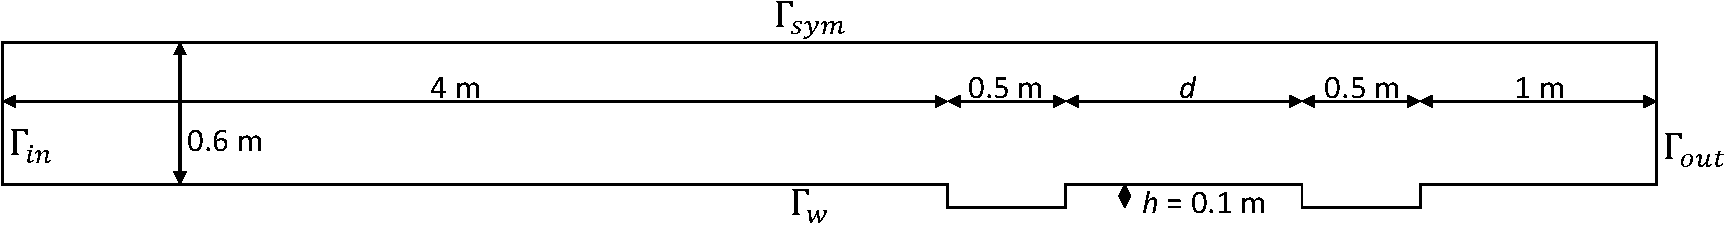
\includegraphics[width=\textwidth]{cavities_domain.pdf}
%	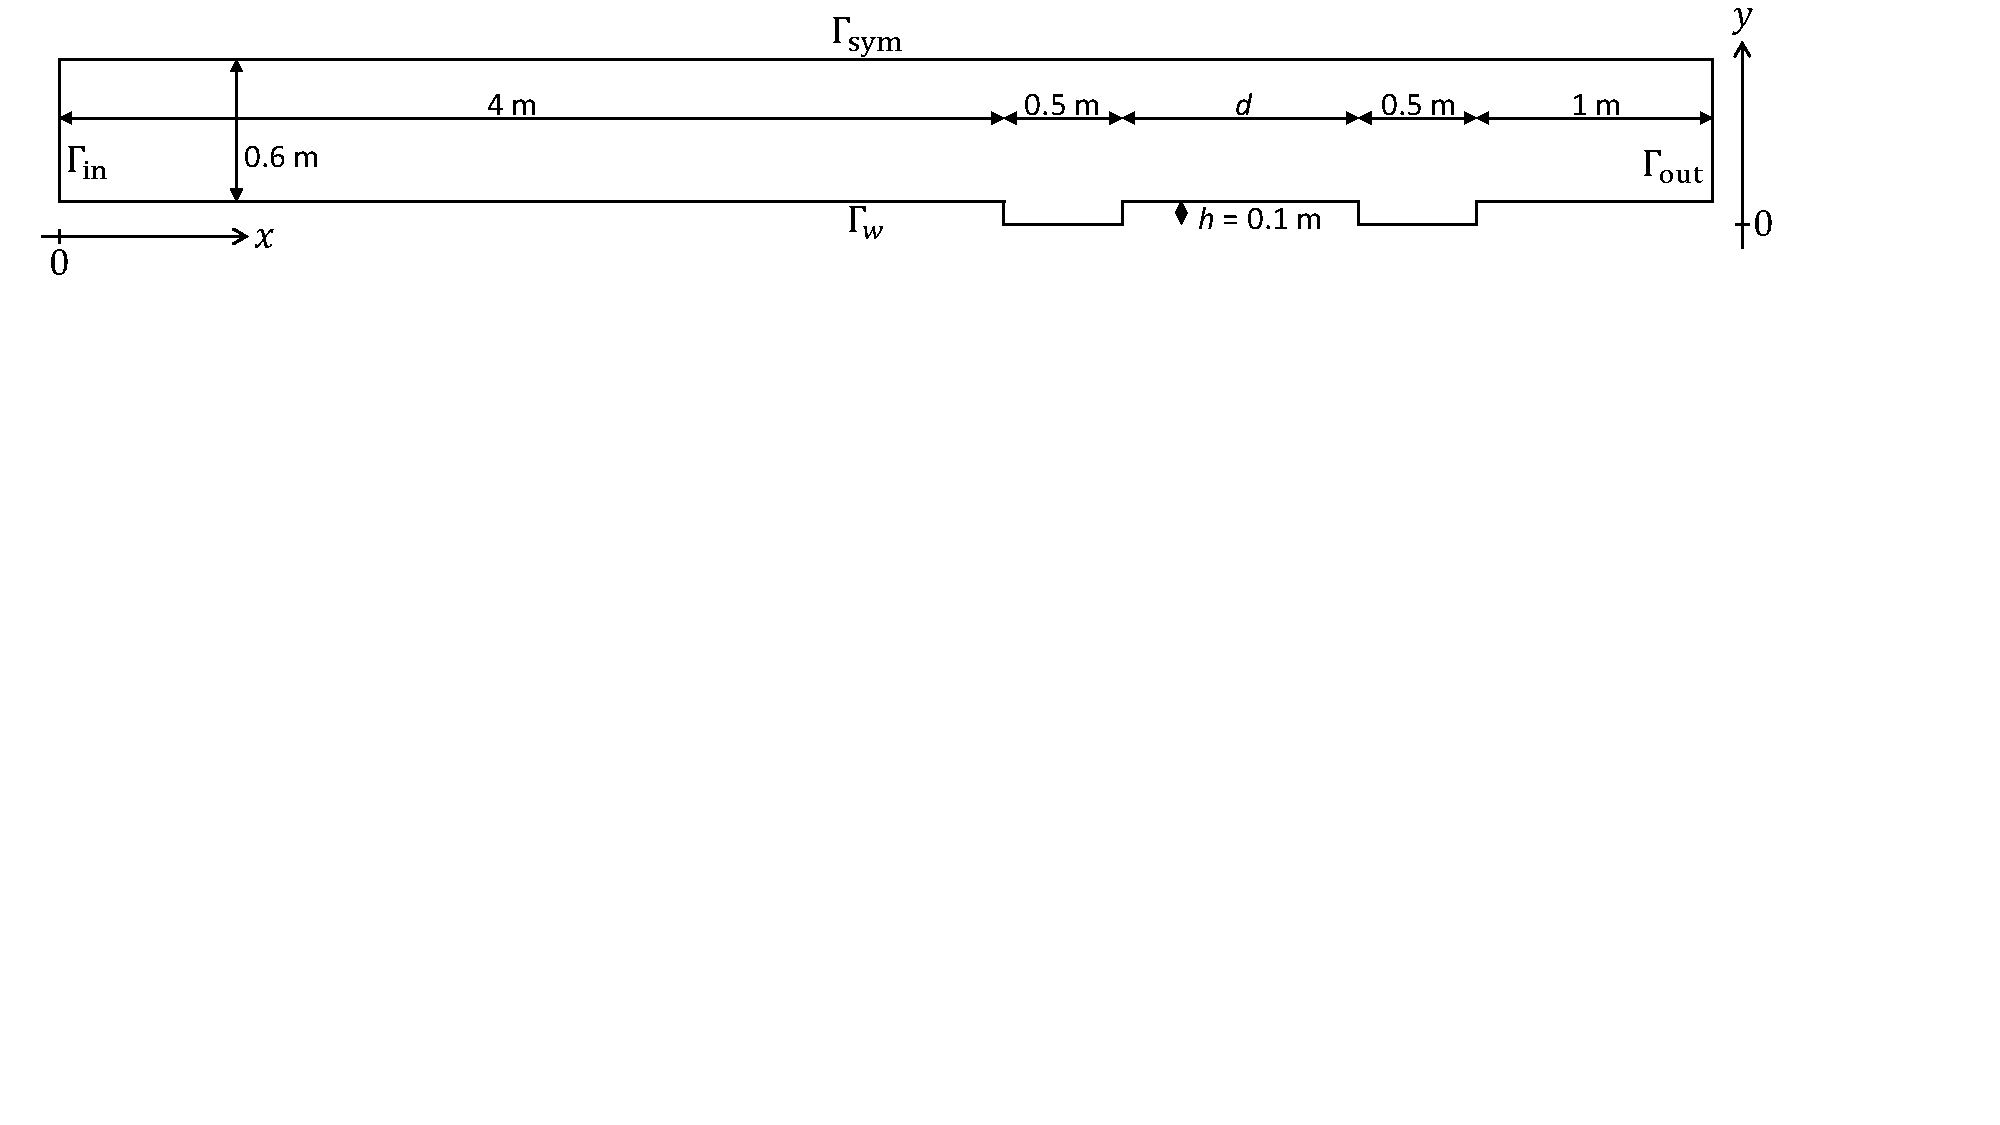
\includegraphics[width=\textwidth]{cavities_domain_axis.pdf}
	\caption[Free-flow domain $\Omega_\text{ff}$ in the cavities problem]{Free-flow domain $\Omega_\text{ff}$ in the cavities problem. The distance $d$ is varied from $\SI{0.05}{m}$ to $\SI{2}{m}$. For convenience we set the origin of the $x$-axis at the $\Gamma_\text{in}$ and the origin of the $y$-axis at the bottom of the cavities.}
	\label{fig:singledomain}
\end{figure}
The density of the fluid is $\varrho = \SI{1}{kg/m^3}$ and the kinematic viscosity is $\nu=\SI{e-5}{m^2/s}$, so that the Reynolds number is $Re=\num{6e5}$. We neglect the gravity contribution.

We want to see how the flow field in the second cavity is affected by the 
presence of the first cavity, depending on the distance $d$ between them, that 
has been varied from $\SI{0.05}{m}$ to $\SI{2}{m}$.

We simulate the time interval $[0, T_\text{end}]$, with $T_\text{end}=\SI{30}{s}$, such that the solution reaches an equilibrium, and an initial time-step $\Delta t = \SI{e-5}{s}$. We start from the initial 
conditions of uniform parallel flow for $y>h$ and no flow for $y\leq h$
\begin{equation}
	\mathbf{v} = [u_\text{init},0]^\mathrm{T}, \quad u_\text{init} =
	\begin{cases}
	u_\text{in} \quad&\text{if $y>h$}\\
	0 \quad&\text{if $y\leq h$}
	\end{cases}
\end{equation}
while we set in the whole $\Omega_\text{ff}$ $p=p_\text{ext}$, $k=k_\text{in}$ and $\omega=\omega_\text{in}$, estimated with the formulas~\eqref{eq:koic}.

Performing a sensitivity analysis, we choose a grid made of $\num{377x50}$ 
elements, with gradings in the inlet and outlet portions of the channel in order 
to have small uniform cells around the two cavities, with sizes of $\SI{5x3.3}{mm}$.
%Aggiungere qualcosa sulla sensitivity analysis

At a first glance the behaviour of the fluid in the two cavities is very 
similar, there is not any strong influence of the first one on the second one 
and the pattern of the velocity field is the same, as we see in Figure~\ref{fig:veld1}. 
%aggiungere cenno a quali recirculations ci sono e mettere le freccette 
%nell'immagine?
\begin{figure}
	\centering
	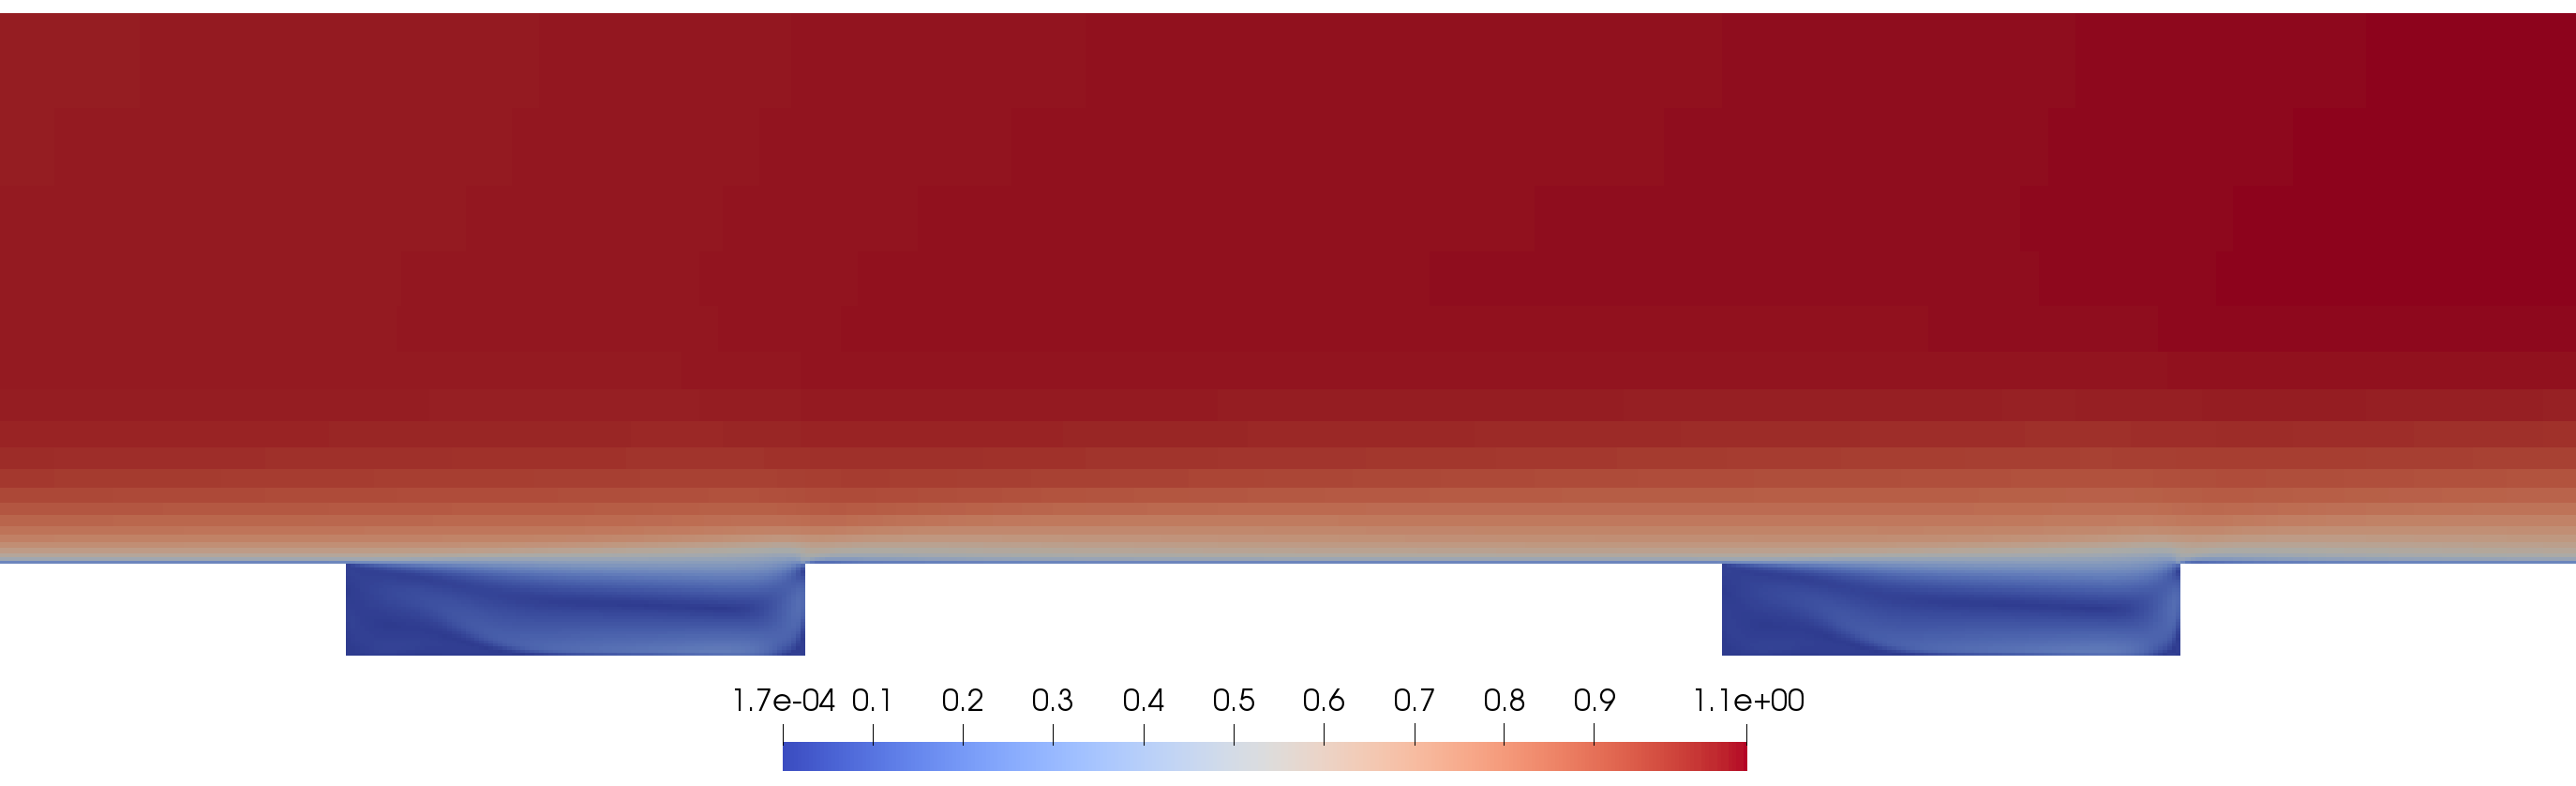
\includegraphics[width=\textwidth%, trim={0 0 0 6cm}, clip
	]{cavities_dist1_vel_report.png}
	\caption[Magnitude of the velocity field in the cavities problem]{Magnitude of the velocity field [$\si{m/s}$] around the cavities, with $d=\SI{1}{m}$ at $t=T_\text{end}$. $Re=\num{6e5}$.}
	\label{fig:veld1}
\end{figure}
In order to better analyse the results of the simulations, we compare the 
profiles of the velocity in the first cells above $y=h$. The velocity in these points drives the flow in the cavities, 
since we start from zero velocity inside them. Looking at the profiles in Figure~\ref{fig:velprofile1}, there is a positive 
peak of the velocity near the centre of each cavity, then, when the wall starts 
again, there is a negative peak, followed by a space, that we call recovery 
distance $d_{rec}$, of approximately $\SI{0.5}{m}$, in which there is a recovery 
of the value that the velocity had before the cavity. The values in the second 
cavity are slightly lower than the correspondent ones in the first cavity, but 
the shape is the same and this confirms the fact that the behaviour of the flow 
in the two cavities is the analogous.
\begin{figure}
	\centering
	% This file was created by matlab2tikz.
%
\definecolor{mycolor1}{rgb}{0.00000,0.44700,0.74100}%
%
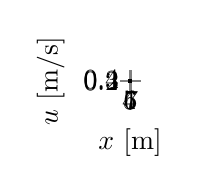
\begin{tikzpicture}

\begin{axis}[%
width=0.951\widthsette,
height=0.75\widthsette,
at={(0\widthsette,0\widthsette)},
scale only axis,
xmin=3.5,
xmax=7,
xlabel={$x$ [m]},
ymin=0.15,
ymax=0.4,
ylabel={$u$ [m/s]},
axis background/.style={fill=white},
xmajorgrids,
ymajorgrids
]
\addplot [color=black, line width=1.0pt, forget plot]
  table[row sep=crcr]{%
3.505	0.262676\\
3.51	0.262616\\
3.515	0.262616\\
3.52	0.262616\\
3.525	0.262616\\
3.53	0.262616\\
3.535	0.262616\\
3.54	0.262616\\
3.545	0.262616\\
3.55	0.262616\\
3.555	0.262616\\
3.56	0.262558\\
3.565	0.262558\\
3.57	0.262558\\
3.575	0.262558\\
3.58	0.262558\\
3.585	0.262558\\
3.59	0.262558\\
3.595	0.262558\\
3.6	0.262558\\
3.605	0.262503\\
3.61	0.262503\\
3.615	0.262503\\
3.62	0.262503\\
3.625	0.262503\\
3.63	0.262503\\
3.635	0.262503\\
3.64	0.262503\\
3.645	0.26245\\
3.65	0.26245\\
3.655	0.26245\\
3.66	0.26245\\
3.665	0.26245\\
3.67	0.26245\\
3.675	0.26245\\
3.68	0.26245\\
3.685	0.262399\\
3.69	0.262399\\
3.695	0.262399\\
3.7	0.262399\\
3.705	0.262399\\
3.71	0.262399\\
3.715	0.262399\\
3.72	0.262351\\
3.725	0.262351\\
3.73	0.262351\\
3.735	0.262351\\
3.74	0.262351\\
3.745	0.262351\\
3.75	0.262306\\
3.755	0.262306\\
3.76	0.262306\\
3.765	0.262306\\
3.77	0.262306\\
3.775	0.262265\\
3.78	0.262265\\
3.785	0.262265\\
3.79	0.262265\\
3.795	0.262265\\
3.8	0.262227\\
3.805	0.262227\\
3.81	0.262227\\
3.815	0.262227\\
3.82	0.262227\\
3.825	0.262195\\
3.83	0.262195\\
3.835	0.262195\\
3.84	0.262195\\
3.845	0.262168\\
3.85	0.262168\\
3.855	0.262168\\
3.86	0.262168\\
3.865	0.262148\\
3.87	0.262148\\
3.875	0.262148\\
3.88	0.262148\\
3.885	0.262137\\
3.89	0.262137\\
3.895	0.262137\\
3.9	0.262135\\
3.905	0.262135\\
3.91	0.262135\\
3.915	0.262145\\
3.92	0.262145\\
3.925	0.262168\\
3.93	0.262168\\
3.935	0.262168\\
3.94	0.262209\\
3.945	0.262209\\
3.95	0.262272\\
3.955	0.262272\\
3.96	0.262368\\
3.965	0.262368\\
3.97	0.262512\\
3.975	0.262728\\
3.98	0.262728\\
3.985	0.263067\\
3.99	0.263662\\
3.995	0.26509\\
4	0.268628\\
4.005	0.268628\\
4.01	0.27414\\
4.015	0.280032\\
4.02	0.285537\\
4.025	0.290514\\
4.03	0.294956\\
4.035	0.298941\\
4.04	0.302551\\
4.045	0.305844\\
4.05	0.308863\\
4.055	0.311641\\
4.06	0.314202\\
4.065	0.316568\\
4.07	0.318763\\
4.075	0.320816\\
4.08	0.322754\\
4.085	0.324599\\
4.09	0.326371\\
4.095	0.328094\\
4.1	0.329791\\
4.105	0.331472\\
4.11	0.333147\\
4.115	0.334828\\
4.12	0.33652\\
4.125	0.33823\\
4.13	0.339963\\
4.135	0.341723\\
4.14	0.343509\\
4.145	0.345319\\
4.15	0.347147\\
4.155	0.348985\\
4.16	0.350827\\
4.165	0.352663\\
4.17	0.354484\\
4.175	0.356285\\
4.18	0.358057\\
4.185	0.359792\\
4.19	0.361487\\
4.195	0.363137\\
4.2	0.364737\\
4.205	0.366281\\
4.21	0.367768\\
4.215	0.369193\\
4.22	0.370556\\
4.225	0.371852\\
4.23	0.373082\\
4.235	0.374244\\
4.24	0.375337\\
4.245	0.376361\\
4.25	0.377316\\
4.255	0.378202\\
4.26	0.37902\\
4.265	0.379771\\
4.27	0.380456\\
4.275	0.381076\\
4.28	0.381633\\
4.285	0.38213\\
4.29	0.382567\\
4.295	0.382947\\
4.3	0.383274\\
4.305	0.383549\\
4.31	0.383777\\
4.315	0.38396\\
4.32	0.384103\\
4.325	0.384211\\
4.33	0.384287\\
4.335	0.384334\\
4.34	0.384355\\
4.345	0.384354\\
4.35	0.384333\\
4.355	0.384293\\
4.36	0.384235\\
4.365	0.38416\\
4.37	0.384064\\
4.375	0.383945\\
4.38	0.383796\\
4.385	0.383606\\
4.39	0.383366\\
4.395	0.383059\\
4.4	0.382666\\
4.405	0.382164\\
4.41	0.381524\\
4.415	0.380707\\
4.42	0.379663\\
4.425	0.378339\\
4.43	0.376682\\
4.435	0.374643\\
4.44	0.372186\\
4.445	0.369265\\
4.45	0.365813\\
4.455	0.361743\\
4.46	0.356928\\
4.465	0.351207\\
4.47	0.344355\\
4.475	0.336065\\
4.48	0.325962\\
4.485	0.313661\\
4.49	0.298724\\
4.495	0.282999\\
4.5	0.295616\\
4.505	0.264581\\
4.51	0.193707\\
4.515	0.16835\\
4.52	0.163515\\
4.525	0.167251\\
4.53	0.173801\\
4.535	0.181008\\
4.54	0.188012\\
4.545	0.194581\\
4.55	0.194581\\
4.555	0.200482\\
4.56	0.205777\\
4.565	0.210593\\
4.57	0.210593\\
4.575	0.214974\\
4.58	0.218972\\
4.585	0.222644\\
4.59	0.222644\\
4.595	0.226024\\
4.6	0.229138\\
4.605	0.229138\\
4.61	0.232011\\
4.615	0.234665\\
4.62	0.234665\\
4.625	0.237118\\
4.63	0.237118\\
4.635	0.239386\\
4.64	0.241484\\
4.645	0.241484\\
4.65	0.243426\\
4.655	0.243426\\
4.66	0.245225\\
4.665	0.245225\\
4.67	0.24689\\
4.675	0.24689\\
4.68	0.248431\\
4.685	0.249852\\
4.69	0.249852\\
4.695	0.251162\\
4.7	0.251162\\
4.705	0.252364\\
4.71	0.252364\\
4.715	0.253465\\
4.72	0.253465\\
4.725	0.253465\\
4.73	0.25447\\
4.735	0.25447\\
4.74	0.255385\\
4.745	0.255385\\
4.75	0.256216\\
4.755	0.256216\\
4.76	0.256971\\
4.765	0.256971\\
4.77	0.257656\\
4.775	0.257656\\
4.78	0.257656\\
4.785	0.258274\\
4.79	0.258274\\
4.795	0.258831\\
4.8	0.258831\\
4.805	0.258831\\
4.81	0.25933\\
4.815	0.25933\\
4.82	0.259773\\
4.825	0.259773\\
4.83	0.259773\\
4.835	0.260165\\
4.84	0.260165\\
4.845	0.260165\\
4.85	0.260507\\
4.855	0.260507\\
4.86	0.260804\\
4.865	0.260804\\
4.87	0.260804\\
4.875	0.261058\\
4.88	0.261058\\
4.885	0.261058\\
4.89	0.261272\\
4.895	0.261272\\
4.9	0.261272\\
4.905	0.26145\\
4.91	0.26145\\
4.915	0.26145\\
4.92	0.261597\\
4.925	0.261597\\
4.93	0.261597\\
4.935	0.261716\\
4.94	0.261716\\
4.945	0.261716\\
4.95	0.26181\\
4.955	0.26181\\
4.96	0.26181\\
4.965	0.26181\\
4.97	0.261883\\
4.975	0.261883\\
4.98	0.261883\\
4.985	0.26194\\
4.99	0.26194\\
4.995	0.26194\\
5	0.26194\\
5.005	0.261979\\
5.01	0.261979\\
5.015	0.261979\\
5.02	0.261996\\
5.025	0.261996\\
5.03	0.261996\\
5.035	0.261995\\
5.04	0.261995\\
5.045	0.261995\\
5.05	0.261995\\
5.055	0.261983\\
5.06	0.261983\\
5.065	0.261983\\
5.07	0.261961\\
5.075	0.261961\\
5.08	0.261961\\
5.085	0.26193\\
5.09	0.26193\\
5.095	0.26193\\
5.1	0.261892\\
5.105	0.261892\\
5.11	0.261892\\
5.115	0.26185\\
5.12	0.26185\\
5.125	0.26185\\
5.13	0.261804\\
5.135	0.261804\\
5.14	0.261804\\
5.145	0.261757\\
5.15	0.261757\\
5.155	0.261709\\
5.16	0.261709\\
5.165	0.261709\\
5.17	0.261661\\
5.175	0.261661\\
5.18	0.261661\\
5.185	0.261614\\
5.19	0.261614\\
5.195	0.261568\\
5.2	0.261568\\
5.205	0.261568\\
5.21	0.261522\\
5.215	0.261522\\
5.22	0.261476\\
5.225	0.261476\\
5.23	0.261476\\
5.235	0.261432\\
5.24	0.261432\\
5.245	0.261388\\
5.25	0.261388\\
5.255	0.261344\\
5.26	0.261344\\
5.265	0.261302\\
5.27	0.261302\\
5.275	0.26126\\
5.28	0.26126\\
5.285	0.26126\\
5.29	0.261219\\
5.295	0.261219\\
5.3	0.261179\\
5.305	0.261179\\
5.31	0.261141\\
5.315	0.261141\\
5.32	0.261103\\
5.325	0.261067\\
5.33	0.261067\\
5.335	0.261032\\
5.34	0.261032\\
5.345	0.260999\\
5.35	0.260999\\
5.355	0.260967\\
5.36	0.260967\\
5.365	0.260937\\
5.37	0.26091\\
5.375	0.26091\\
5.38	0.260884\\
5.385	0.260884\\
5.39	0.260861\\
5.395	0.260841\\
5.4	0.260841\\
5.405	0.260825\\
5.41	0.260813\\
5.415	0.260813\\
5.42	0.260805\\
5.425	0.260803\\
5.43	0.260807\\
5.435	0.260807\\
5.44	0.260818\\
5.445	0.260838\\
5.45	0.260869\\
5.455	0.260869\\
5.46	0.260914\\
5.465	0.260979\\
5.47	0.261071\\
5.475	0.261202\\
5.48	0.261396\\
5.485	0.261698\\
5.49	0.262222\\
5.495	0.26347\\
5.5	0.266629\\
5.505	0.266629\\
5.51	0.271595\\
5.515	0.276913\\
5.52	0.281899\\
5.525	0.28642\\
5.53	0.290467\\
5.535	0.294107\\
5.54	0.297413\\
5.545	0.300435\\
5.55	0.303213\\
5.555	0.305775\\
5.56	0.30814\\
5.565	0.310327\\
5.57	0.312362\\
5.575	0.314269\\
5.58	0.316073\\
5.585	0.317791\\
5.59	0.319442\\
5.595	0.321042\\
5.6	0.322609\\
5.605	0.324163\\
5.61	0.325711\\
5.615	0.327261\\
5.62	0.328822\\
5.625	0.330398\\
5.63	0.331996\\
5.635	0.333617\\
5.64	0.335264\\
5.645	0.336936\\
5.65	0.338634\\
5.655	0.340354\\
5.66	0.342088\\
5.665	0.34383\\
5.67	0.345572\\
5.675	0.347305\\
5.68	0.349021\\
5.685	0.350713\\
5.69	0.352373\\
5.695	0.353994\\
5.7	0.355573\\
5.705	0.357103\\
5.71	0.358579\\
5.715	0.36\\
5.72	0.361363\\
5.725	0.362667\\
5.73	0.363909\\
5.735	0.365089\\
5.74	0.366205\\
5.745	0.367258\\
5.75	0.368245\\
5.755	0.369167\\
5.76	0.370024\\
5.765	0.370815\\
5.77	0.371541\\
5.775	0.372204\\
5.78	0.372803\\
5.785	0.373342\\
5.79	0.37382\\
5.795	0.374241\\
5.8	0.374607\\
5.805	0.374921\\
5.81	0.375186\\
5.815	0.375404\\
5.82	0.375579\\
5.825	0.375716\\
5.83	0.375816\\
5.835	0.375883\\
5.84	0.375918\\
5.845	0.375925\\
5.85	0.375907\\
5.855	0.375866\\
5.86	0.3758\\
5.865	0.375709\\
5.87	0.37559\\
5.875	0.375439\\
5.88	0.375247\\
5.885	0.375009\\
5.89	0.374712\\
5.895	0.374345\\
5.9	0.373886\\
5.905	0.37331\\
5.91	0.372592\\
5.915	0.371699\\
5.92	0.370589\\
5.925	0.369218\\
5.93	0.367541\\
5.935	0.365513\\
5.94	0.363089\\
5.945	0.36021\\
5.95	0.356812\\
5.955	0.352805\\
5.96	0.348069\\
5.965	0.342443\\
5.97	0.335705\\
5.975	0.327557\\
5.98	0.317633\\
5.985	0.305563\\
5.99	0.290921\\
5.995	0.275548\\
6	0.288264\\
6.005	0.189663\\
6.01	0.189663\\
6.015	0.164357\\
6.02	0.160921\\
6.025	0.167072\\
6.03	0.167072\\
6.035	0.176188\\
6.04	0.185964\\
6.045	0.185964\\
6.05	0.195421\\
6.055	0.195421\\
6.06	0.203955\\
6.065	0.203955\\
6.07	0.211669\\
6.075	0.211669\\
6.08	0.21859\\
6.085	0.21859\\
6.09	0.21859\\
6.095	0.224818\\
6.1	0.224818\\
6.105	0.224818\\
6.11	0.230405\\
6.115	0.230405\\
6.12	0.230405\\
6.125	0.23541\\
6.13	0.23541\\
6.135	0.23541\\
6.14	0.239845\\
6.145	0.239845\\
6.15	0.239845\\
6.155	0.239845\\
6.16	0.24374\\
6.165	0.24374\\
6.17	0.24374\\
6.175	0.24374\\
6.18	0.24713\\
6.185	0.24713\\
6.19	0.24713\\
6.195	0.24713\\
6.2	0.24713\\
6.205	0.250021\\
6.21	0.250021\\
6.215	0.250021\\
6.22	0.250021\\
6.225	0.250021\\
6.23	0.252439\\
6.235	0.252439\\
6.24	0.252439\\
6.245	0.252439\\
6.25	0.252439\\
6.255	0.254431\\
6.26	0.254431\\
6.265	0.254431\\
6.27	0.254431\\
6.275	0.254431\\
6.28	0.254431\\
6.285	0.256028\\
6.29	0.256028\\
6.295	0.256028\\
6.3	0.256028\\
6.305	0.256028\\
6.31	0.256028\\
6.315	0.256028\\
6.32	0.257261\\
6.325	0.257261\\
6.33	0.257261\\
6.335	0.257261\\
6.34	0.257261\\
6.345	0.257261\\
6.35	0.257261\\
6.355	0.257261\\
6.36	0.258168\\
6.365	0.258168\\
6.37	0.258168\\
6.375	0.258168\\
6.38	0.258168\\
6.385	0.258168\\
6.39	0.258168\\
6.395	0.258168\\
6.4	0.258804\\
6.405	0.258804\\
6.41	0.258804\\
6.415	0.258804\\
6.42	0.258804\\
6.425	0.258804\\
6.43	0.258804\\
6.435	0.258804\\
6.44	0.258804\\
6.445	0.259215\\
6.45	0.259215\\
6.455	0.259215\\
6.46	0.259215\\
6.465	0.259215\\
6.47	0.259215\\
6.475	0.259215\\
6.48	0.259215\\
6.485	0.259215\\
6.49	0.259449\\
6.495	0.259449\\
6.5	0.259449\\
6.505	0.259449\\
6.51	0.259449\\
6.515	0.259449\\
6.52	0.259449\\
6.525	0.259449\\
6.53	0.259449\\
6.535	0.259449\\
6.54	0.259449\\
6.545	0.25952\\
6.55	0.25952\\
6.555	0.25952\\
6.56	0.25952\\
6.565	0.25952\\
6.57	0.25952\\
6.575	0.25952\\
6.58	0.25952\\
6.585	0.25952\\
6.59	0.25952\\
6.595	0.25952\\
6.6	0.25952\\
6.605	0.259476\\
6.61	0.259476\\
6.615	0.259476\\
6.62	0.259476\\
6.625	0.259476\\
6.63	0.259476\\
6.635	0.259476\\
6.64	0.259476\\
6.645	0.259476\\
6.65	0.259476\\
6.655	0.259476\\
6.66	0.259476\\
6.665	0.259476\\
6.67	0.259376\\
6.675	0.259376\\
6.68	0.259376\\
6.685	0.259376\\
6.69	0.259376\\
6.695	0.259376\\
6.7	0.259376\\
6.705	0.259376\\
6.71	0.259376\\
6.715	0.259376\\
6.72	0.259376\\
6.725	0.259376\\
6.73	0.259376\\
6.735	0.259376\\
6.74	0.259219\\
6.745	0.259219\\
6.75	0.259219\\
6.755	0.259219\\
6.76	0.259219\\
6.765	0.259219\\
6.77	0.259219\\
6.775	0.259219\\
6.78	0.259219\\
6.785	0.259219\\
6.79	0.259219\\
6.795	0.259219\\
6.8	0.259219\\
6.805	0.259219\\
6.81	0.259219\\
6.815	0.259219\\
6.82	0.25916\\
6.825	0.25916\\
6.83	0.25916\\
6.835	0.25916\\
6.84	0.25916\\
6.845	0.25916\\
6.85	0.25916\\
6.855	0.25916\\
6.86	0.25916\\
6.865	0.25916\\
6.87	0.25916\\
6.875	0.25916\\
6.88	0.25916\\
6.885	0.25916\\
6.89	0.25916\\
6.895	0.25916\\
6.9	0.25916\\
6.905	0.259157\\
6.91	0.259157\\
6.915	0.259157\\
6.92	0.259157\\
6.925	0.259157\\
6.93	0.259157\\
6.935	0.259157\\
6.94	0.259157\\
6.945	0.259157\\
6.95	0.259157\\
6.955	0.259157\\
6.96	0.259157\\
6.965	0.259157\\
6.97	0.259157\\
6.975	0.259157\\
6.98	0.259157\\
6.985	0.259157\\
6.99	0.259157\\
6.995	0.259157\\
7	0.259157\\
};
\end{axis}
\end{tikzpicture}%
	\caption[Profile of the $u$ component of the velocity at $y=h$ in the cavities problem]{Profile of the $u$ component of the velocity at $y=h$, with a distance $d=\SI{1}{m}$ between cavities, at $t=T_\text{end}$. $Re = \num{6e5}$.}
	\label{fig:velprofile1}
\end{figure}

The peaks above the cavities are due to the fact that those sections of the profile are not 
touching the wall, so the wall friction is not highly affecting the velocity as it is
in the other sections and this allows the velocity to reach higher values.
When a cavity is over and the wall begins there is a sudden decrease in the 
velocity because before the corner of the cavity the flow is split into a 
portion that goes down and generates the recirculation and another portion that 
instead goes up, as we observe in Figure~\ref{fig:vel_split}.
\begin{figure}
	\centering
	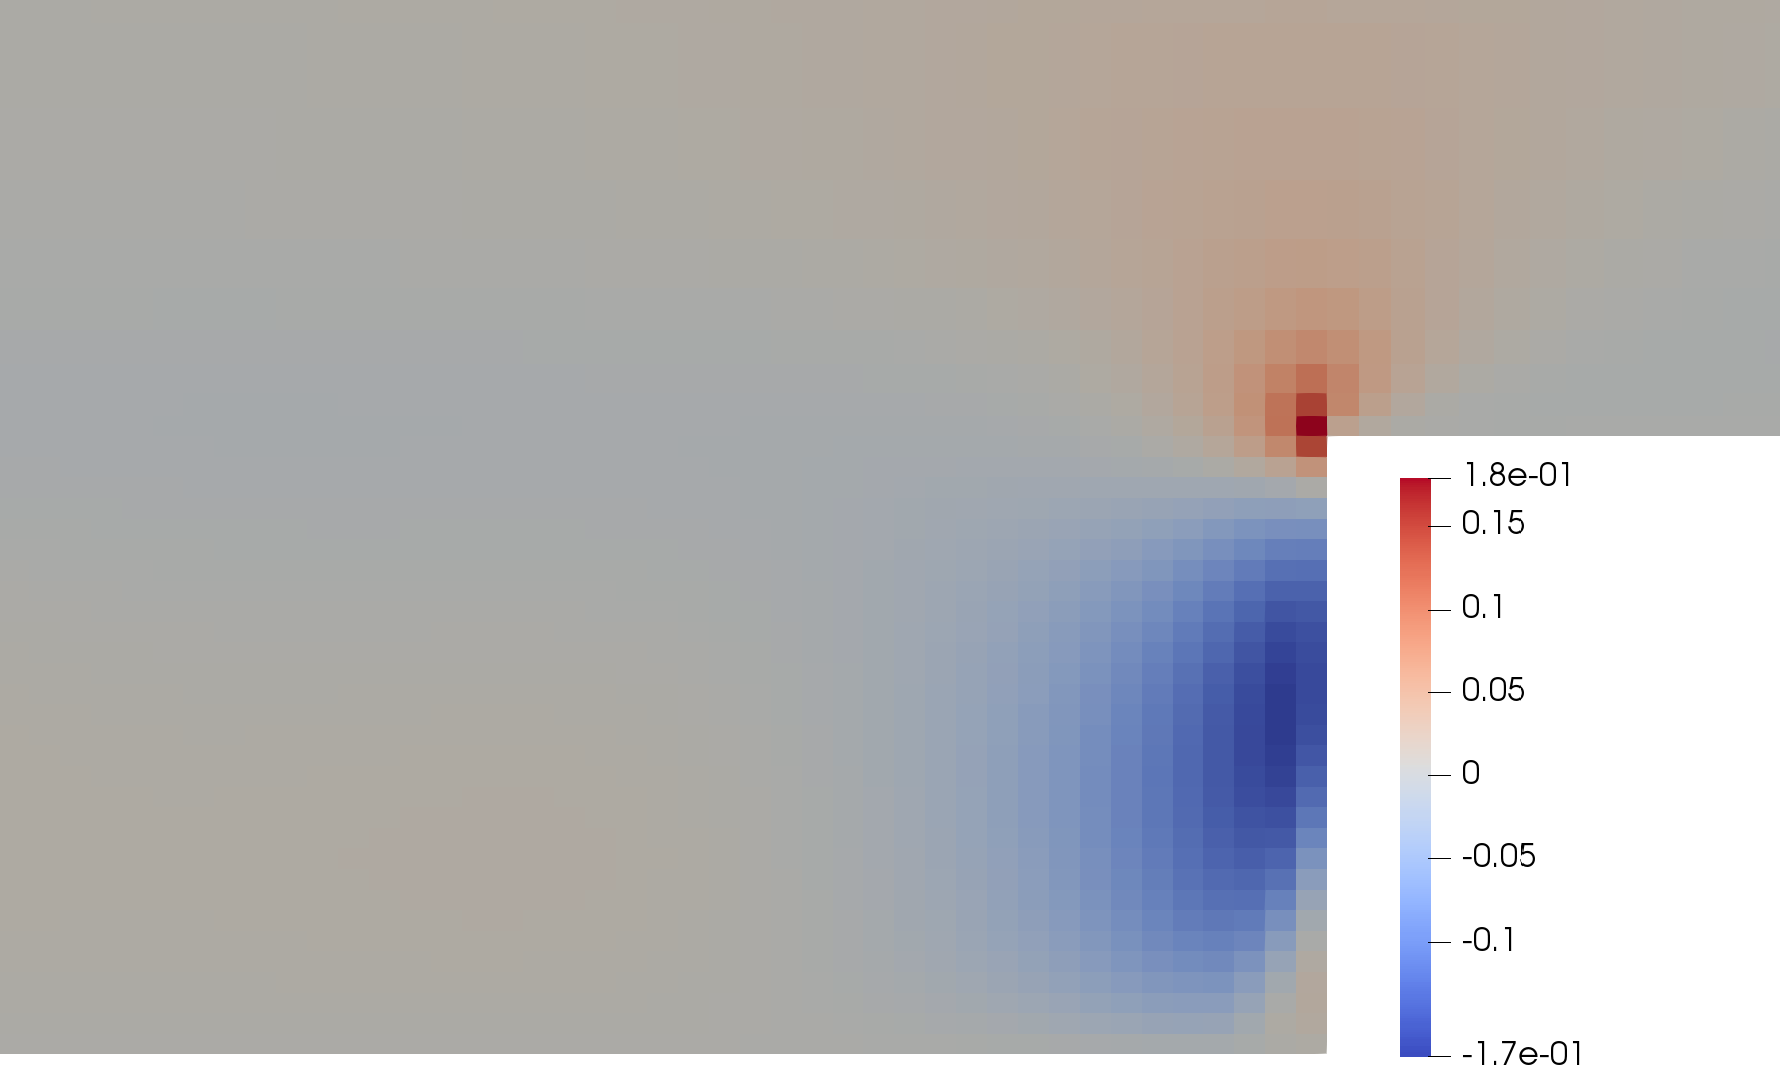
\includegraphics[width=0.7\textwidth]{cavities_vel_split_report.png}
	\caption[$v$-component of the velocity near end of a cavity in the cavities problem]{$v$-component of the velocity $\si{m/s}$ near end of a cavity. It can be observed that the flow splits. $Re = \num{6e5}$.}
	\label{fig:vel_split}
\end{figure}
This change in the flow direction implies a reduction of the $u$ component of the velocity. After the 
distance $d_{rec}$ the effect of the wall has restored the boundary layer that 
there was before the cavity. If $d < d_{rec}$, i.e. the distance between the 
cavities is smaller than the recovery distance, the flow in the second 
cavity will be slower because it will be driven by lower velocities.

We report in Figure~\ref{fig:velpeaks} the maximum values of the $u$-component 
of the velocity in correspondence of the peak above the second cavity, depending 
of the distance between the cavities.
\begin{figure}
	\centering
	% This file was created by matlab2tikz.
%
\definecolor{mycolor1}{rgb}{0.00000,0.44700,0.74100}%
%
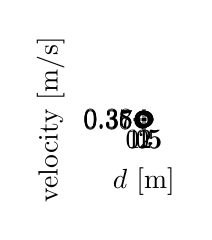
\begin{tikzpicture}

\begin{axis}[%
width=0.951\widthsette,
height=0.75\widthsette,
at={(0\widthsette,0\widthsette)},
scale only axis,
xmin=0,
xmax=2,
xlabel={$d$ [m]},
ymin=0.35,
ymax=0.38,
ylabel={velocity [m/s]},
axis background/.style={fill=white},
xmajorgrids,
ymajorgrids,
yticklabel style={/pgf/number format/.cd,fixed,precision=3}
]
\addplot [color=black, line width=1.0pt, mark size=2.5pt, mark=o, mark options={solid, black}, forget plot]
  table[row sep=crcr]{%
0.05	0.352715\\
0.2	0.371891\\
0.3	0.375066\\
0.5	0.376806\\
1	0.375925\\
1.5	0.374456\\
2	0.373188\\
};
\end{axis}
\end{tikzpicture}%
	\caption[Relation between the maximum velocity above the second cavity and 
	the distance between the cavities]{Relation between the maximum velocity in the peak above the second cavity and the distance $d$ between the cavities.}
	\label{fig:velpeaks}
\end{figure}
We see that if $d < d_{rec}$ the velocity is affected by the presence of 
the first cavity and so its value is lower. For $d>d_{rec}$ the velocity is 
slightly decreasing as $d$ increases; this fact is due to the turbulence that 
is generated near the end of the first cavity. As it can be seen in 
Figure~\ref{fig:kd1}, the turbulent kinetic energy that is generated from the 
first cavity is transported towards the second one, leading to an increased 
thickness of the boundary layer as we move in the $x$-direction.
\begin{figure}
	\centering
	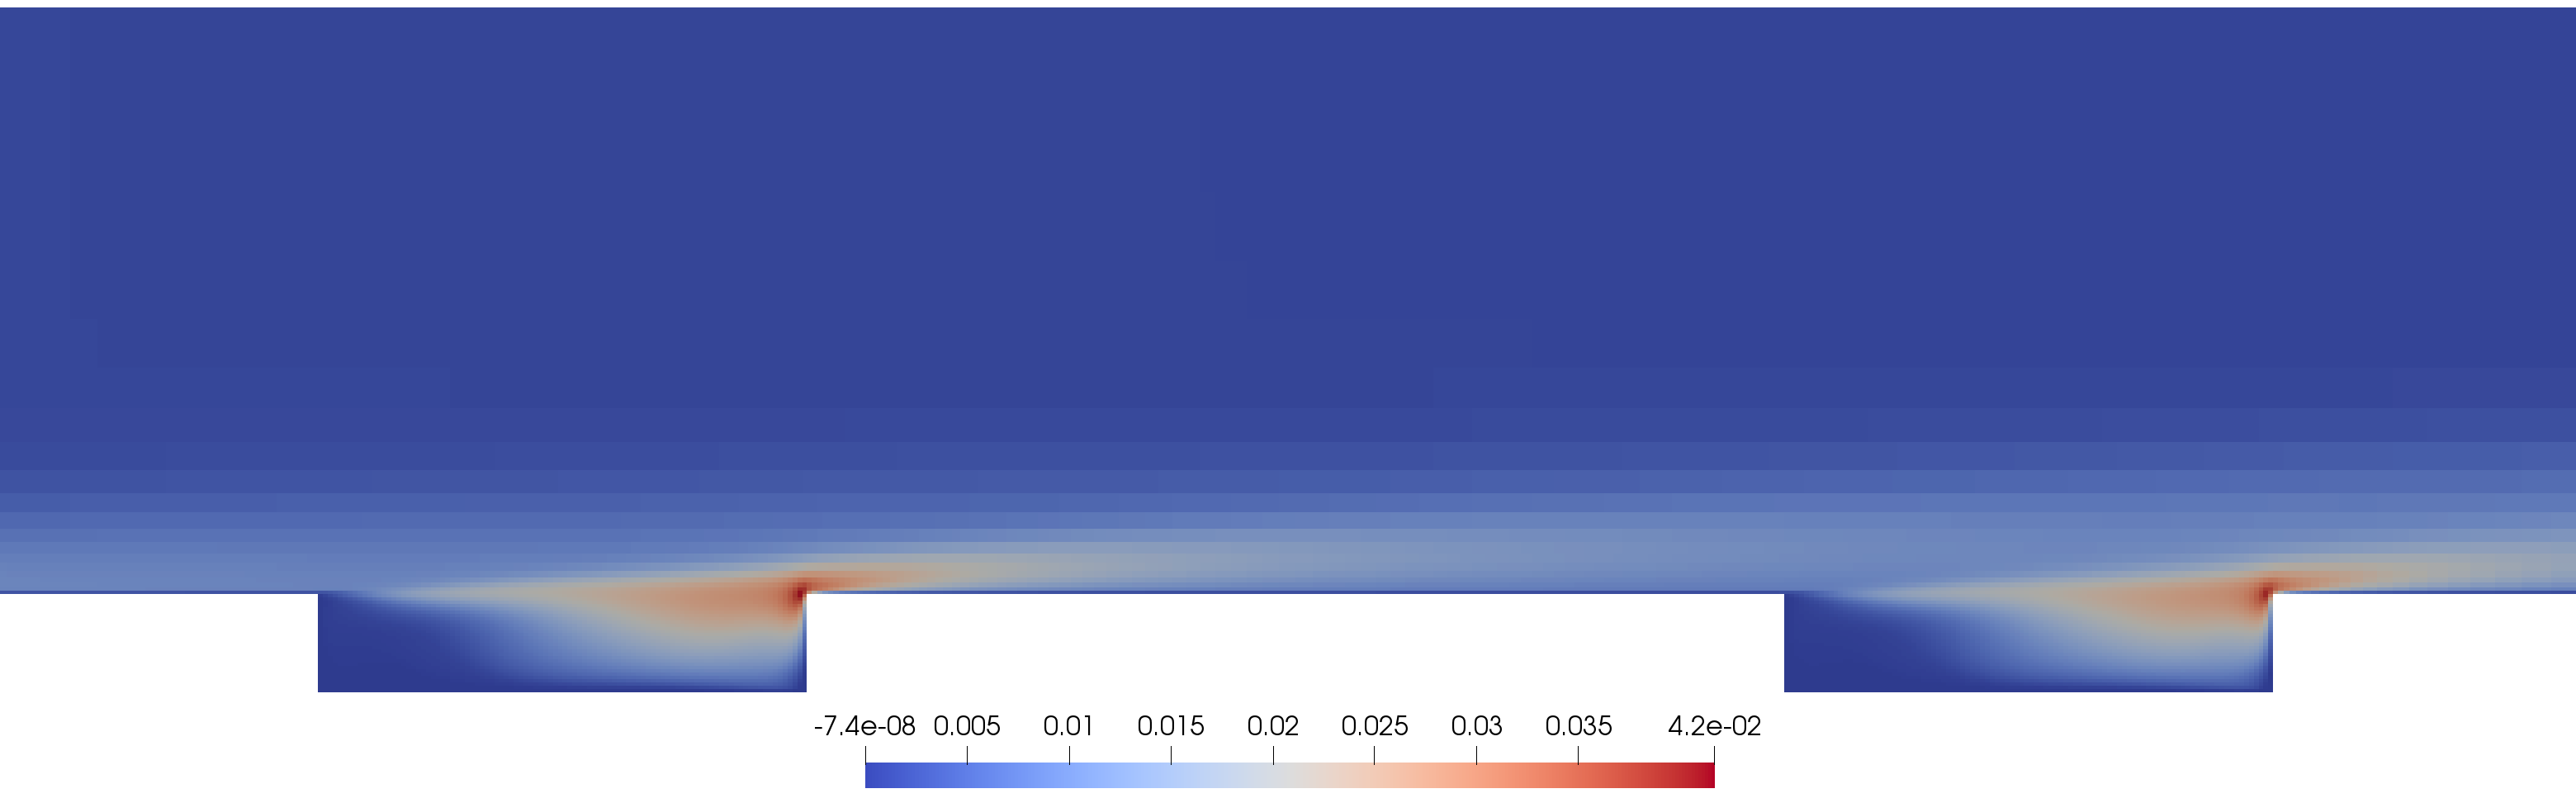
\includegraphics[width=\textwidth,% trim={0 0 0 7cm}, clip 
	]{cavities_dist1_k_report.png}
	\caption[Turbulen kinetic energy in the cavities problem]{Turbulent kinetic energy [$\si{m^2/s^2}$] around the cavities with $d=\SI{1}{m}$, at $t=T_\text{end}$. $Re=\num{6e5}$.}
	\label{fig:kd1}
\end{figure}
%
\subsection{Coupled problem}
%A more complex result.